% =====================================================================
%  PARTE DE VALENTINA  --  se incluye desde main.tex con % =====================================================================
%  PARTE DE VALENTINA  --  se incluye desde main.tex con % =====================================================================
%  PARTE DE VALENTINA  --  se incluye desde main.tex con % =====================================================================
%  PARTE DE VALENTINA  --  se incluye desde main.tex con \input{Valentina/valentina}
%  Contenido: Metodología, Análisis Gráfico (Colab/Conda) y Conclusiones
%
%  Reglas para editar sin romper la compilación:
%   * NO escribir \documentclass, \begin{document} ni \end{document} aquí.
%   * Las figuras están en ../imagenes/ y se llaman sólo por su nombre
%     (main.tex ya define \graphicspath{{imagenes/}}).
%   * Referenciar figuras con Figura~\ref{fig:...}, nunca "la figura de abajo".
% =====================================================================

\section{Metodología}
\fontsize{12}{14}\selectfont
% TODO (Valentina): pegar aquí la redacción de la metodología.

\subsection{Recolección de datos}
\textit{[Redacción pendiente: búsqueda en CAS-SciFinder, compuestos e indicadores asignados, consolidación en Excel con formato Tabla.]}

\subsection{Limpieza y procesamiento en Python}
\textit{[Redacción pendiente: Google Colab con Pandas, NumPy, Matplotlib, Seaborn y Plotly; filtrado de los compuestos de interés, conversión de comas decimales, tratamiento de valores nulos y atípicos.]}

\subsection{Análisis estadístico}
\textit{[Redacción pendiente: correlación de Spearman (no paramétrica, robusta a valores atípicos y relaciones monótonas no lineales), regresiones lineales con intervalo de confianza del 95\,\% y distribuciones por tipo de reacción y medio.]}

\section{Resultados y Discusión}
\fontsize{12}{14}\selectfont

\subsection{Correlación entre propiedades}
% TODO (Valentina): interpretar los coeficientes más fuertes (positivos y negativos).
La Figura~\ref{fig:heatmap} presenta la matriz de correlación de Spearman entre
las propiedades fisicoquímicas, y la Figura~\ref{fig:clustermap} agrupa
jerárquicamente las variables con comportamiento similar.
\textit{[Interpretación pendiente.]}

\begin{figure}[htbp]
	\centering
	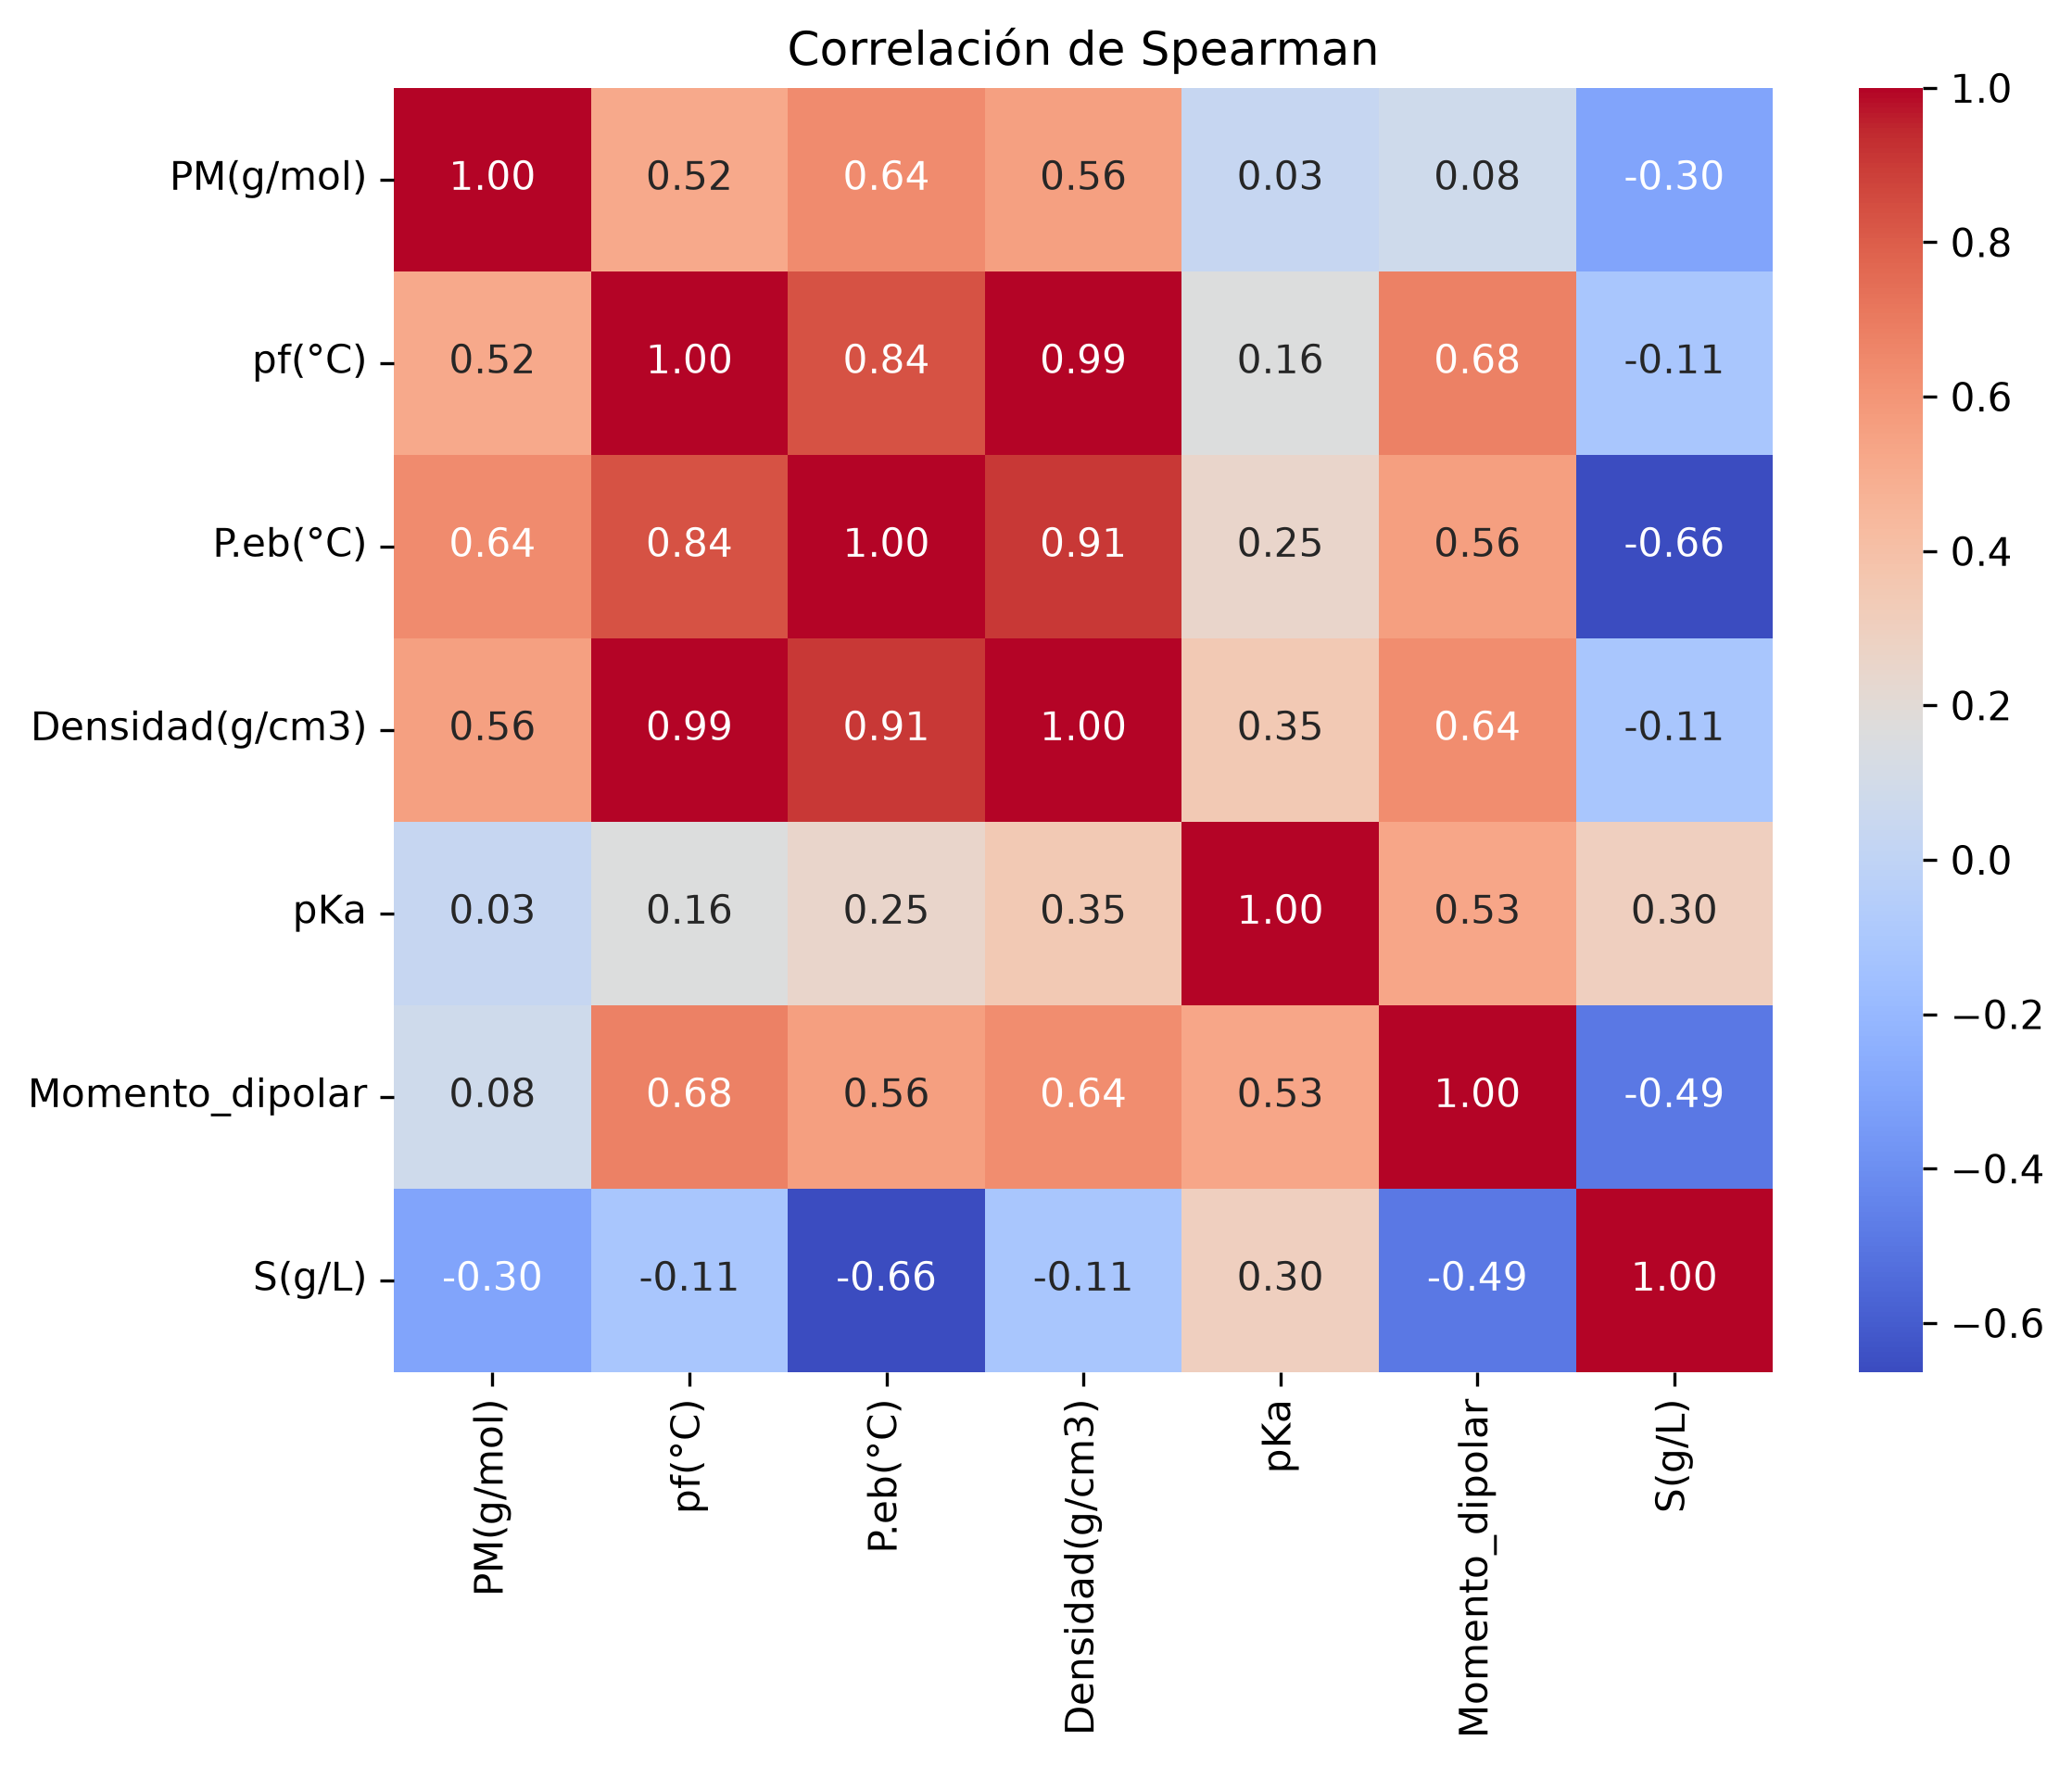
\includegraphics[width=\columnwidth]{01_heatmap_spearman.png}
	\caption{Matriz de correlación de Spearman entre las propiedades fisicoquímicas.}
	\label{fig:heatmap}
\end{figure}

\begin{figure}[htbp]
	\centering
	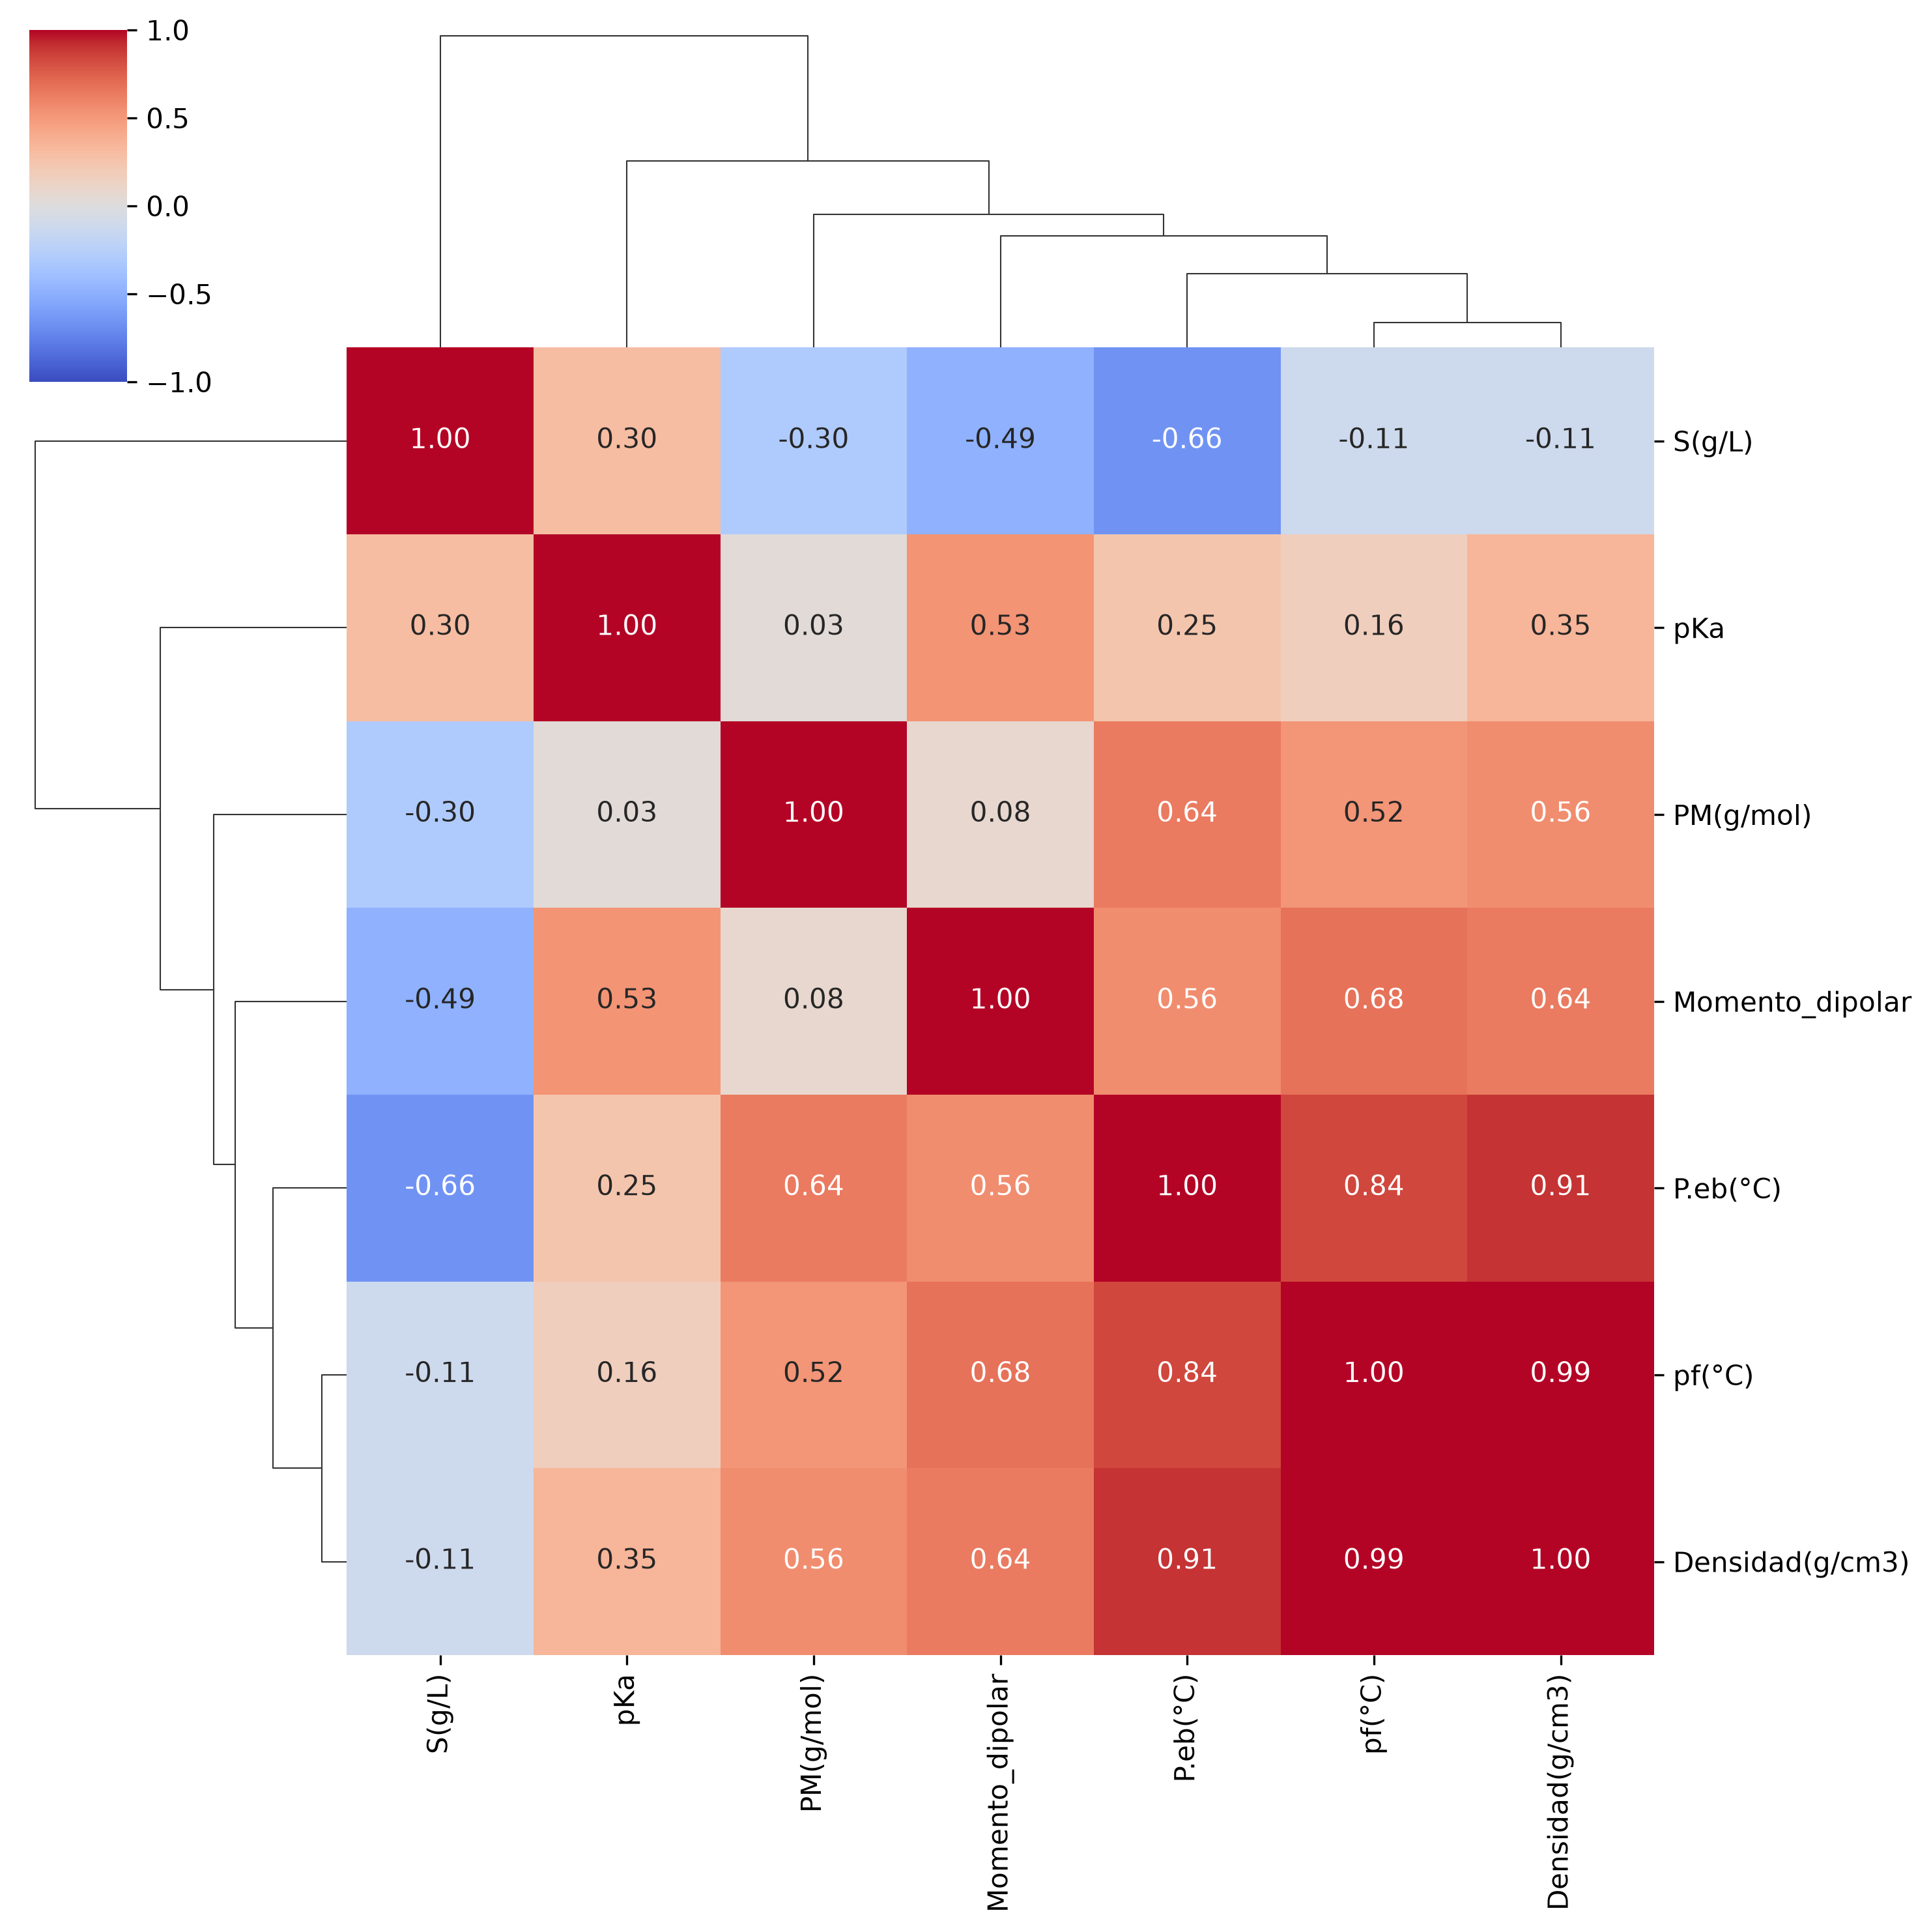
\includegraphics[width=\columnwidth]{02_clustermap_spearman.png}
	\caption{Mapa de agrupamiento jerárquico de la correlación de Spearman.}
	\label{fig:clustermap}
\end{figure}

\subsection{Tendencias entre propiedades}
% TODO (Valentina): discutir cada regresión en términos de fuerzas intermoleculares.
Las Figuras~\ref{fig:pf-dens}--\ref{fig:dip-peb} muestran las regresiones
lineales entre pares de propiedades, con su intervalo de confianza.
\textit{[Interpretación pendiente.]}

\begin{figure}[htbp]
	\centering
	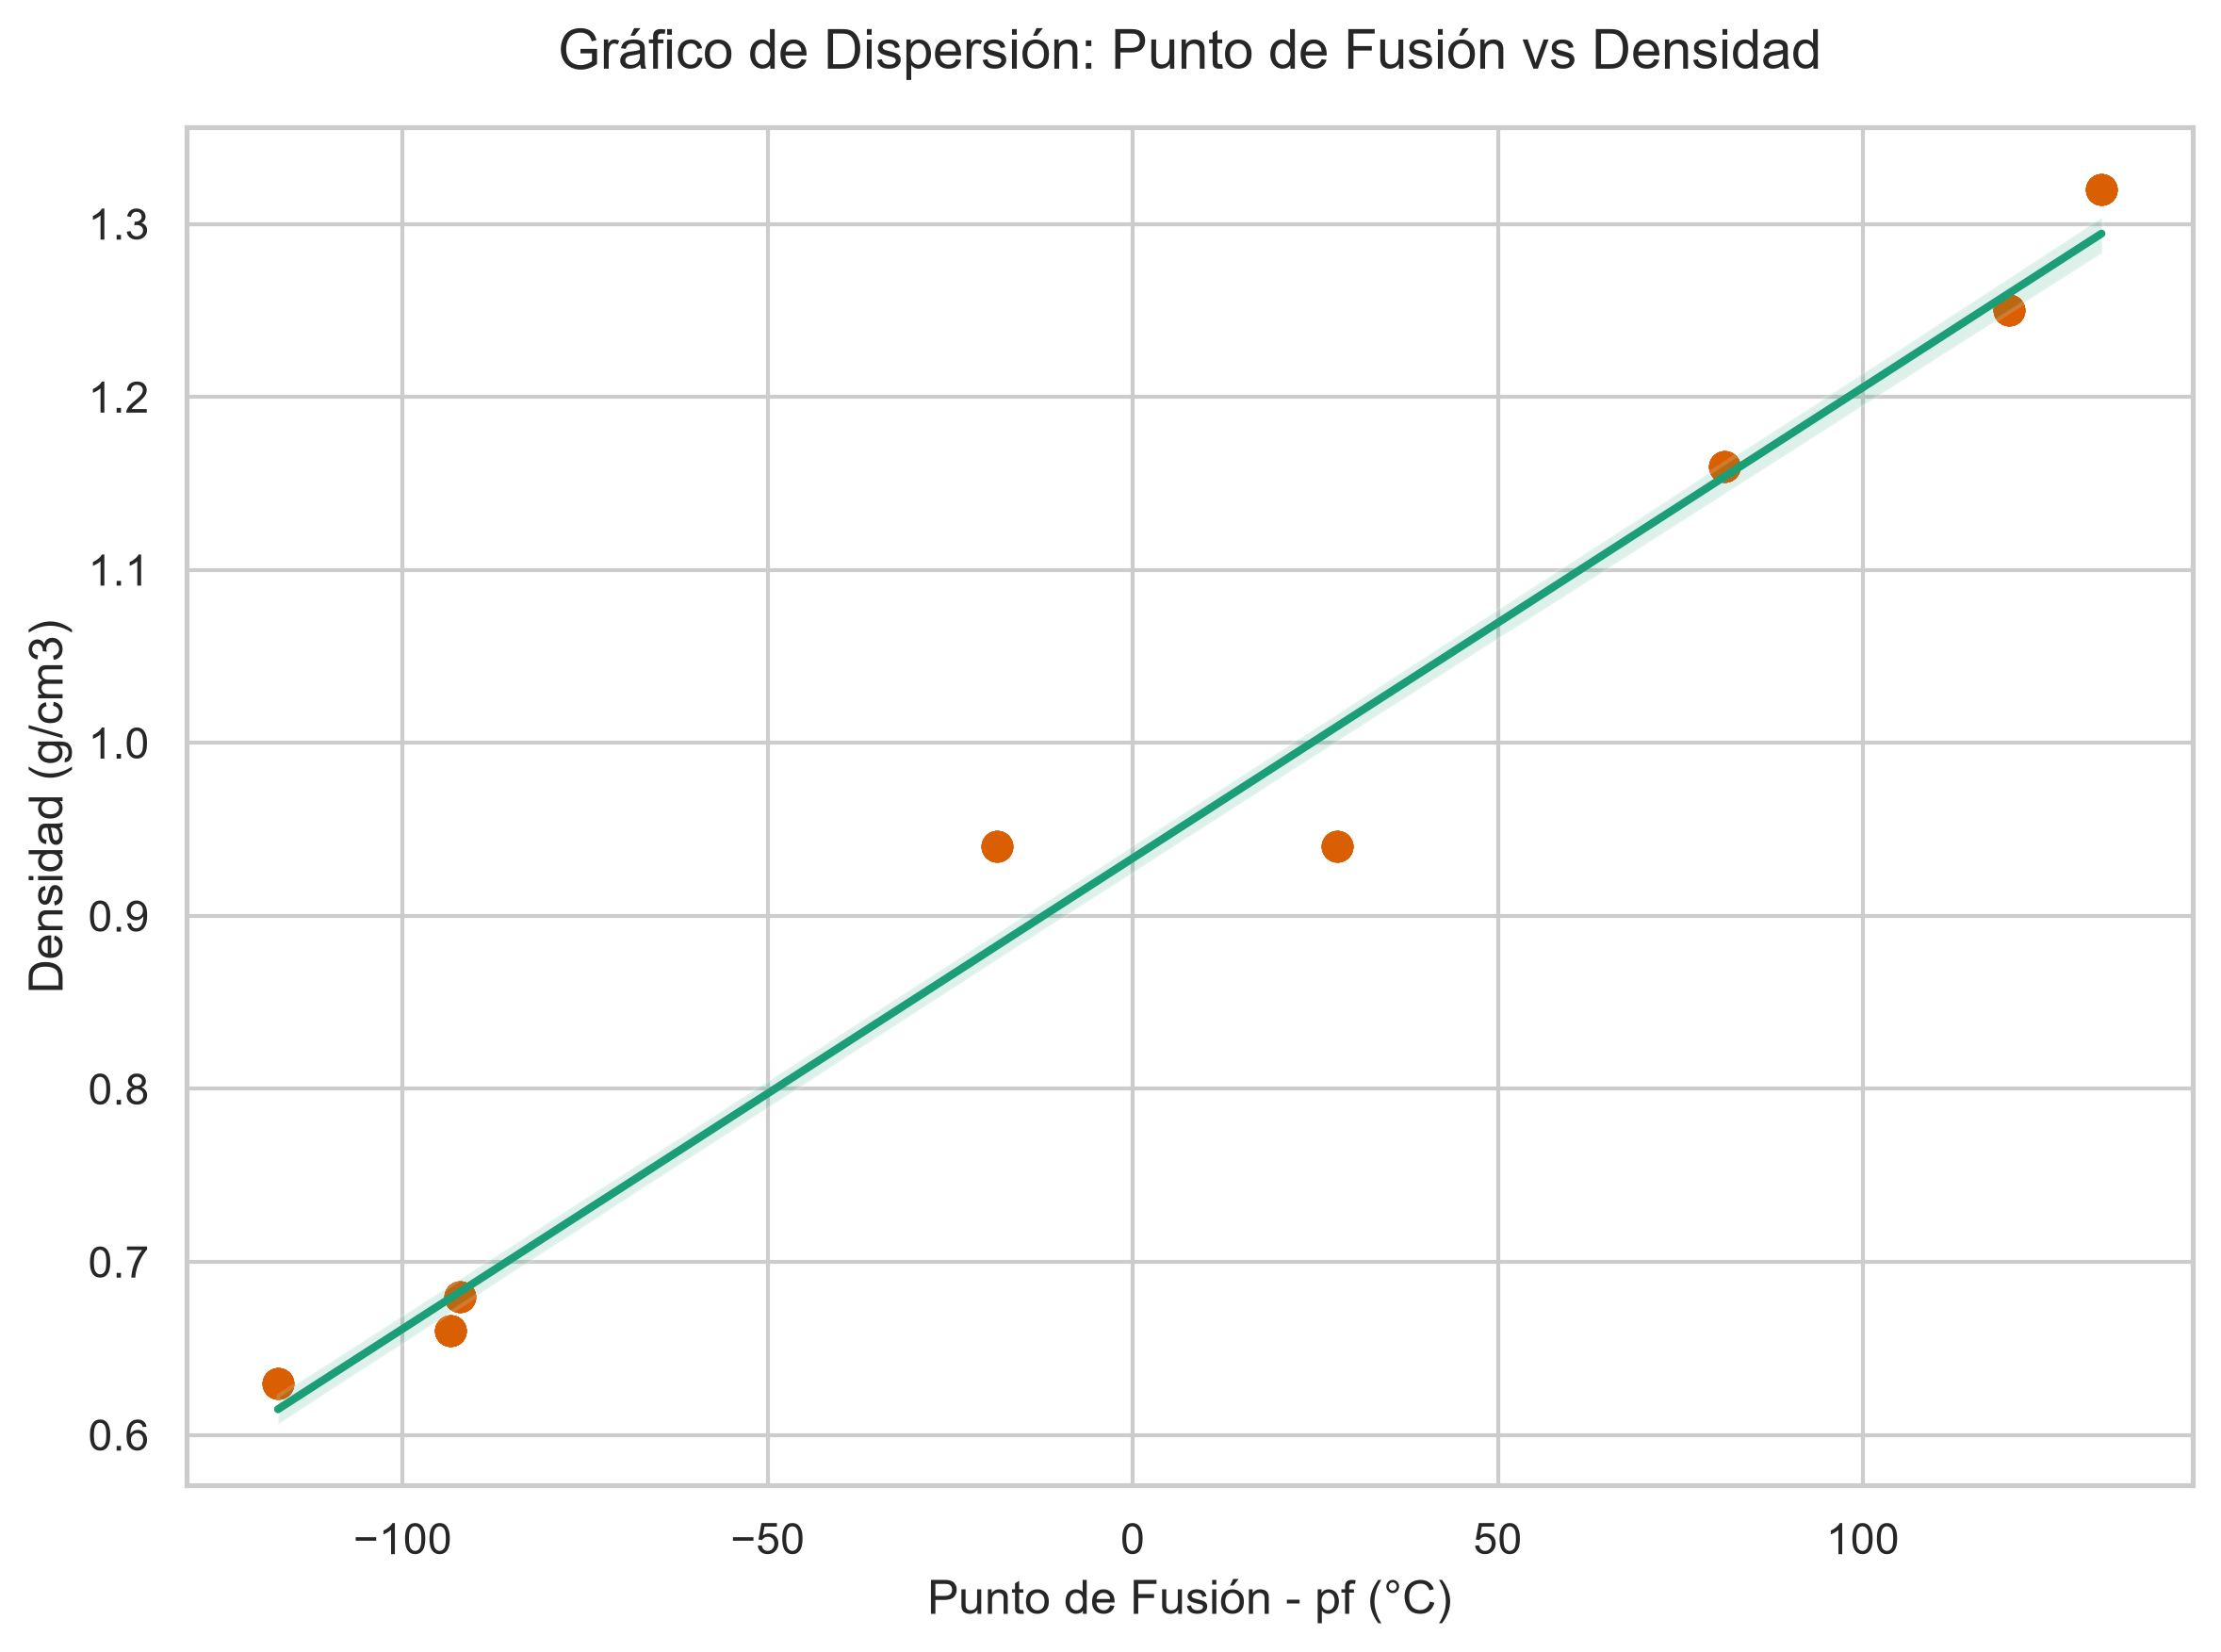
\includegraphics[width=\columnwidth]{03_reg_pf_vs_densidad.png}
	\caption{Punto de fusión frente a densidad.}
	\label{fig:pf-dens}
\end{figure}

\begin{figure}[htbp]
	\centering
	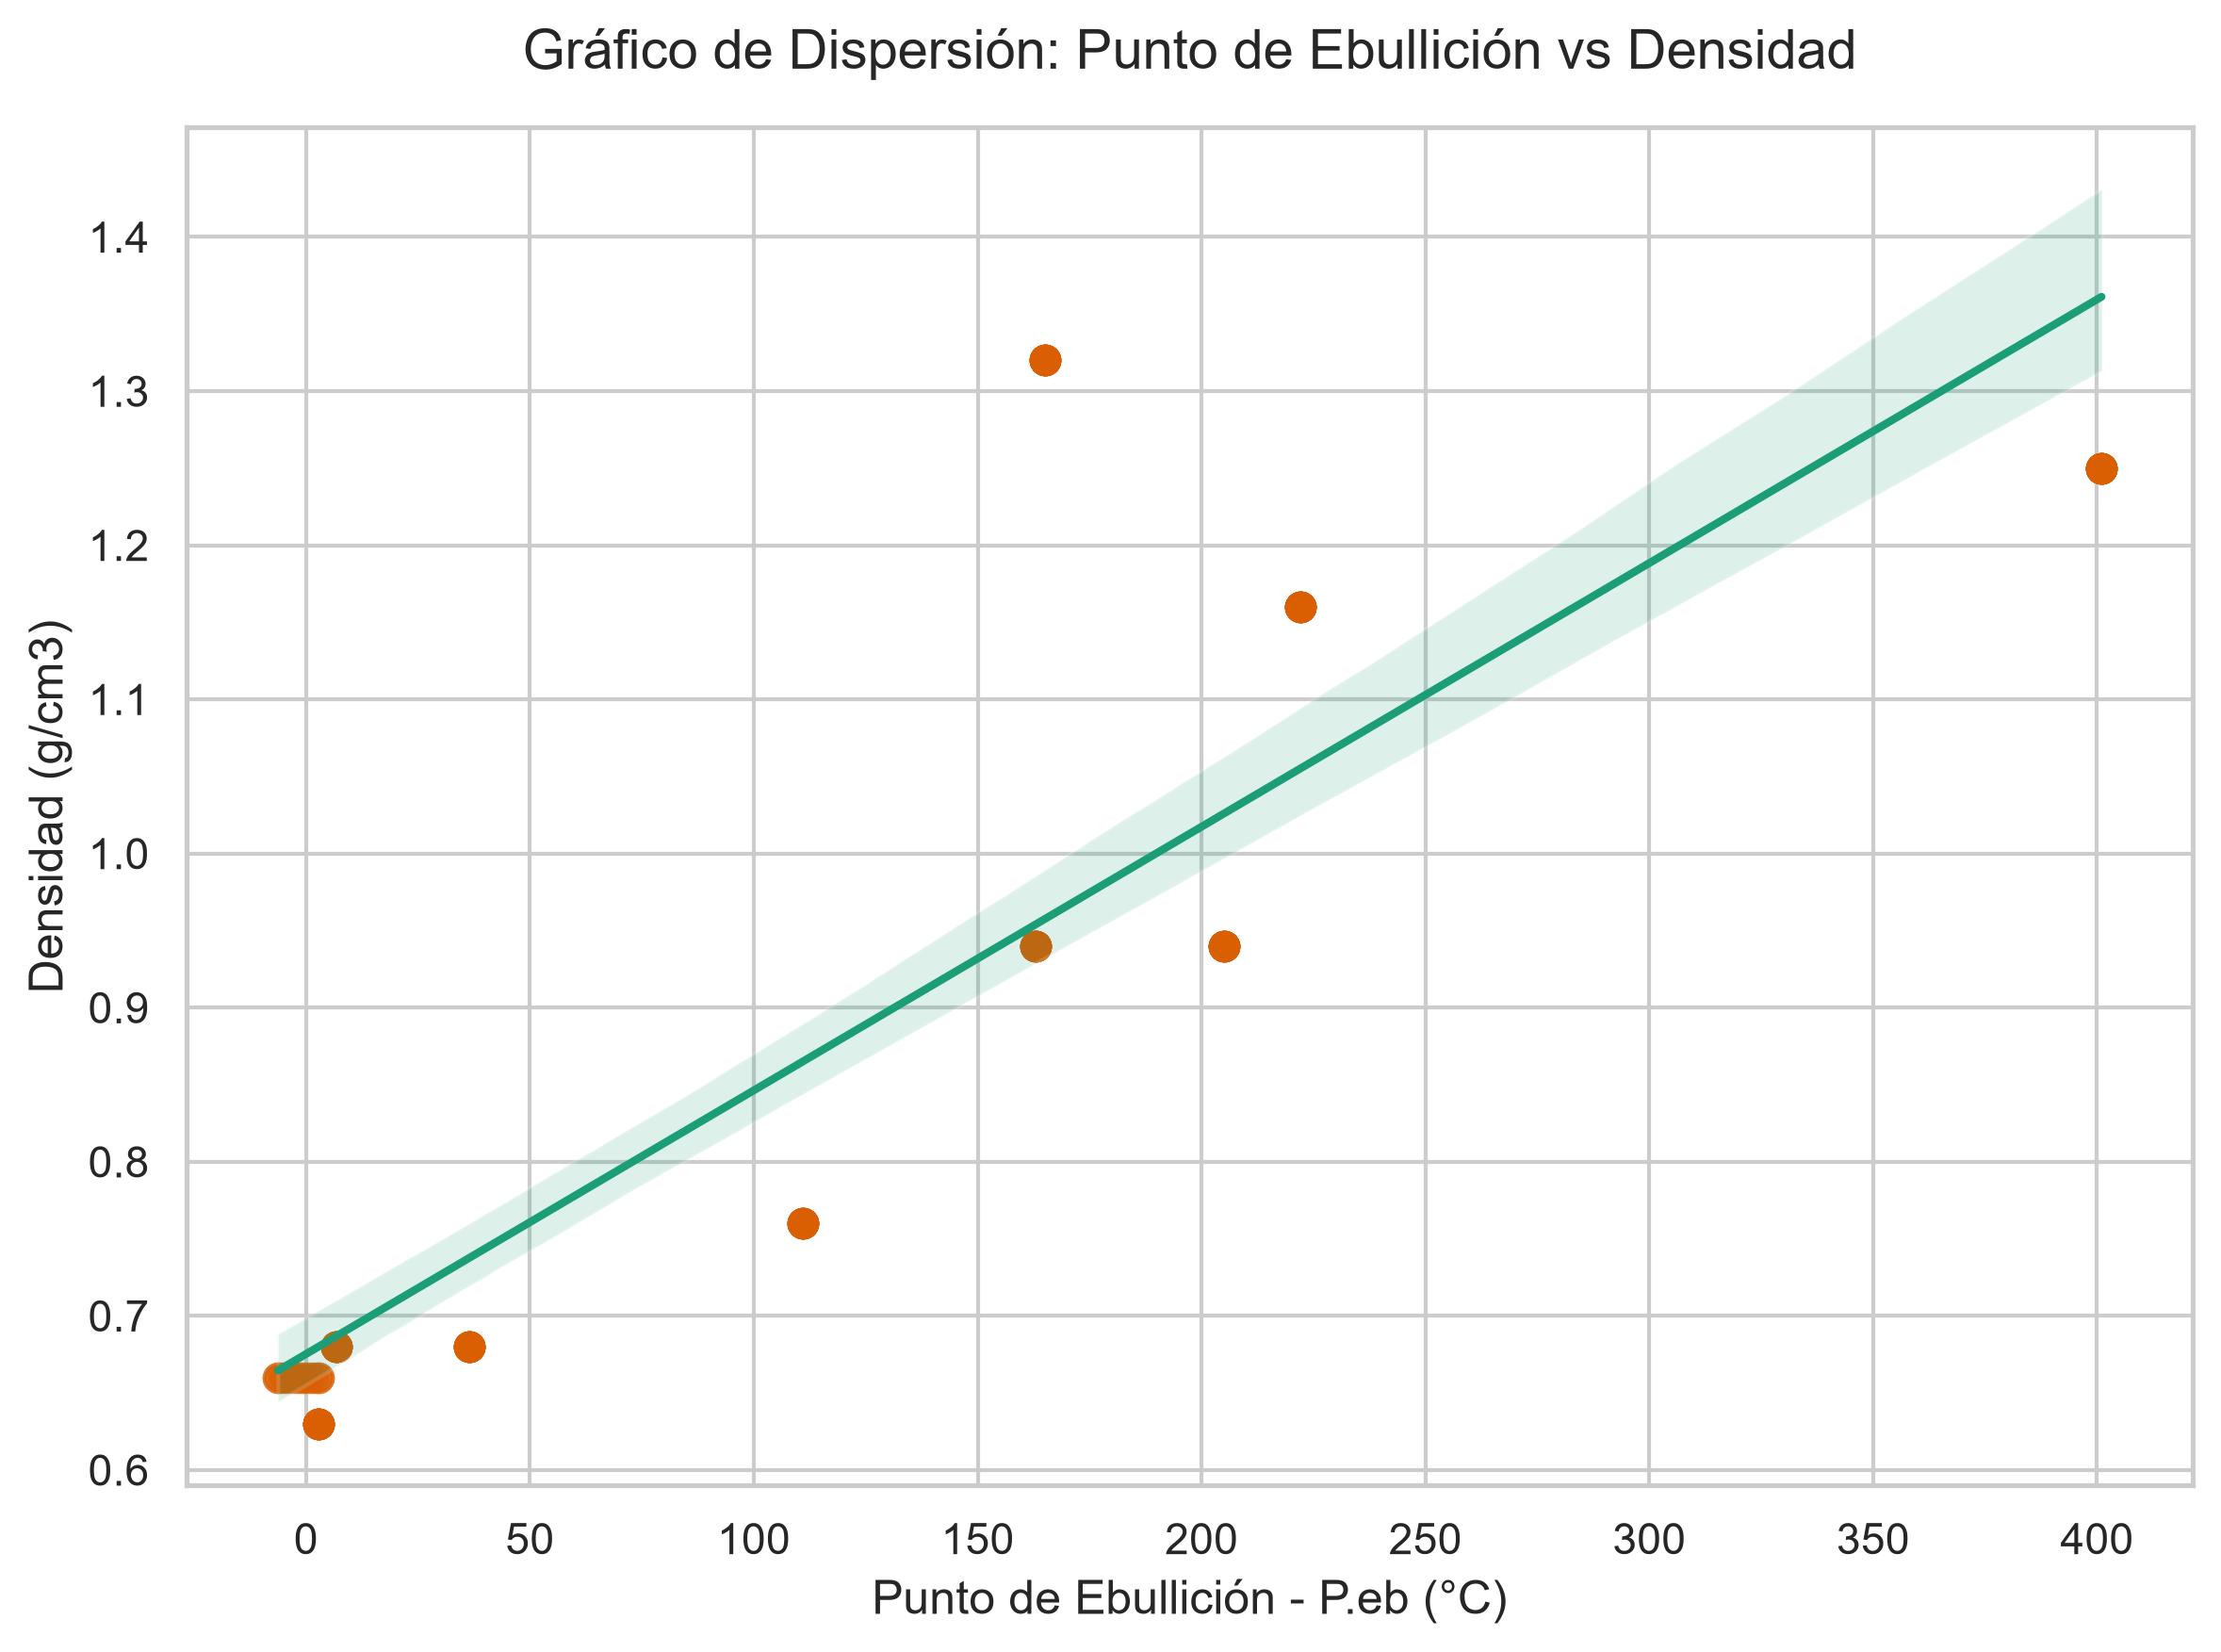
\includegraphics[width=\columnwidth]{04_reg_peb_vs_densidad.png}
	\caption{Punto de ebullición frente a densidad.}
	\label{fig:peb-dens}
\end{figure}

\begin{figure}[htbp]
	\centering
	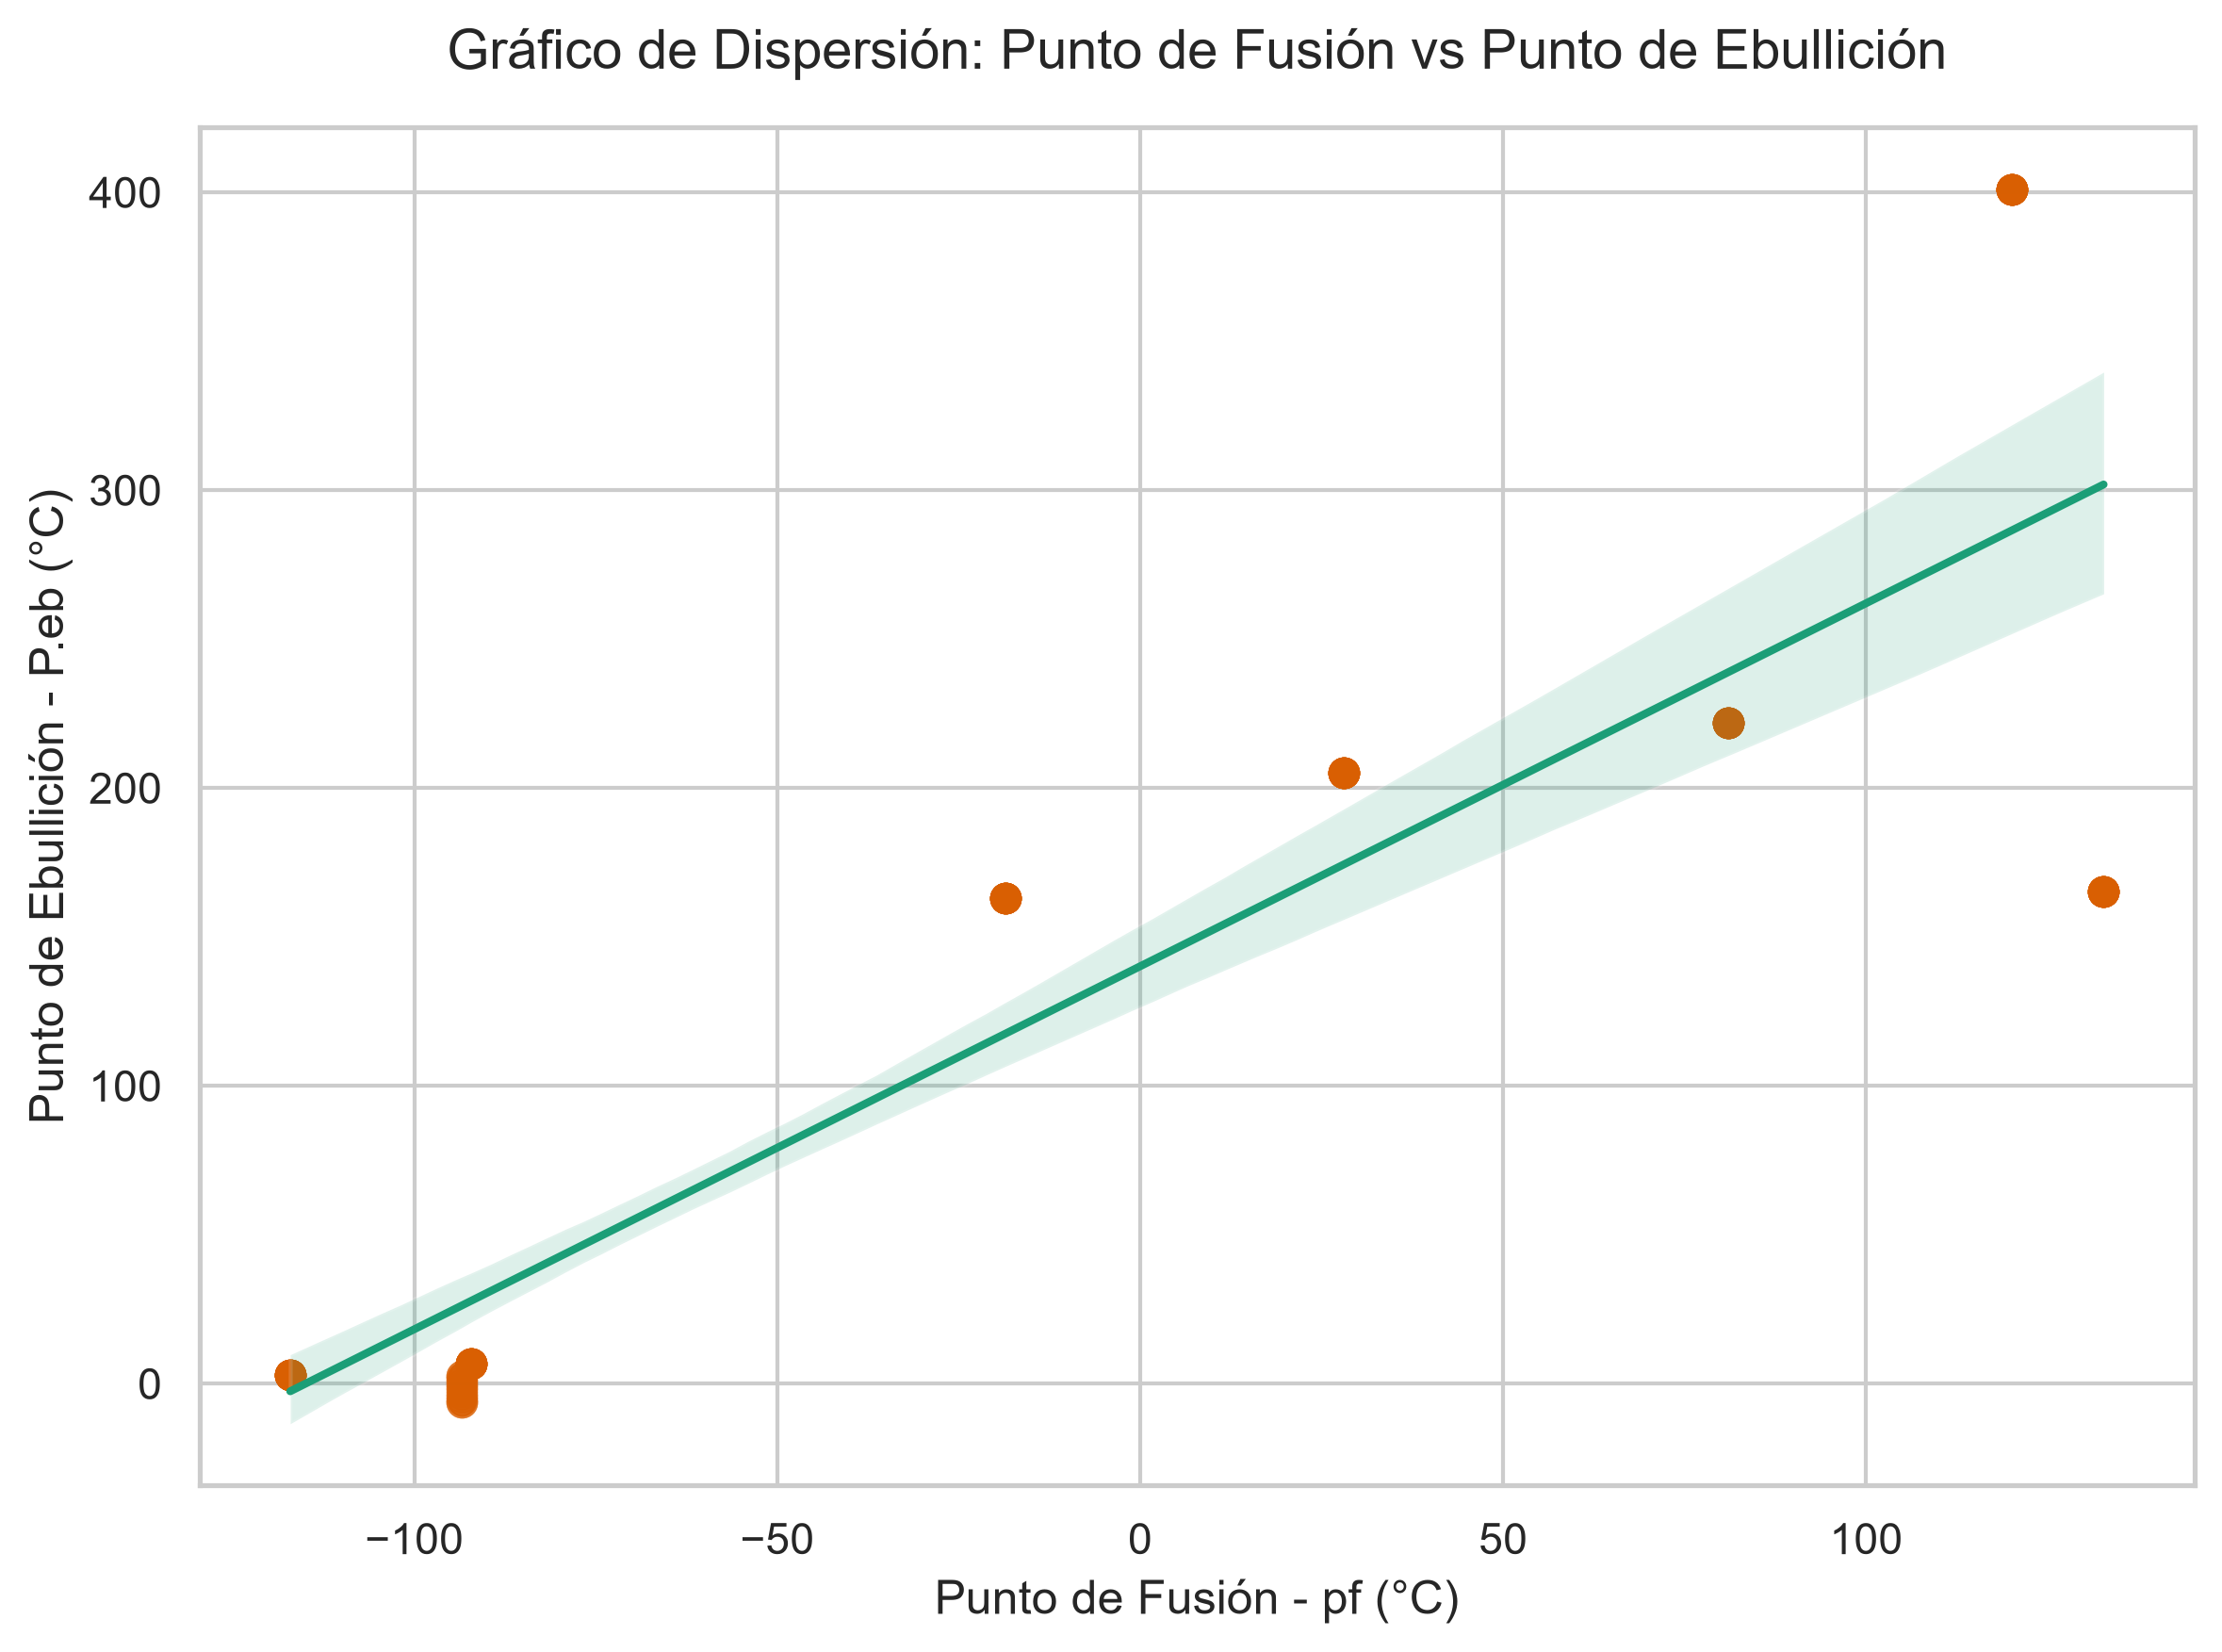
\includegraphics[width=\columnwidth]{05_reg_pf_vs_peb.png}
	\caption{Punto de fusión frente a punto de ebullición.}
	\label{fig:pf-peb}
\end{figure}

\begin{figure}[htbp]
	\centering
	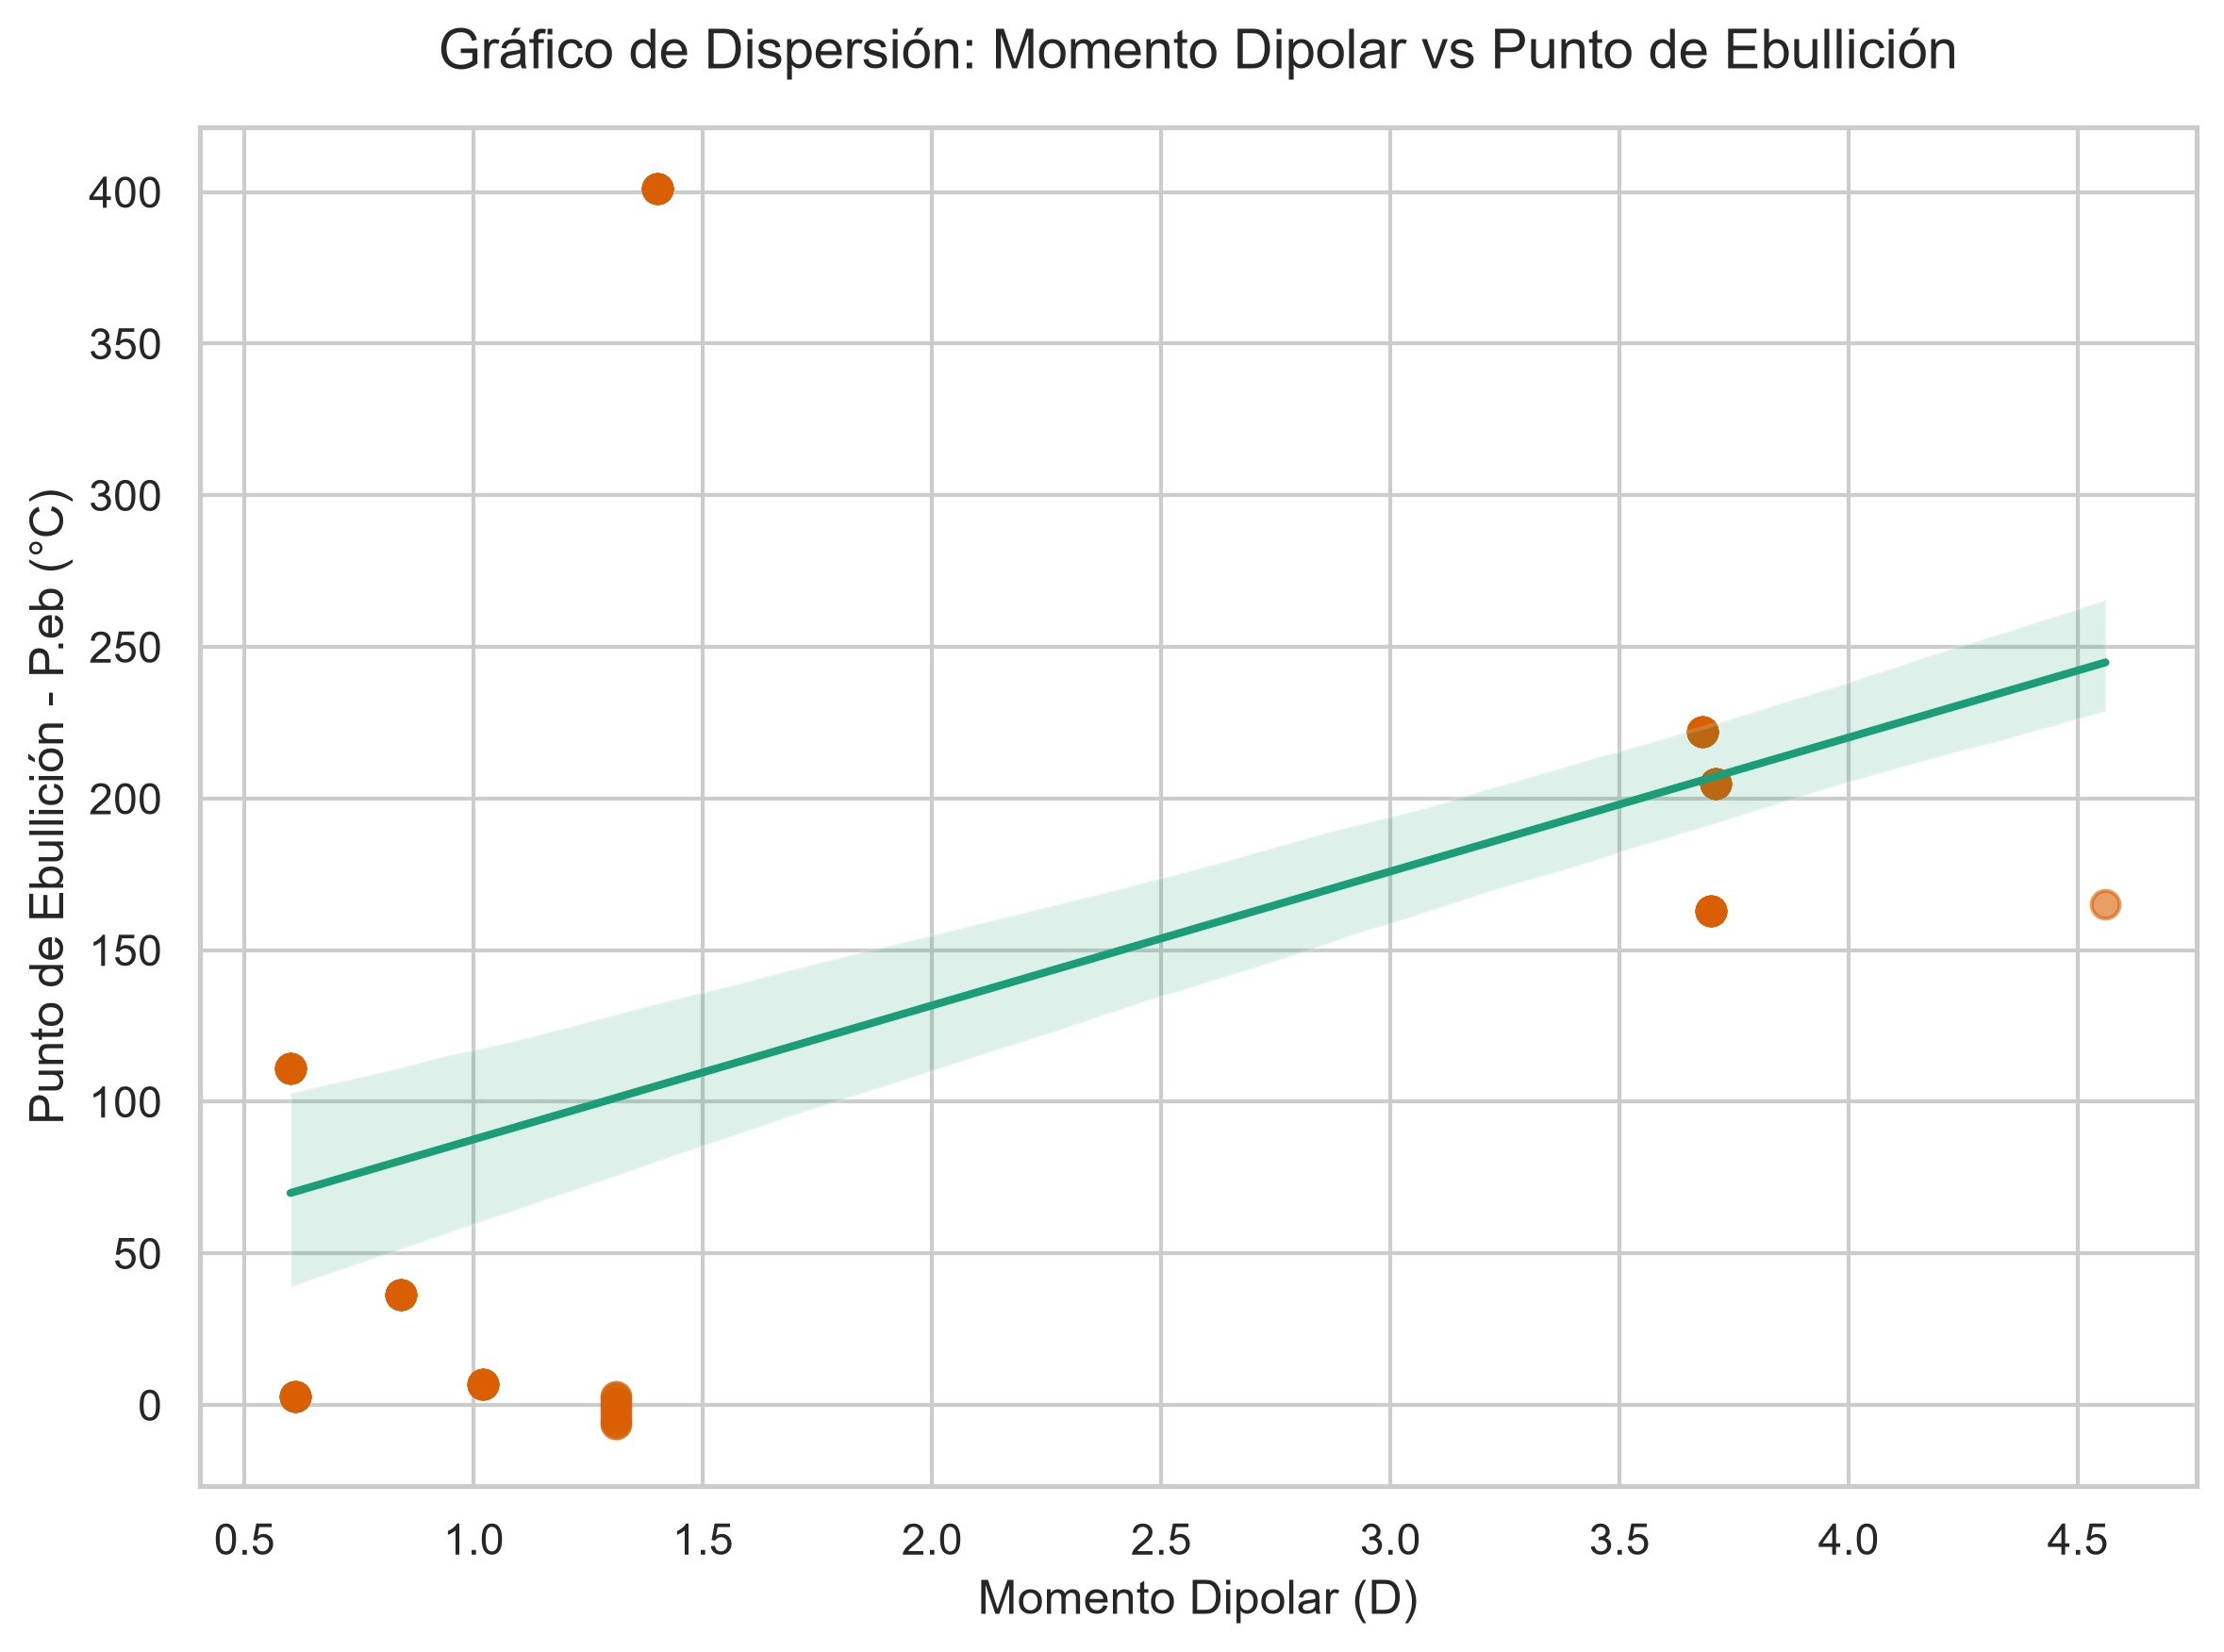
\includegraphics[width=\columnwidth]{06_reg_dipolo_vs_peb.png}
	\caption{Momento dipolar frente a punto de ebullición.}
	\label{fig:dip-peb}
\end{figure}

\subsection{Exploración interactiva con Plotly}
% TODO (Valentina): interpretar; idea central: a igual PM, los compuestos con
% enlace N--H (donadores de puente de H) hierven mucho más alto.
Las Figuras~\ref{fig:burbujas}--\ref{fig:dens-sol} se generaron con Plotly,
una fila por compuesto; sus versiones HTML permiten inspeccionar cada molécula
con el cursor. En la Figura~\ref{fig:burbujas}, trimetilamina
(\SI{2.8}{\degreeCelsius}) y N-metiletanamina (\SI{36.5}{\degreeCelsius}) tienen
el mismo peso molecular (\SI{59.11}{\gram\per\mole}): la diferencia se debe a que
sólo la segunda posee enlace N--H y forma puentes de hidrógeno.
\textit{[Interpretación pendiente.]}

\begin{figure}[htbp]
	\centering
	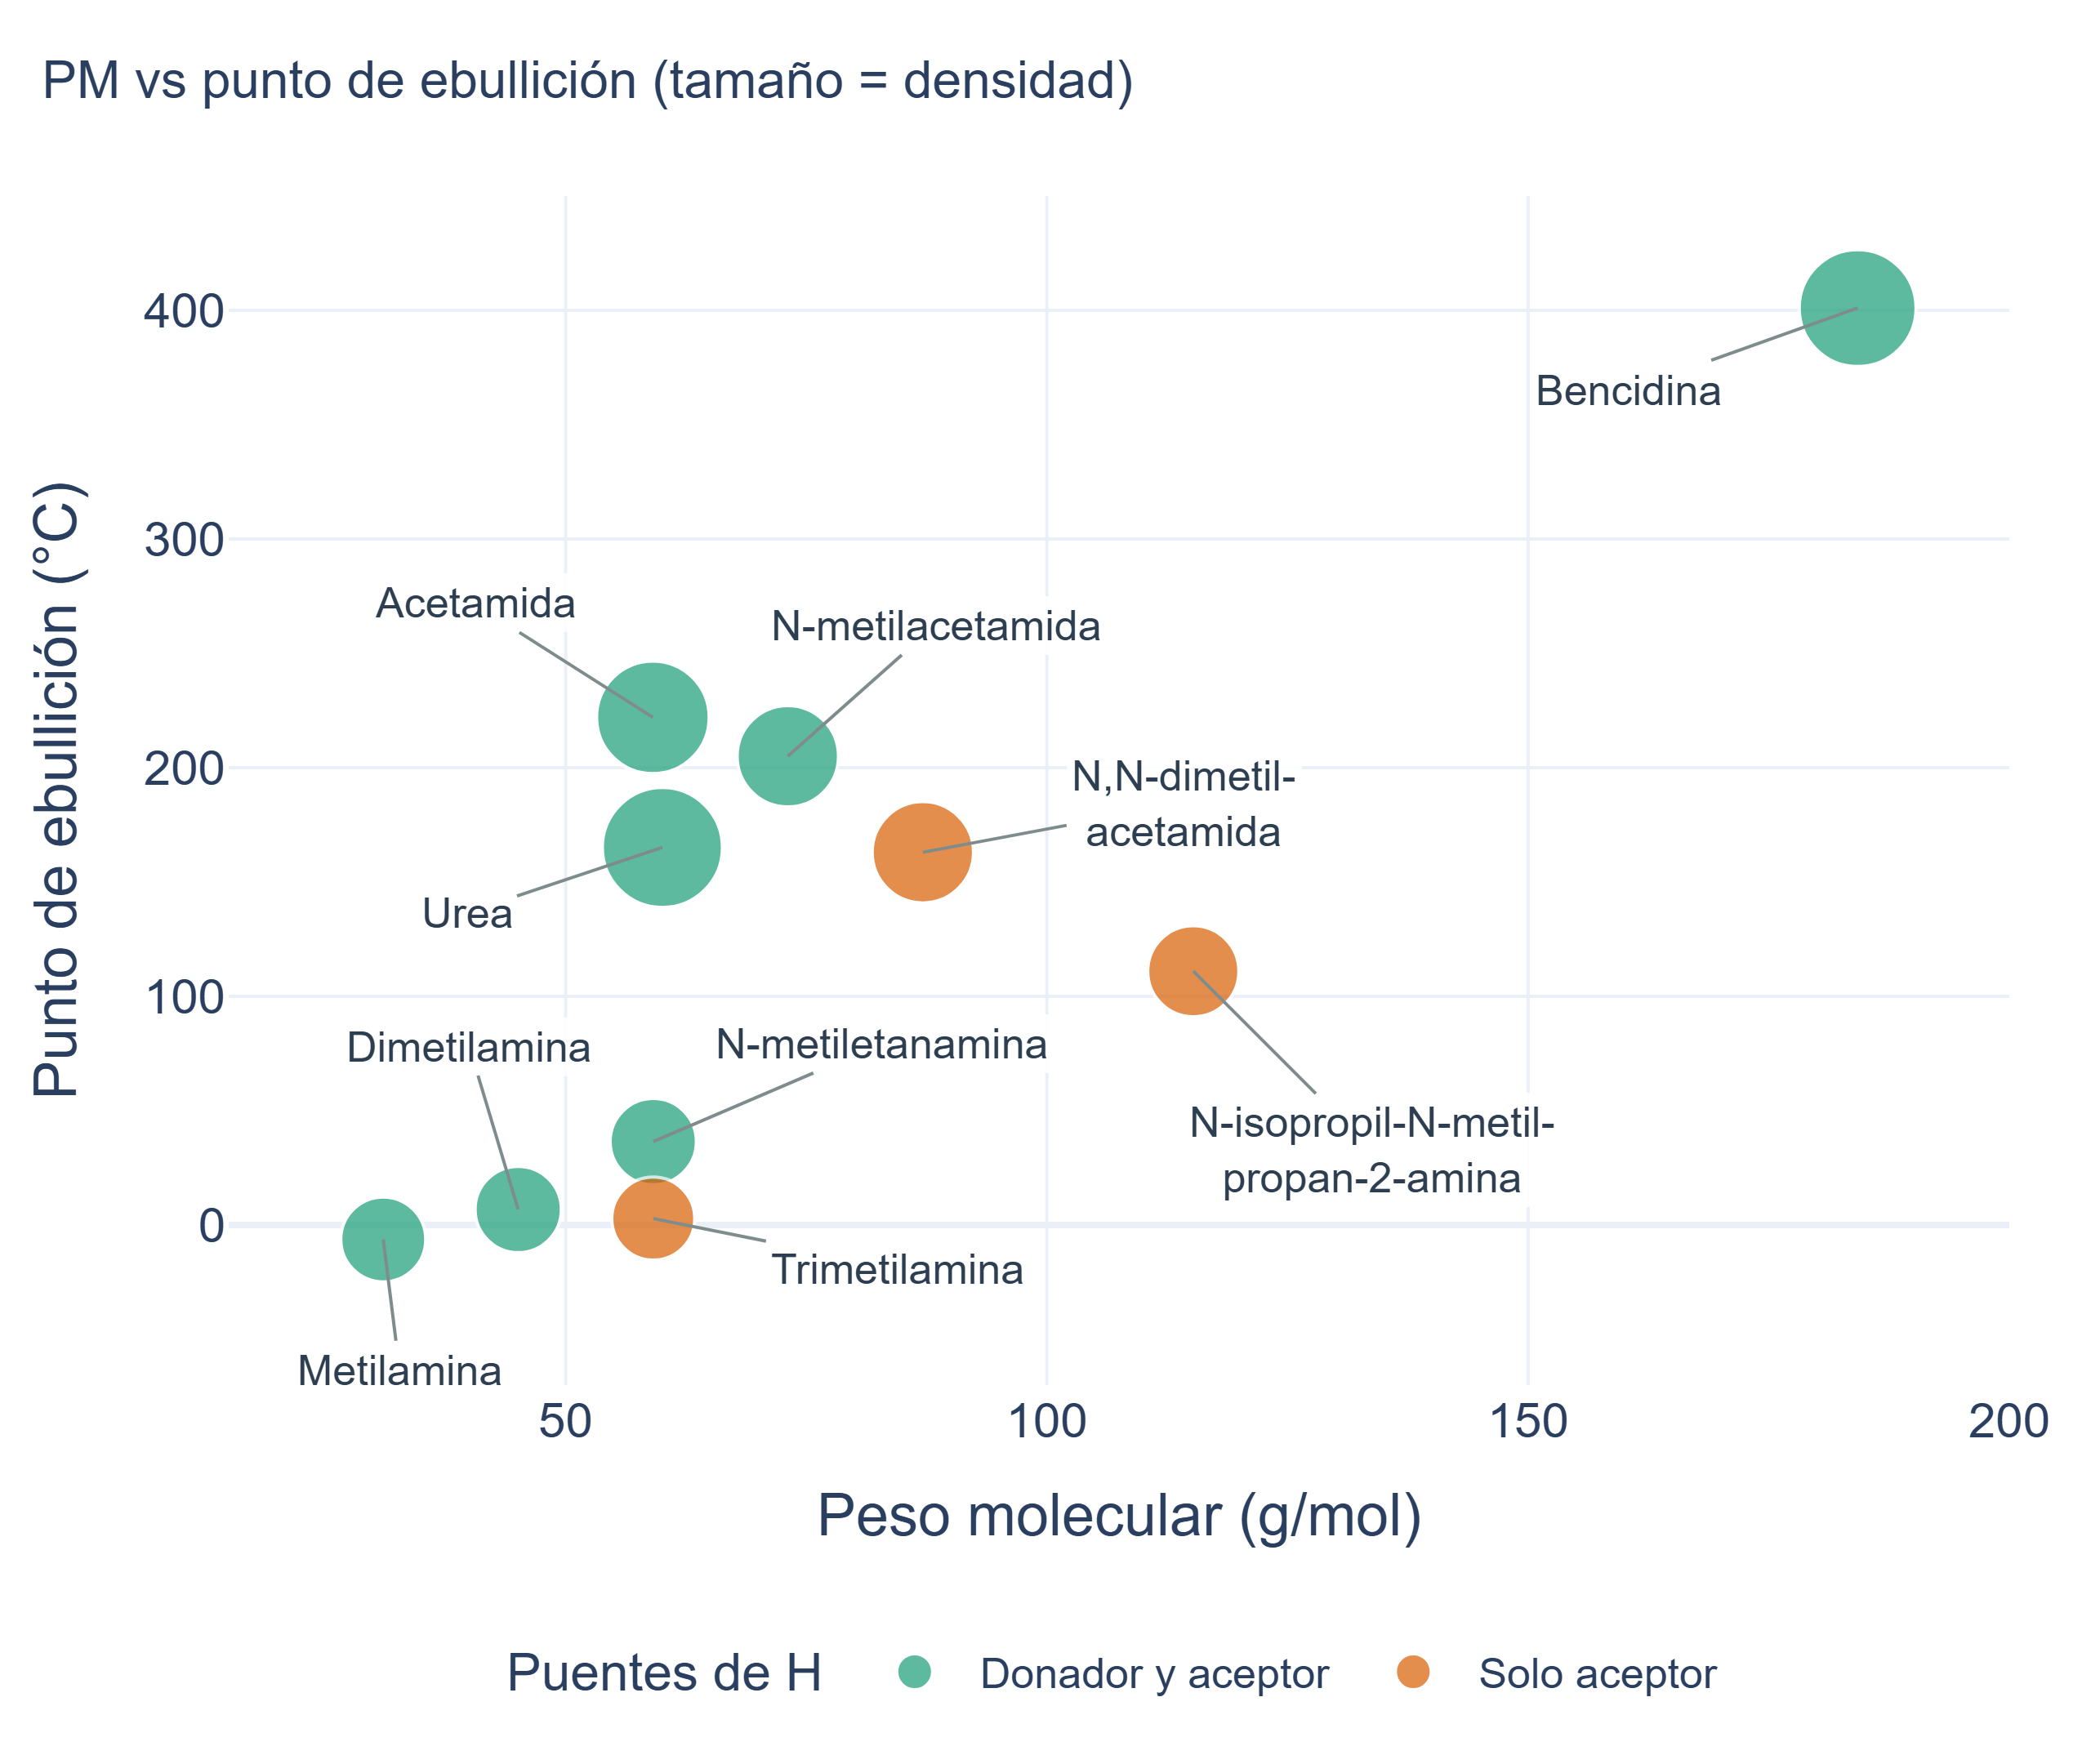
\includegraphics[width=\columnwidth]{11_plotly_burbujas_pm_peb.png}
	\caption{Peso molecular frente a punto de ebullición; el tamaño representa la densidad y el color la capacidad de formar puentes de hidrógeno.}
	\label{fig:burbujas}
\end{figure}

\begin{figure}[htbp]
	\centering
	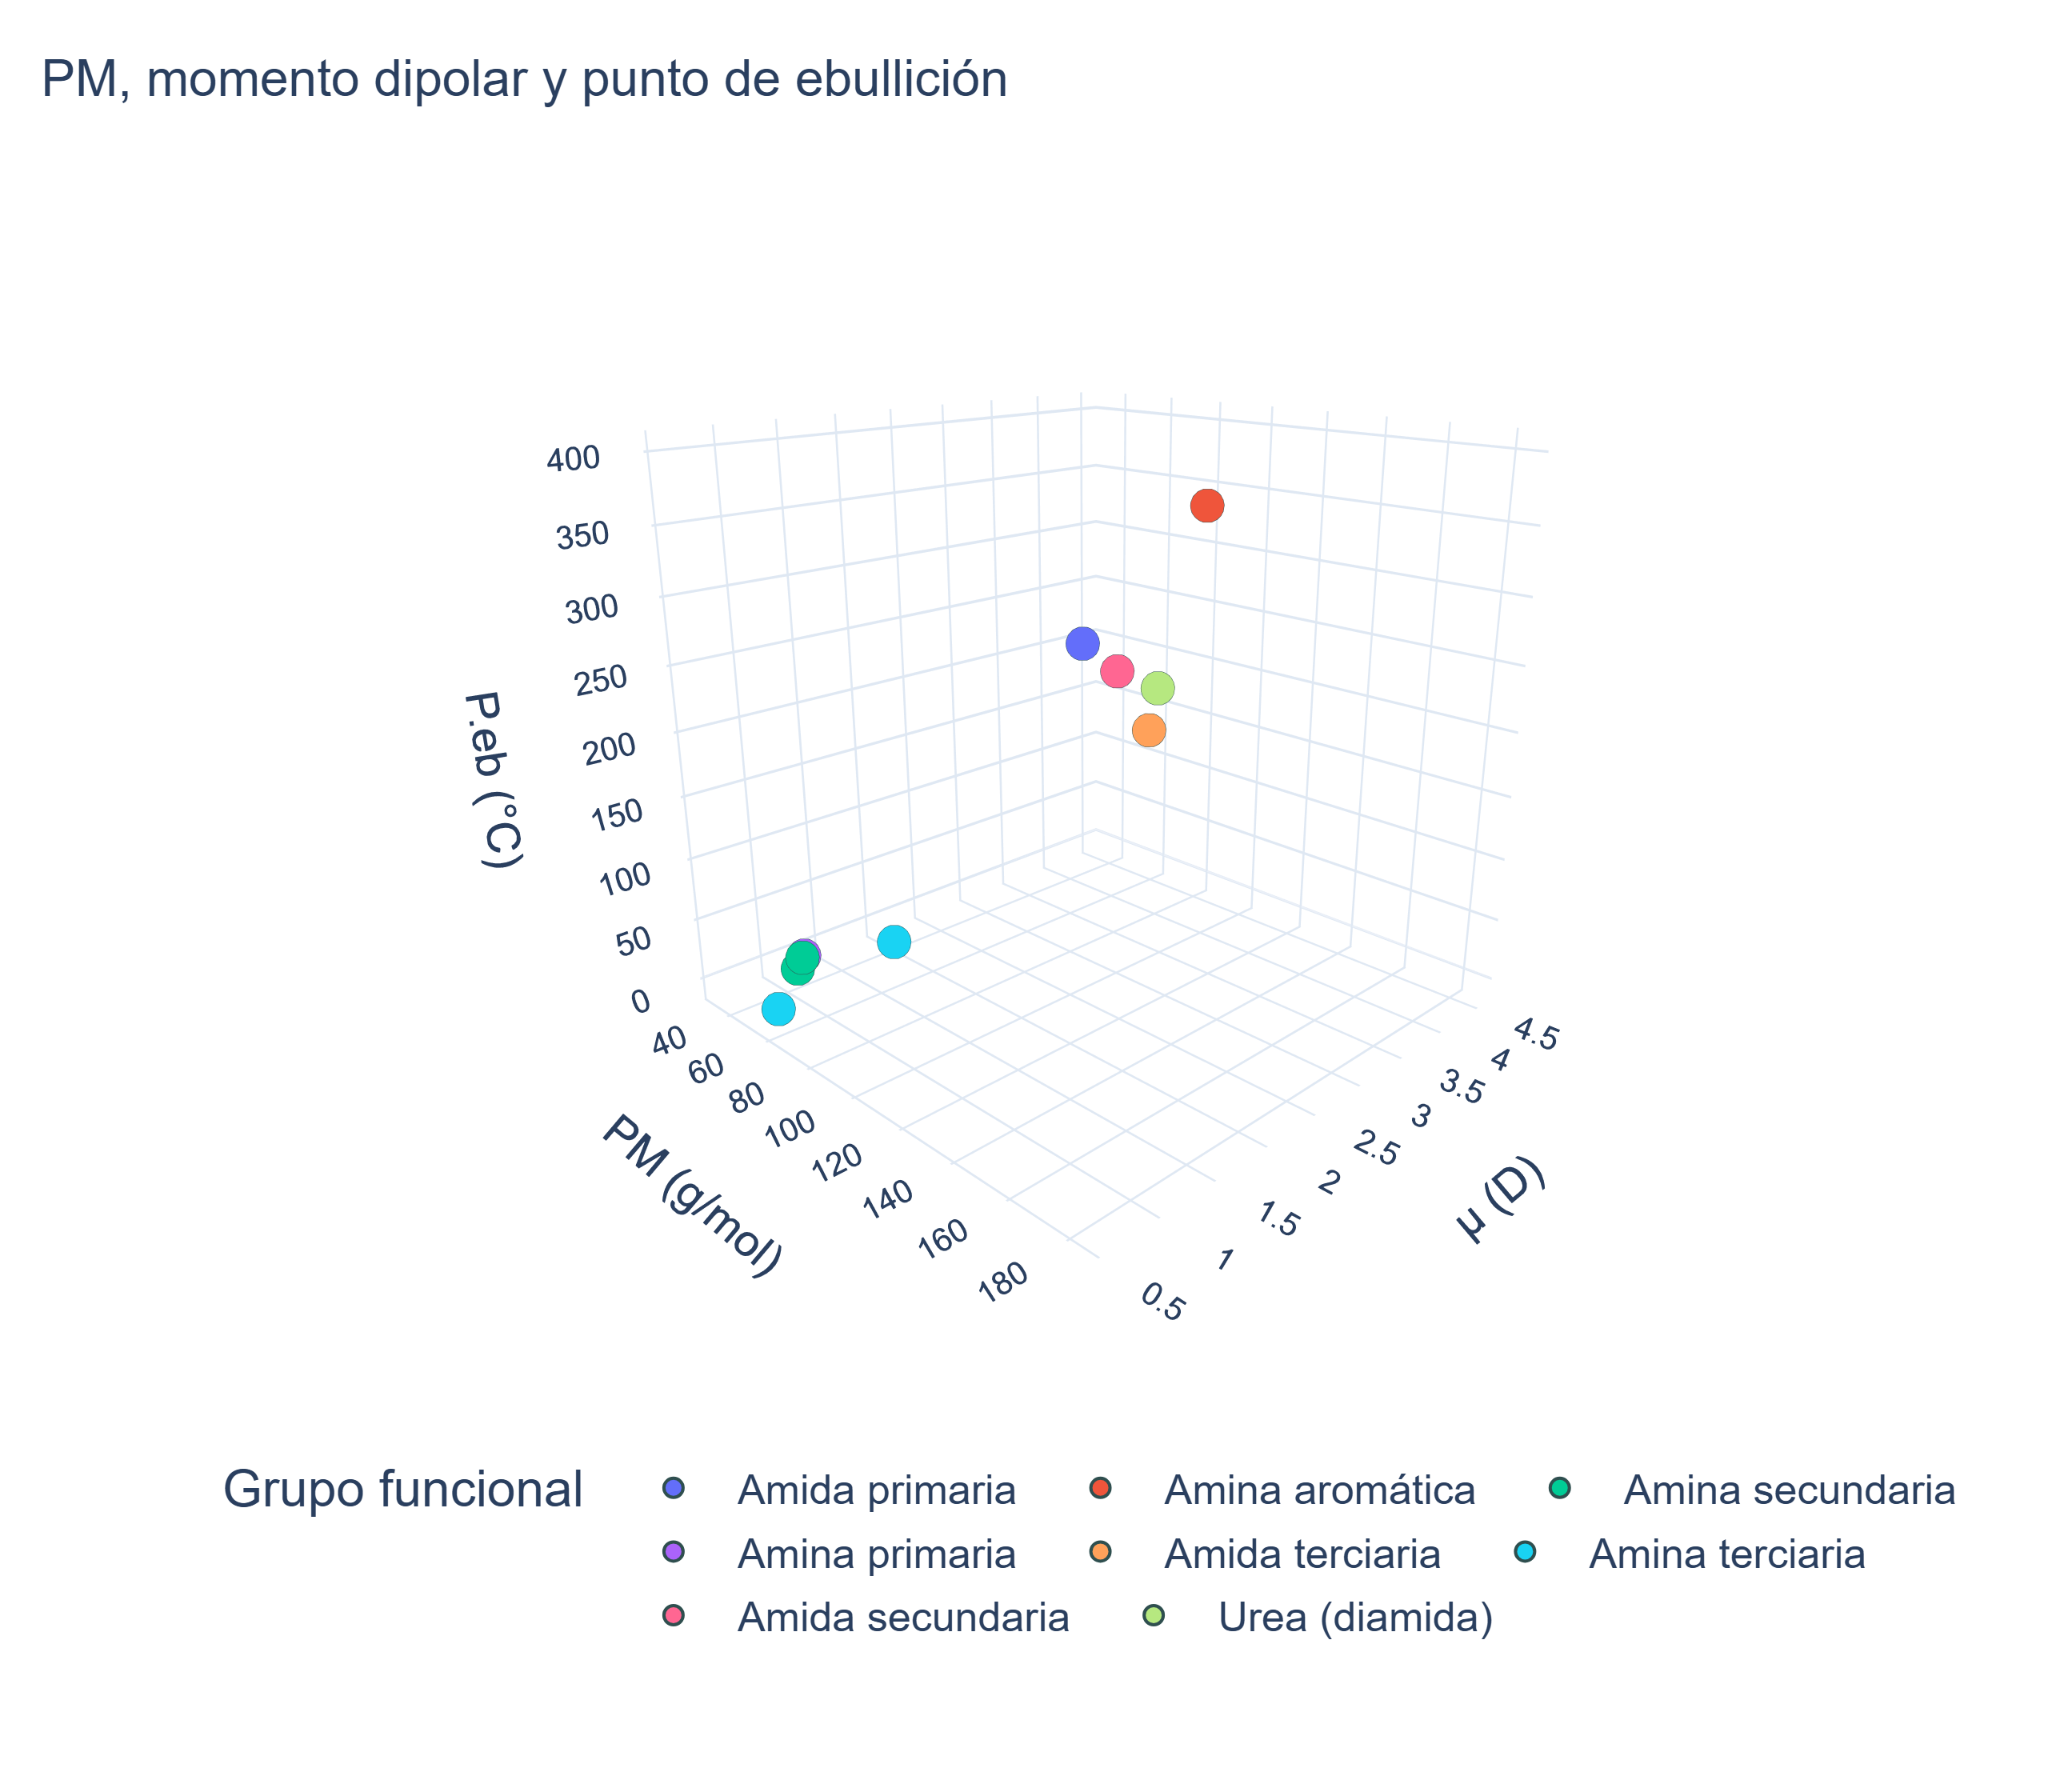
\includegraphics[width=\columnwidth]{12_plotly_3d_pm_dipolo_peb.png}
	\caption{Espacio tridimensional de peso molecular, momento dipolar y punto de ebullición por grupo funcional.}
	\label{fig:3d}
\end{figure}

\begin{figure}[htbp]
	\centering
	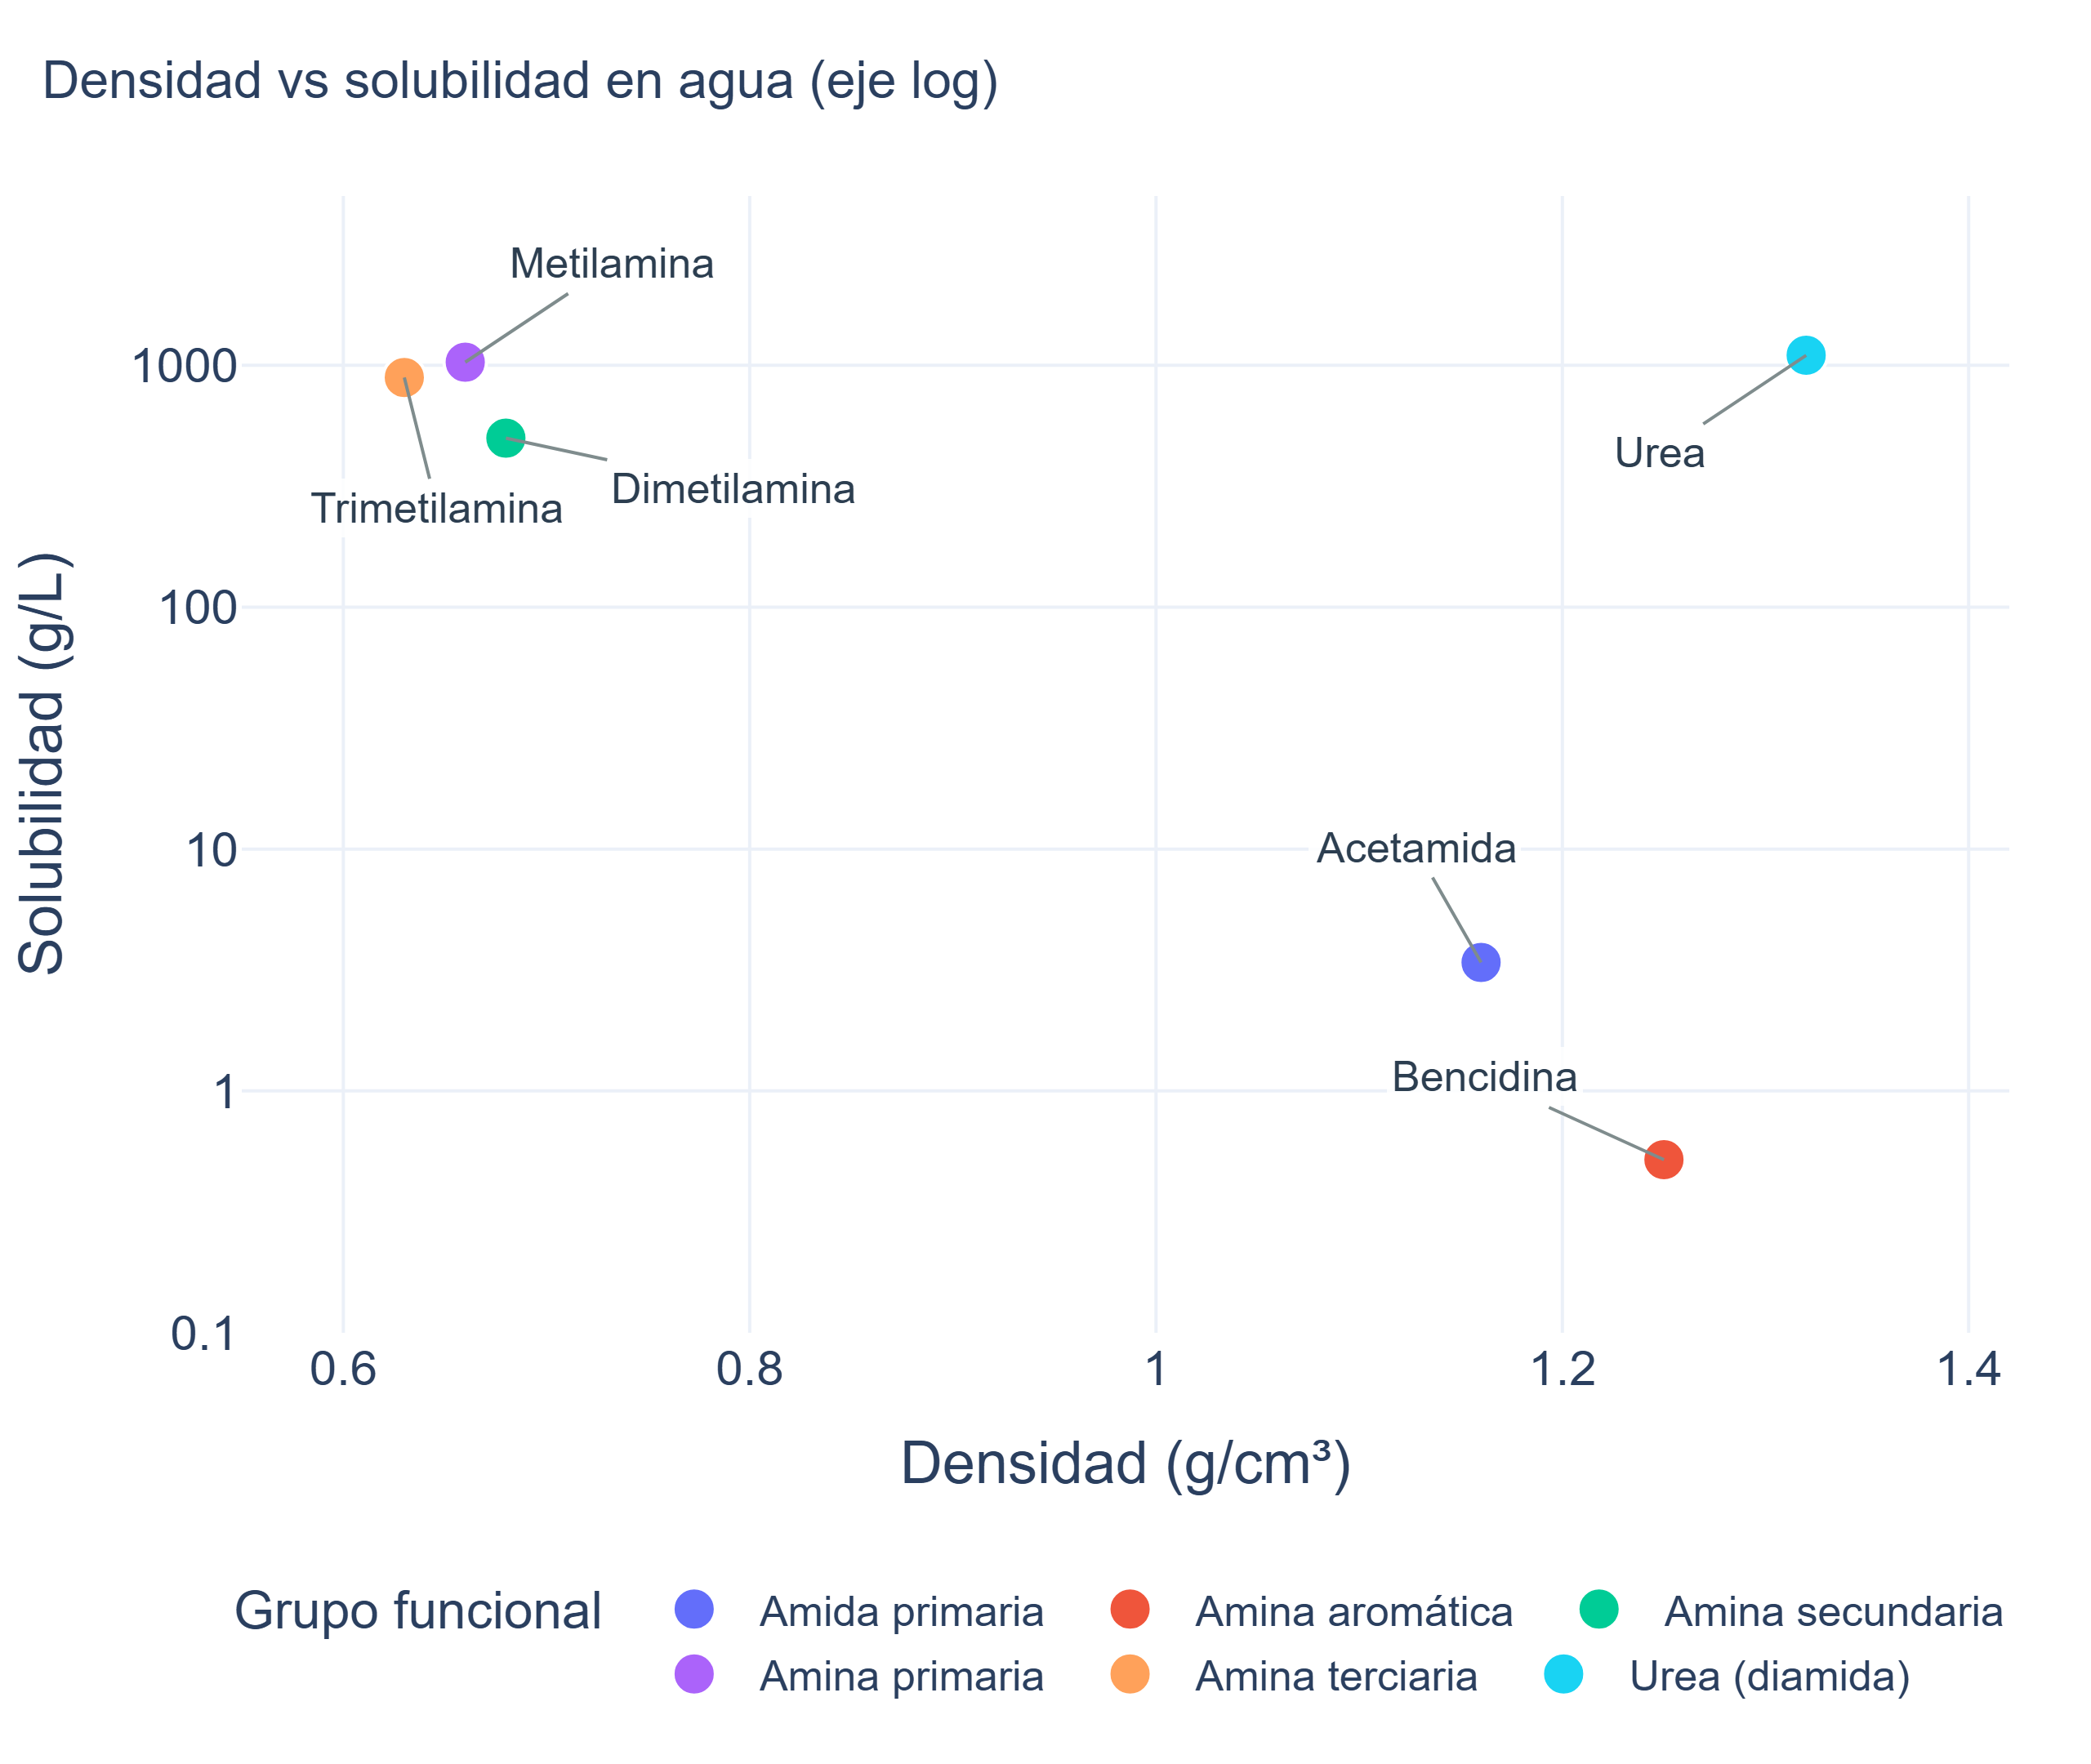
\includegraphics[width=\columnwidth]{13_plotly_densidad_solubilidad.png}
	\caption{Densidad frente a solubilidad en agua (eje logarítmico).}
	\label{fig:dens-sol}
\end{figure}

\subsection{Distribución por tipo de reacción y medio}
% TODO (Valentina): explicar qué representa TR y comparar medianas/dispersiones.
La Figura~\ref{fig:frecuencias} compara la frecuencia de cada mecanismo de
reacción y de cada medio; la sustitución nucleofílica (SN) domina, coherente con
el carácter nucleófilo del par libre del nitrógeno. Las
Figuras~\ref{fig:violin}--\ref{fig:dona} describen la distribución de
probabilidad de TR según el tipo de reacción y el medio.
\textit{[Interpretación pendiente.]}

\begin{figure}[htbp]
	\centering
	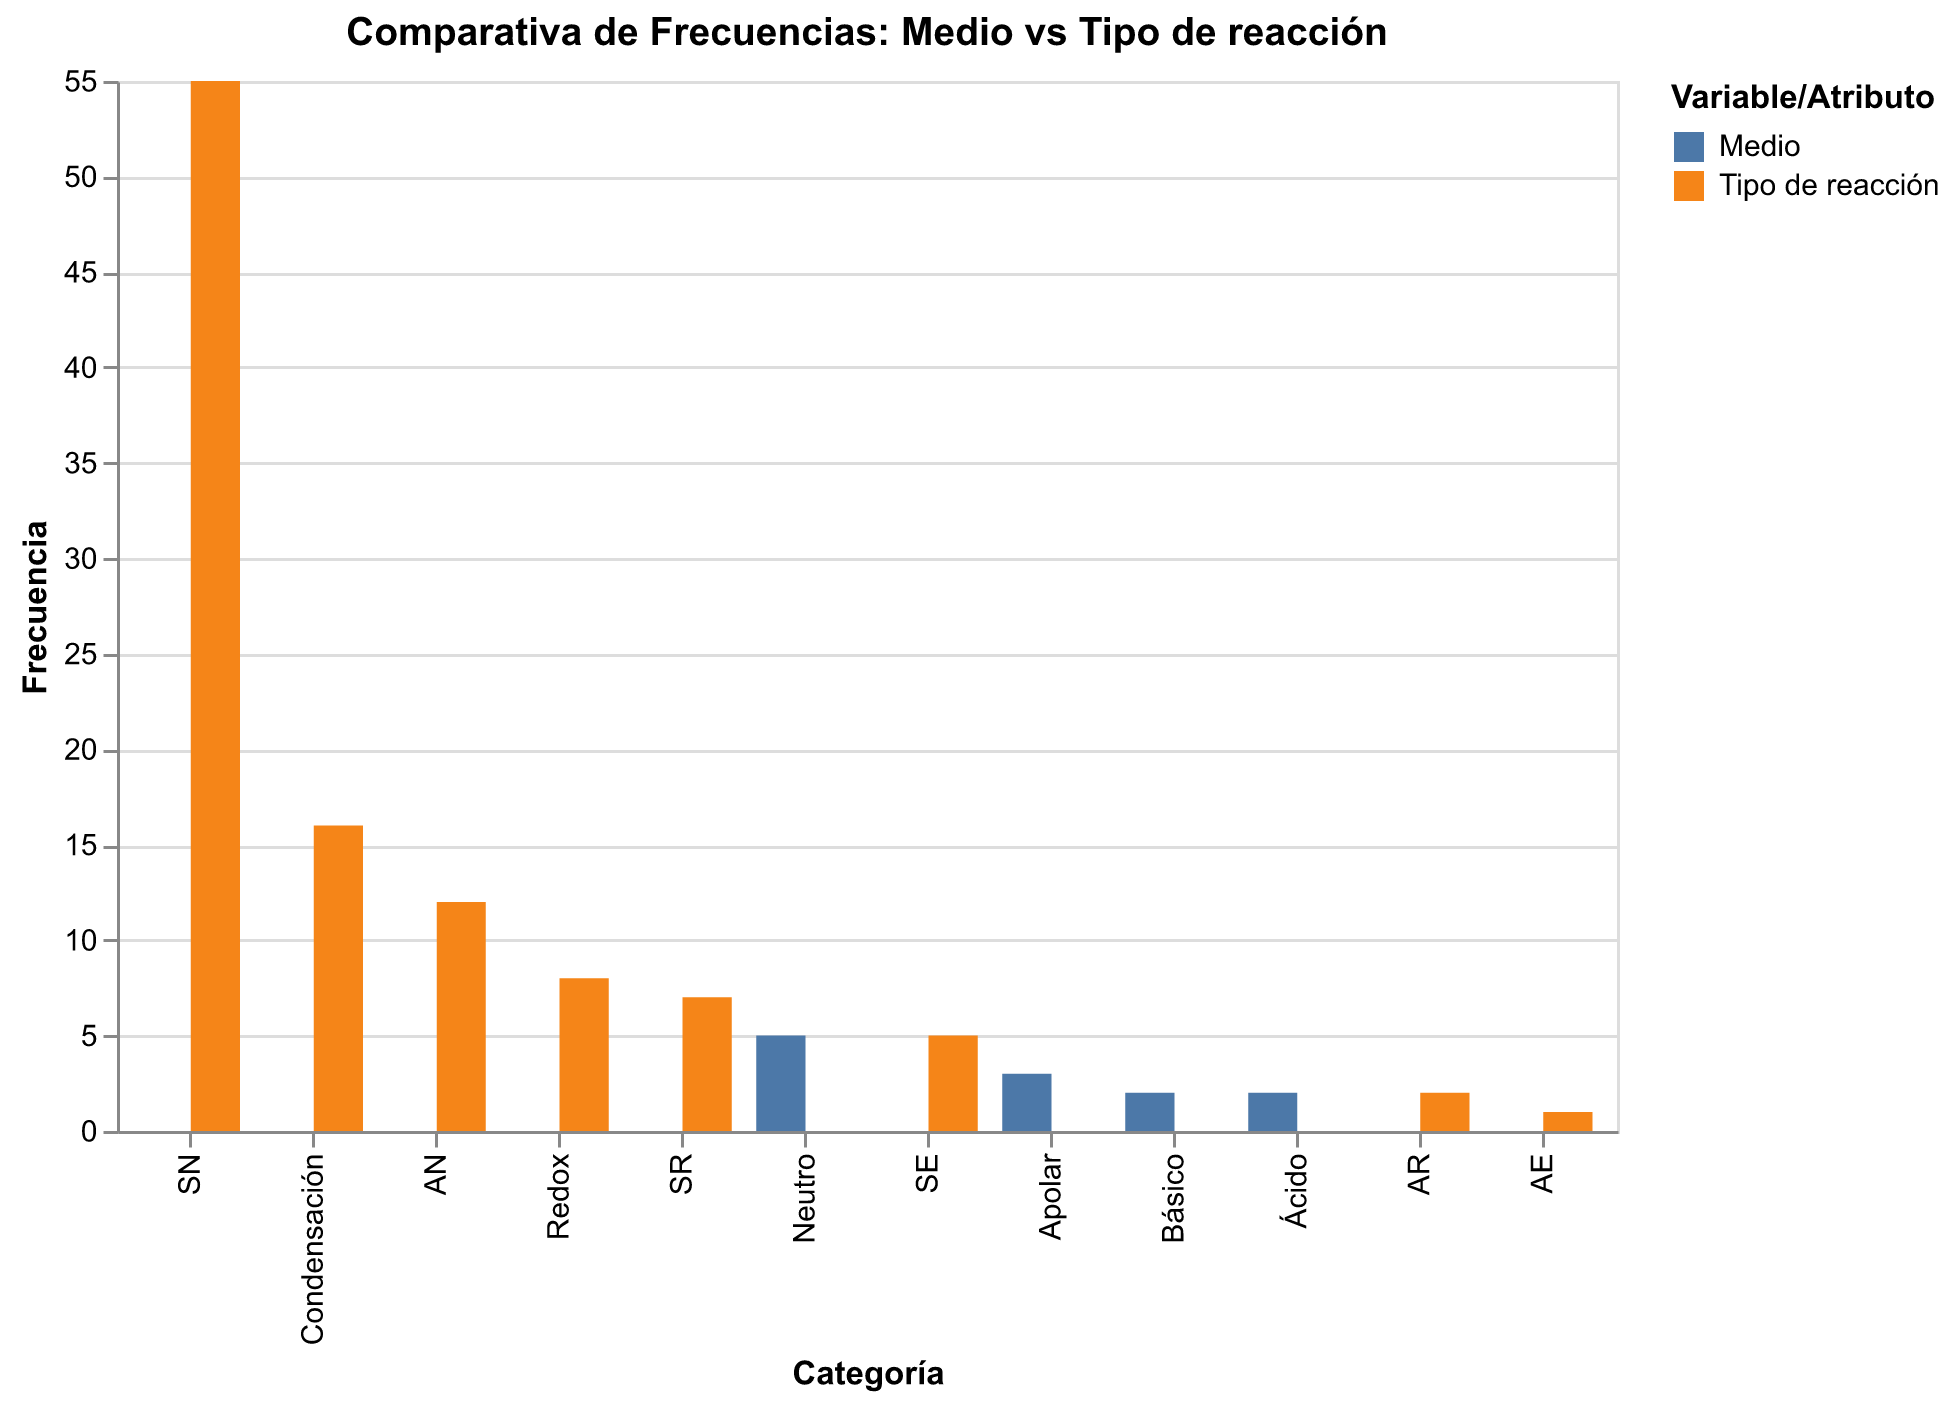
\includegraphics[width=\columnwidth]{09_frecuencias_medio_tipo.png}
	\caption{Frecuencia de los tipos de reacción y de los medios reportados.}
	\label{fig:frecuencias}
\end{figure}

\begin{figure}[htbp]
	\centering
	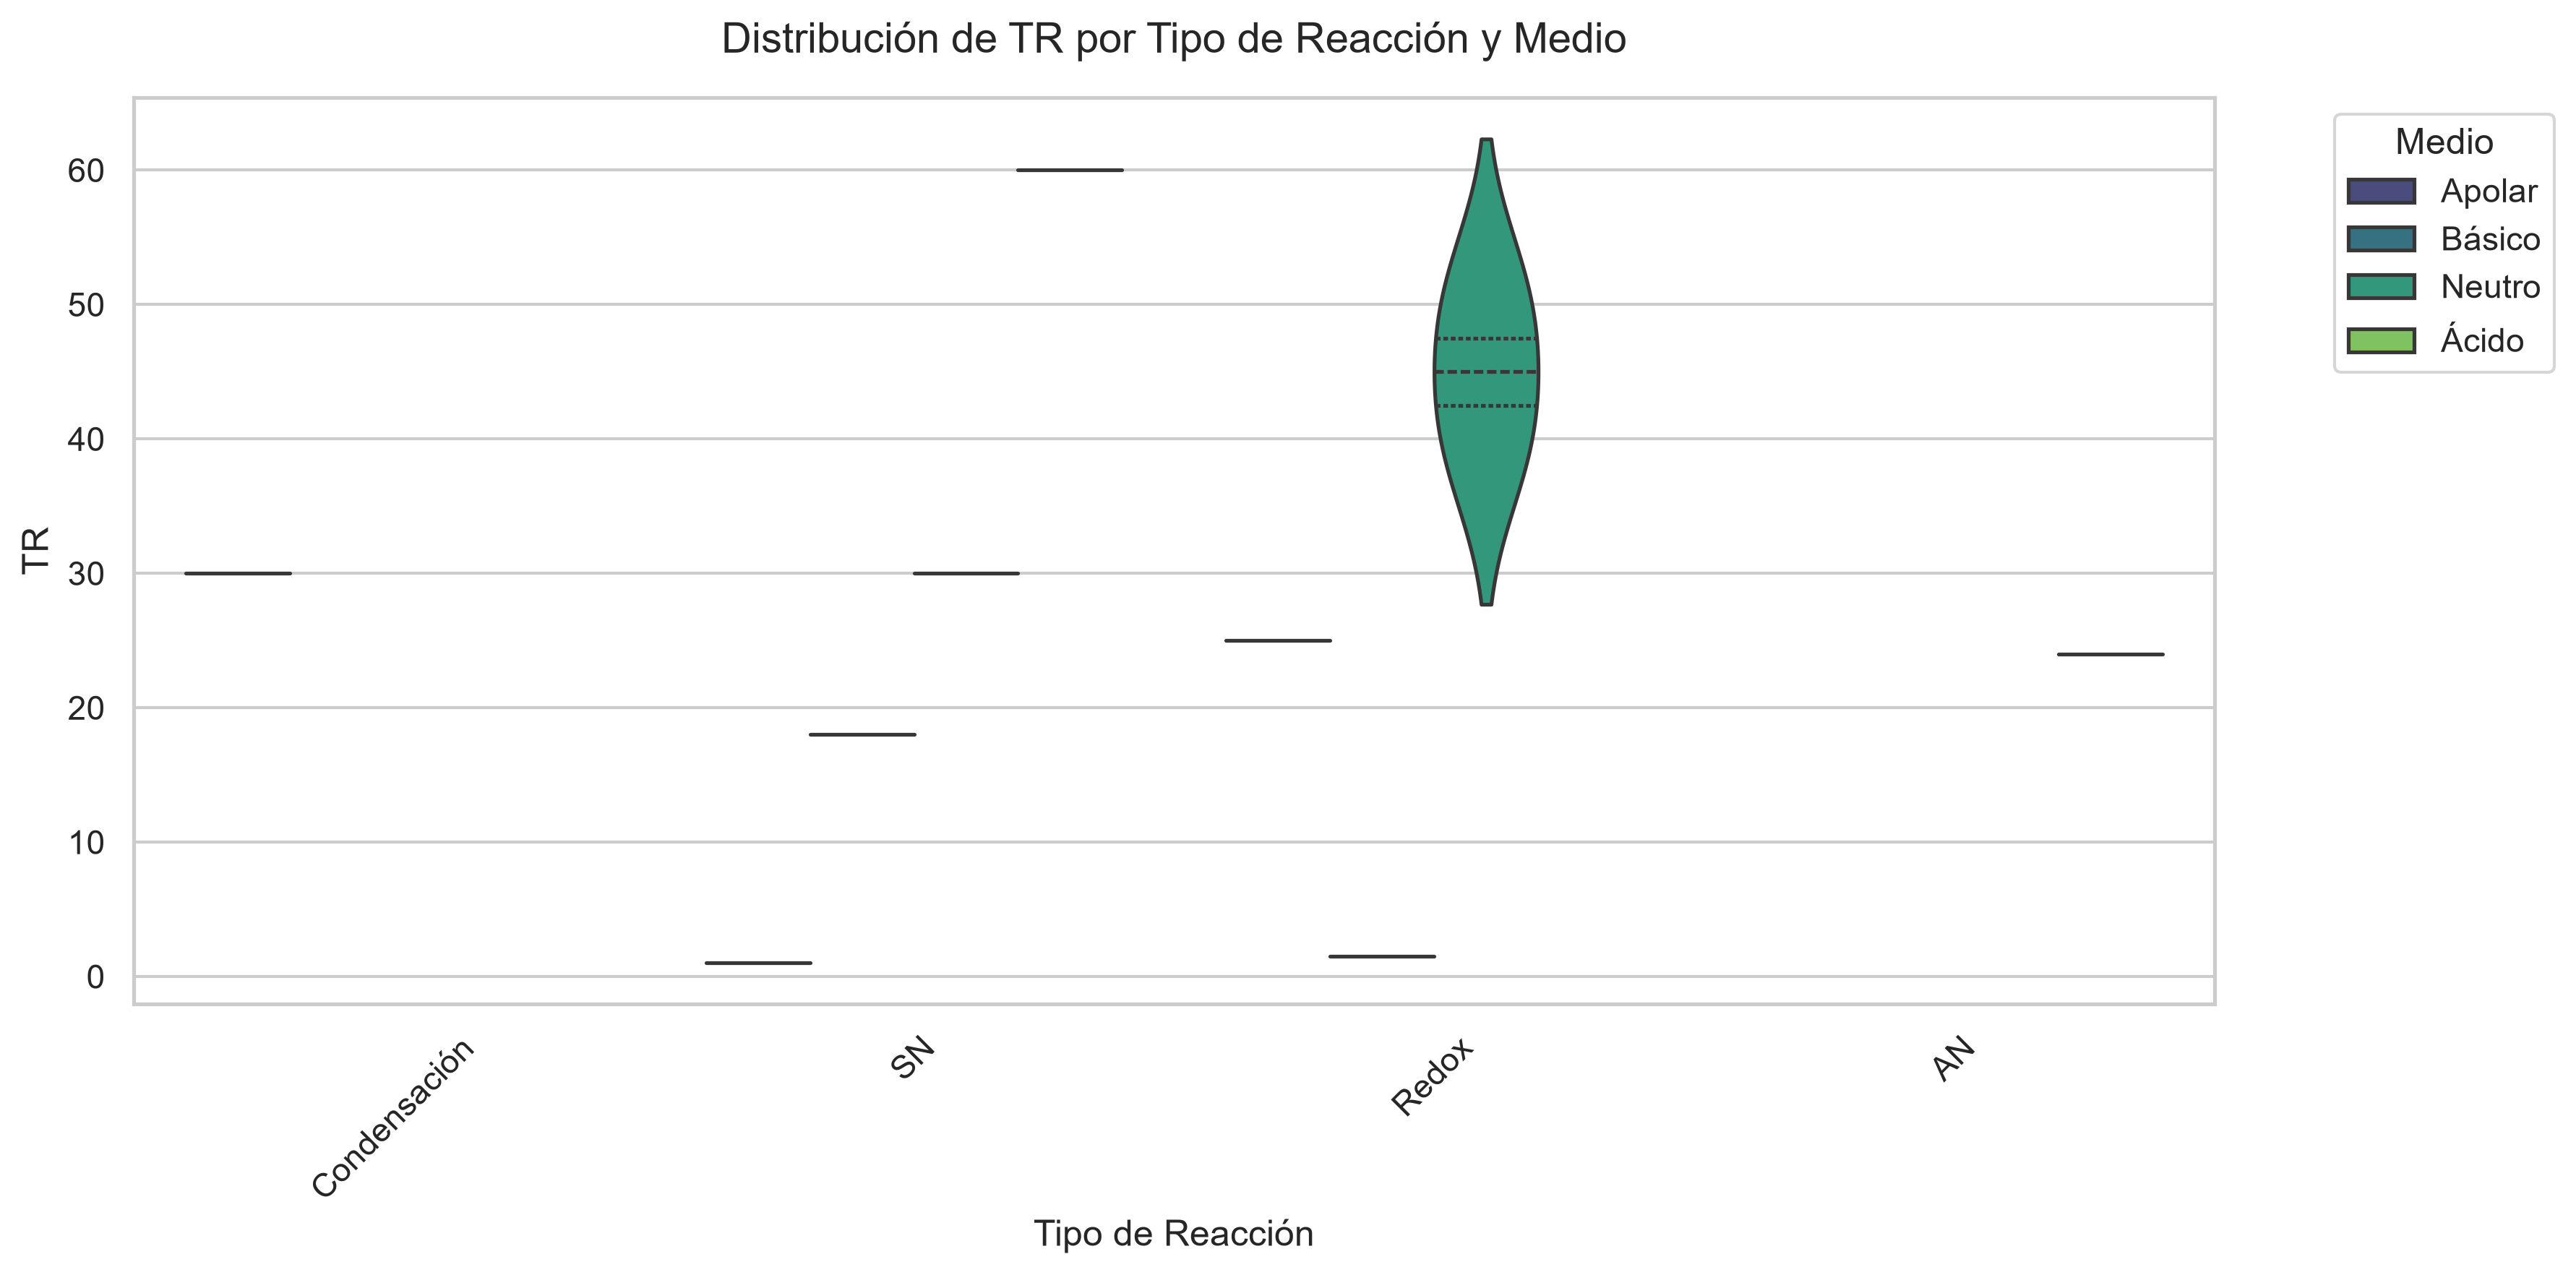
\includegraphics[width=\columnwidth]{07_violin_TR_tipo_medio.png}
	\caption{Distribución (violín) de TR por tipo de reacción y medio.}
	\label{fig:violin}
\end{figure}

\begin{figure}[htbp]
	\centering
	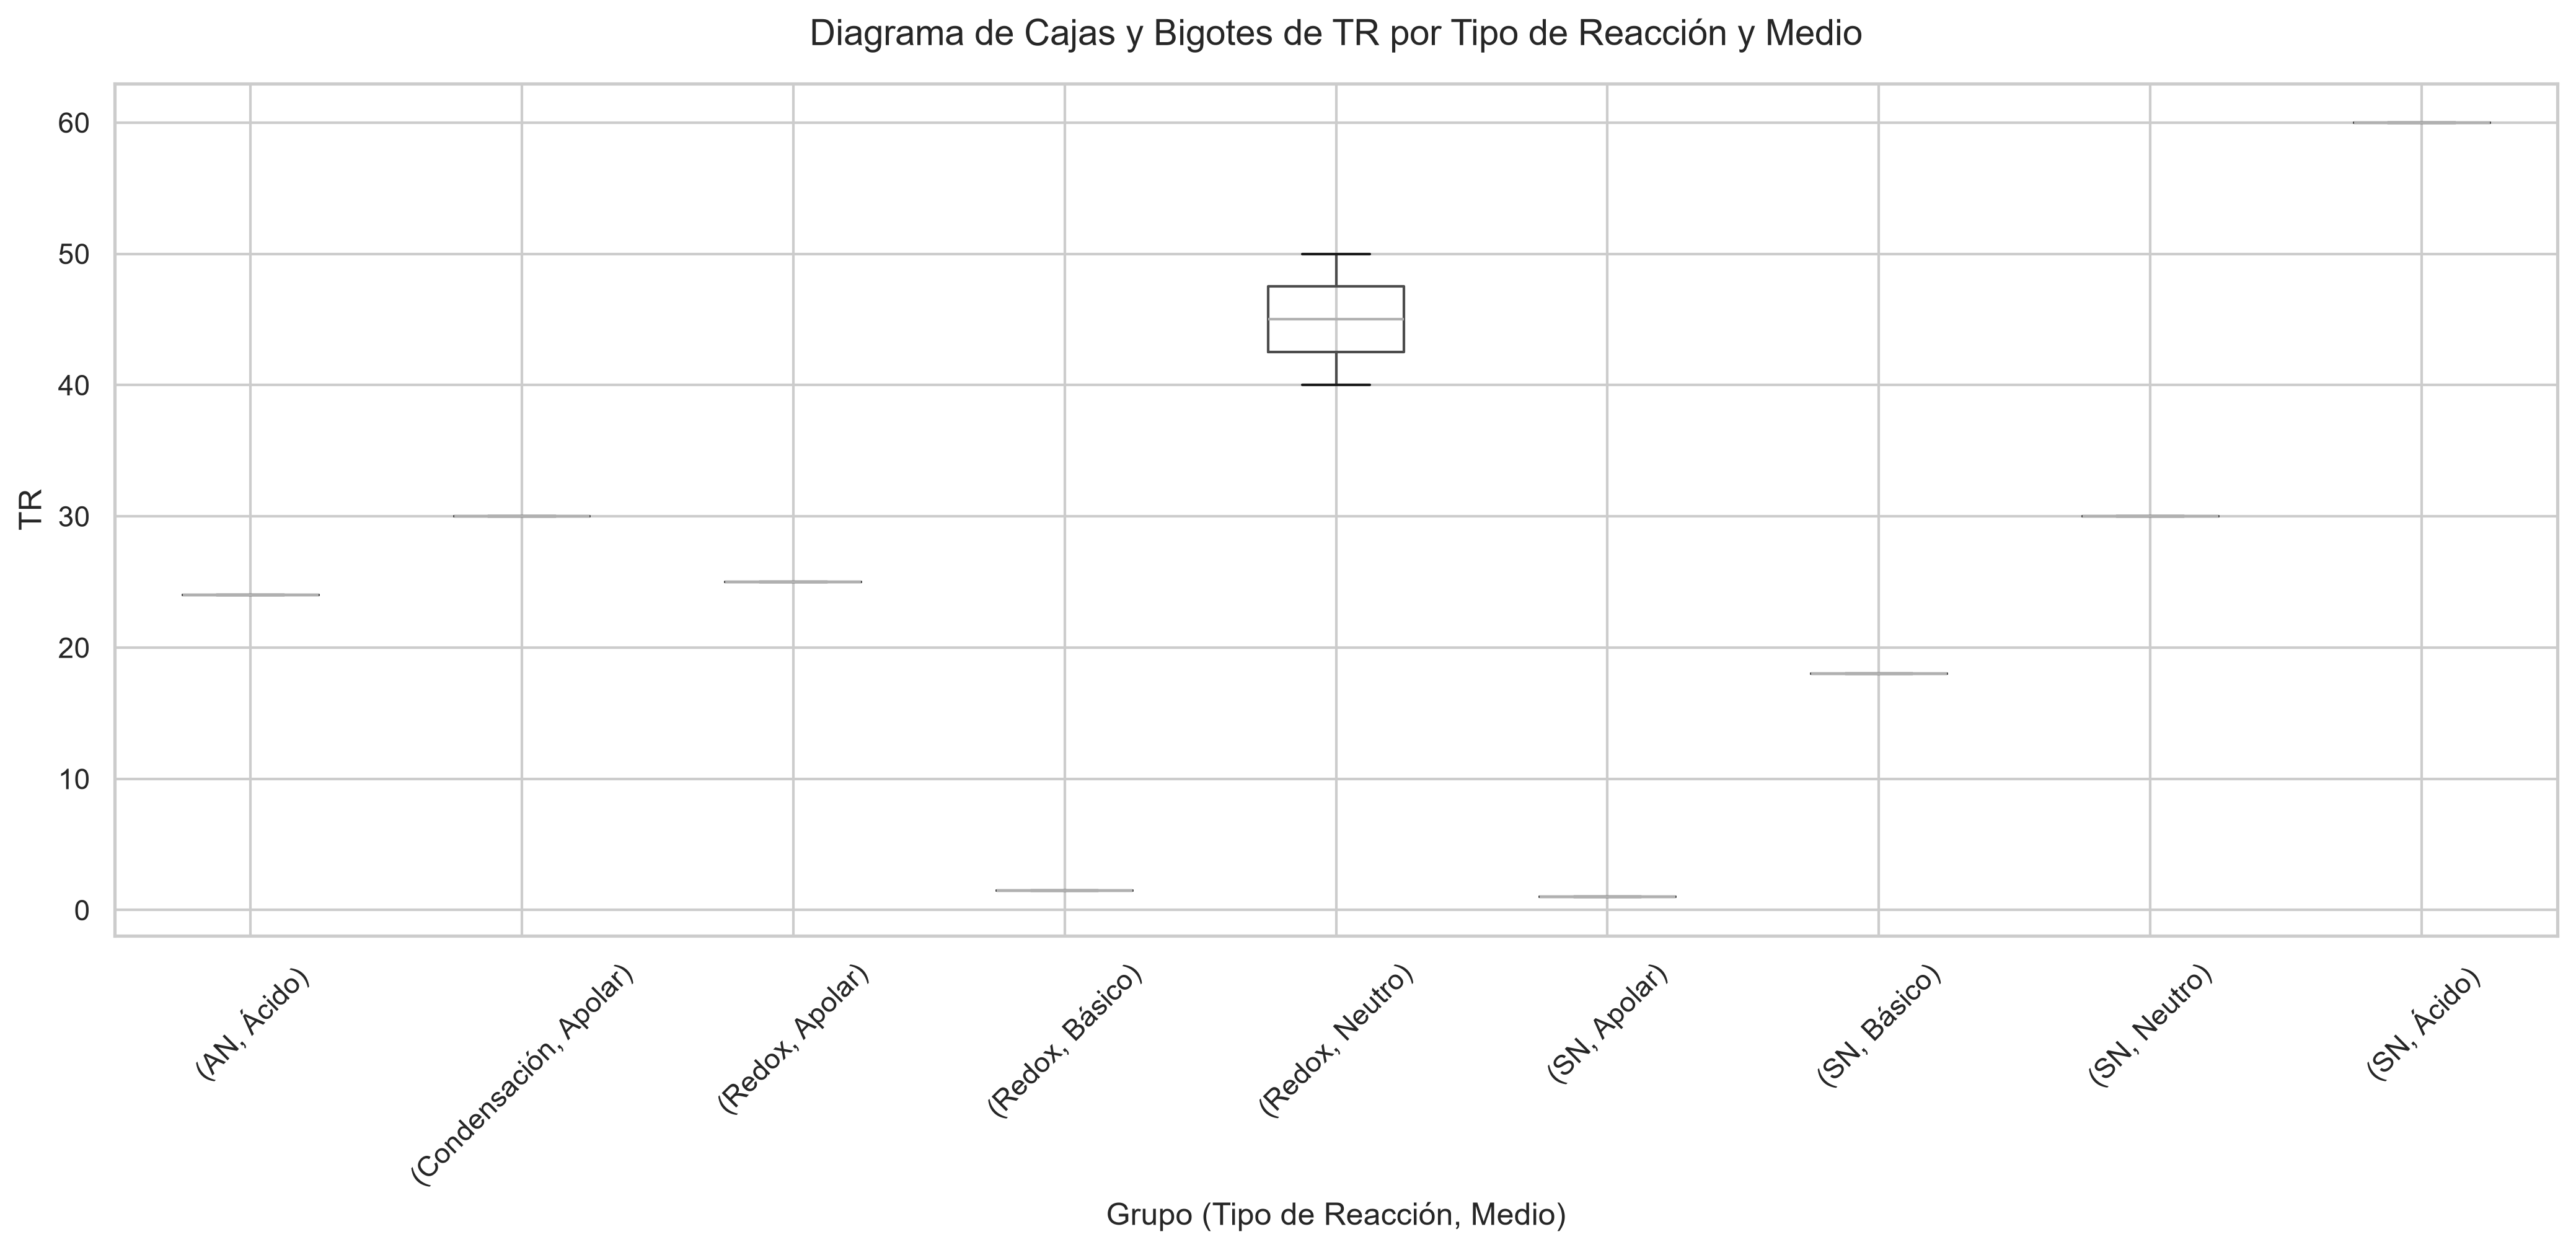
\includegraphics[width=\columnwidth]{08_boxplot_TR_tipo_medio.png}
	\caption{Diagrama de cajas y bigotes de TR por tipo de reacción y medio.}
	\label{fig:boxplot}
\end{figure}

\begin{figure}[htbp]
	\centering
	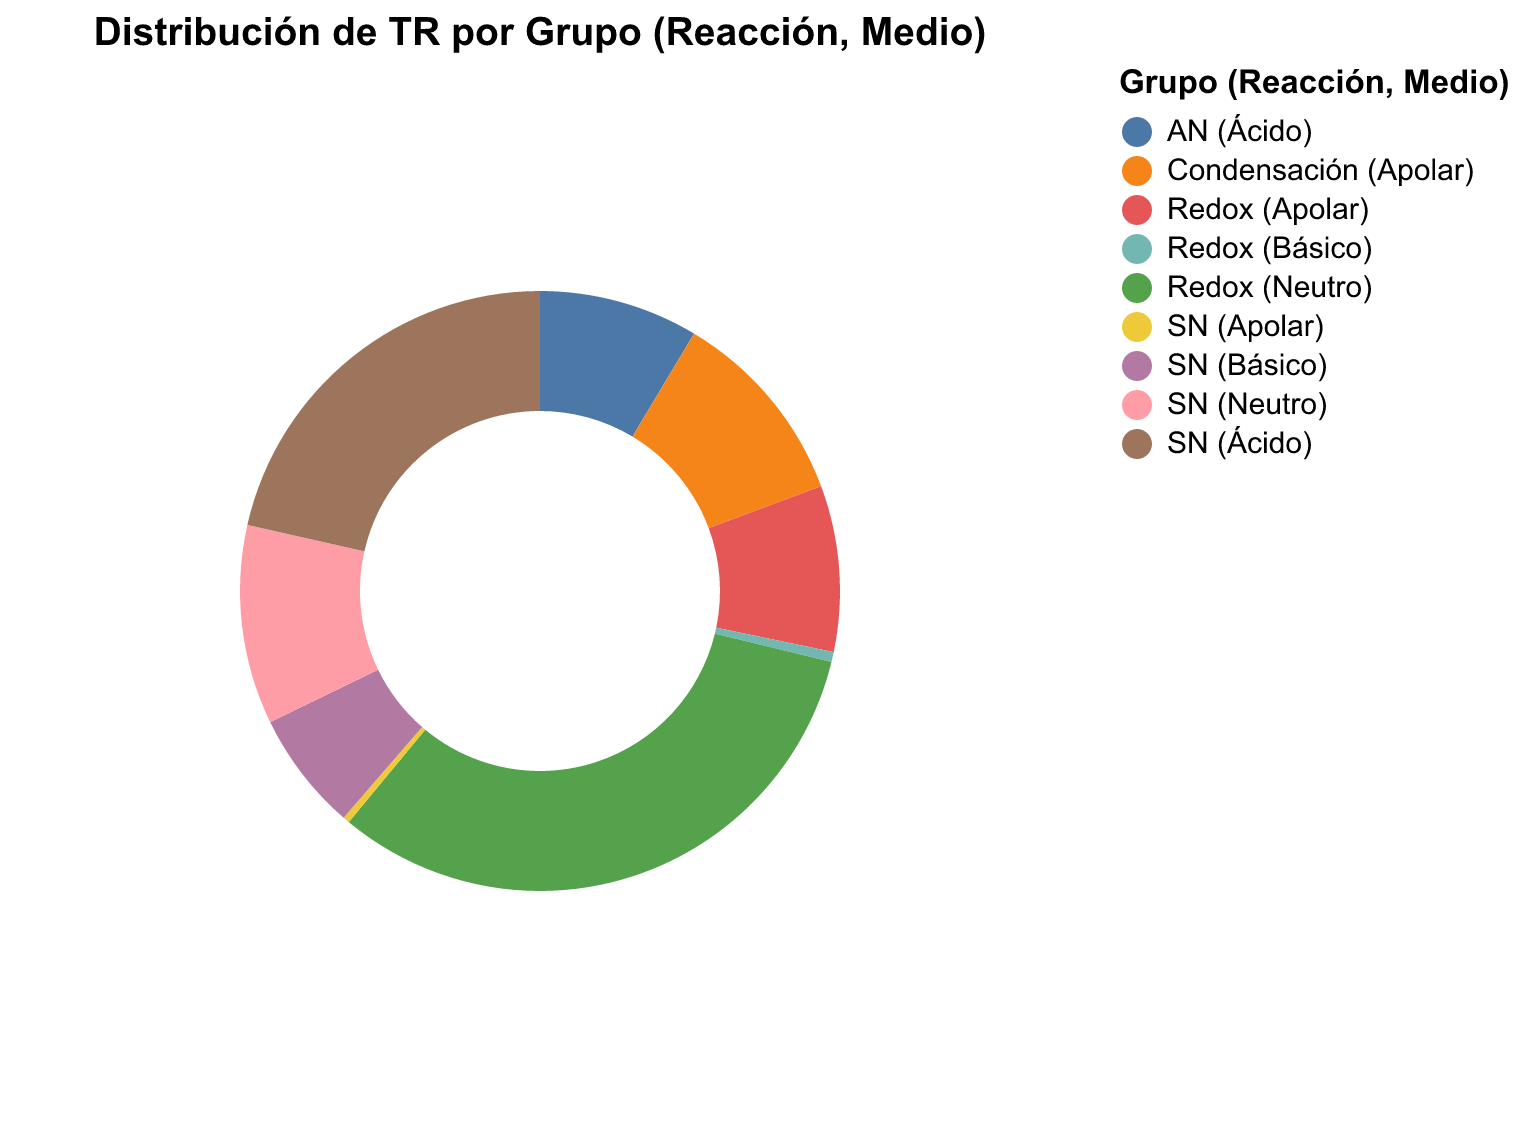
\includegraphics[width=0.9\columnwidth]{10_dona_TR_grupo.png}
	\caption{Participación de TR por grupo (tipo de reacción, medio).}
	\label{fig:dona}
\end{figure}

\section{Conclusiones y Perspectiva}
\fontsize{12}{14}\selectfont
% TODO (Valentina): 3--5 conclusiones que respondan al objetivo de la introducción,
% cada una sustentada en una figura o en la Tabla~\ref{tab:propiedades}.
\textit{[Redacción pendiente.]}

%  Contenido: Metodología, Análisis Gráfico (Colab/Conda) y Conclusiones
%
%  Reglas para editar sin romper la compilación:
%   * NO escribir \documentclass, \begin{document} ni \end{document} aquí.
%   * Las figuras están en ../imagenes/ y se llaman sólo por su nombre
%     (main.tex ya define \graphicspath{{imagenes/}}).
%   * Referenciar figuras con Figura~\ref{fig:...}, nunca "la figura de abajo".
% =====================================================================

\section{Metodología}
\fontsize{12}{14}\selectfont
% TODO (Valentina): pegar aquí la redacción de la metodología.

\subsection{Recolección de datos}
\textit{[Redacción pendiente: búsqueda en CAS-SciFinder, compuestos e indicadores asignados, consolidación en Excel con formato Tabla.]}

\subsection{Limpieza y procesamiento en Python}
\textit{[Redacción pendiente: Google Colab con Pandas, NumPy, Matplotlib, Seaborn y Plotly; filtrado de los compuestos de interés, conversión de comas decimales, tratamiento de valores nulos y atípicos.]}

\subsection{Análisis estadístico}
\textit{[Redacción pendiente: correlación de Spearman (no paramétrica, robusta a valores atípicos y relaciones monótonas no lineales), regresiones lineales con intervalo de confianza del 95\,\% y distribuciones por tipo de reacción y medio.]}

\section{Resultados y Discusión}
\fontsize{12}{14}\selectfont

\subsection{Correlación entre propiedades}
% TODO (Valentina): interpretar los coeficientes más fuertes (positivos y negativos).
La Figura~\ref{fig:heatmap} presenta la matriz de correlación de Spearman entre
las propiedades fisicoquímicas, y la Figura~\ref{fig:clustermap} agrupa
jerárquicamente las variables con comportamiento similar.
\textit{[Interpretación pendiente.]}

\begin{figure}[htbp]
	\centering
	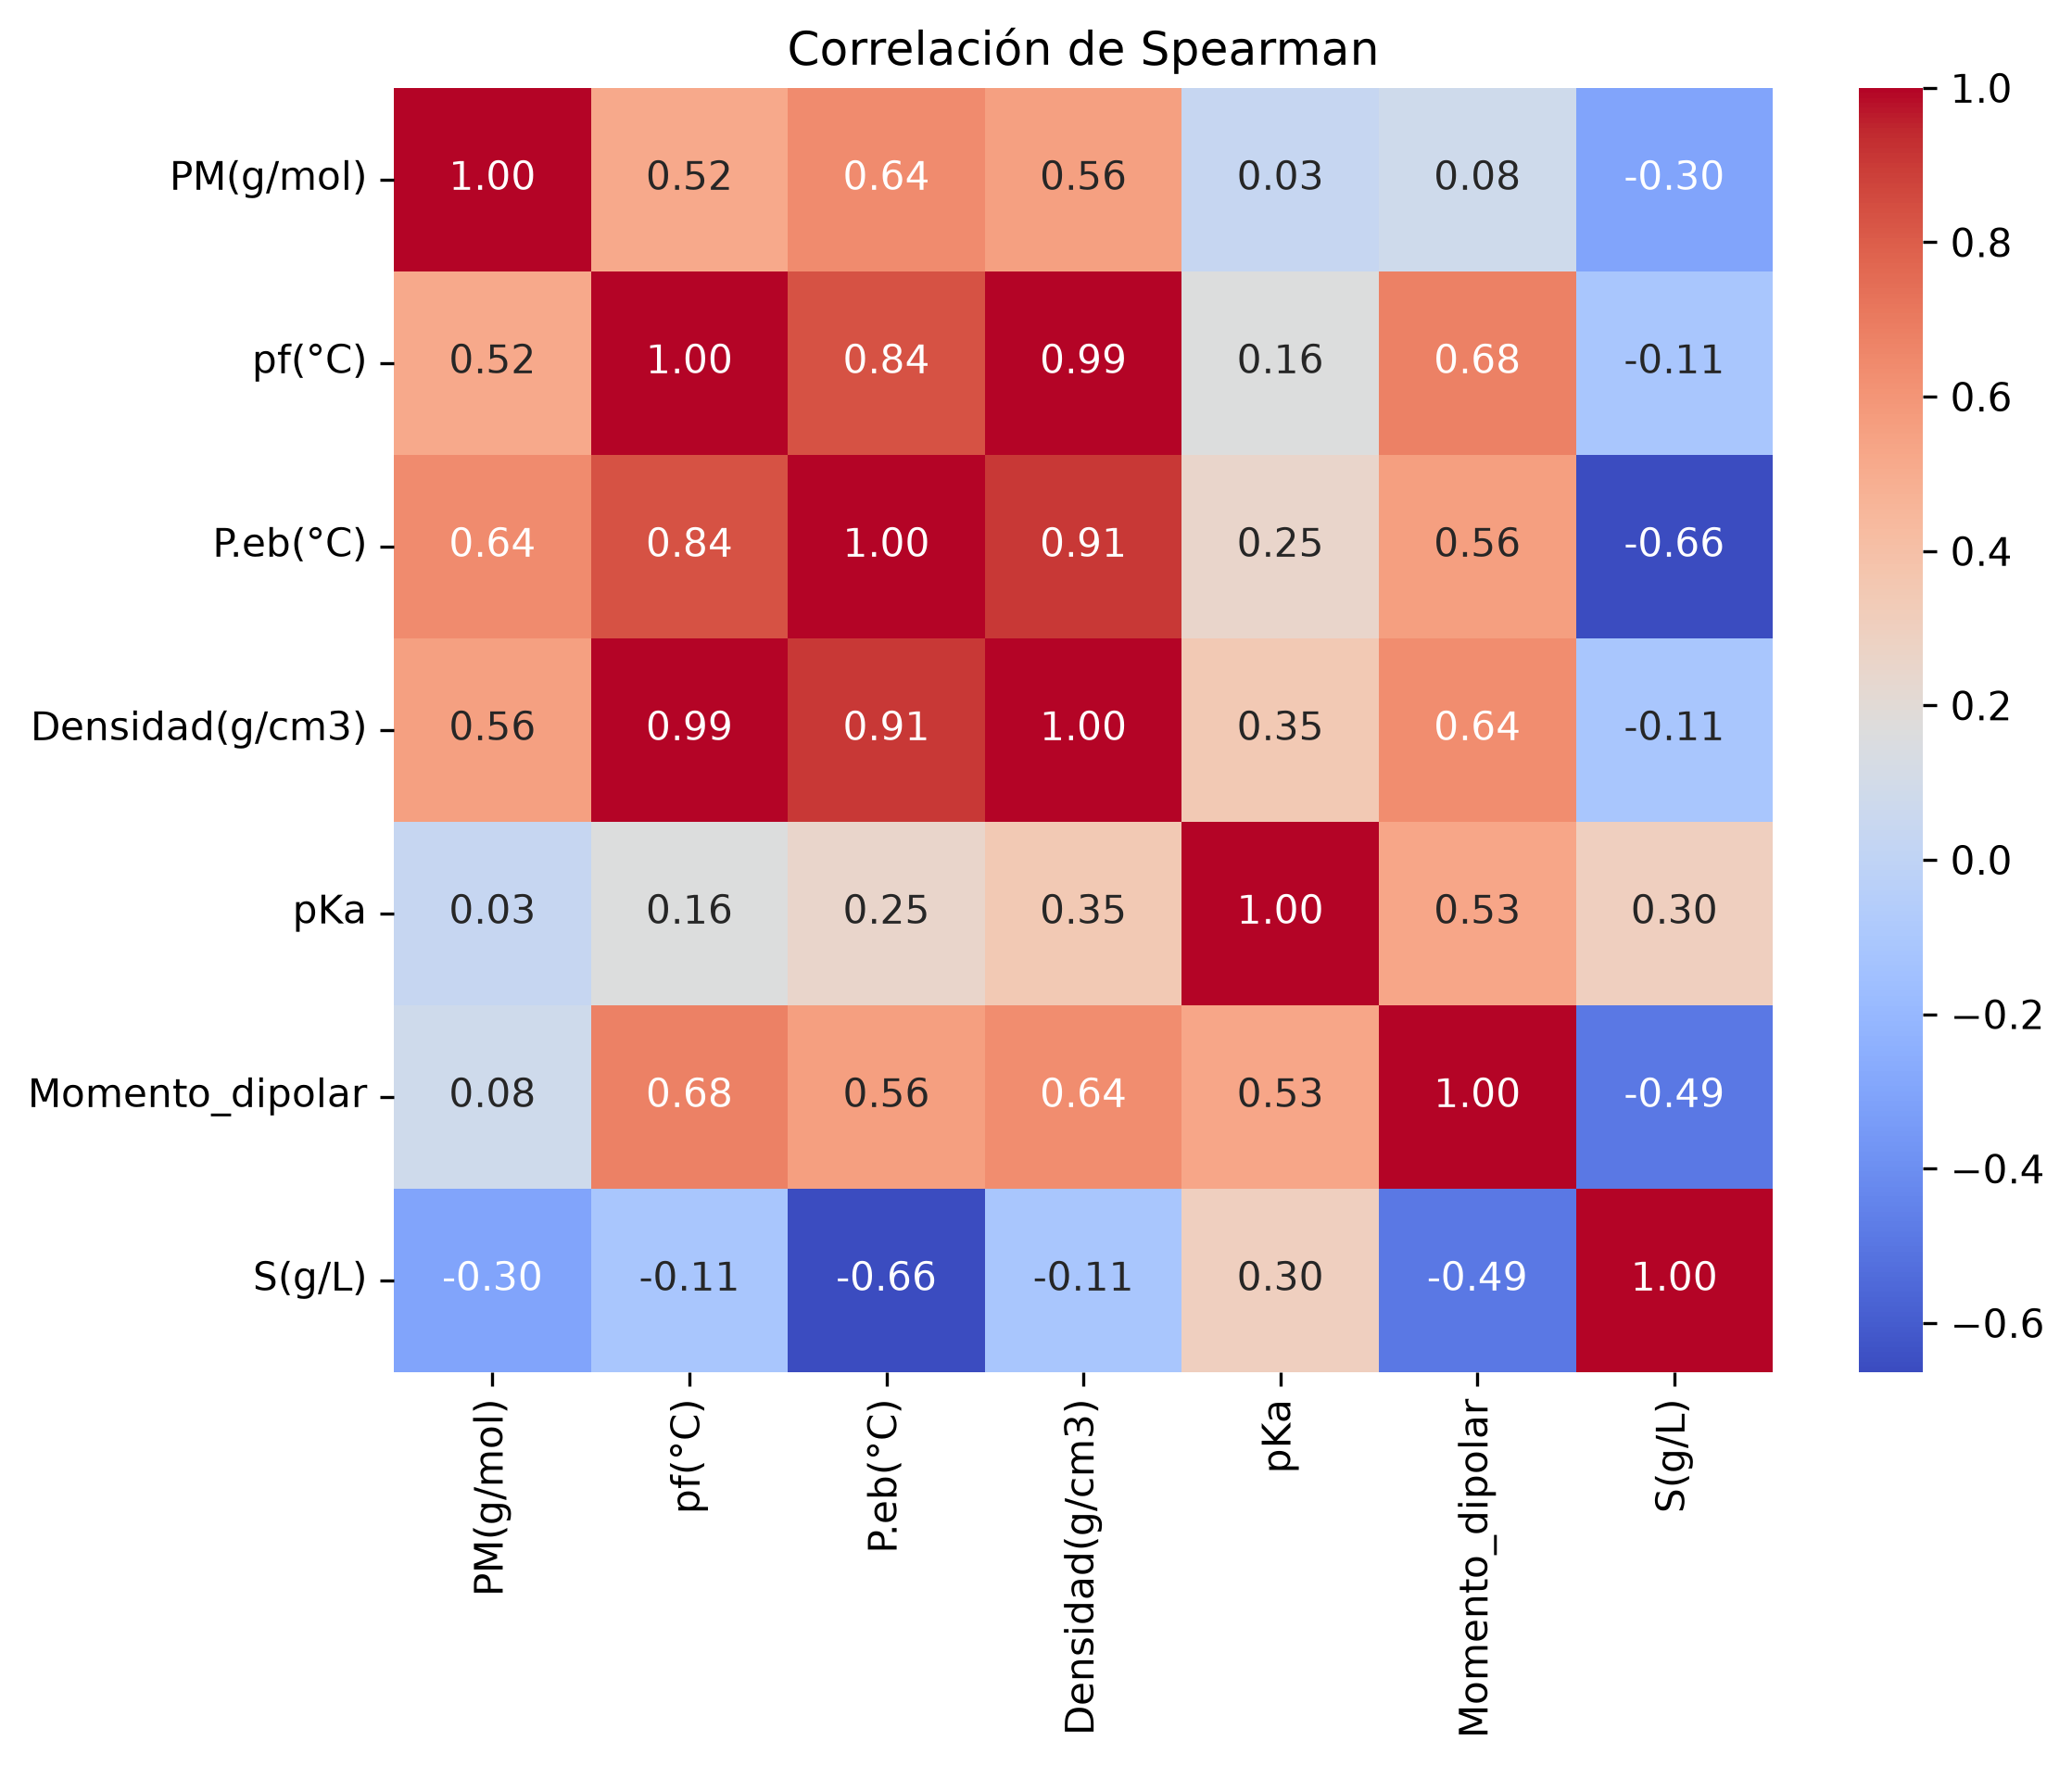
\includegraphics[width=\columnwidth]{01_heatmap_spearman.png}
	\caption{Matriz de correlación de Spearman entre las propiedades fisicoquímicas.}
	\label{fig:heatmap}
\end{figure}

\begin{figure}[htbp]
	\centering
	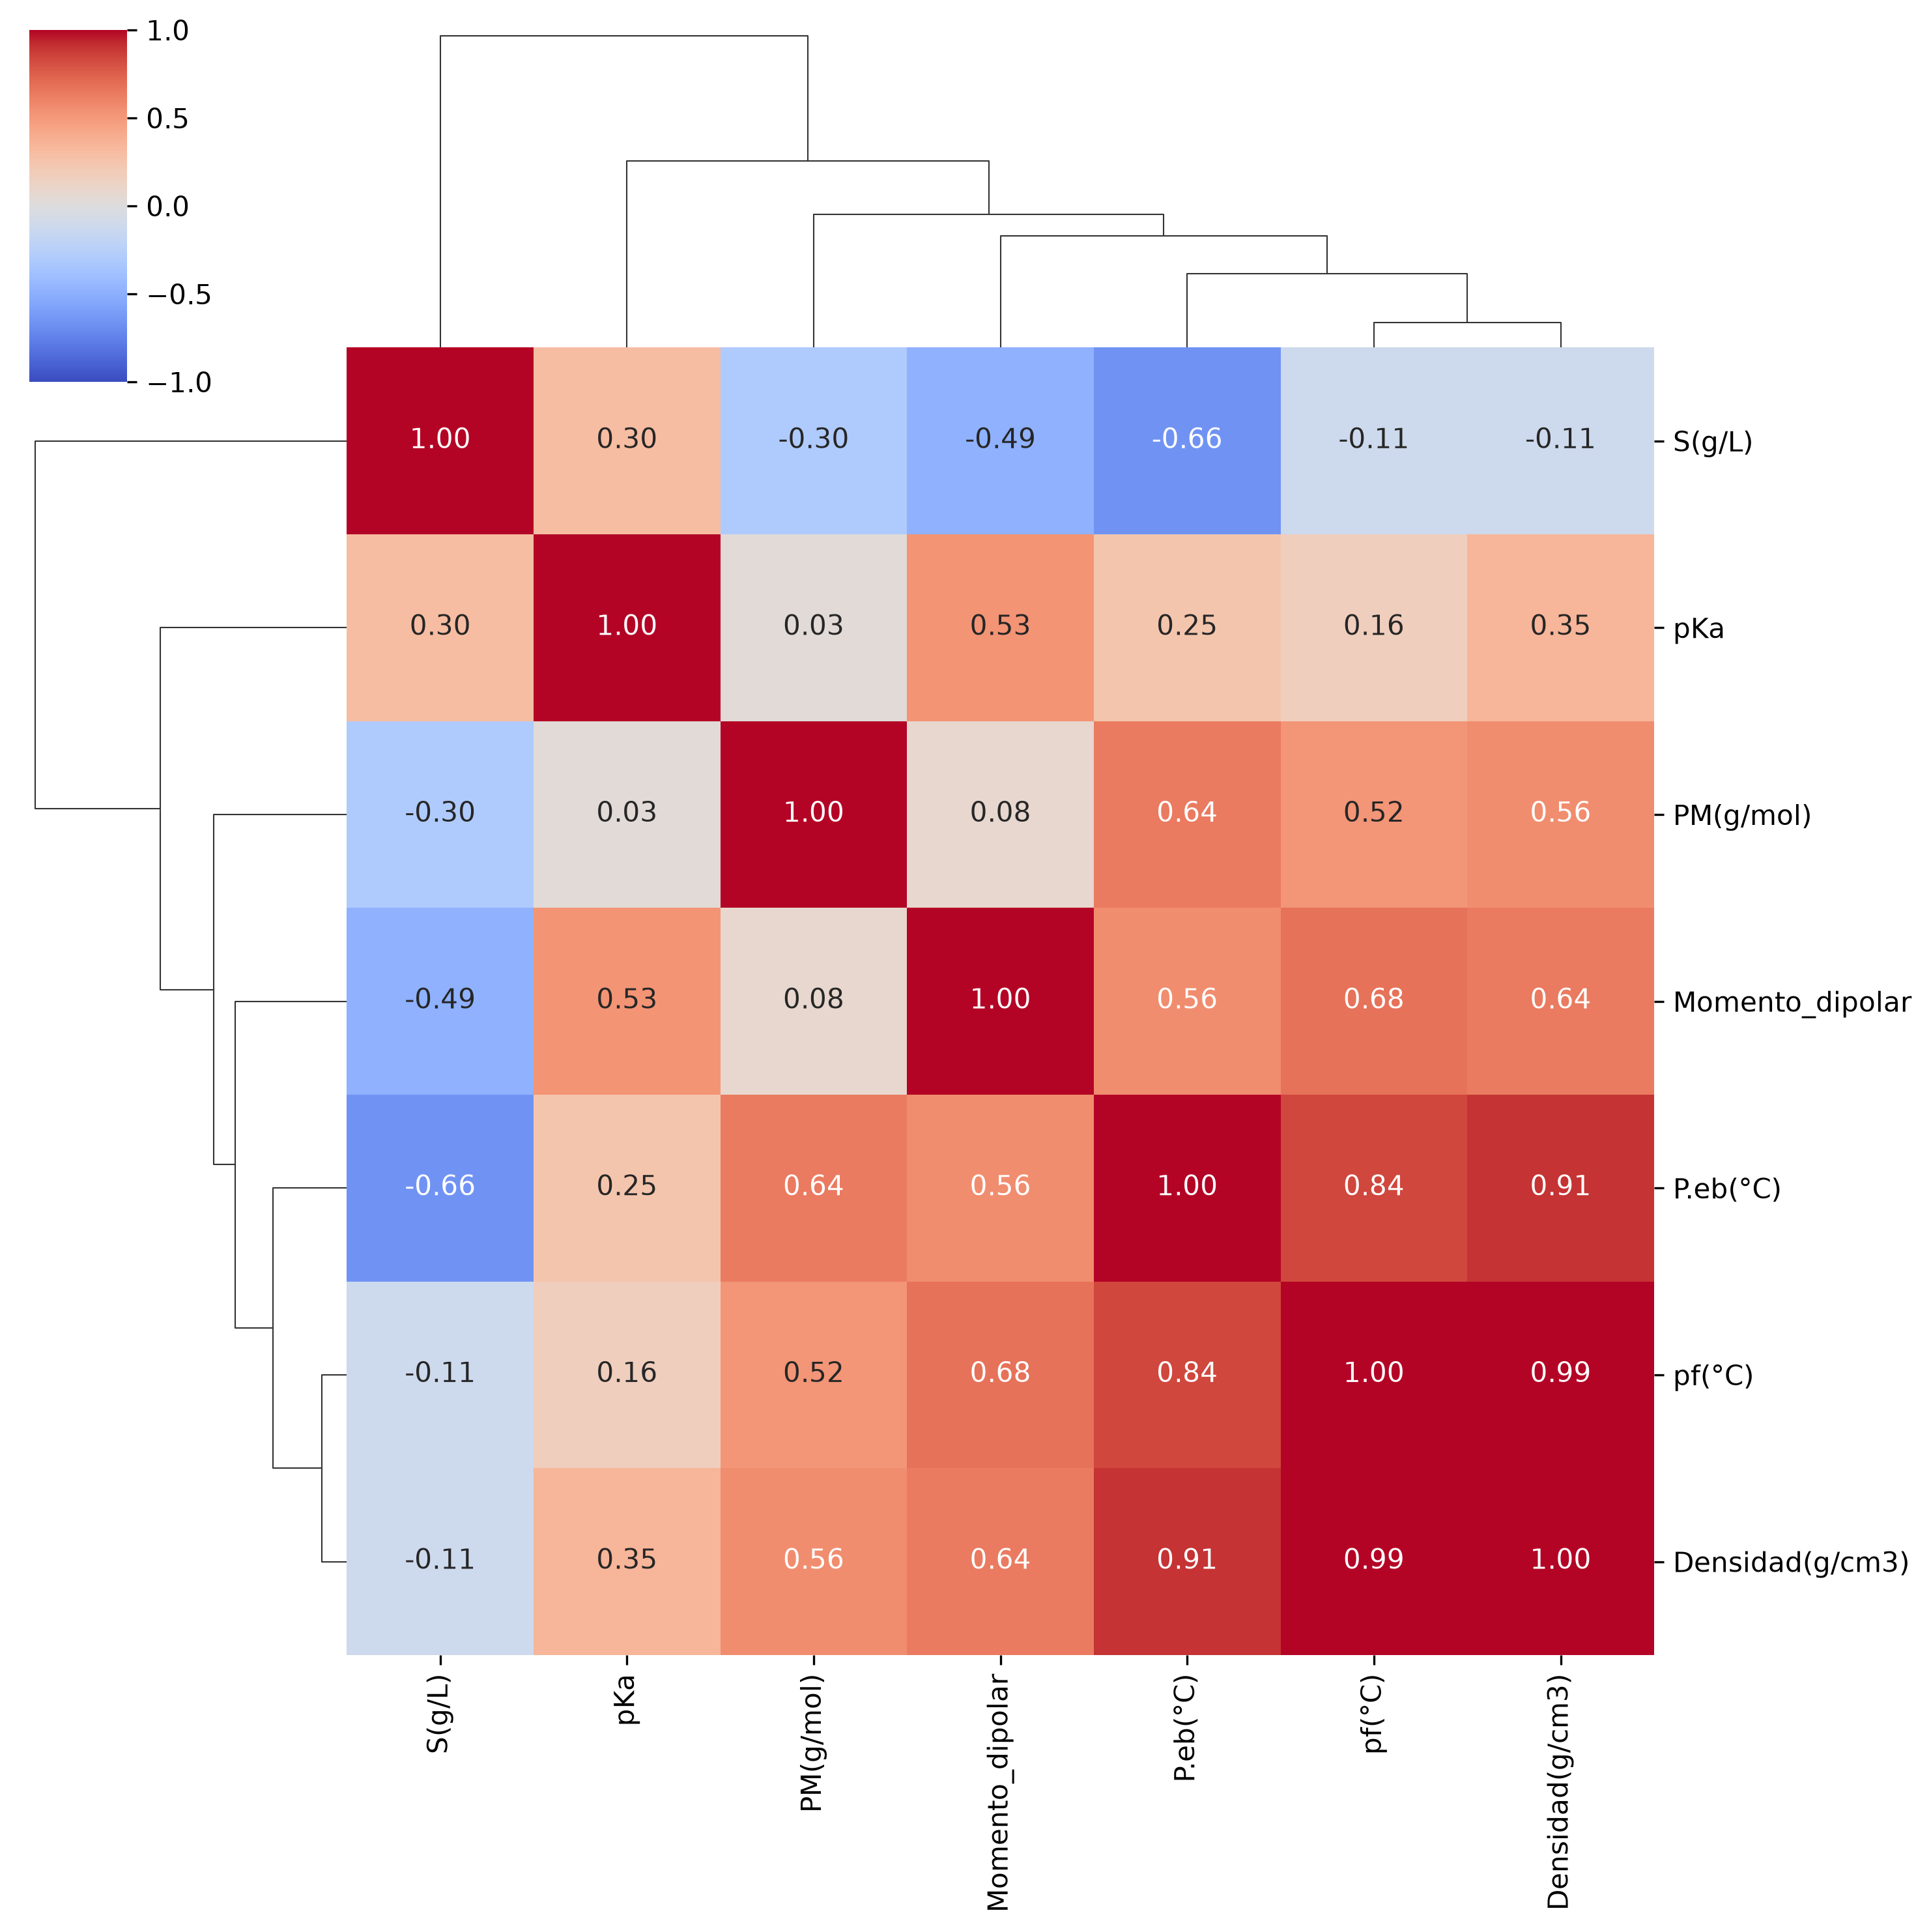
\includegraphics[width=\columnwidth]{02_clustermap_spearman.png}
	\caption{Mapa de agrupamiento jerárquico de la correlación de Spearman.}
	\label{fig:clustermap}
\end{figure}

\subsection{Tendencias entre propiedades}
% TODO (Valentina): discutir cada regresión en términos de fuerzas intermoleculares.
Las Figuras~\ref{fig:pf-dens}--\ref{fig:dip-peb} muestran las regresiones
lineales entre pares de propiedades, con su intervalo de confianza.
\textit{[Interpretación pendiente.]}

\begin{figure}[htbp]
	\centering
	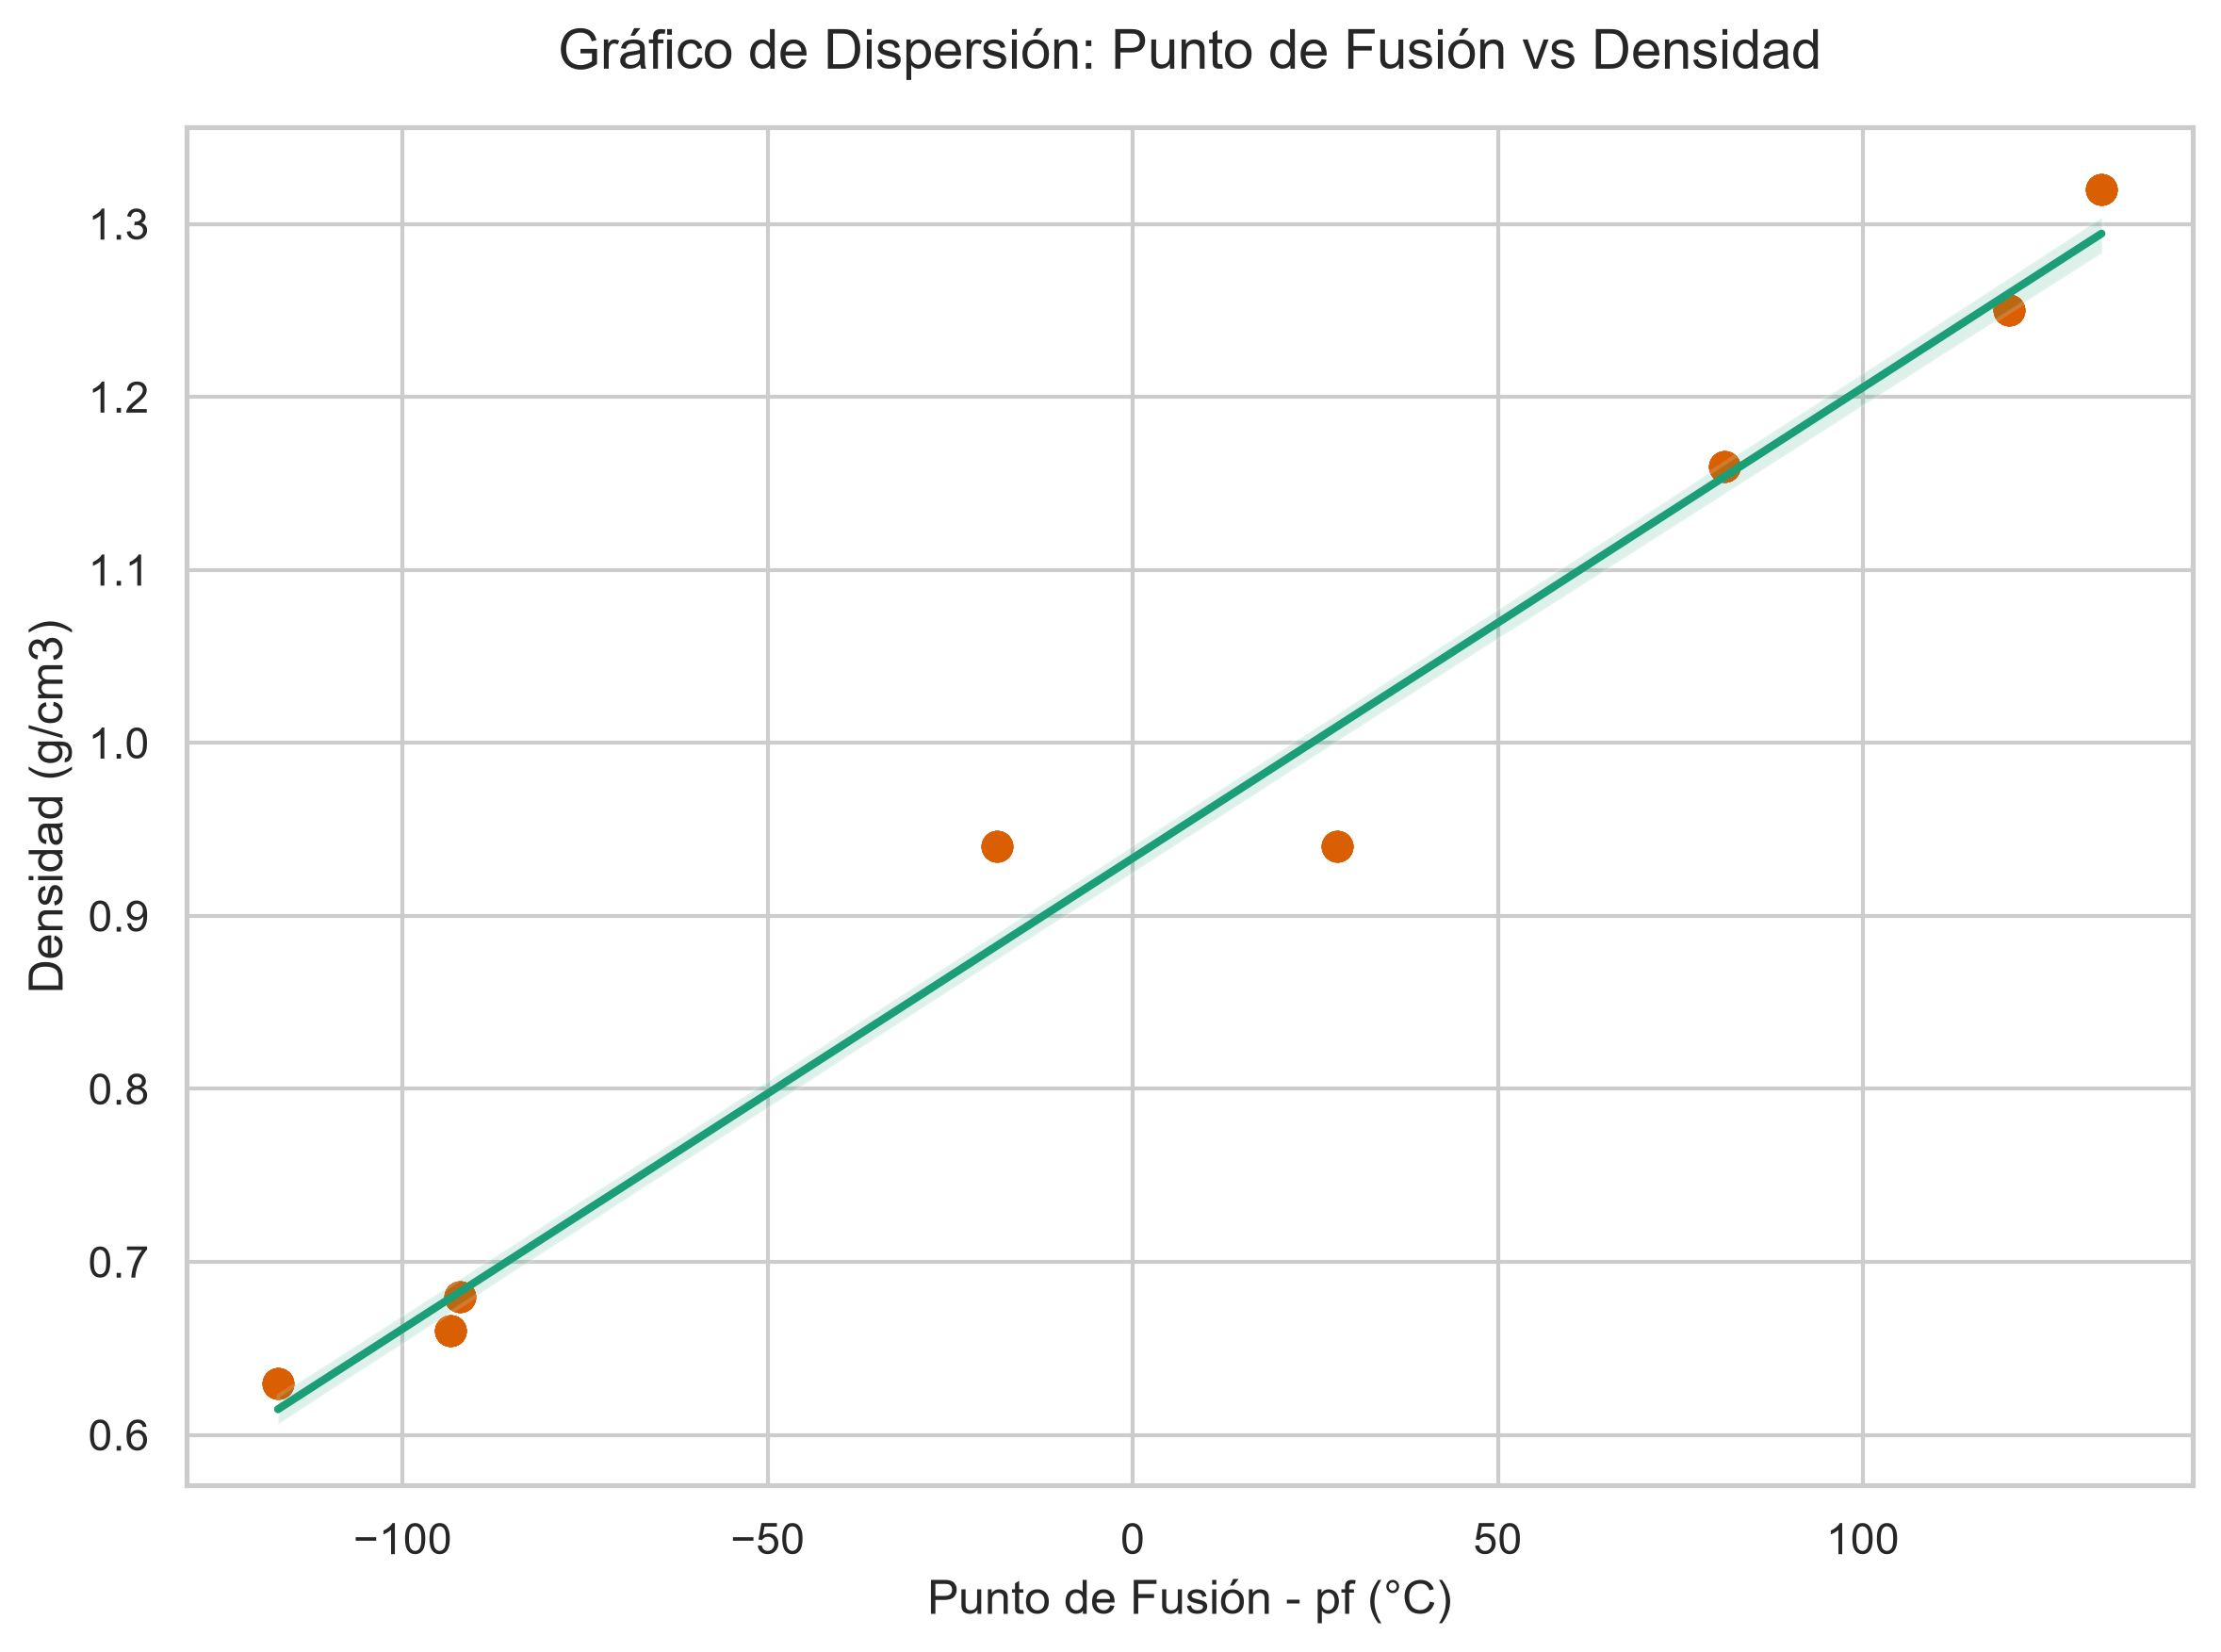
\includegraphics[width=\columnwidth]{03_reg_pf_vs_densidad.png}
	\caption{Punto de fusión frente a densidad.}
	\label{fig:pf-dens}
\end{figure}

\begin{figure}[htbp]
	\centering
	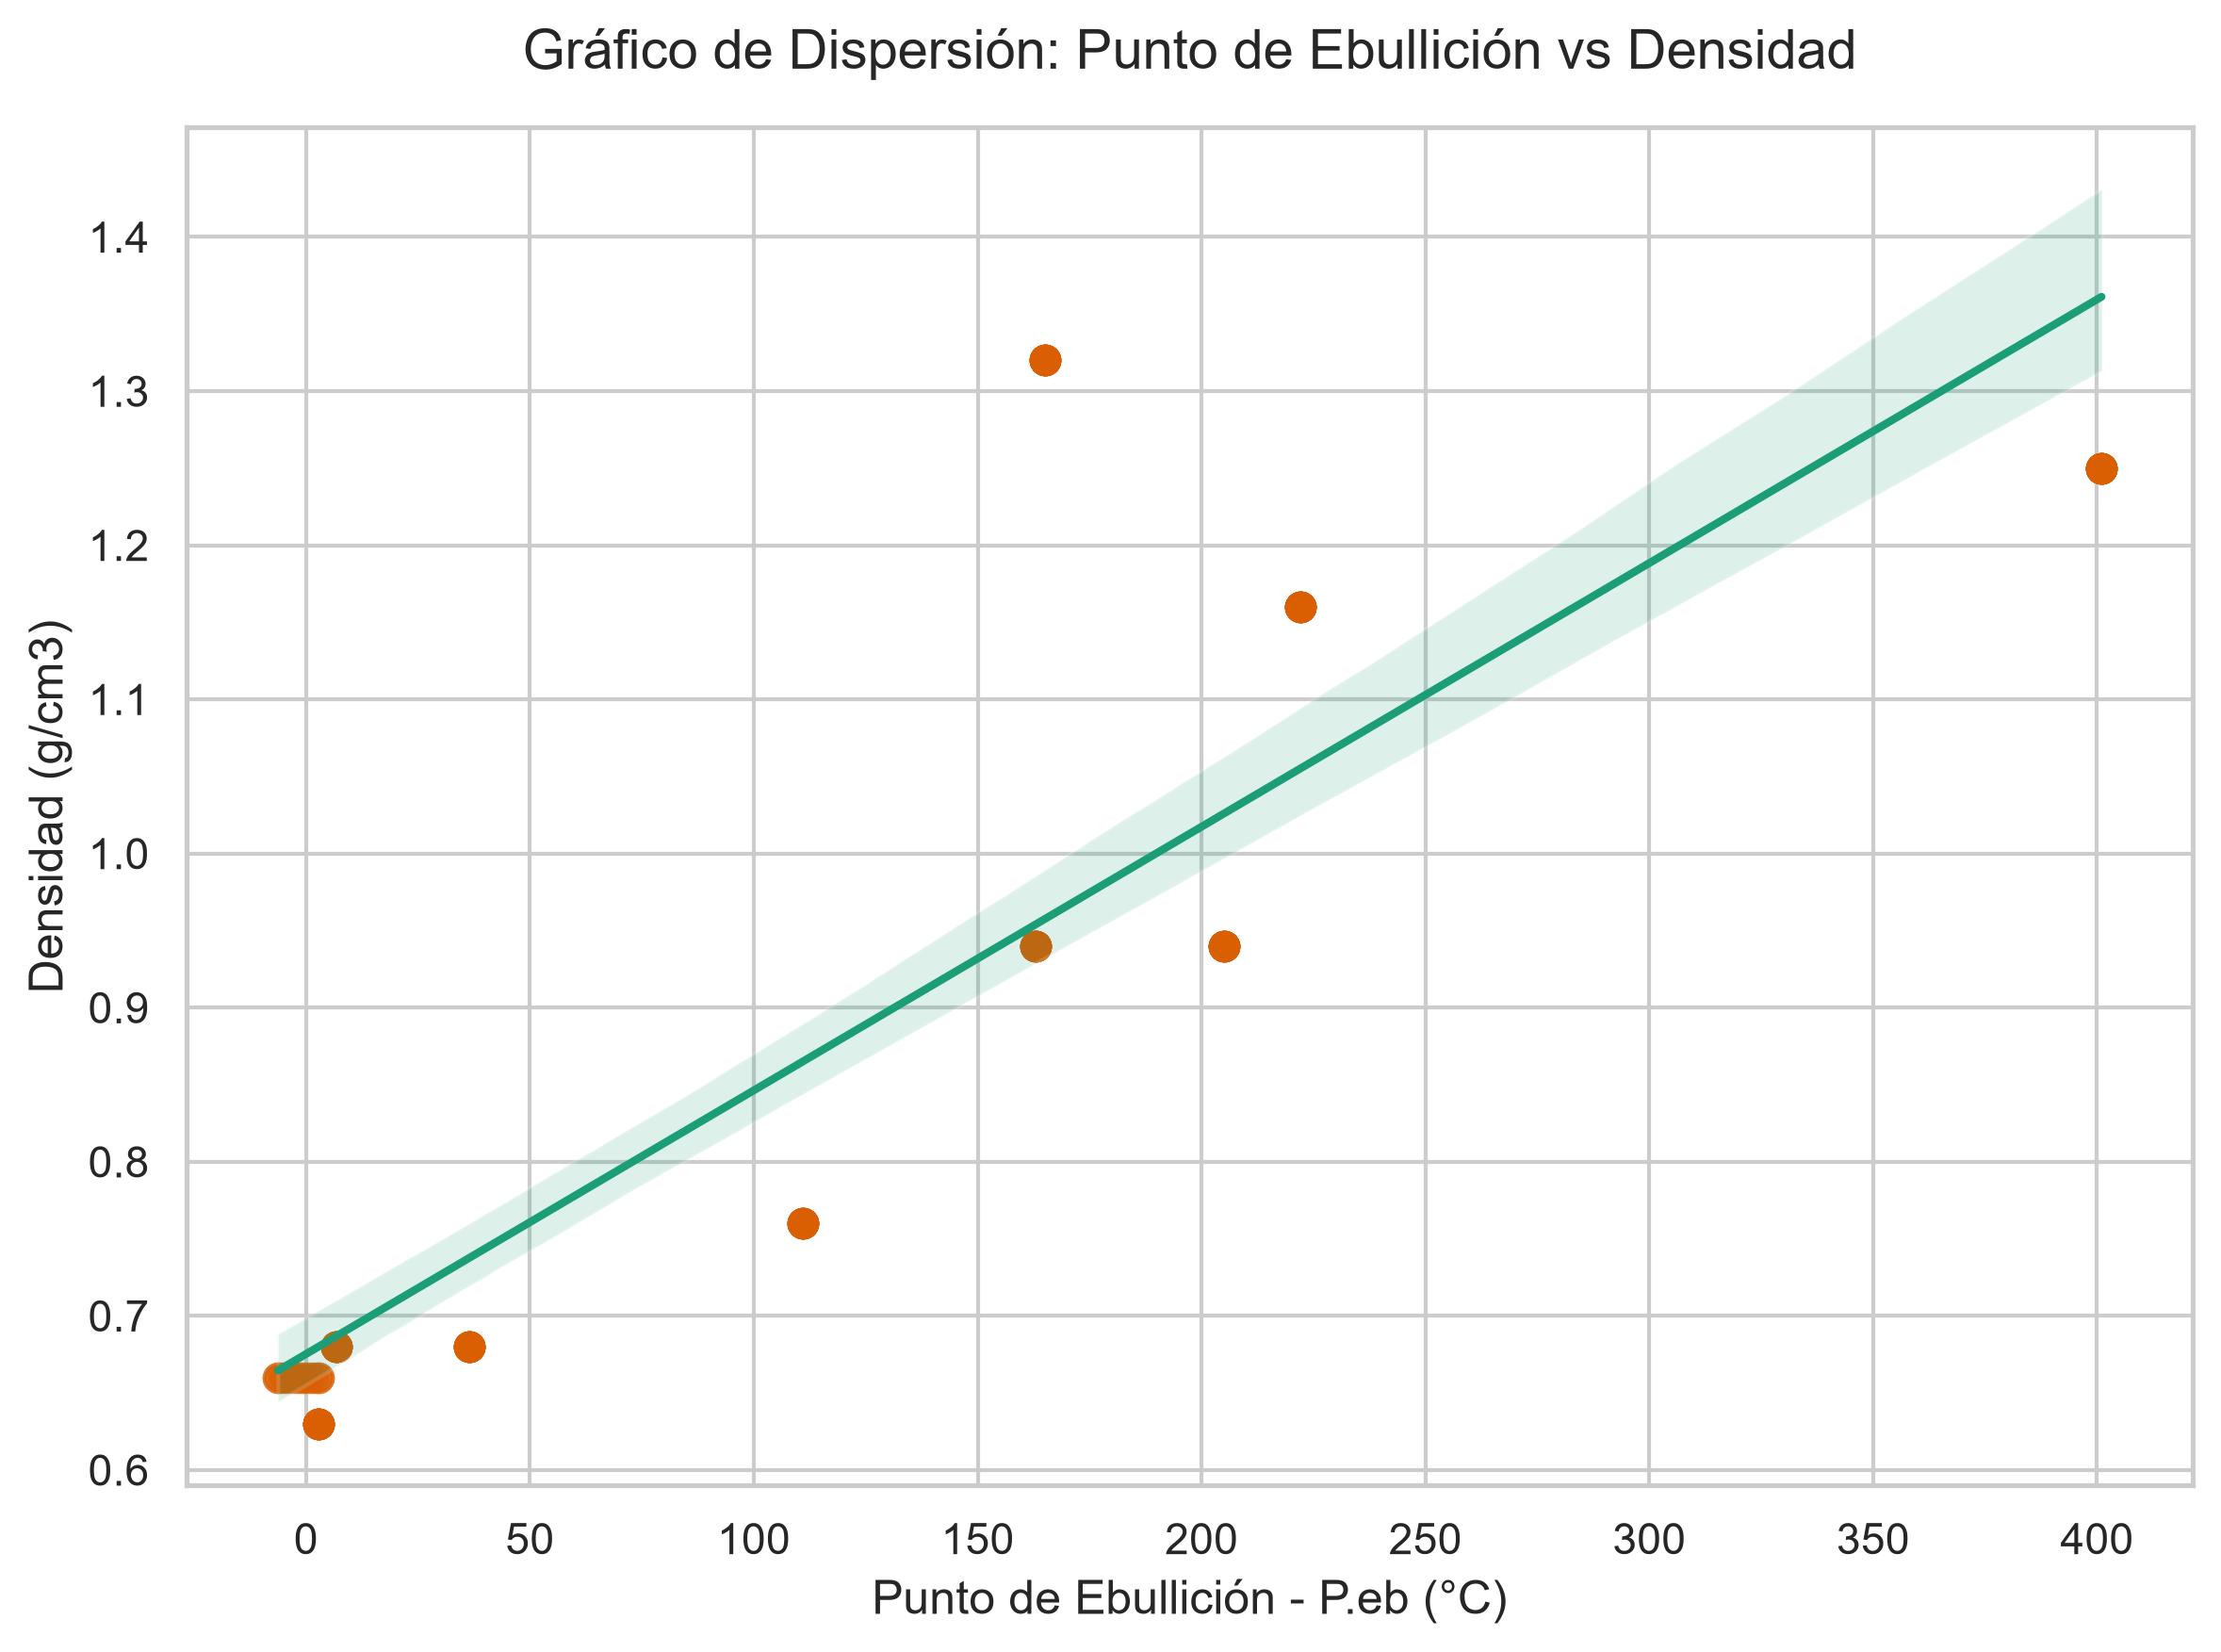
\includegraphics[width=\columnwidth]{04_reg_peb_vs_densidad.png}
	\caption{Punto de ebullición frente a densidad.}
	\label{fig:peb-dens}
\end{figure}

\begin{figure}[htbp]
	\centering
	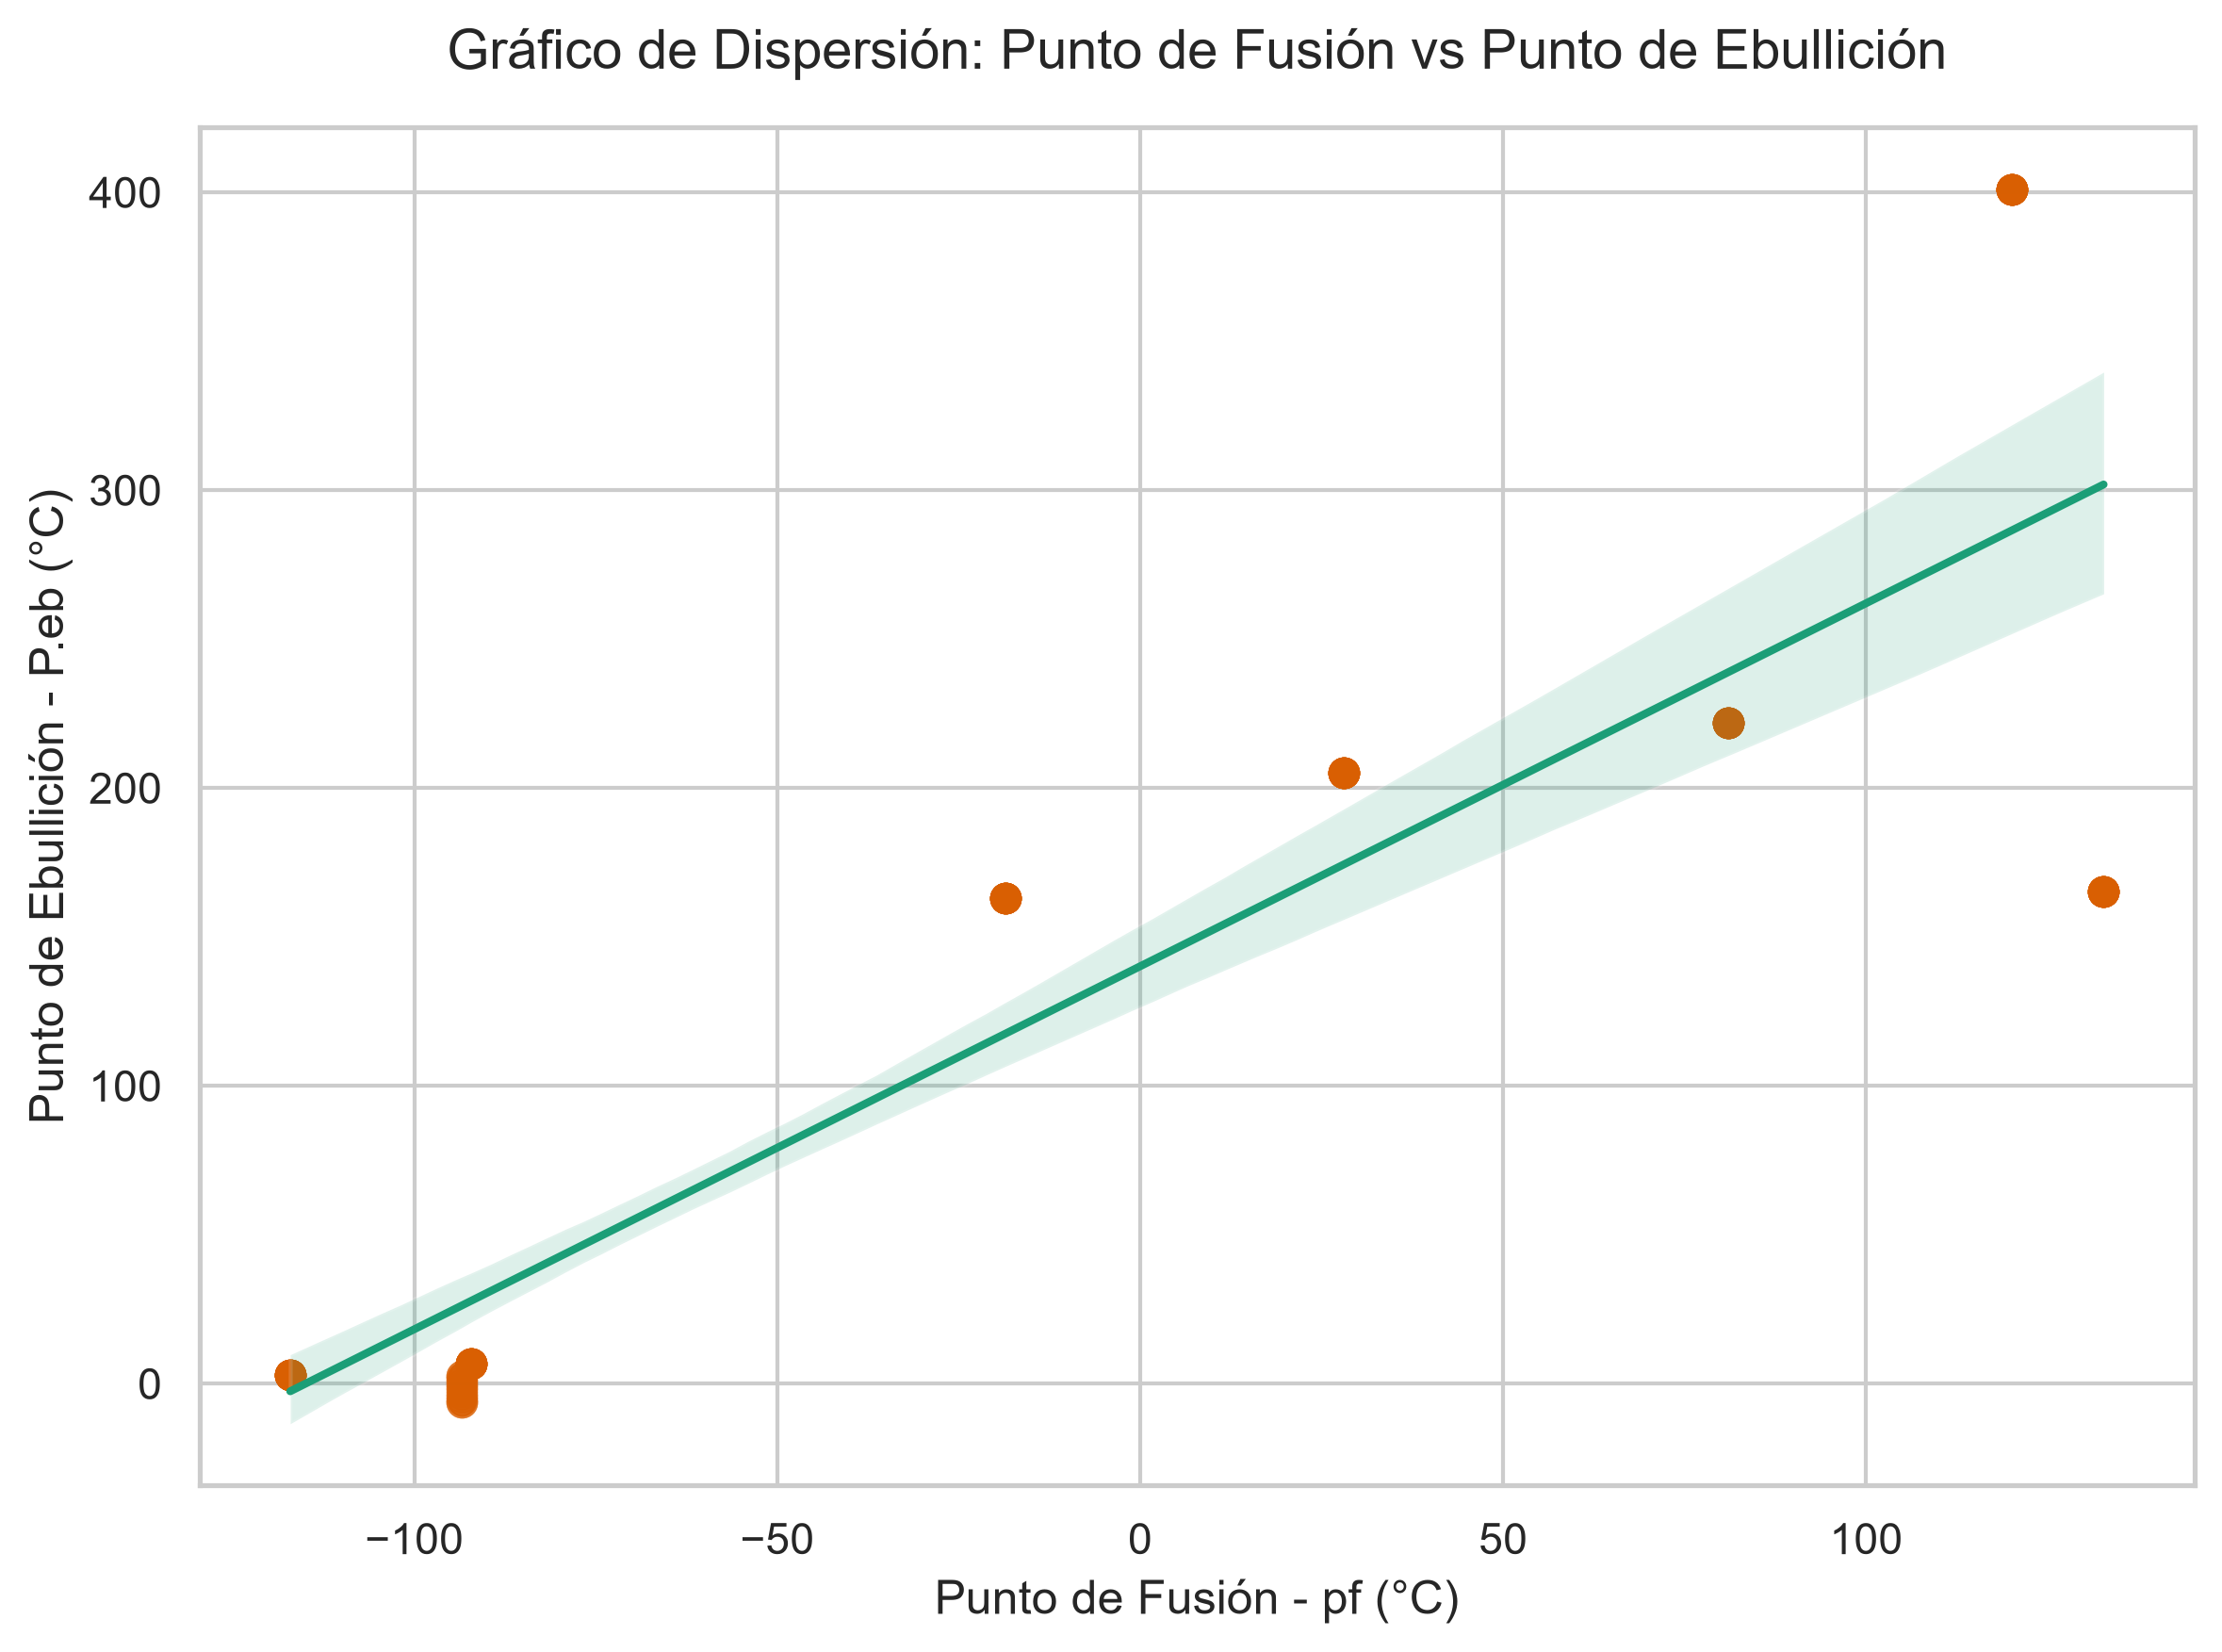
\includegraphics[width=\columnwidth]{05_reg_pf_vs_peb.png}
	\caption{Punto de fusión frente a punto de ebullición.}
	\label{fig:pf-peb}
\end{figure}

\begin{figure}[htbp]
	\centering
	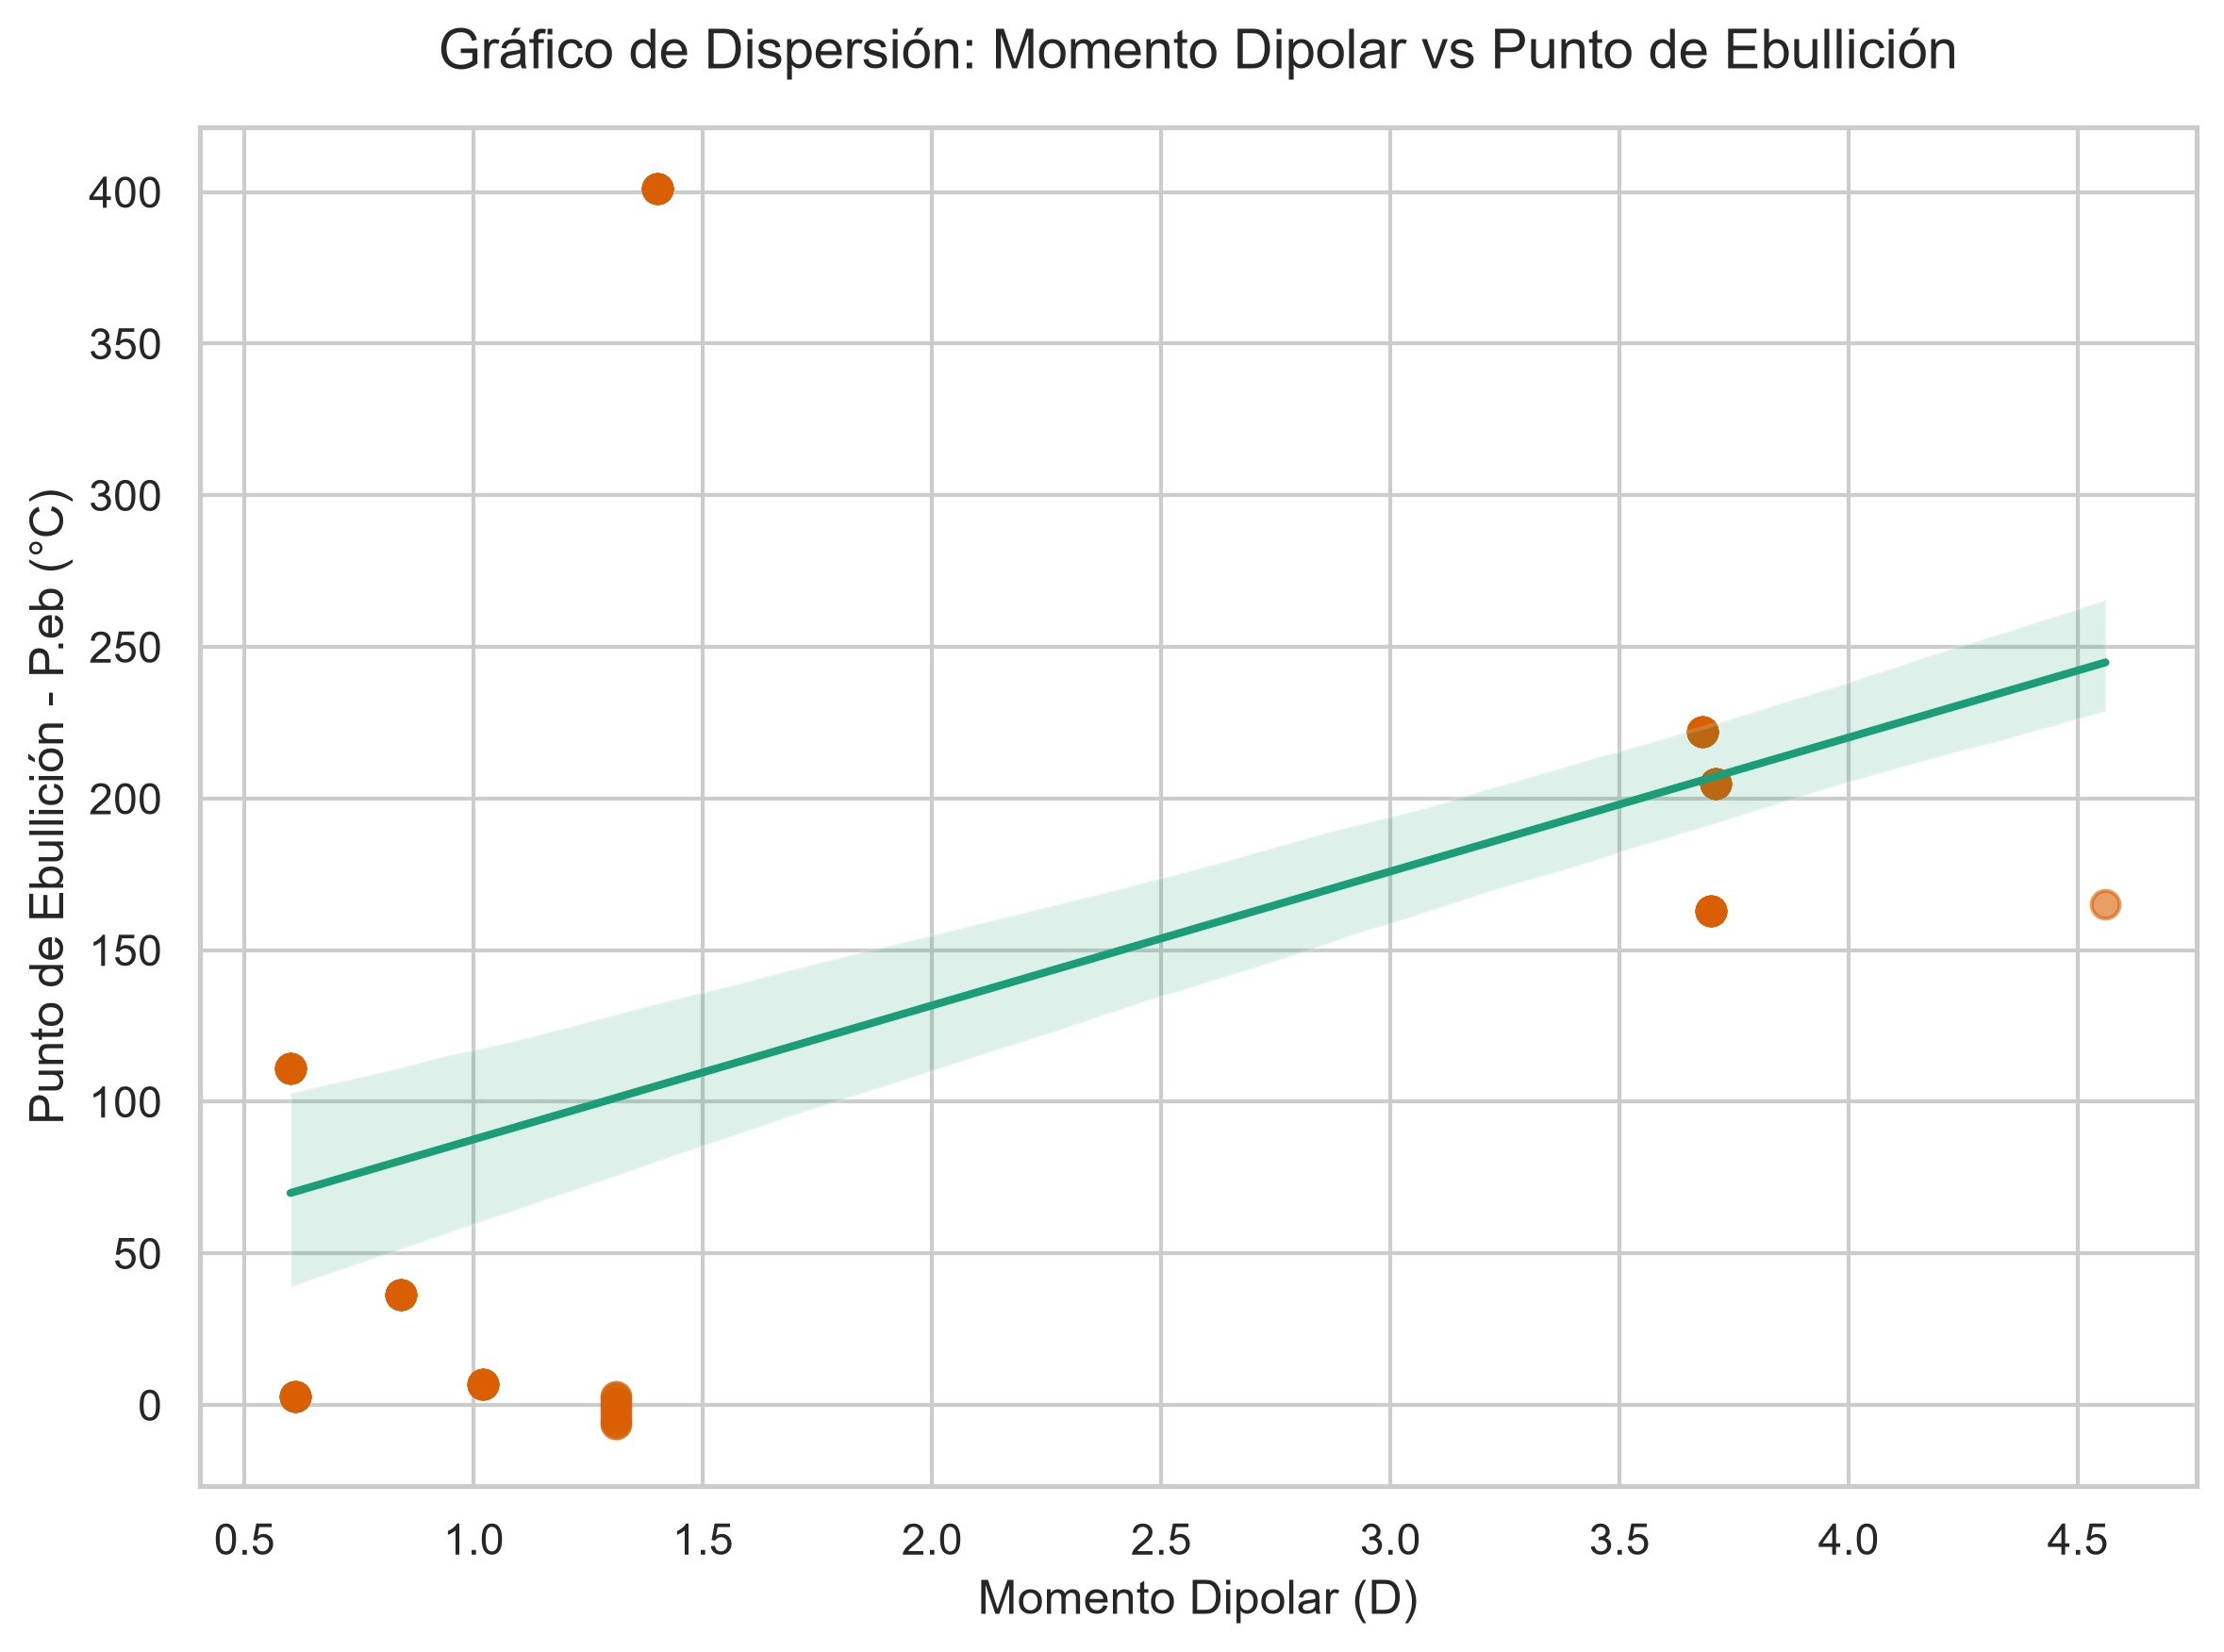
\includegraphics[width=\columnwidth]{06_reg_dipolo_vs_peb.png}
	\caption{Momento dipolar frente a punto de ebullición.}
	\label{fig:dip-peb}
\end{figure}

\subsection{Exploración interactiva con Plotly}
% TODO (Valentina): interpretar; idea central: a igual PM, los compuestos con
% enlace N--H (donadores de puente de H) hierven mucho más alto.
Las Figuras~\ref{fig:burbujas}--\ref{fig:dens-sol} se generaron con Plotly,
una fila por compuesto; sus versiones HTML permiten inspeccionar cada molécula
con el cursor. En la Figura~\ref{fig:burbujas}, trimetilamina
(\SI{2.8}{\degreeCelsius}) y N-metiletanamina (\SI{36.5}{\degreeCelsius}) tienen
el mismo peso molecular (\SI{59.11}{\gram\per\mole}): la diferencia se debe a que
sólo la segunda posee enlace N--H y forma puentes de hidrógeno.
\textit{[Interpretación pendiente.]}

\begin{figure}[htbp]
	\centering
	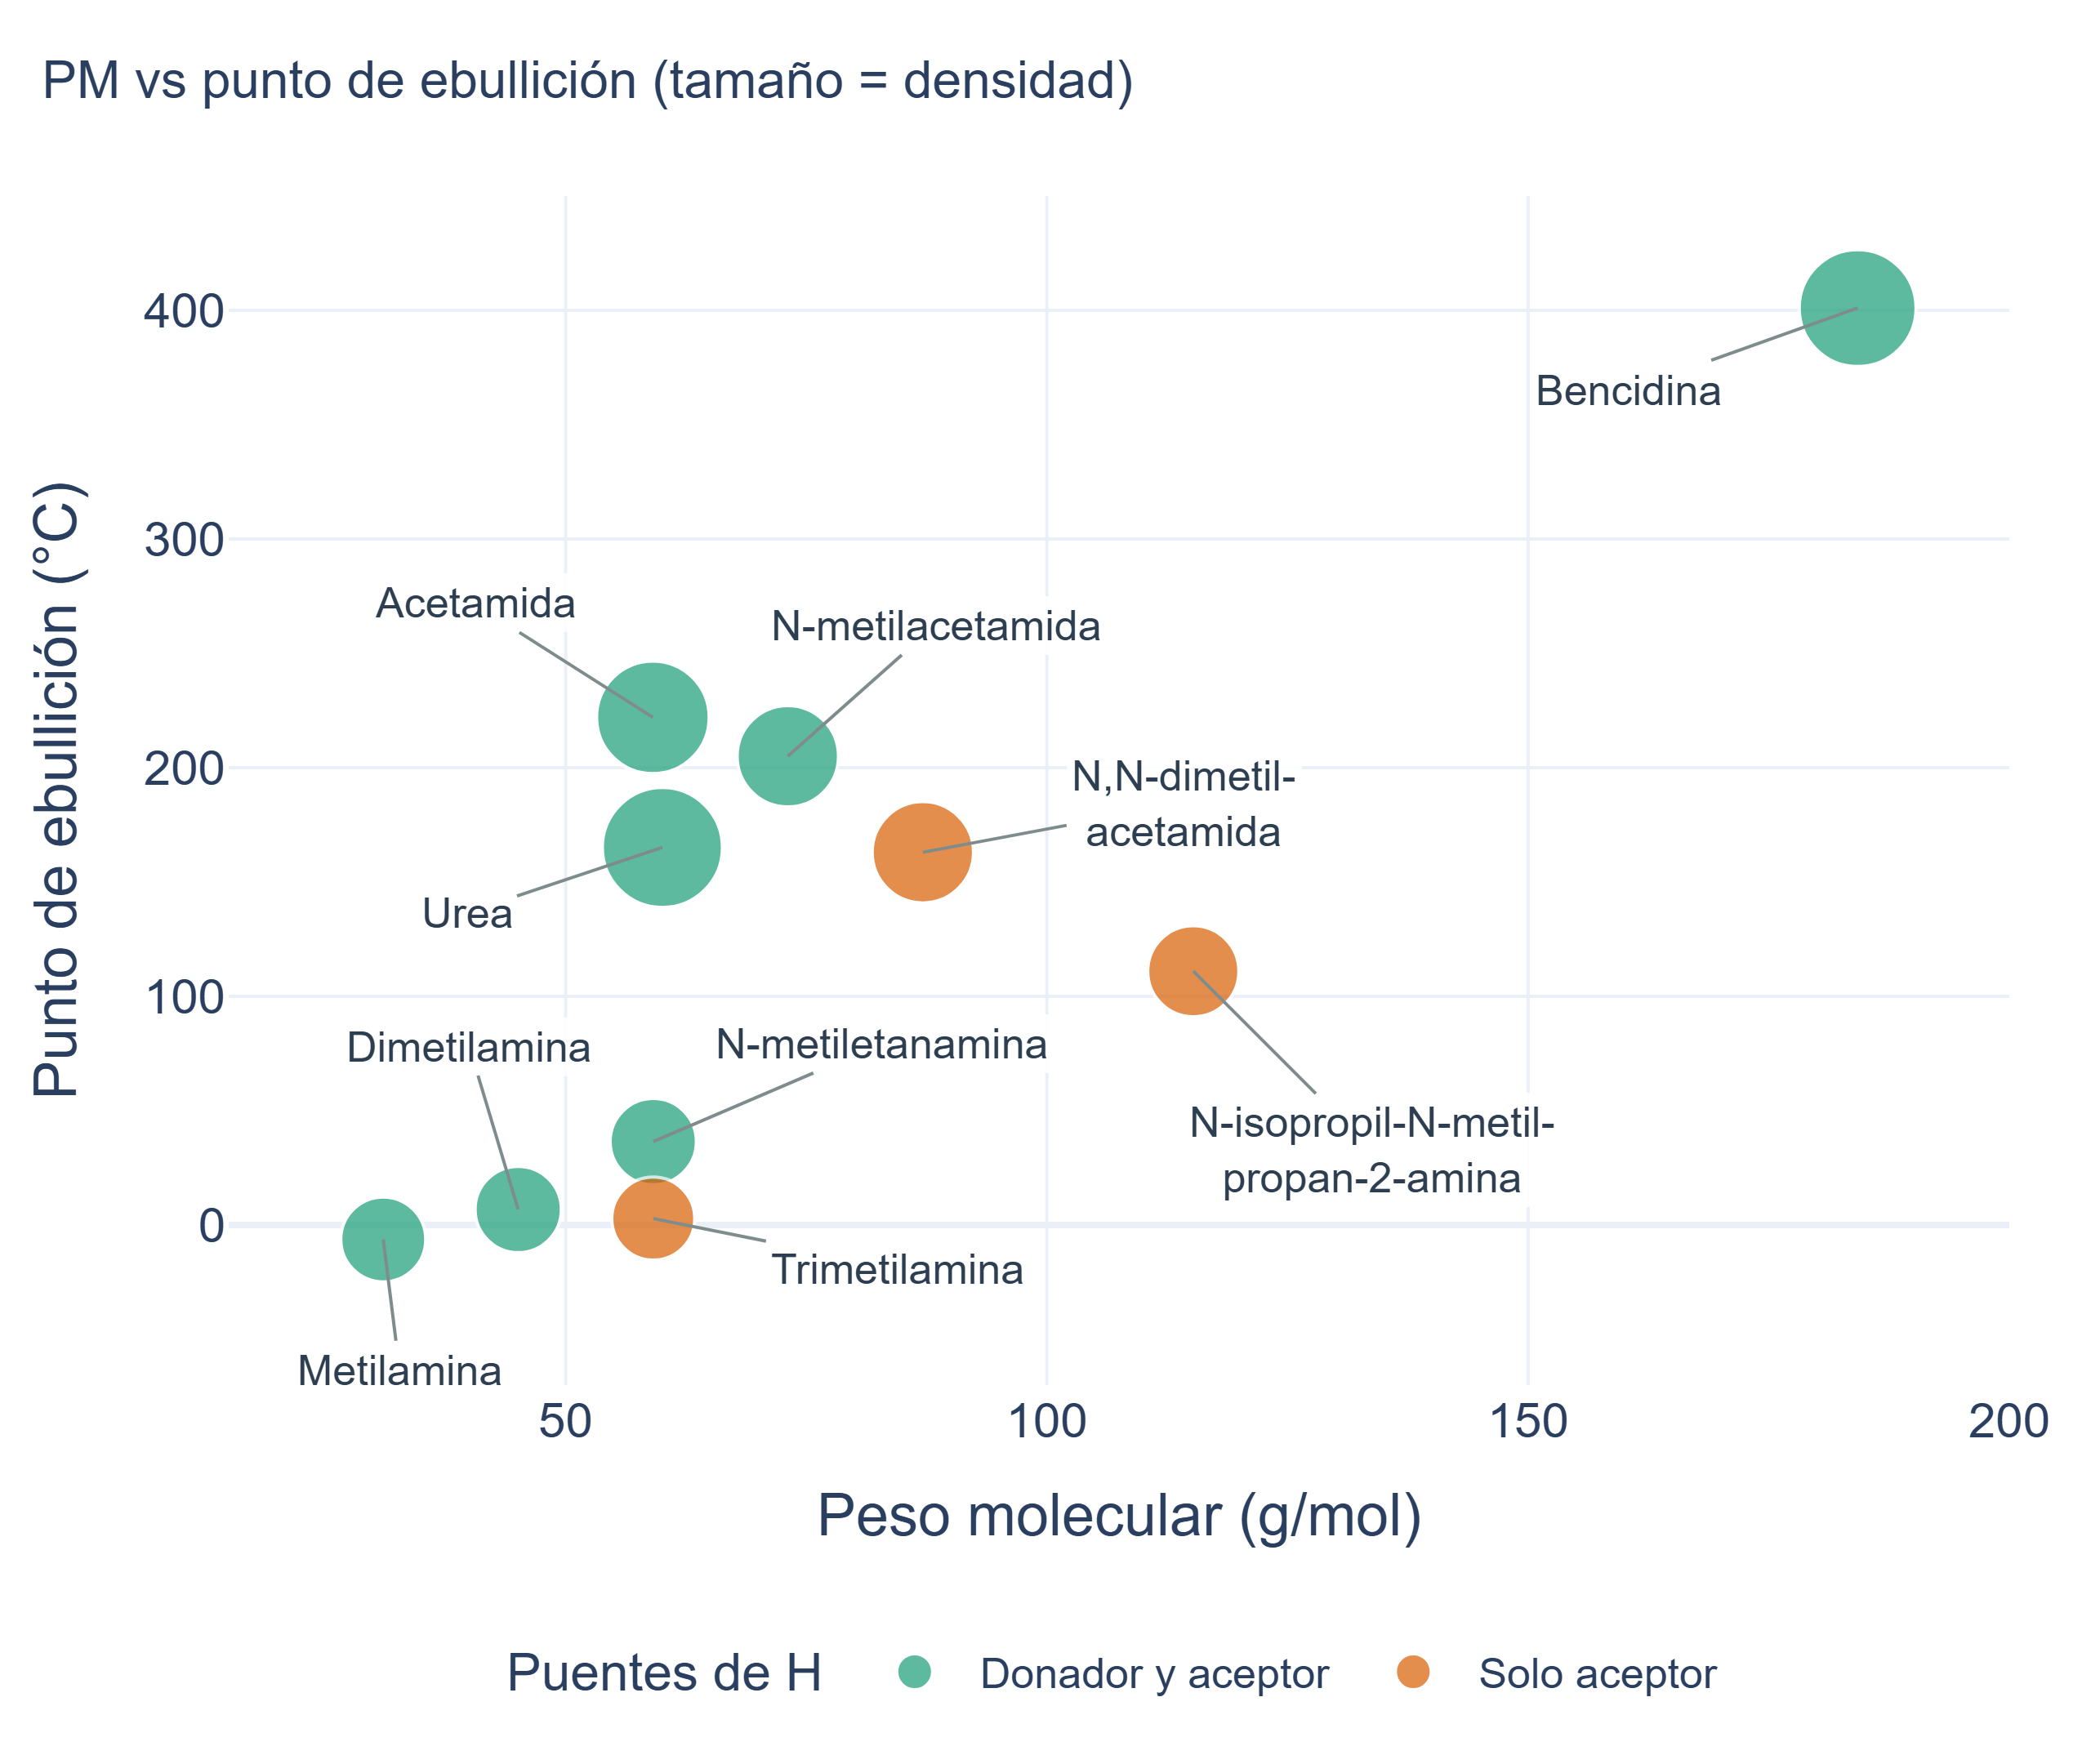
\includegraphics[width=\columnwidth]{11_plotly_burbujas_pm_peb.png}
	\caption{Peso molecular frente a punto de ebullición; el tamaño representa la densidad y el color la capacidad de formar puentes de hidrógeno.}
	\label{fig:burbujas}
\end{figure}

\begin{figure}[htbp]
	\centering
	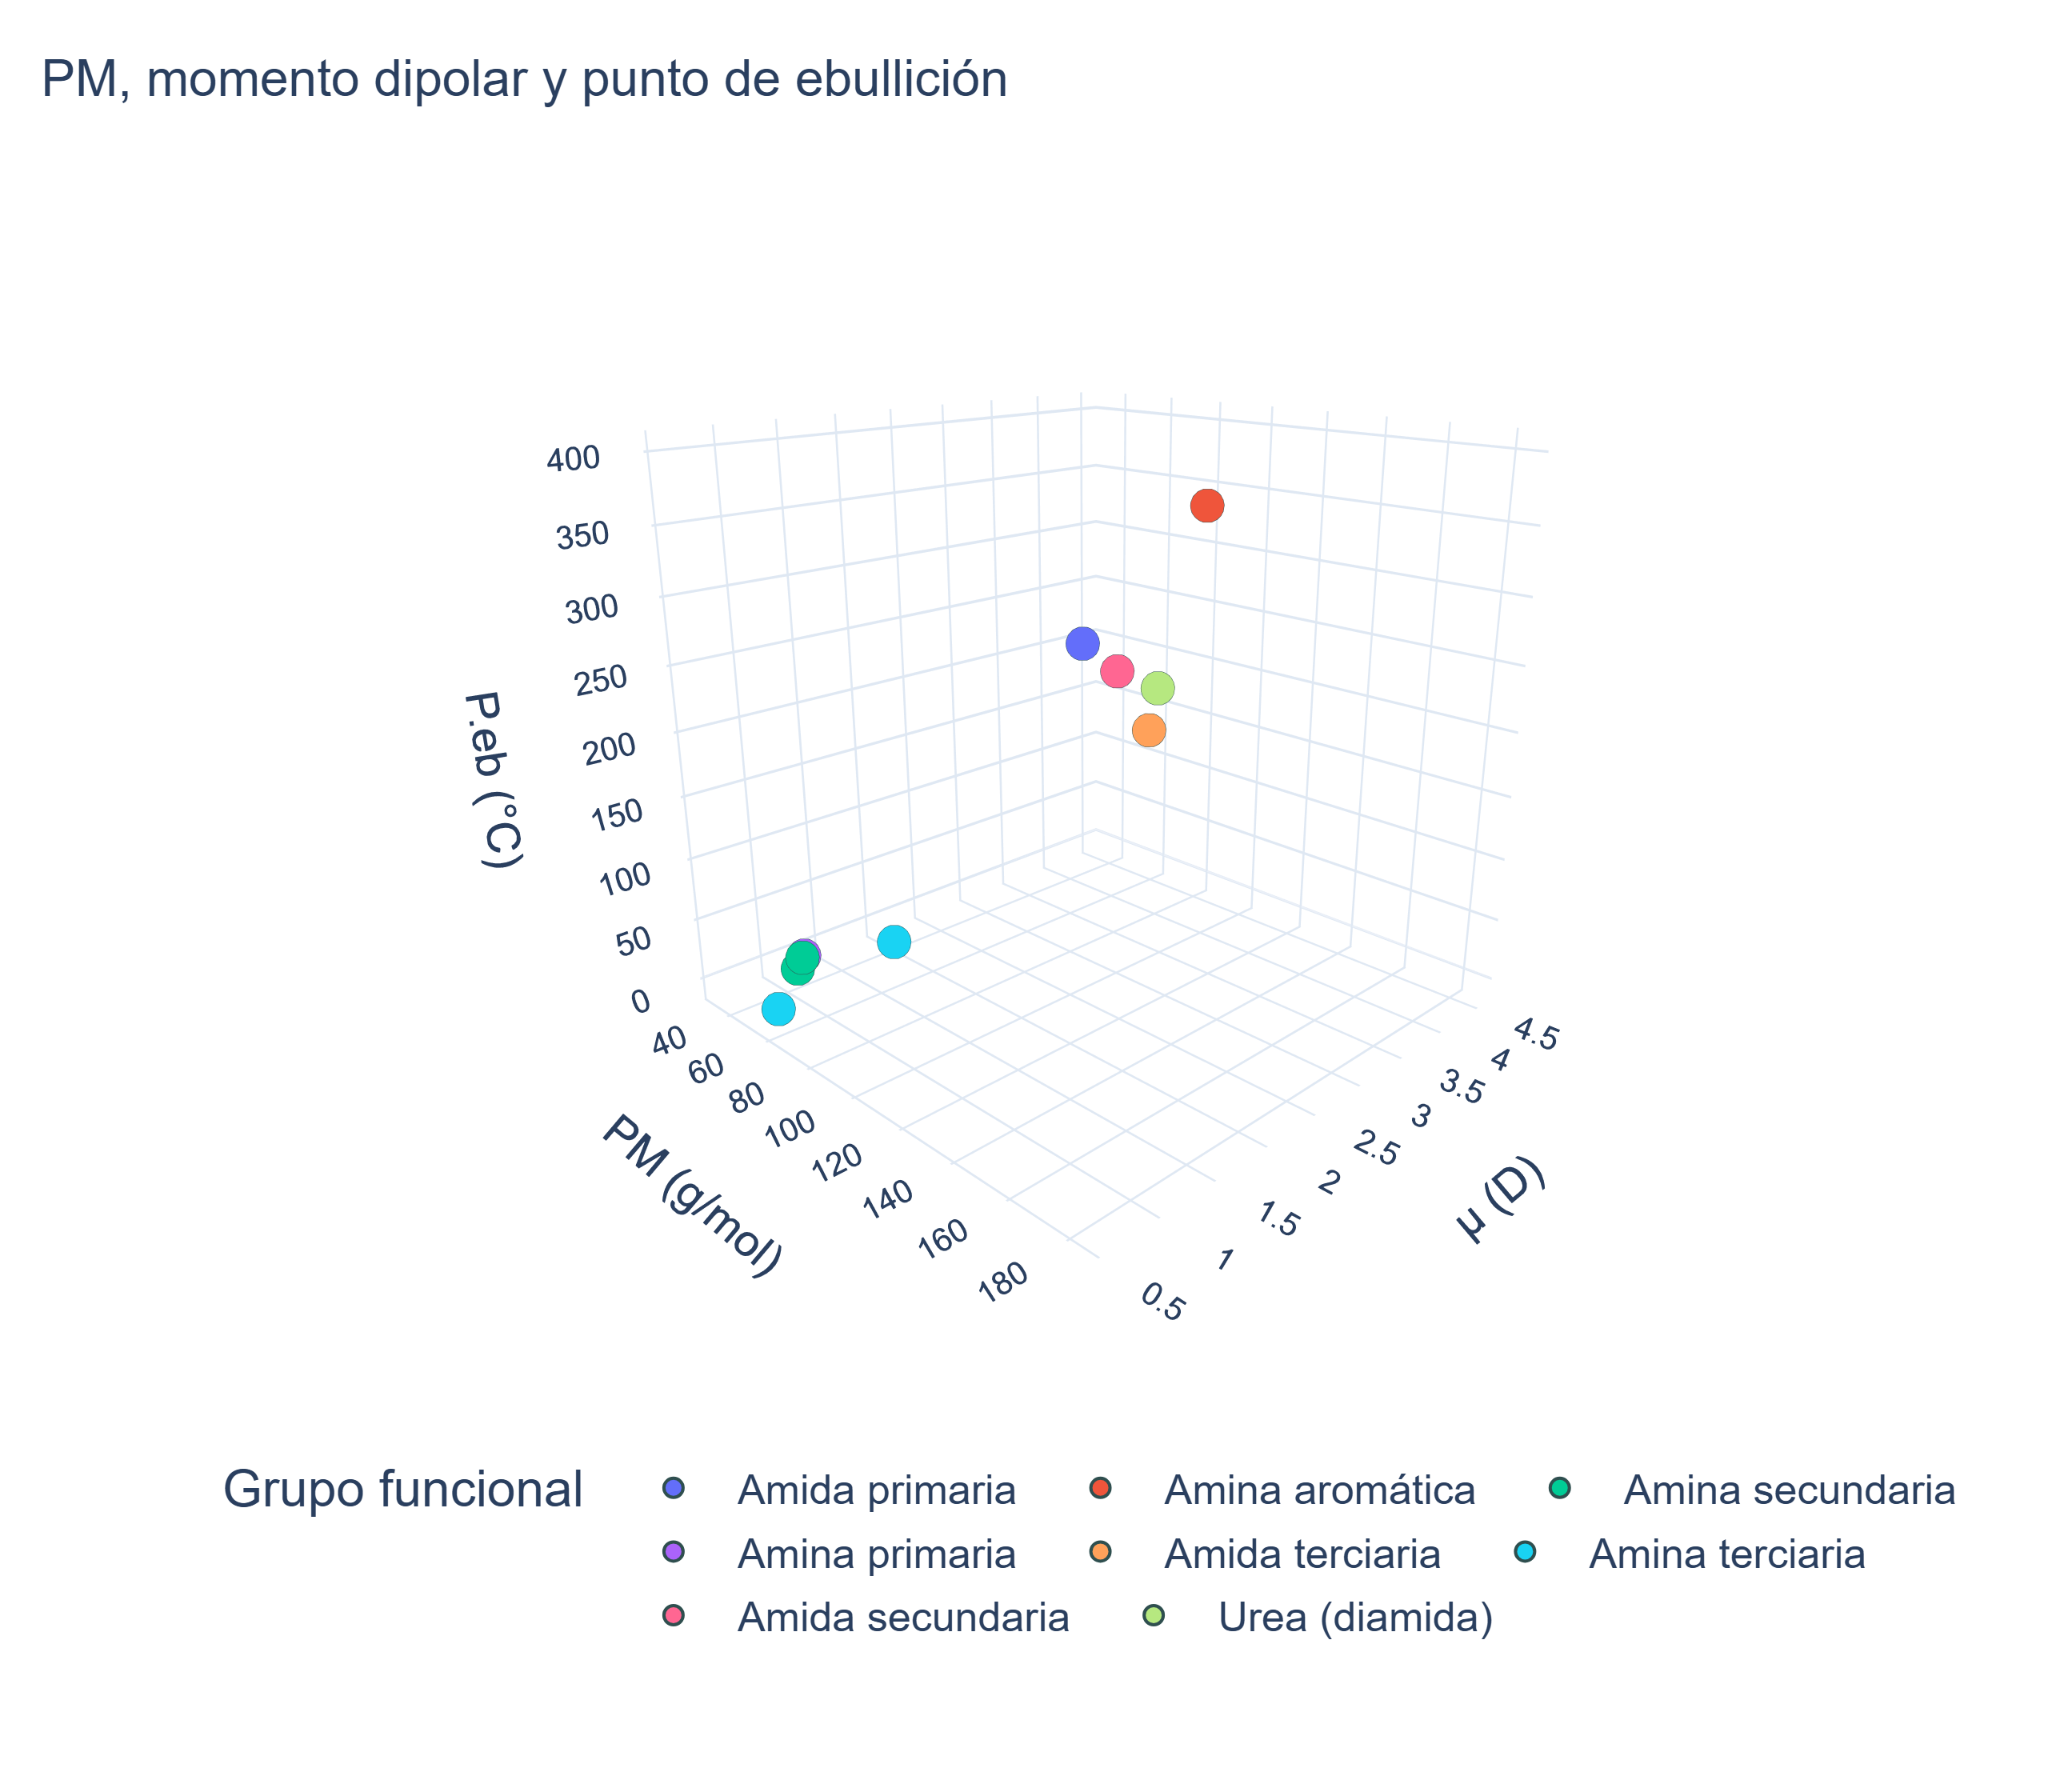
\includegraphics[width=\columnwidth]{12_plotly_3d_pm_dipolo_peb.png}
	\caption{Espacio tridimensional de peso molecular, momento dipolar y punto de ebullición por grupo funcional.}
	\label{fig:3d}
\end{figure}

\begin{figure}[htbp]
	\centering
	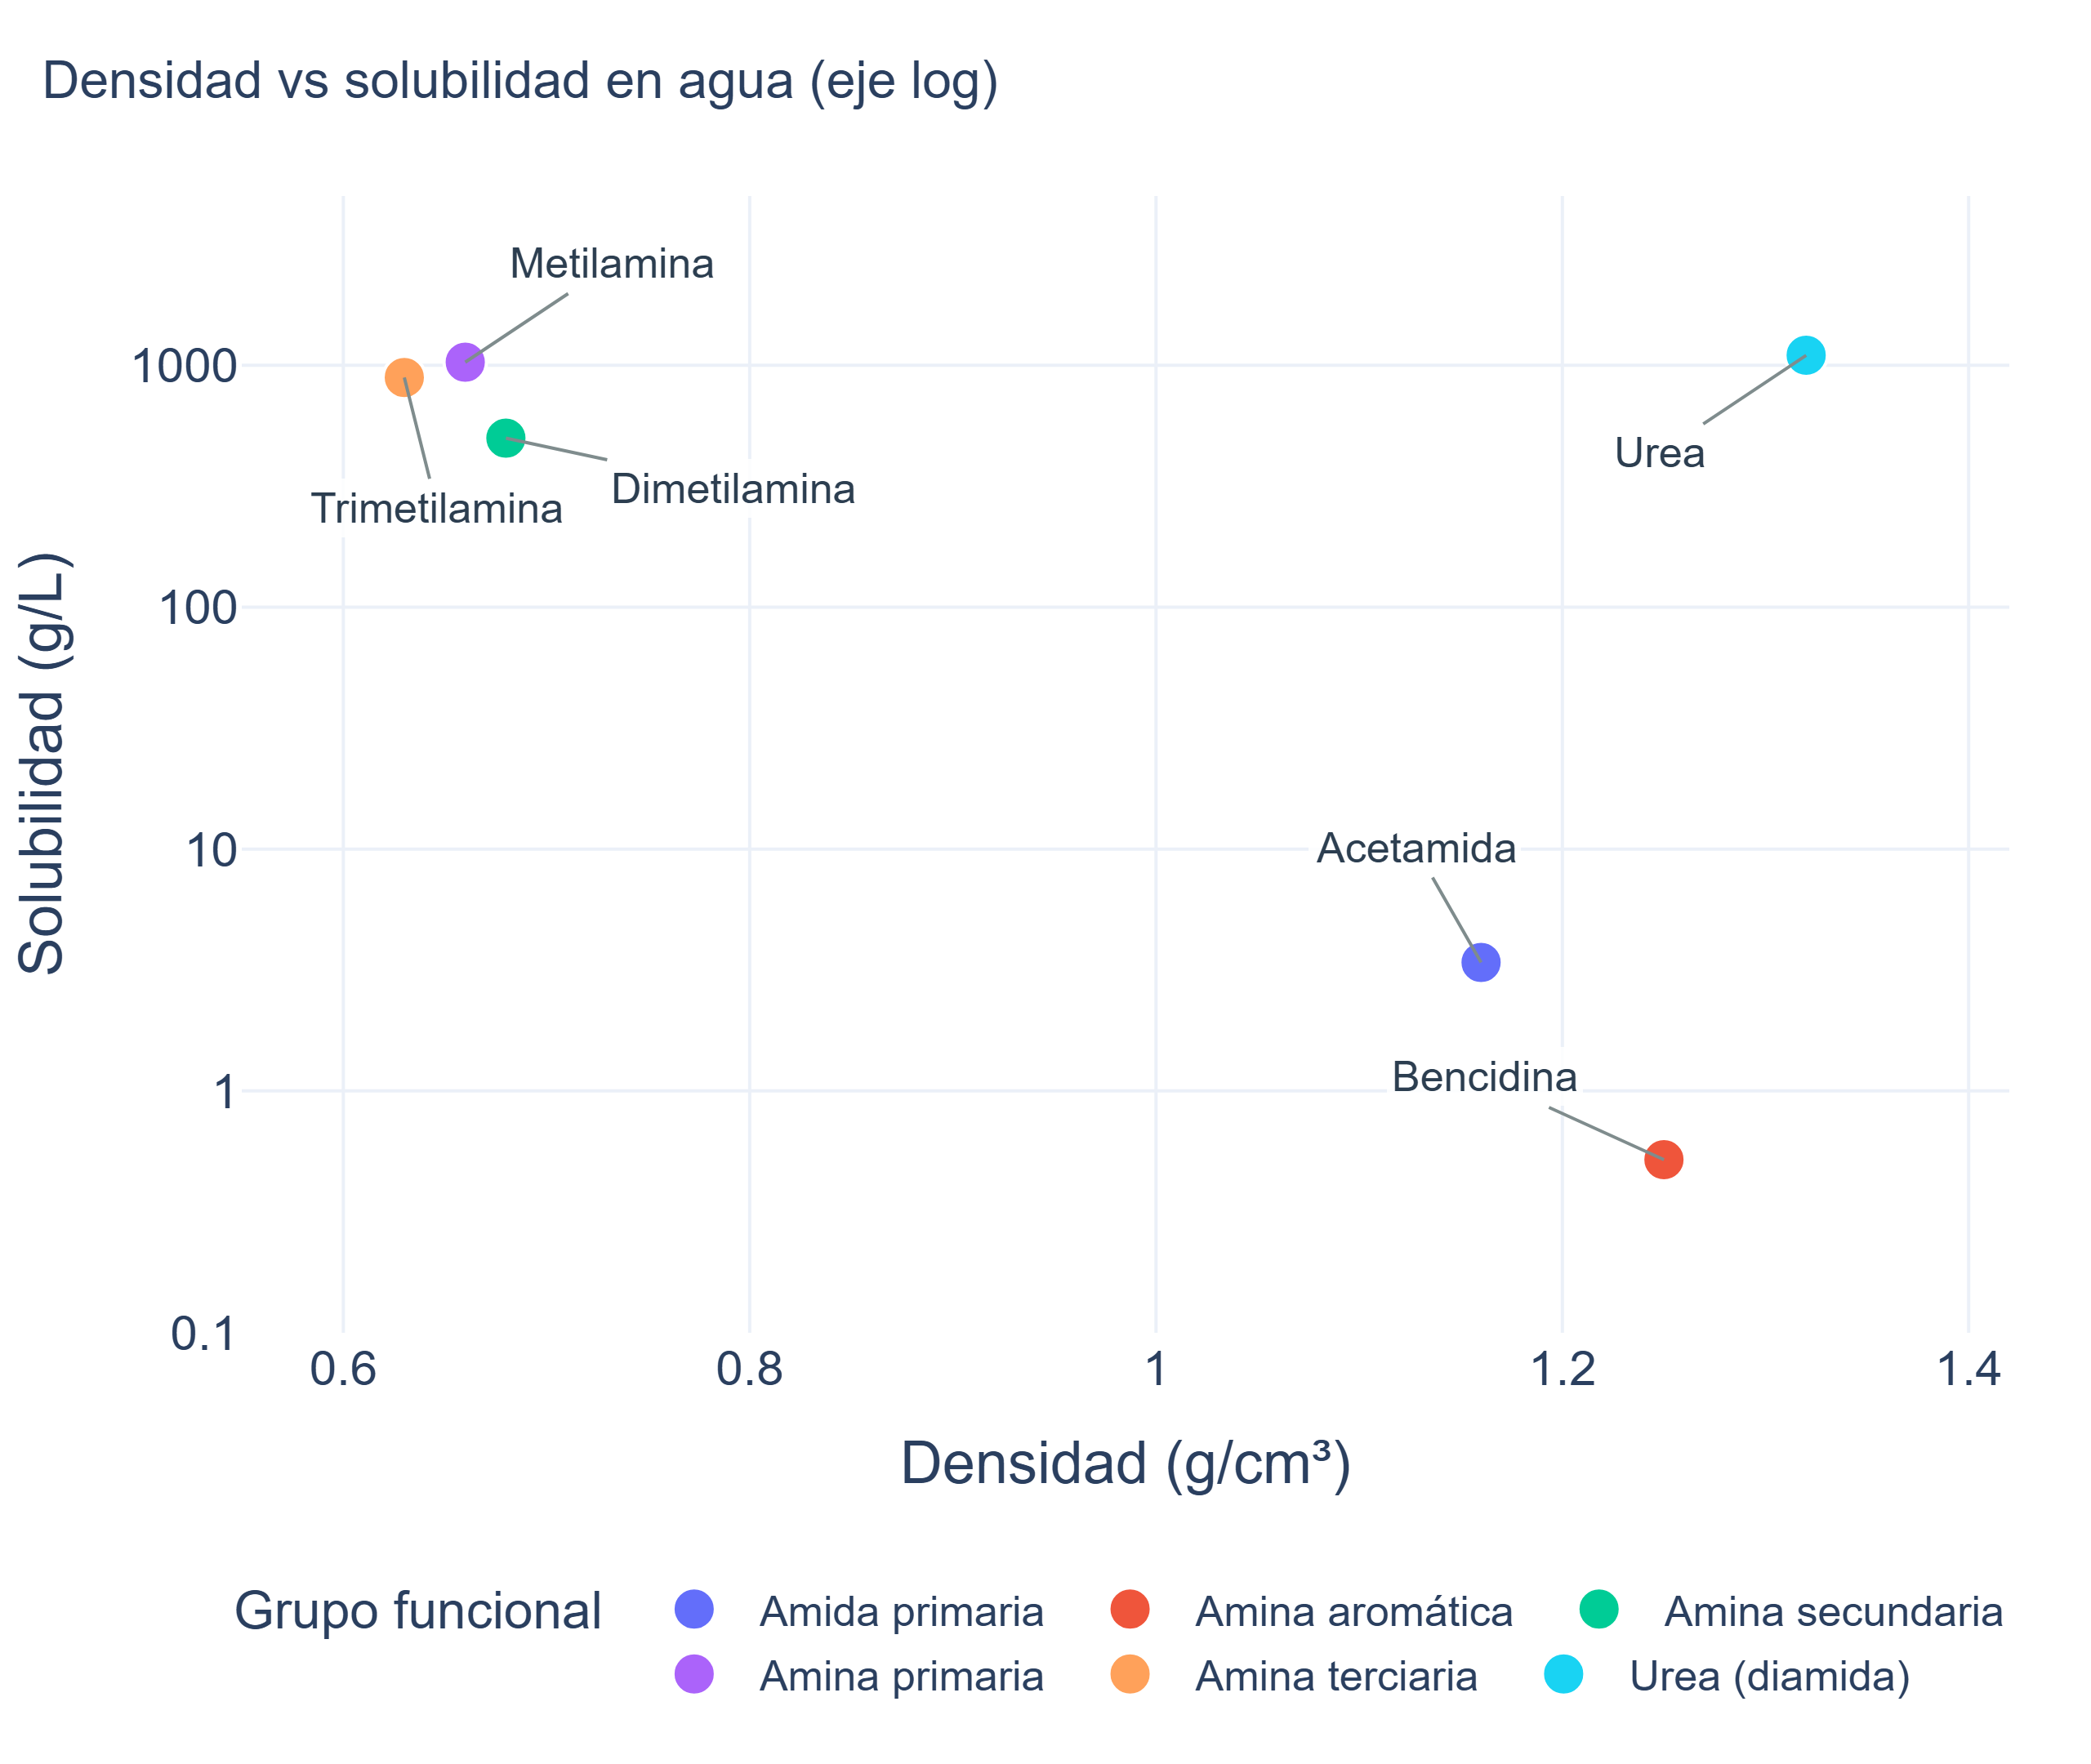
\includegraphics[width=\columnwidth]{13_plotly_densidad_solubilidad.png}
	\caption{Densidad frente a solubilidad en agua (eje logarítmico).}
	\label{fig:dens-sol}
\end{figure}

\subsection{Distribución por tipo de reacción y medio}
% TODO (Valentina): explicar qué representa TR y comparar medianas/dispersiones.
La Figura~\ref{fig:frecuencias} compara la frecuencia de cada mecanismo de
reacción y de cada medio; la sustitución nucleofílica (SN) domina, coherente con
el carácter nucleófilo del par libre del nitrógeno. Las
Figuras~\ref{fig:violin}--\ref{fig:dona} describen la distribución de
probabilidad de TR según el tipo de reacción y el medio.
\textit{[Interpretación pendiente.]}

\begin{figure}[htbp]
	\centering
	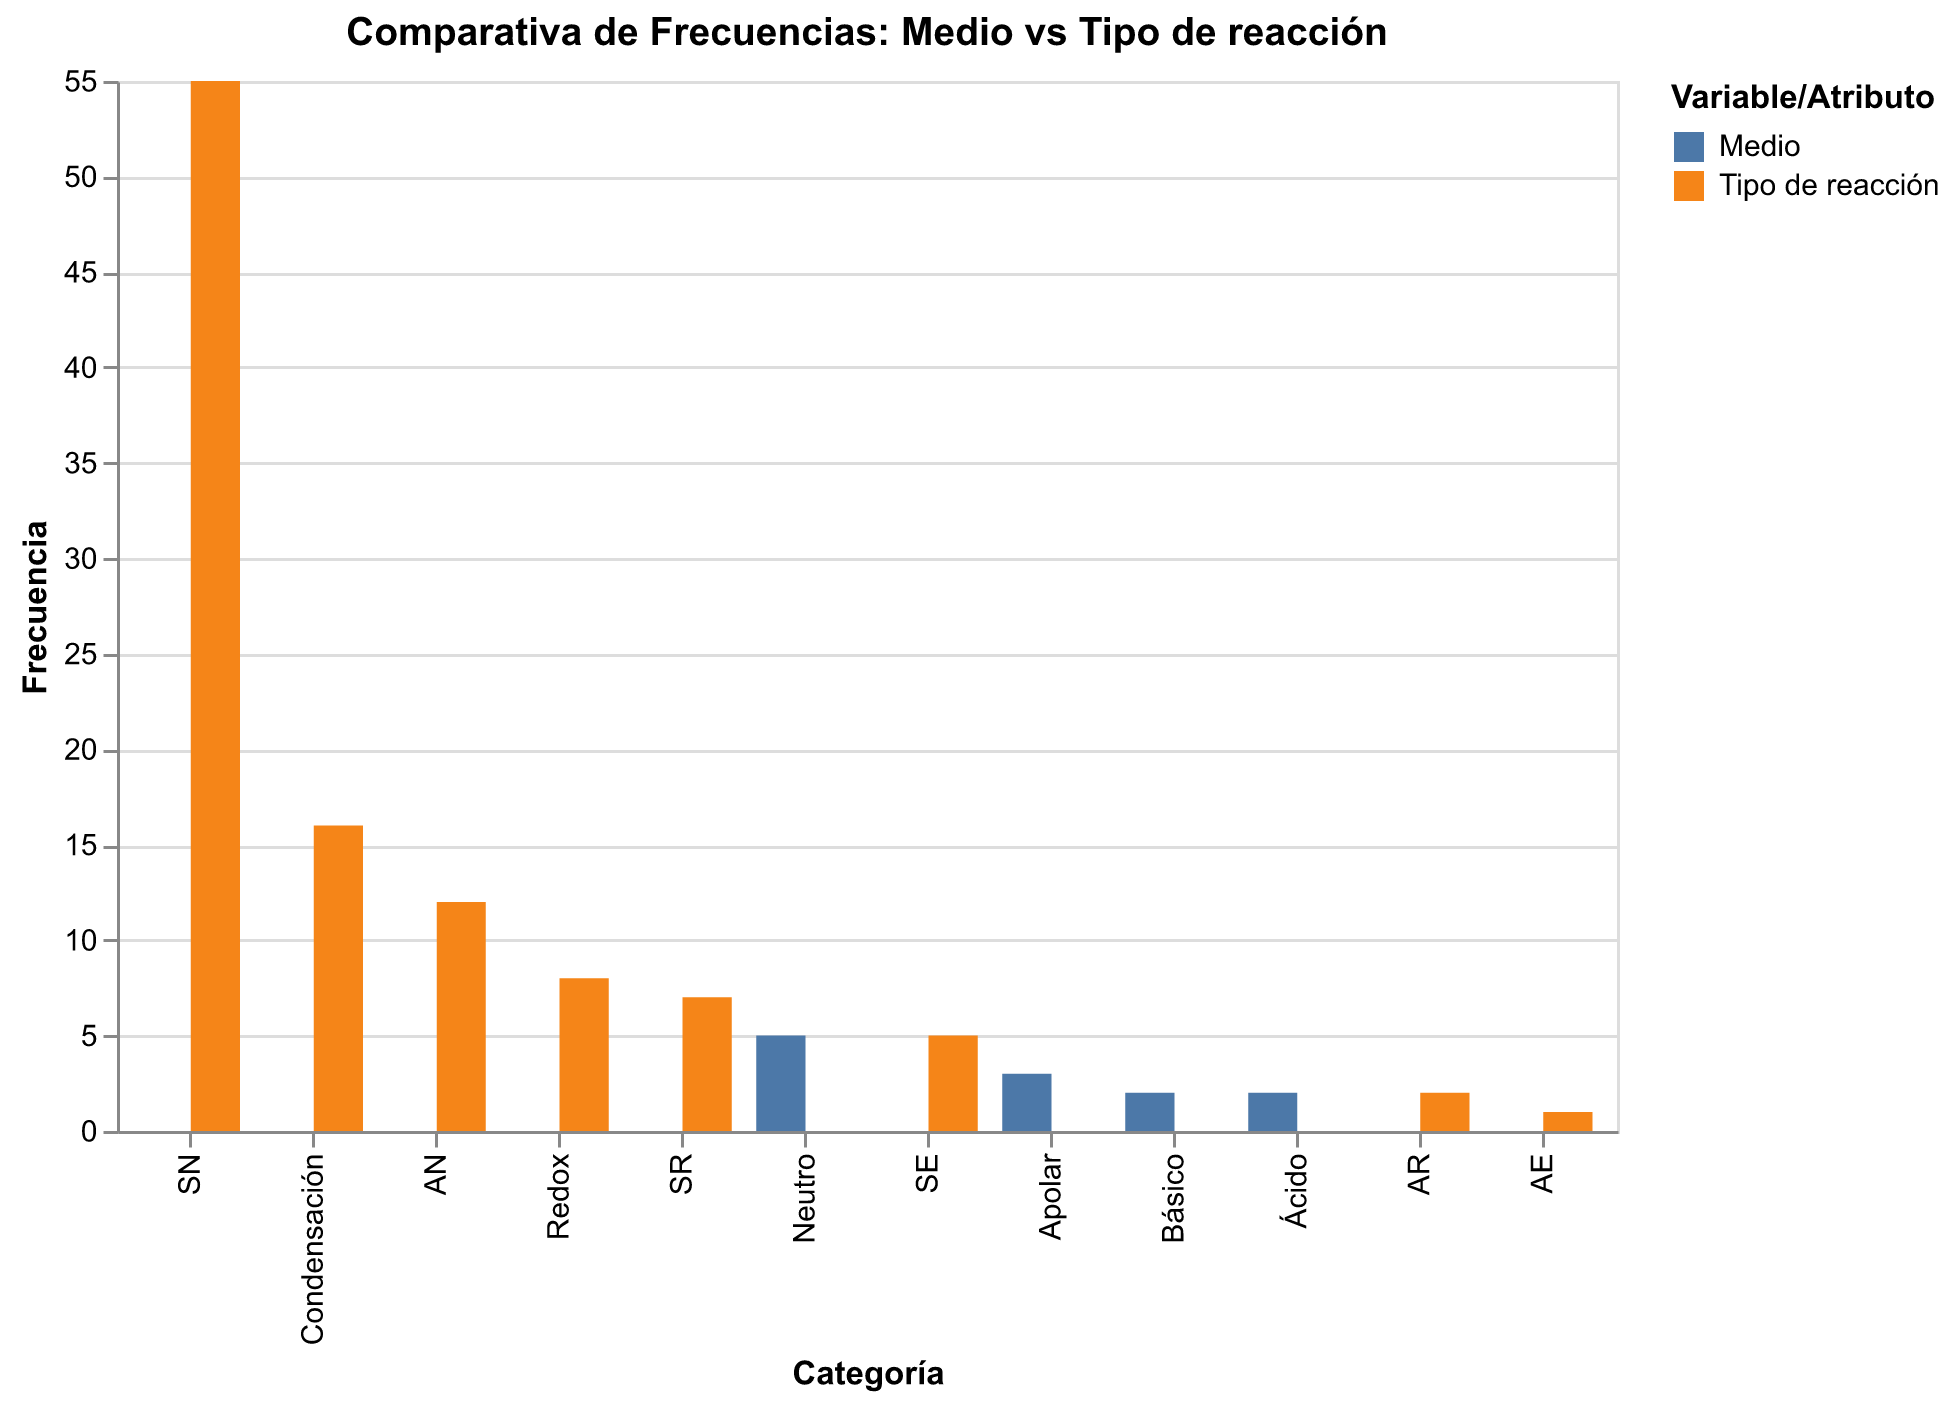
\includegraphics[width=\columnwidth]{09_frecuencias_medio_tipo.png}
	\caption{Frecuencia de los tipos de reacción y de los medios reportados.}
	\label{fig:frecuencias}
\end{figure}

\begin{figure}[htbp]
	\centering
	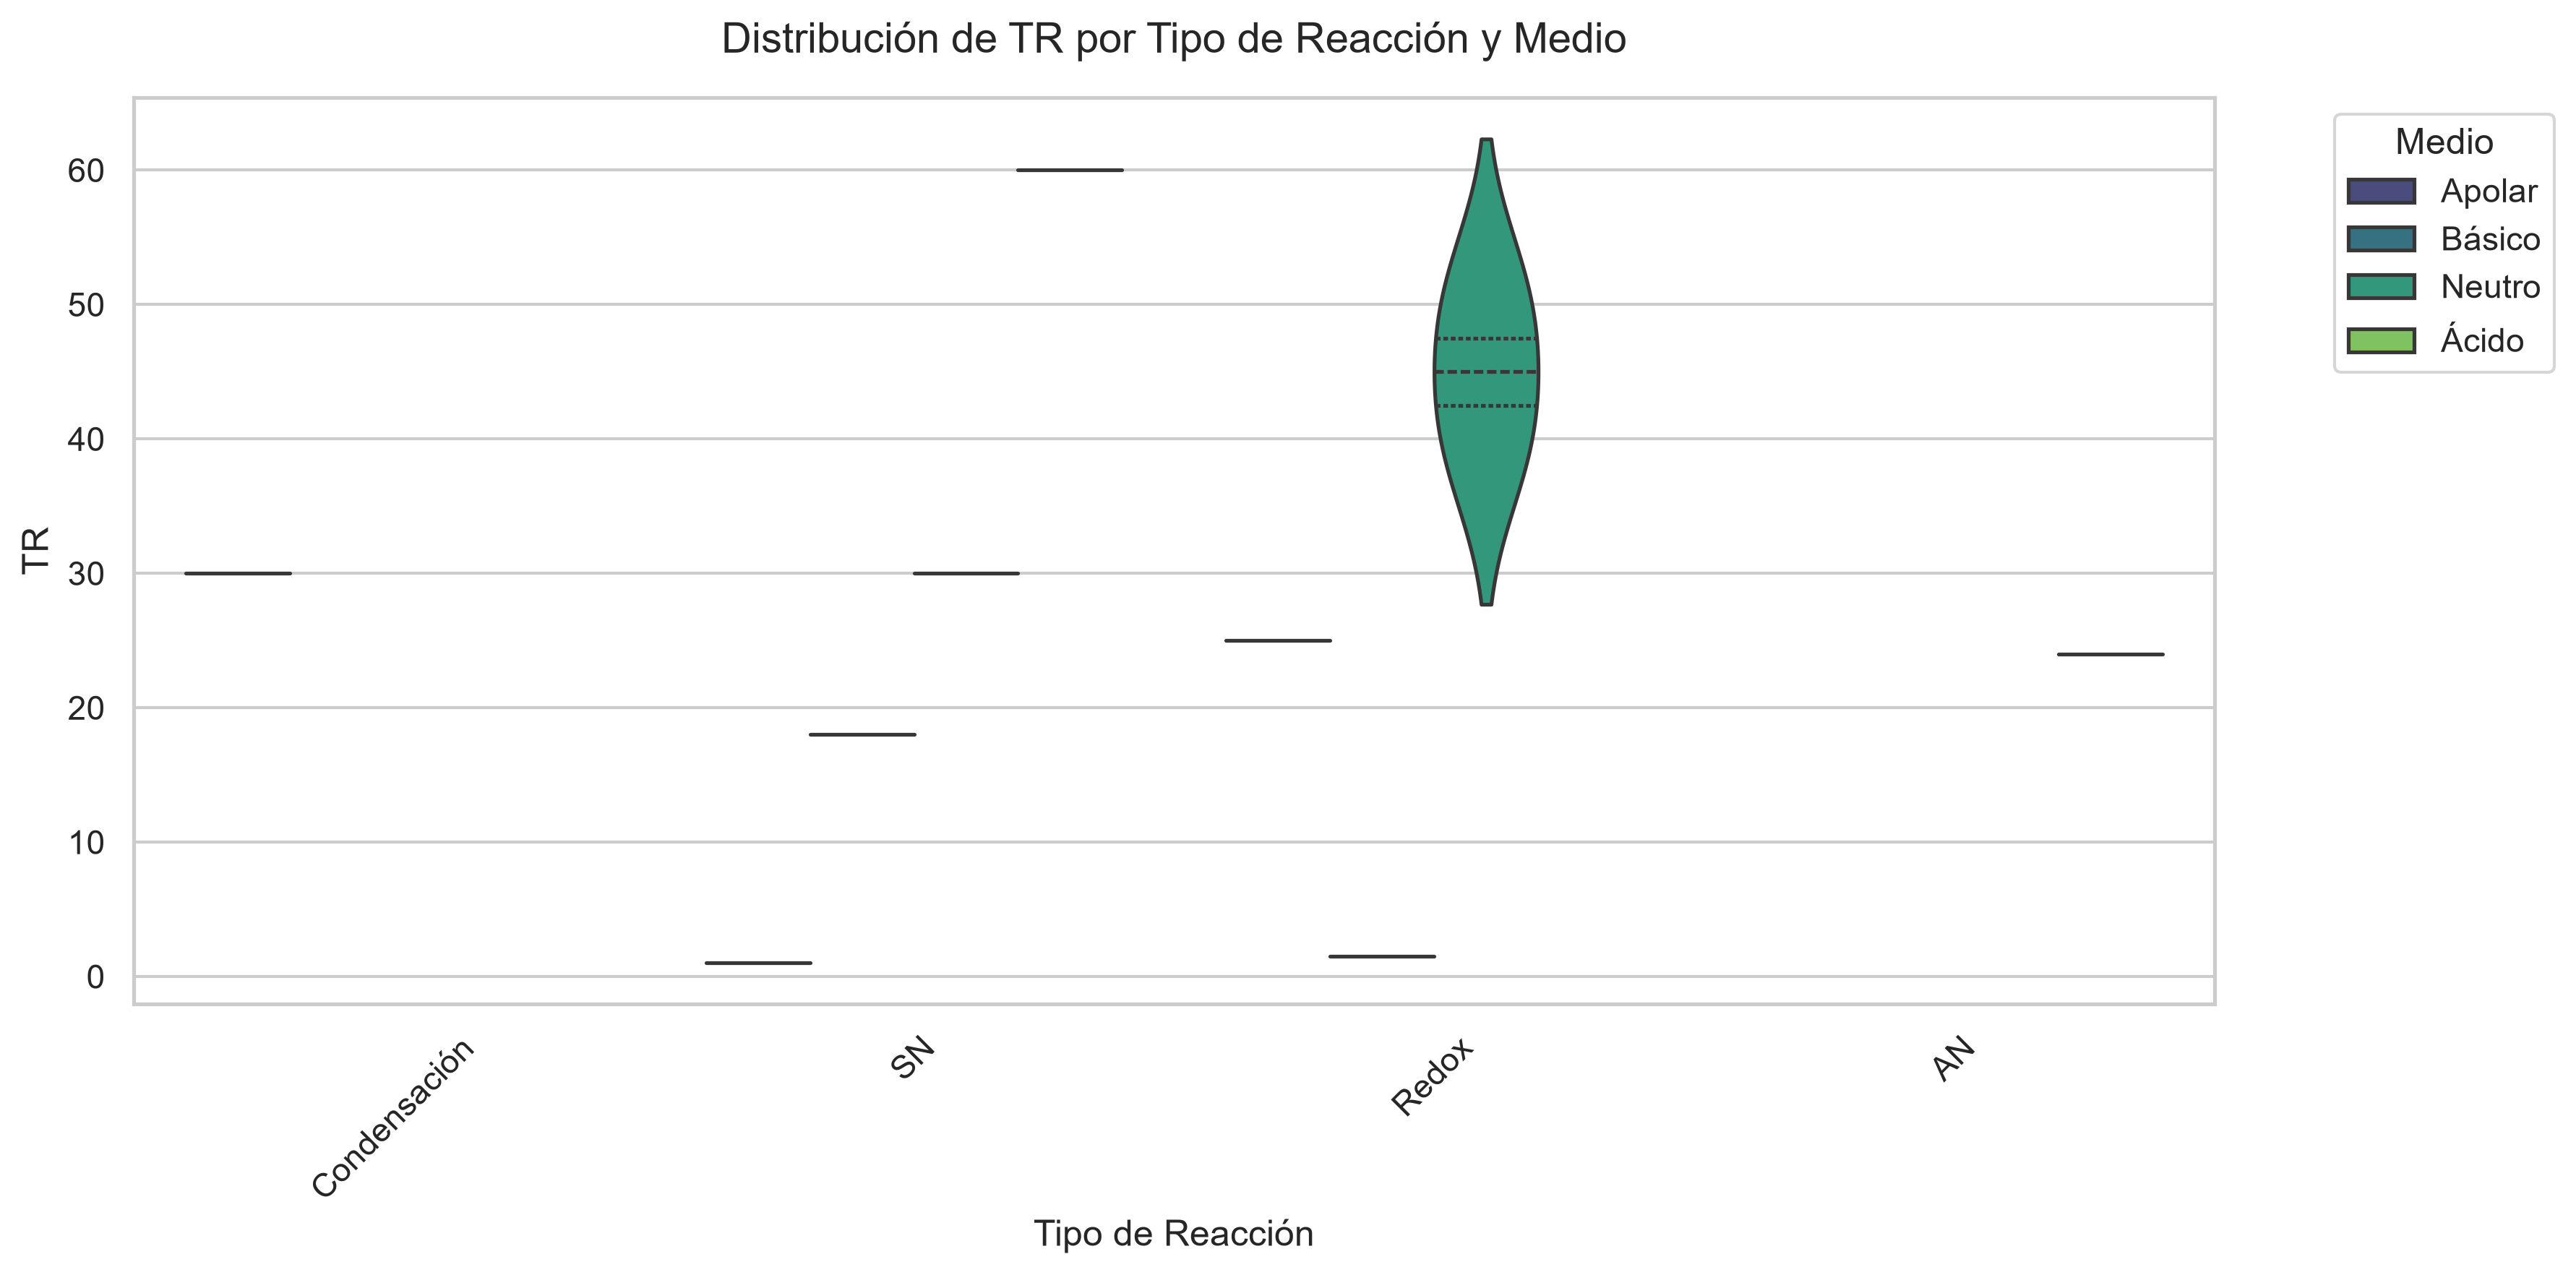
\includegraphics[width=\columnwidth]{07_violin_TR_tipo_medio.png}
	\caption{Distribución (violín) de TR por tipo de reacción y medio.}
	\label{fig:violin}
\end{figure}

\begin{figure}[htbp]
	\centering
	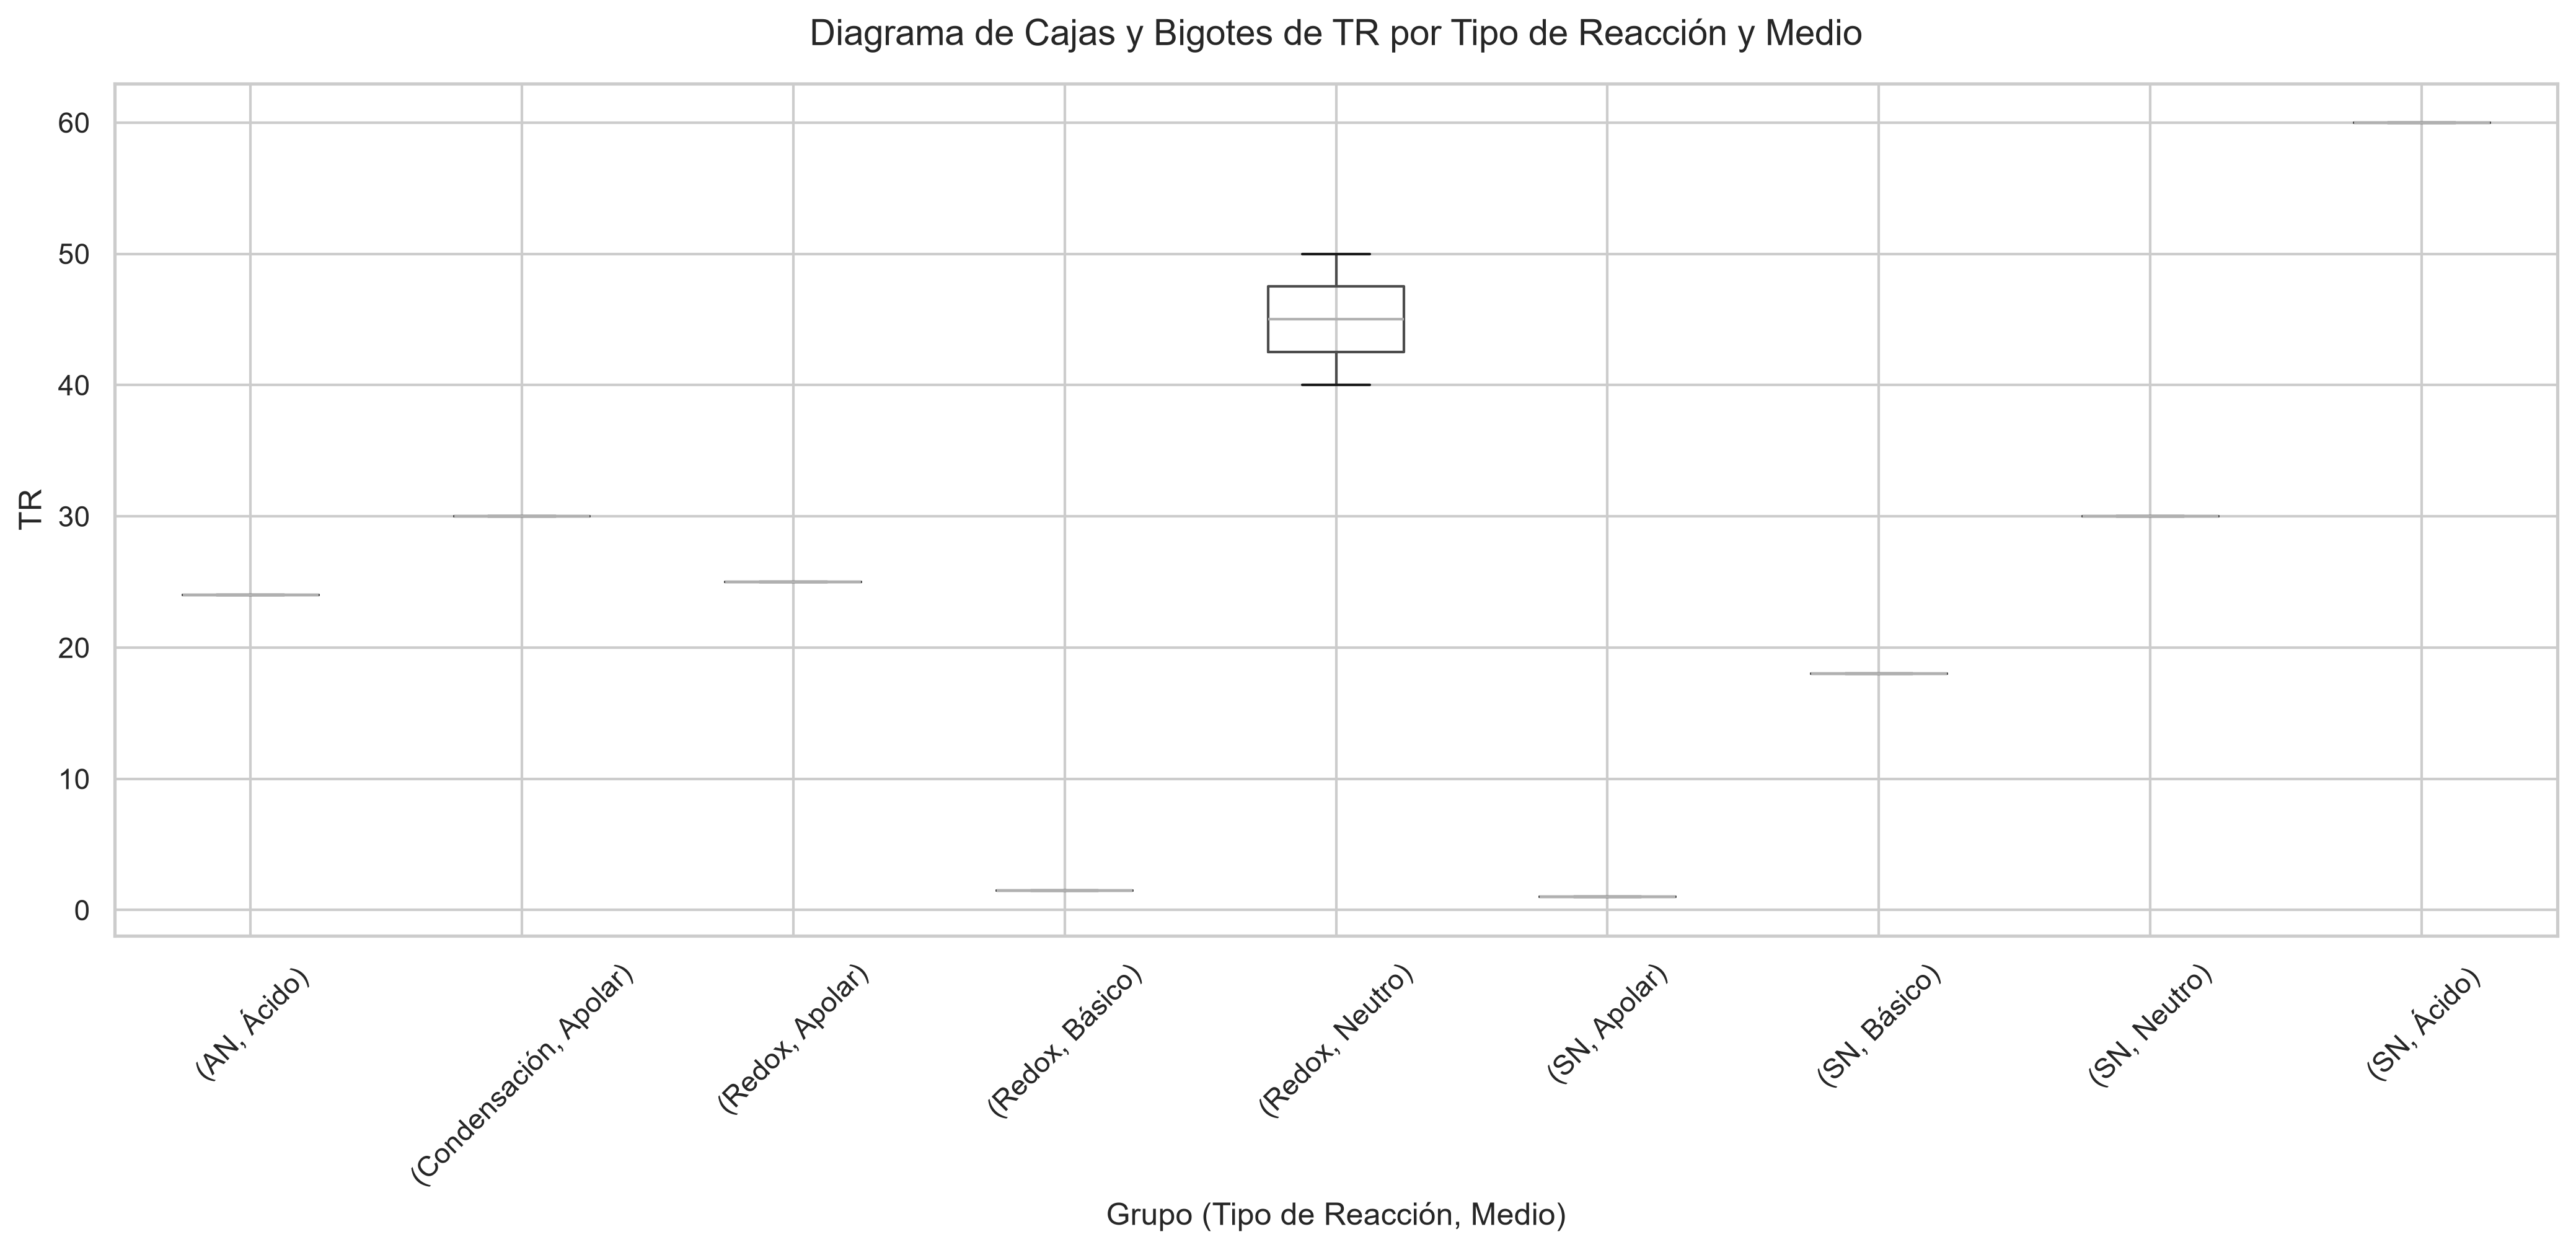
\includegraphics[width=\columnwidth]{08_boxplot_TR_tipo_medio.png}
	\caption{Diagrama de cajas y bigotes de TR por tipo de reacción y medio.}
	\label{fig:boxplot}
\end{figure}

\begin{figure}[htbp]
	\centering
	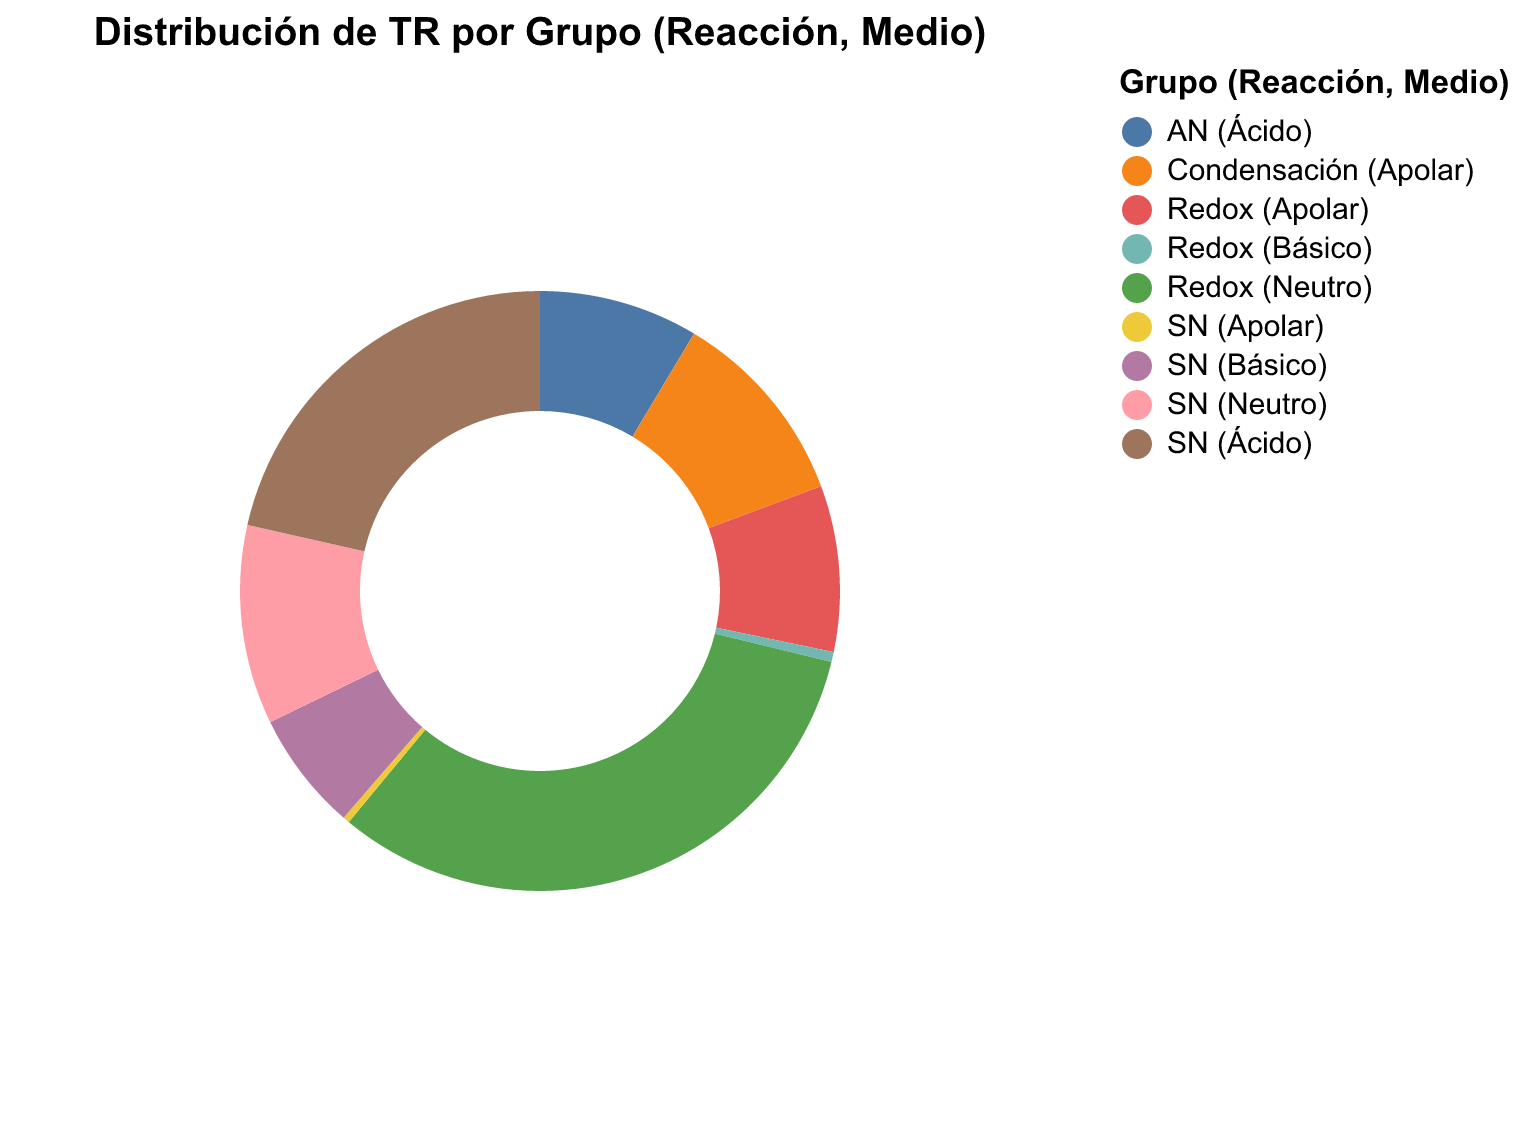
\includegraphics[width=0.9\columnwidth]{10_dona_TR_grupo.png}
	\caption{Participación de TR por grupo (tipo de reacción, medio).}
	\label{fig:dona}
\end{figure}

\section{Conclusiones y Perspectiva}
\fontsize{12}{14}\selectfont
% TODO (Valentina): 3--5 conclusiones que respondan al objetivo de la introducción,
% cada una sustentada en una figura o en la Tabla~\ref{tab:propiedades}.
\textit{[Redacción pendiente.]}

%  Contenido: Metodología, Análisis Gráfico (Colab/Conda) y Conclusiones
%
%  Reglas para editar sin romper la compilación:
%   * NO escribir \documentclass, \begin{document} ni \end{document} aquí.
%   * Las figuras están en ../imagenes/ y se llaman sólo por su nombre
%     (main.tex ya define \graphicspath{{imagenes/}}).
%   * Referenciar figuras con Figura~\ref{fig:...}, nunca "la figura de abajo".
% =====================================================================

\section{Metodología}
\fontsize{12}{14}\selectfont
% TODO (Valentina): pegar aquí la redacción de la metodología.

\subsection{Recolección de datos}
\textit{[Redacción pendiente: búsqueda en CAS-SciFinder, compuestos e indicadores asignados, consolidación en Excel con formato Tabla.]}

\subsection{Limpieza y procesamiento en Python}
\textit{[Redacción pendiente: Google Colab con Pandas, NumPy, Matplotlib, Seaborn y Plotly; filtrado de los compuestos de interés, conversión de comas decimales, tratamiento de valores nulos y atípicos.]}

\subsection{Análisis estadístico}
\textit{[Redacción pendiente: correlación de Spearman (no paramétrica, robusta a valores atípicos y relaciones monótonas no lineales), regresiones lineales con intervalo de confianza del 95\,\% y distribuciones por tipo de reacción y medio.]}

\section{Resultados y Discusión}
\fontsize{12}{14}\selectfont

\subsection{Correlación entre propiedades}
% TODO (Valentina): interpretar los coeficientes más fuertes (positivos y negativos).
La Figura~\ref{fig:heatmap} presenta la matriz de correlación de Spearman entre
las propiedades fisicoquímicas, y la Figura~\ref{fig:clustermap} agrupa
jerárquicamente las variables con comportamiento similar.
\textit{[Interpretación pendiente.]}

\begin{figure}[htbp]
	\centering
	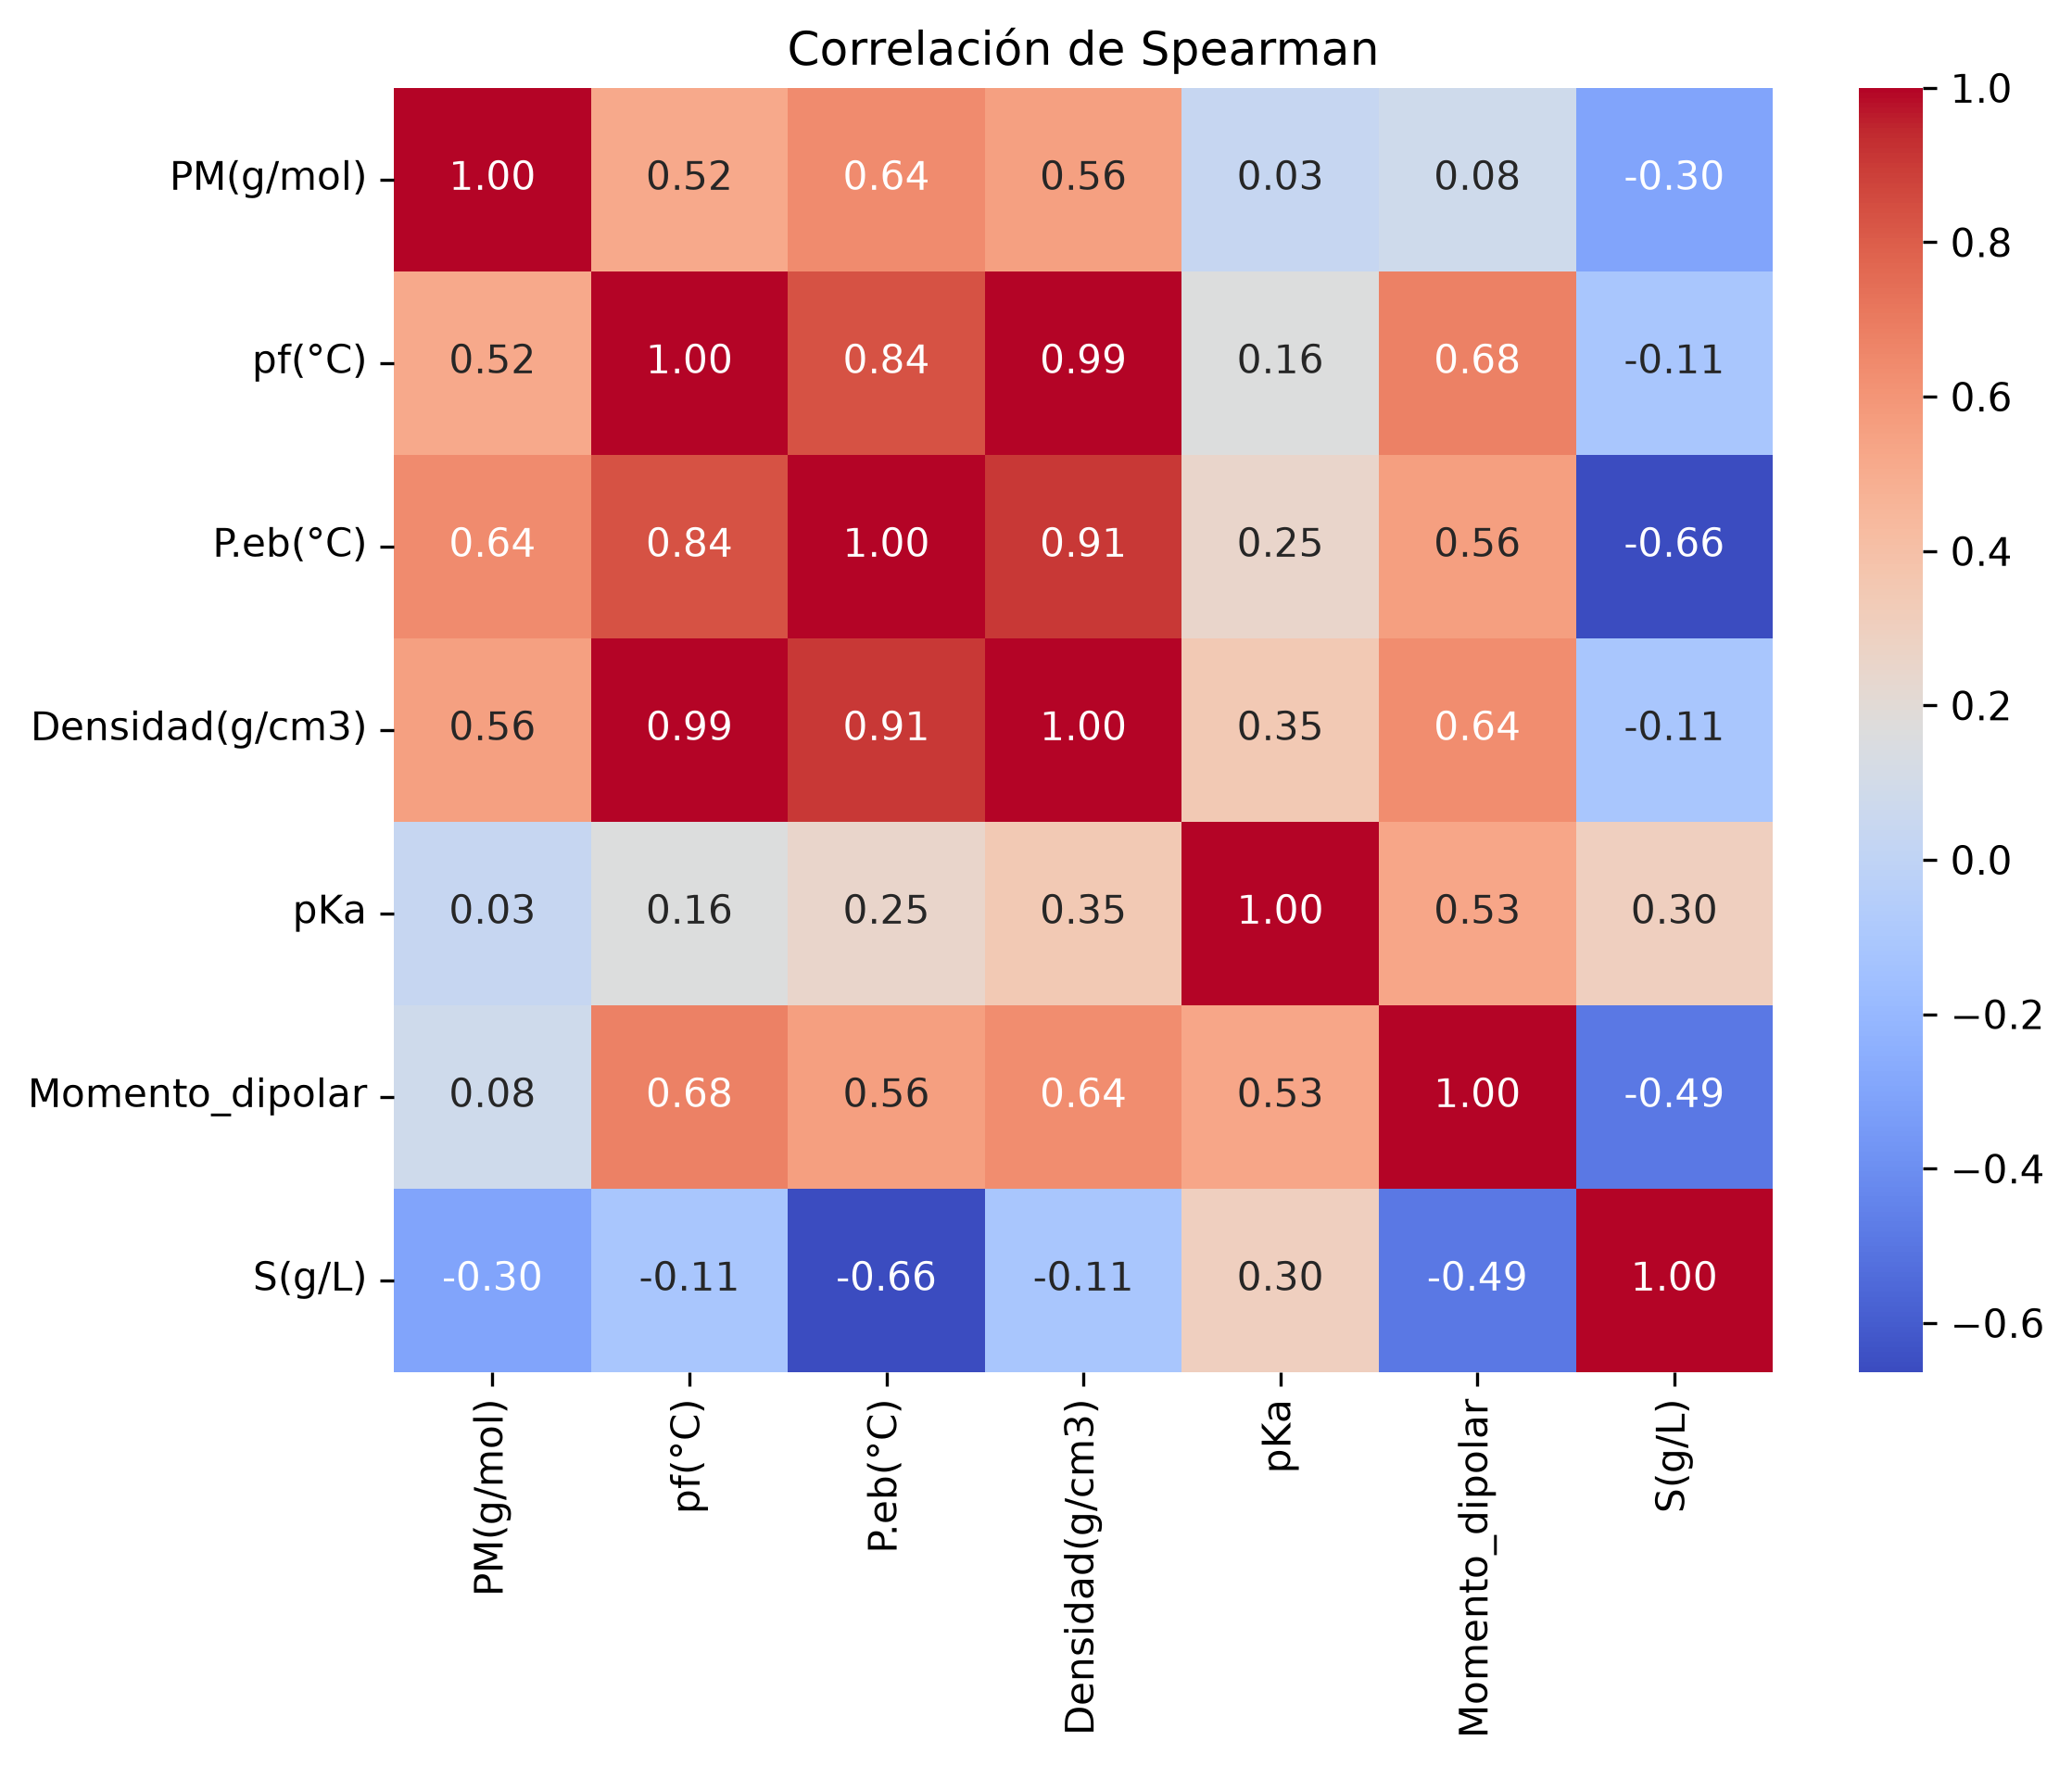
\includegraphics[width=\columnwidth]{01_heatmap_spearman.png}
	\caption{Matriz de correlación de Spearman entre las propiedades fisicoquímicas.}
	\label{fig:heatmap}
\end{figure}

\begin{figure}[htbp]
	\centering
	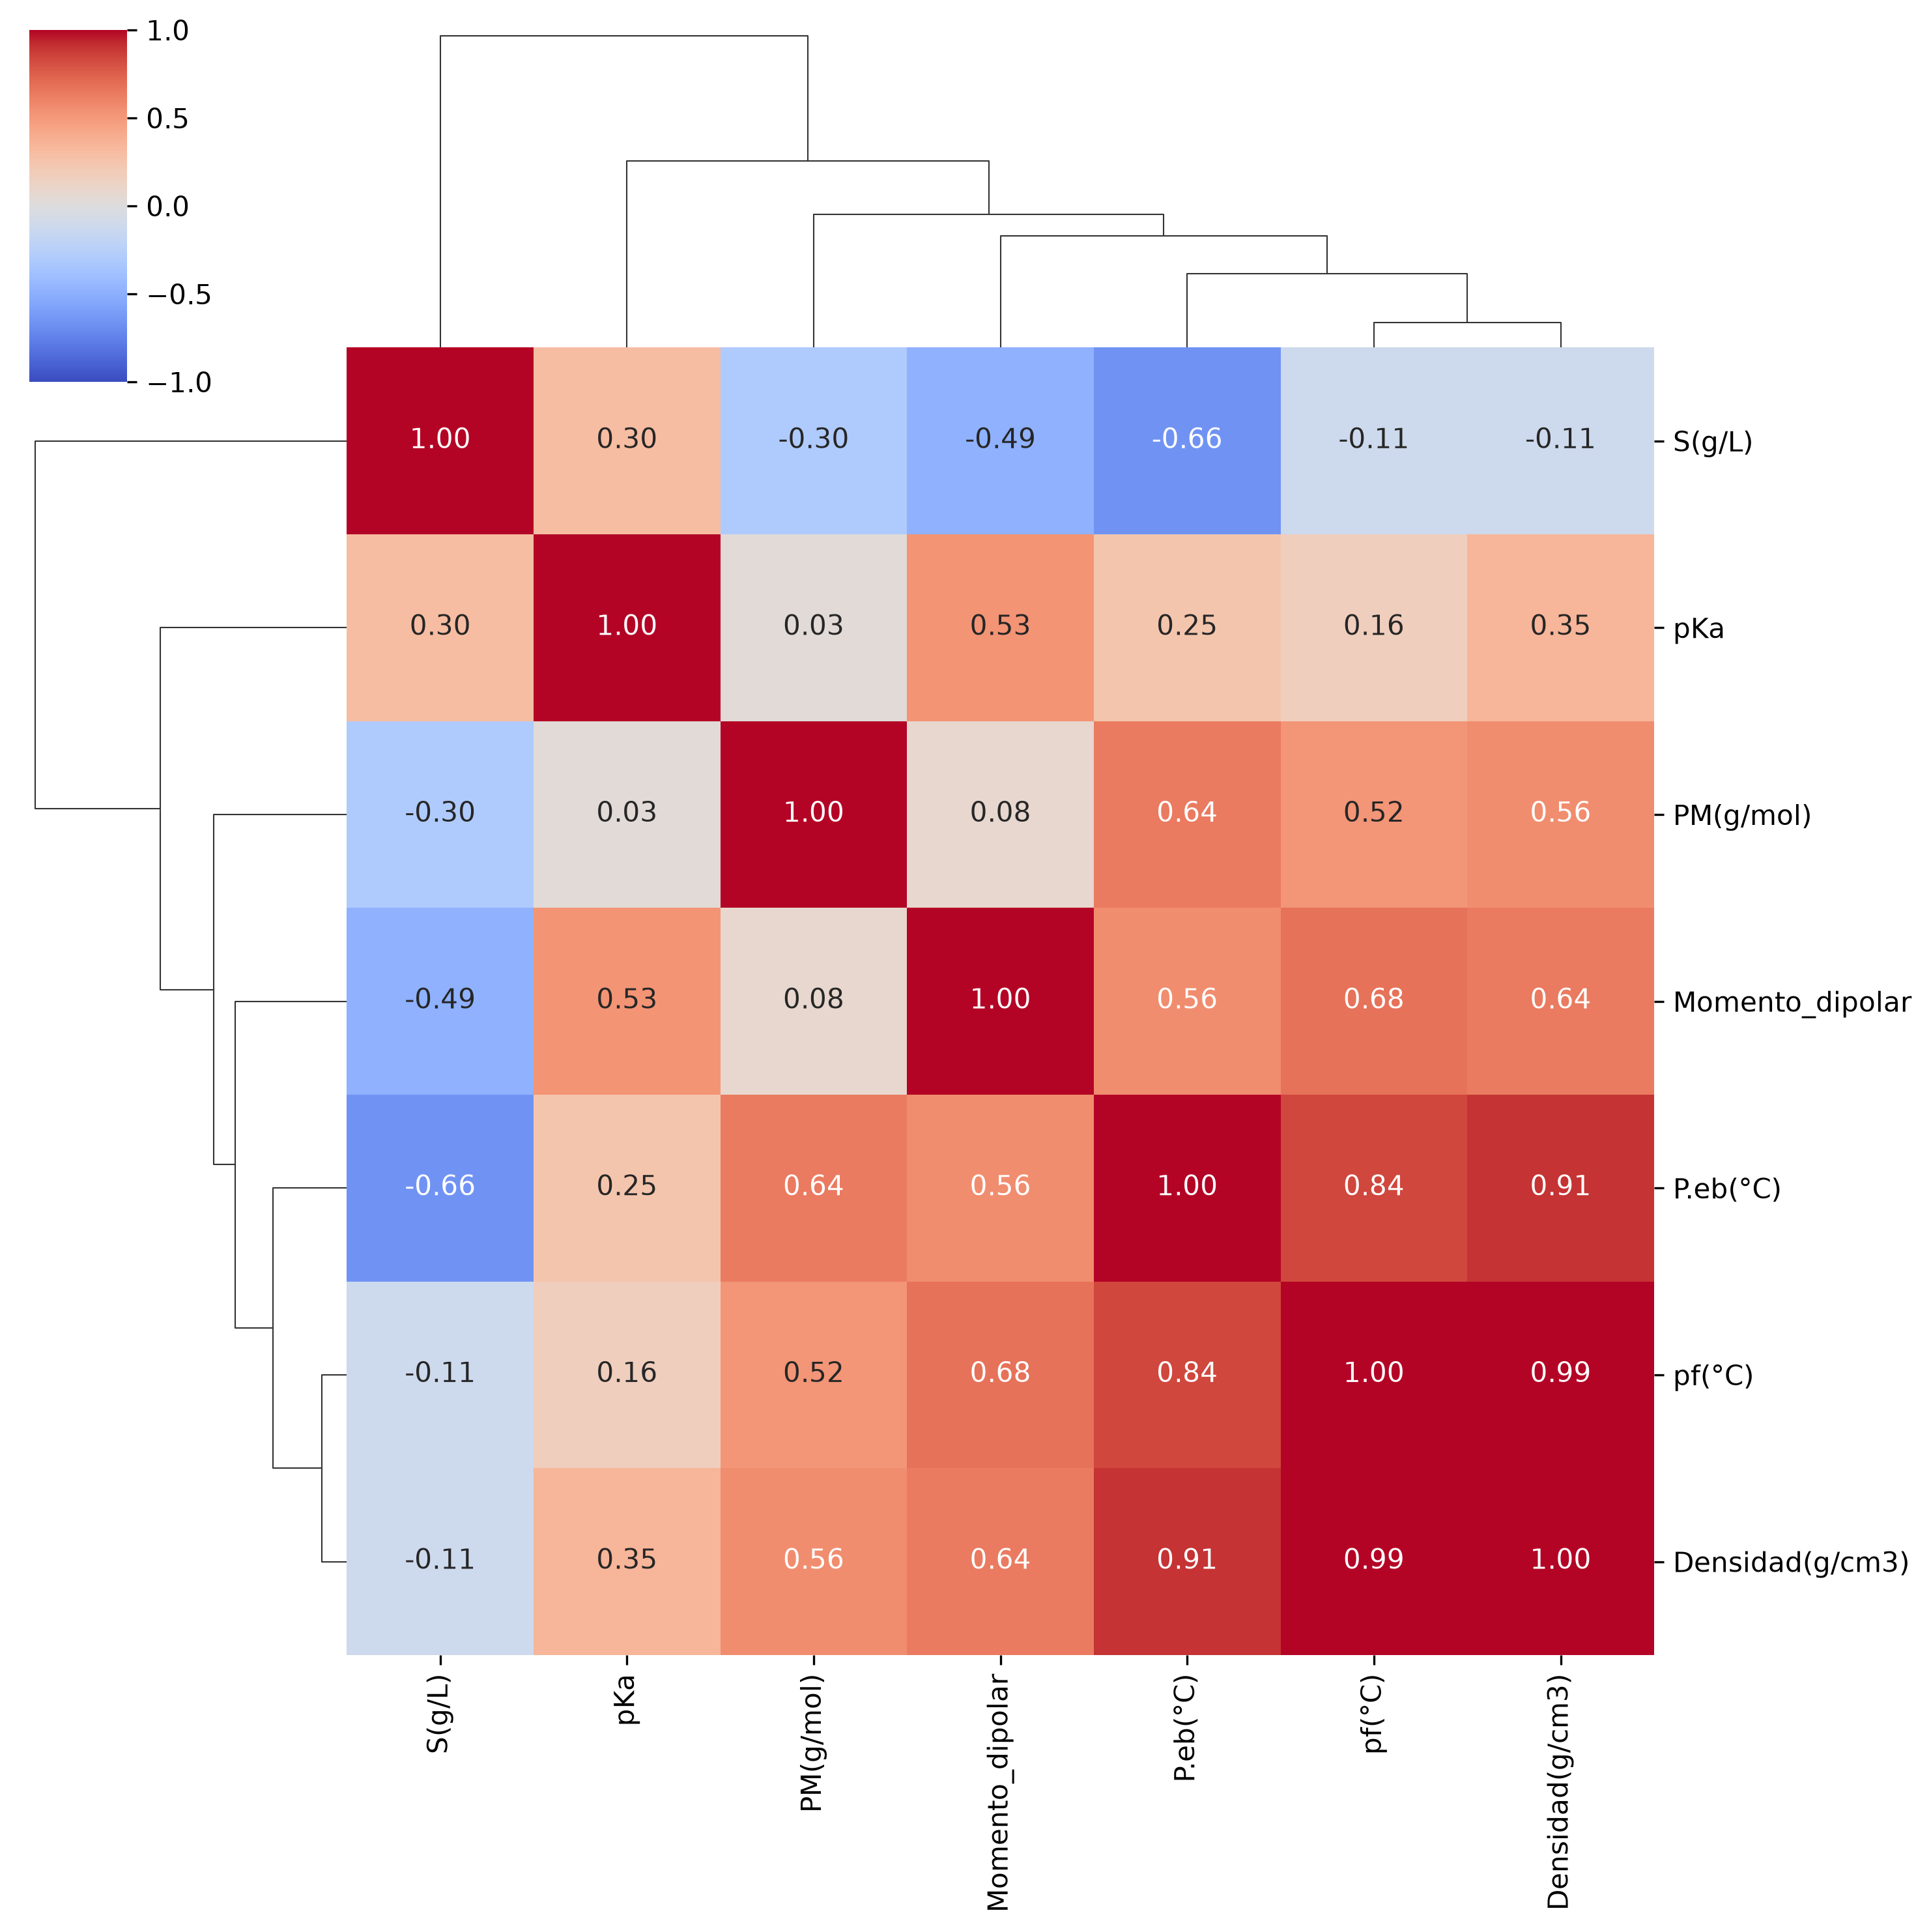
\includegraphics[width=\columnwidth]{02_clustermap_spearman.png}
	\caption{Mapa de agrupamiento jerárquico de la correlación de Spearman.}
	\label{fig:clustermap}
\end{figure}

\subsection{Tendencias entre propiedades}
% TODO (Valentina): discutir cada regresión en términos de fuerzas intermoleculares.
Las Figuras~\ref{fig:pf-dens}--\ref{fig:dip-peb} muestran las regresiones
lineales entre pares de propiedades, con su intervalo de confianza.
\textit{[Interpretación pendiente.]}

\begin{figure}[htbp]
	\centering
	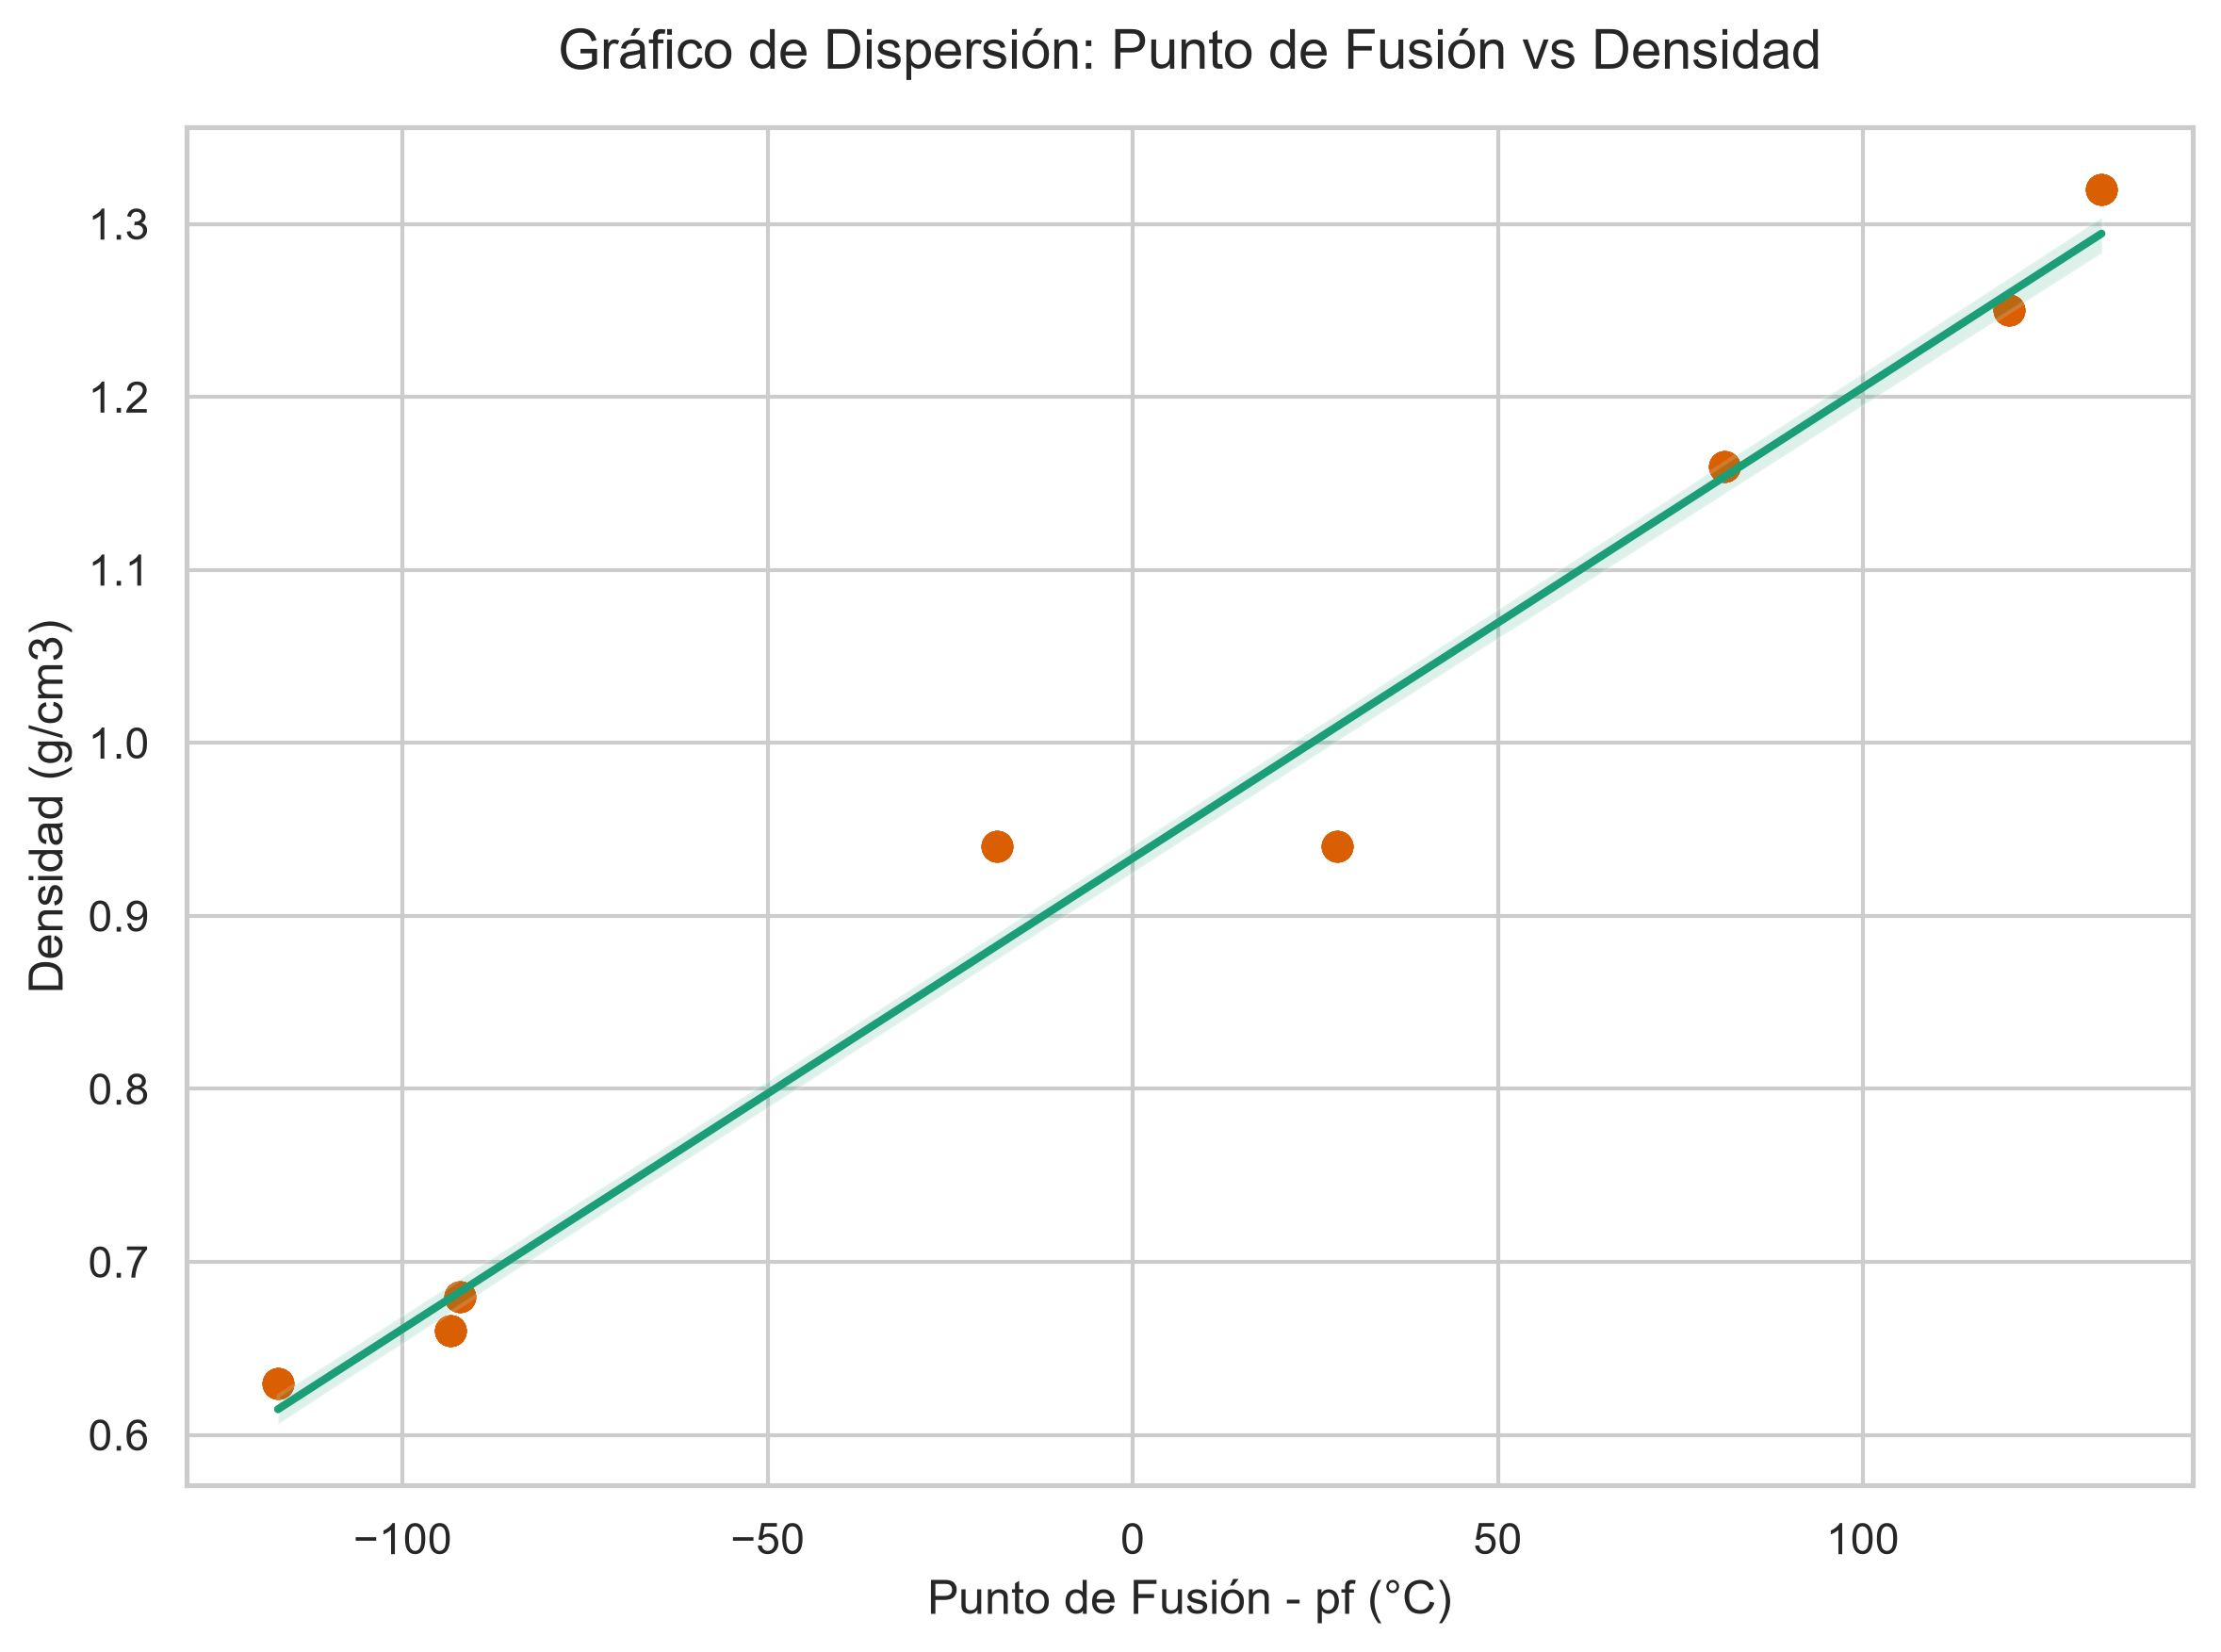
\includegraphics[width=\columnwidth]{03_reg_pf_vs_densidad.png}
	\caption{Punto de fusión frente a densidad.}
	\label{fig:pf-dens}
\end{figure}

\begin{figure}[htbp]
	\centering
	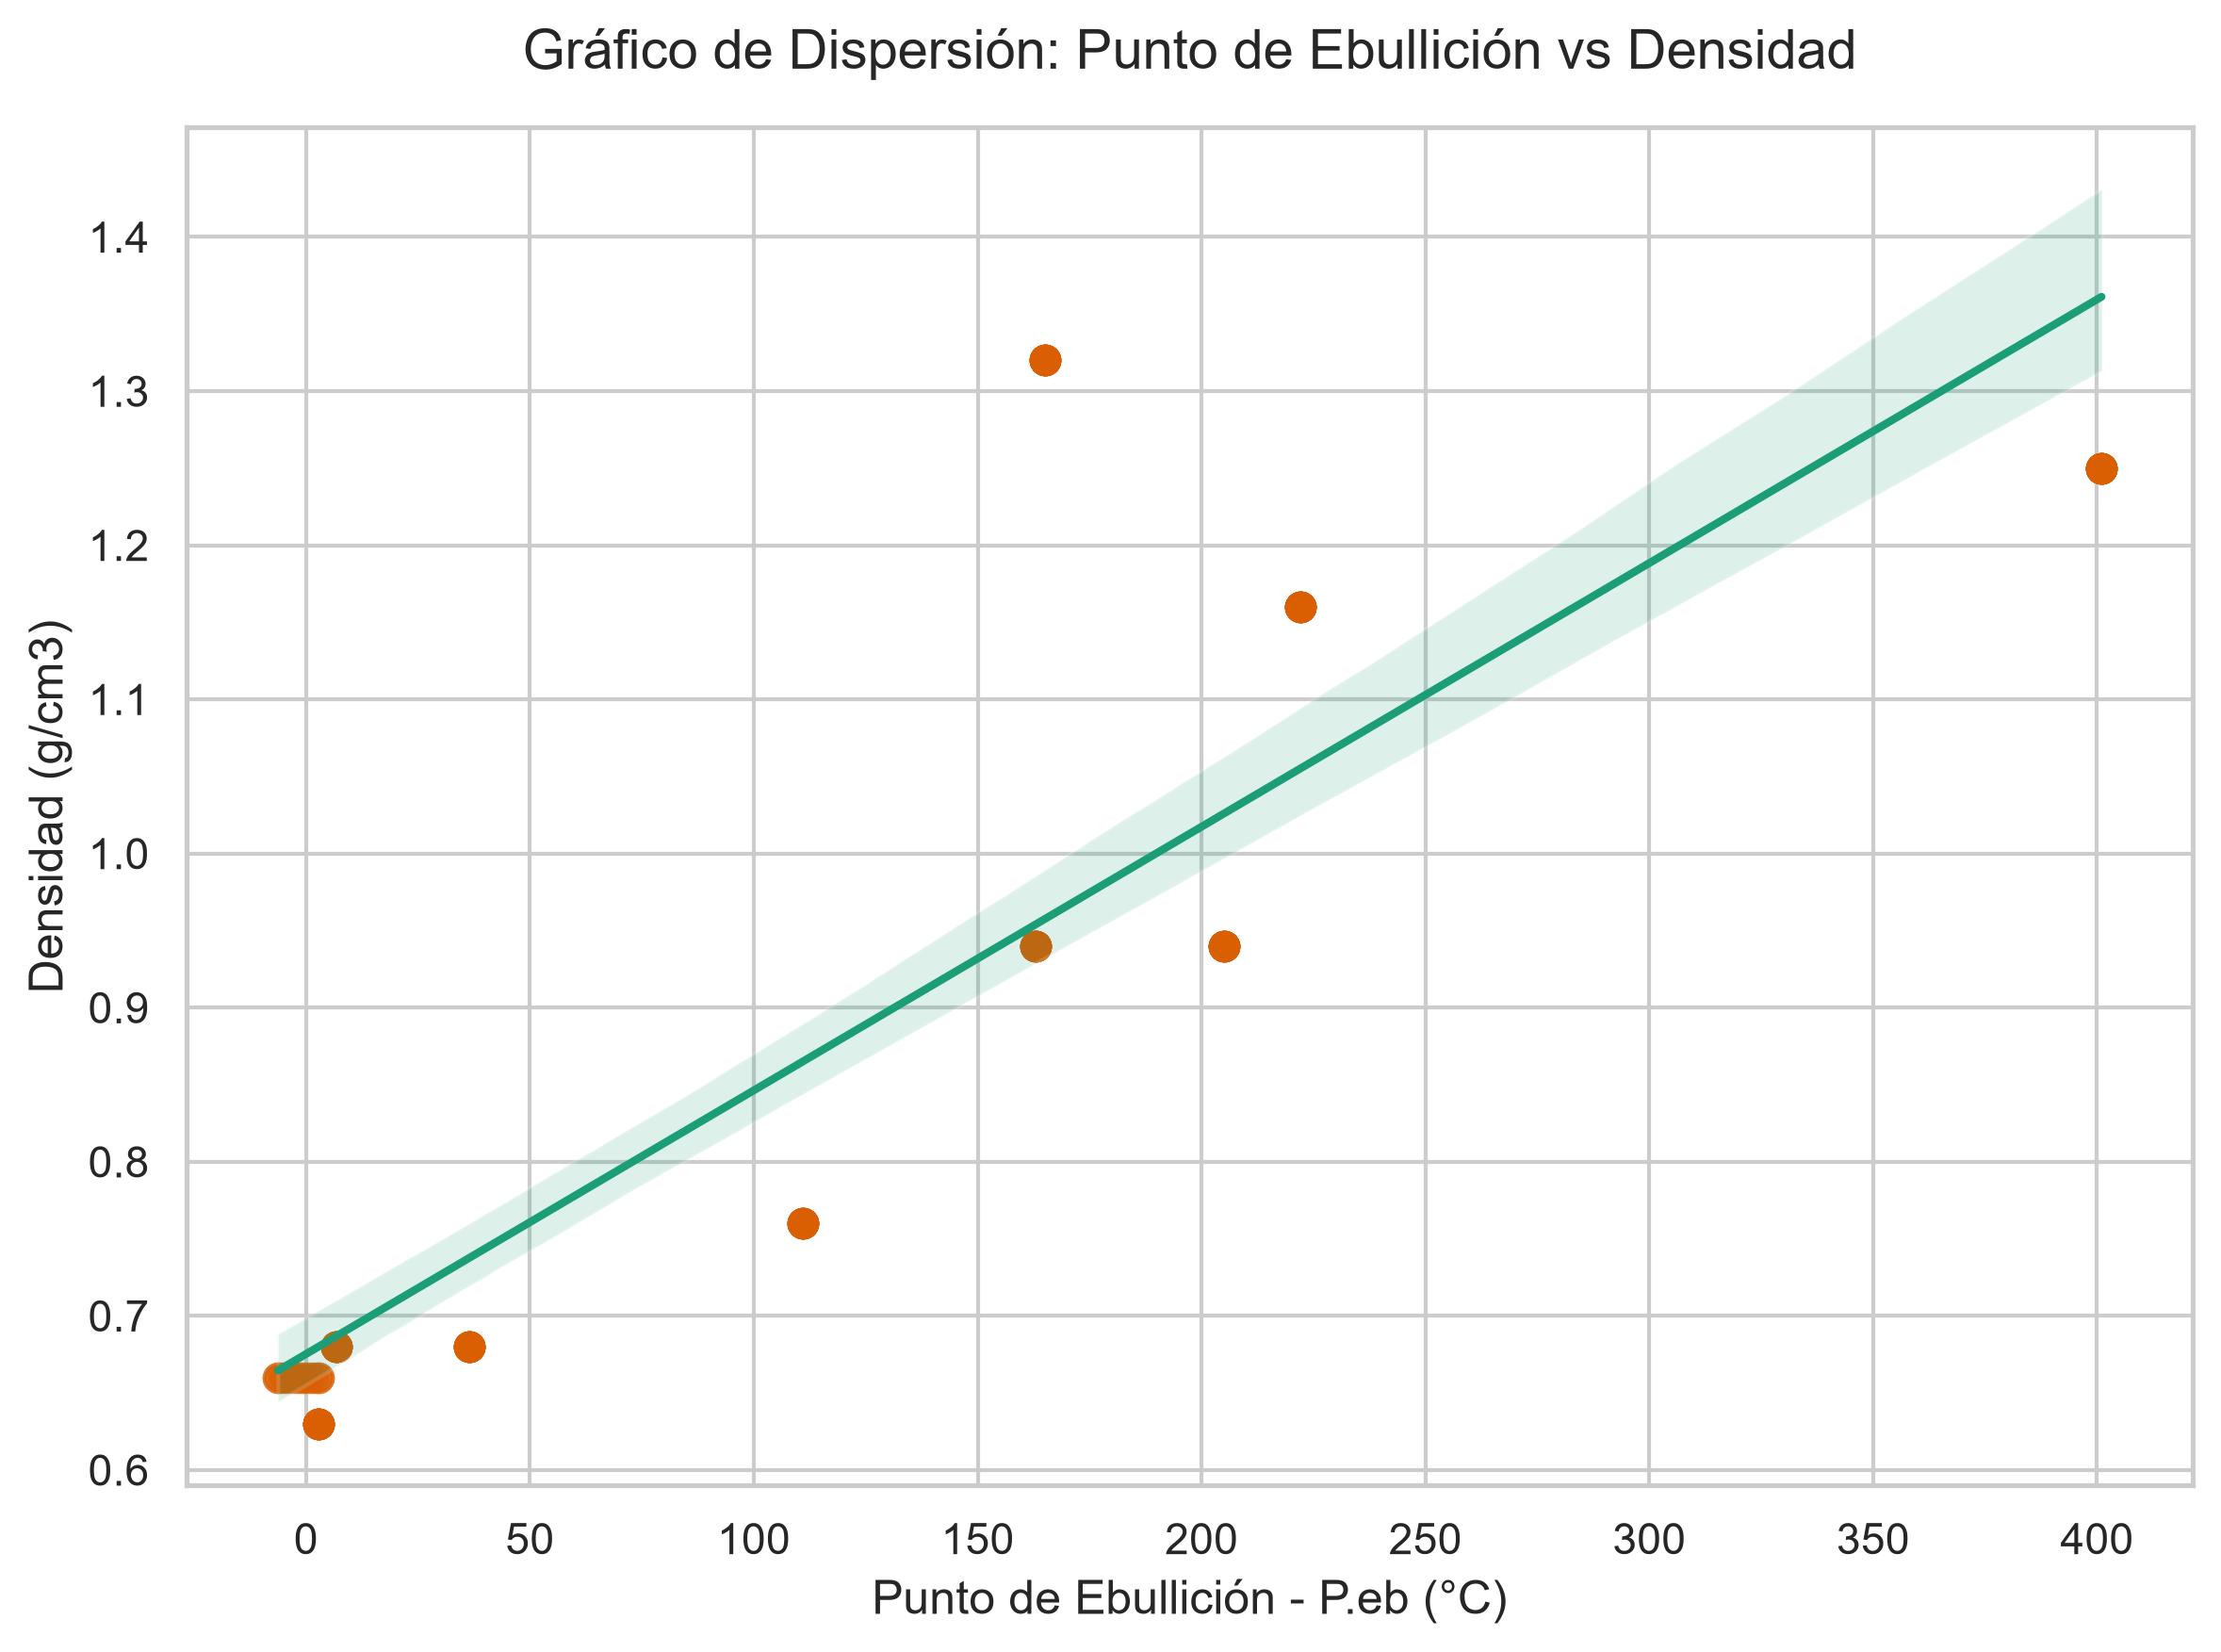
\includegraphics[width=\columnwidth]{04_reg_peb_vs_densidad.png}
	\caption{Punto de ebullición frente a densidad.}
	\label{fig:peb-dens}
\end{figure}

\begin{figure}[htbp]
	\centering
	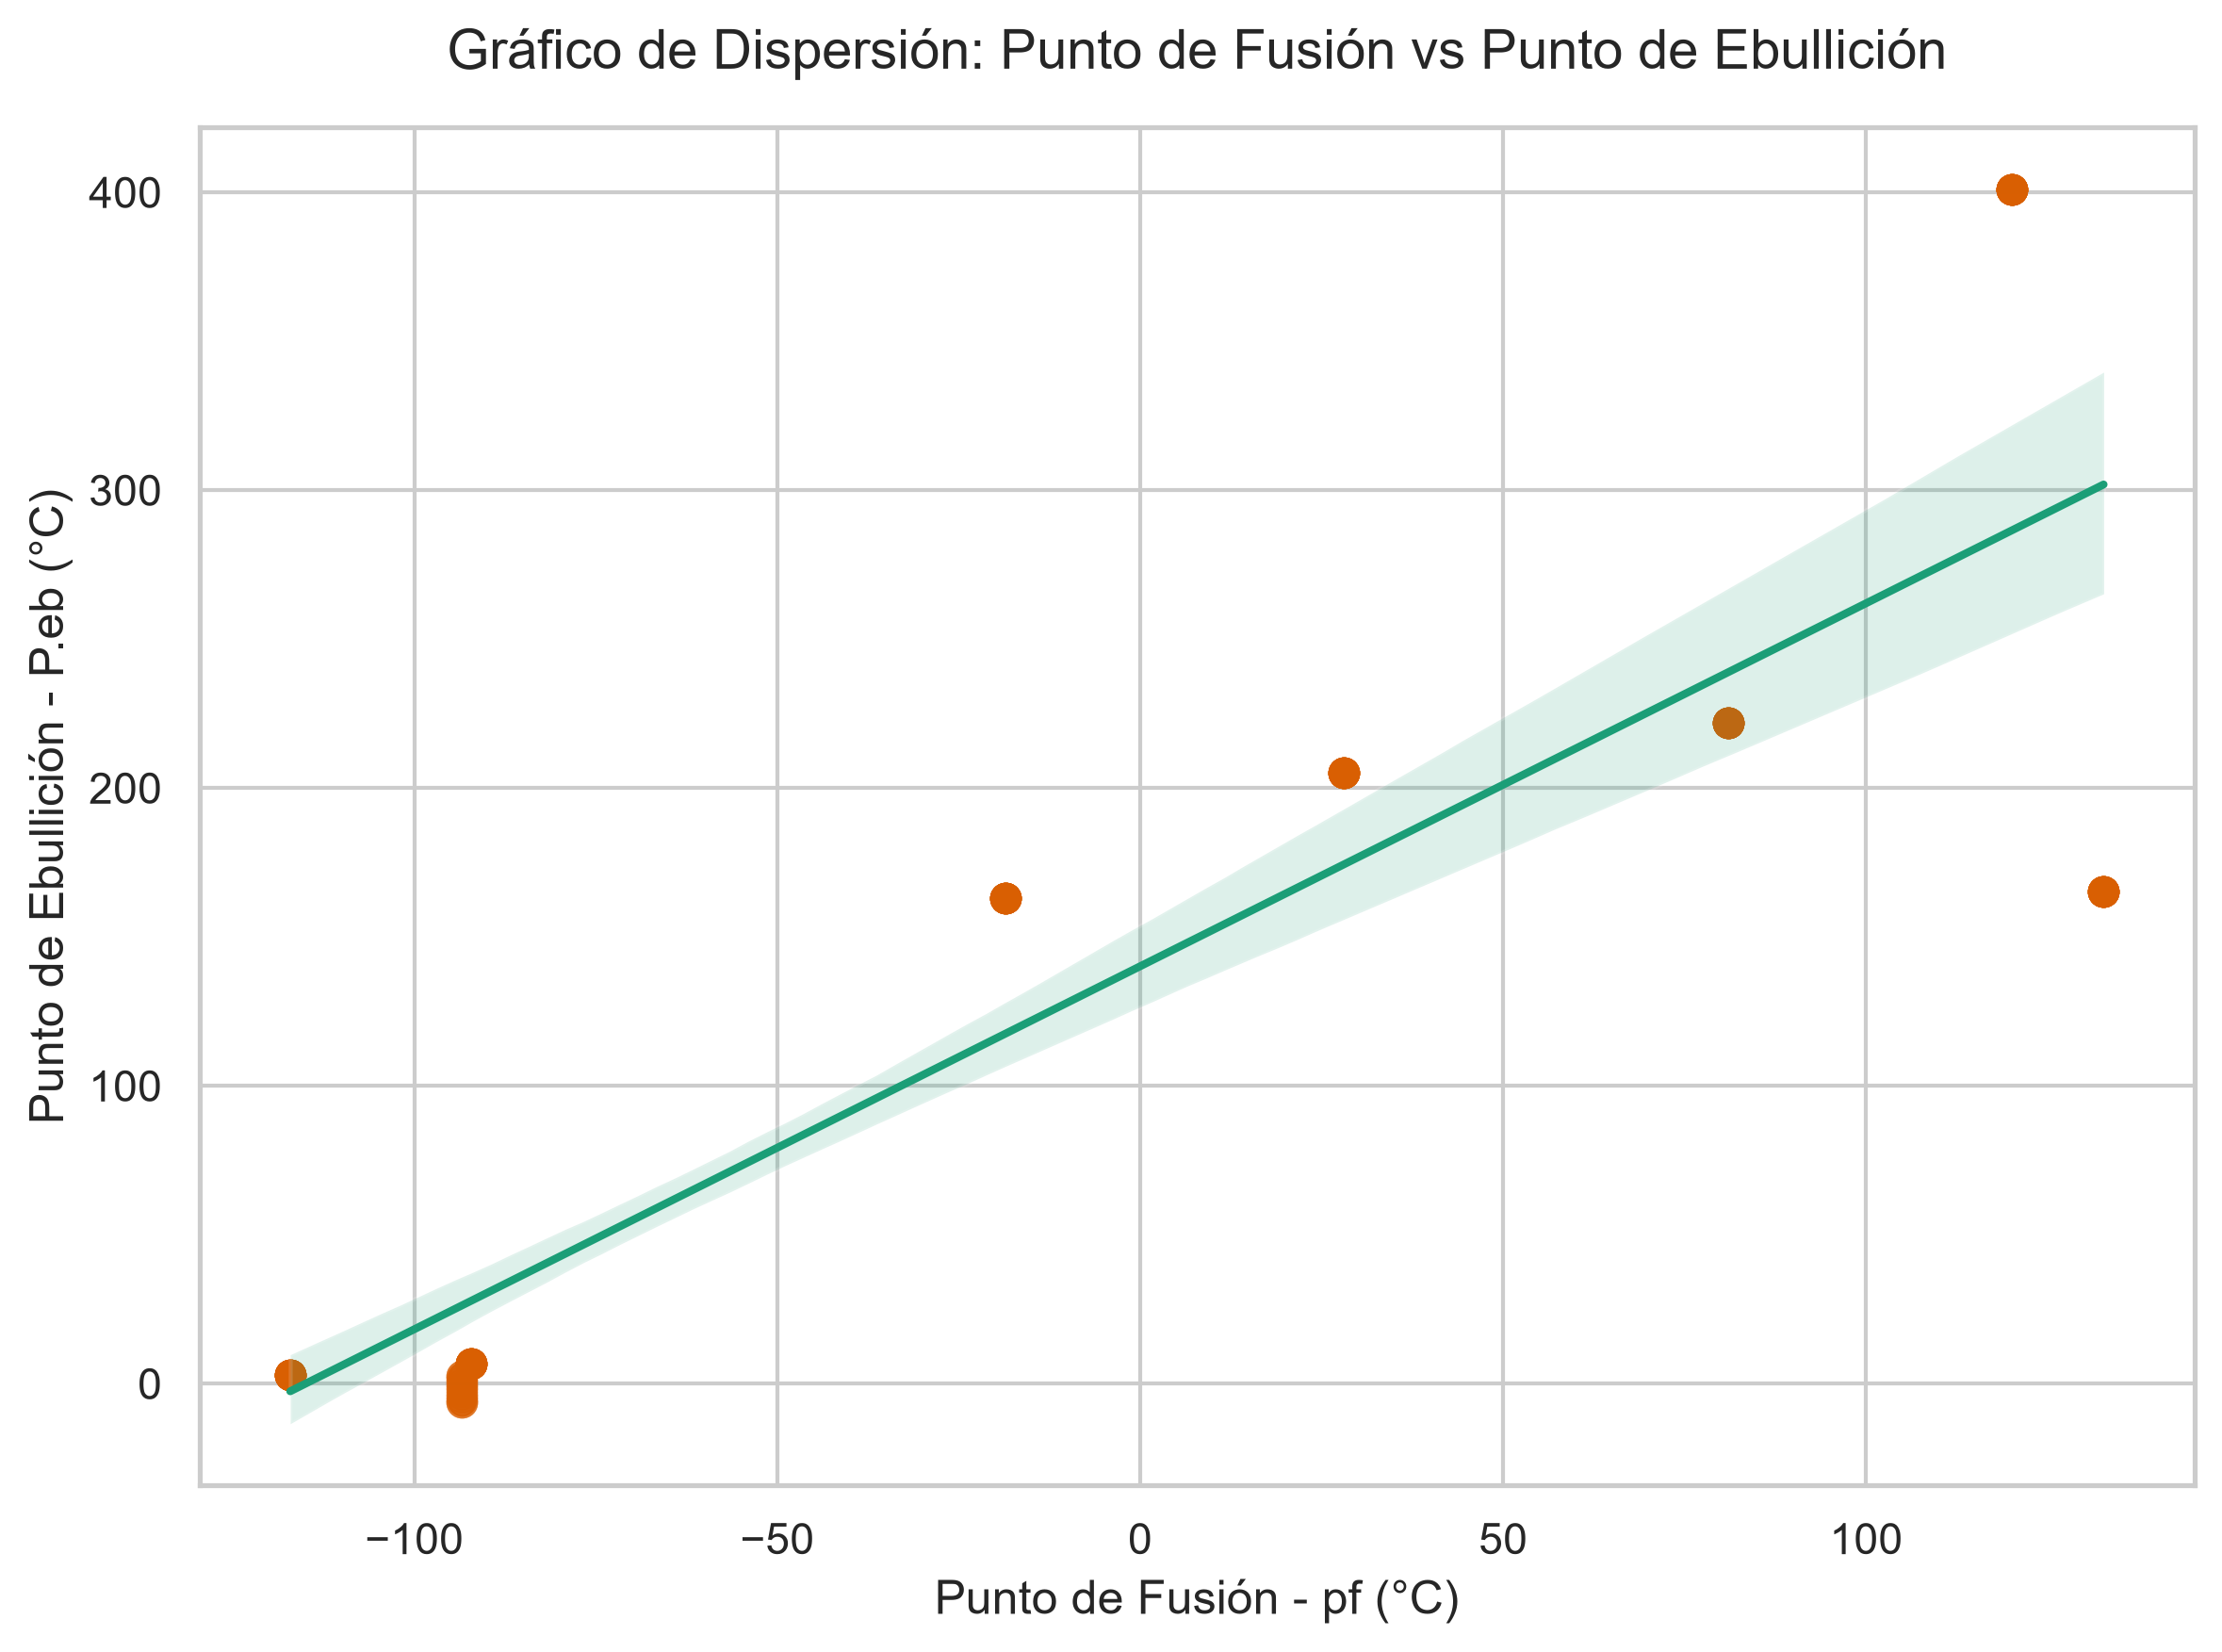
\includegraphics[width=\columnwidth]{05_reg_pf_vs_peb.png}
	\caption{Punto de fusión frente a punto de ebullición.}
	\label{fig:pf-peb}
\end{figure}

\begin{figure}[htbp]
	\centering
	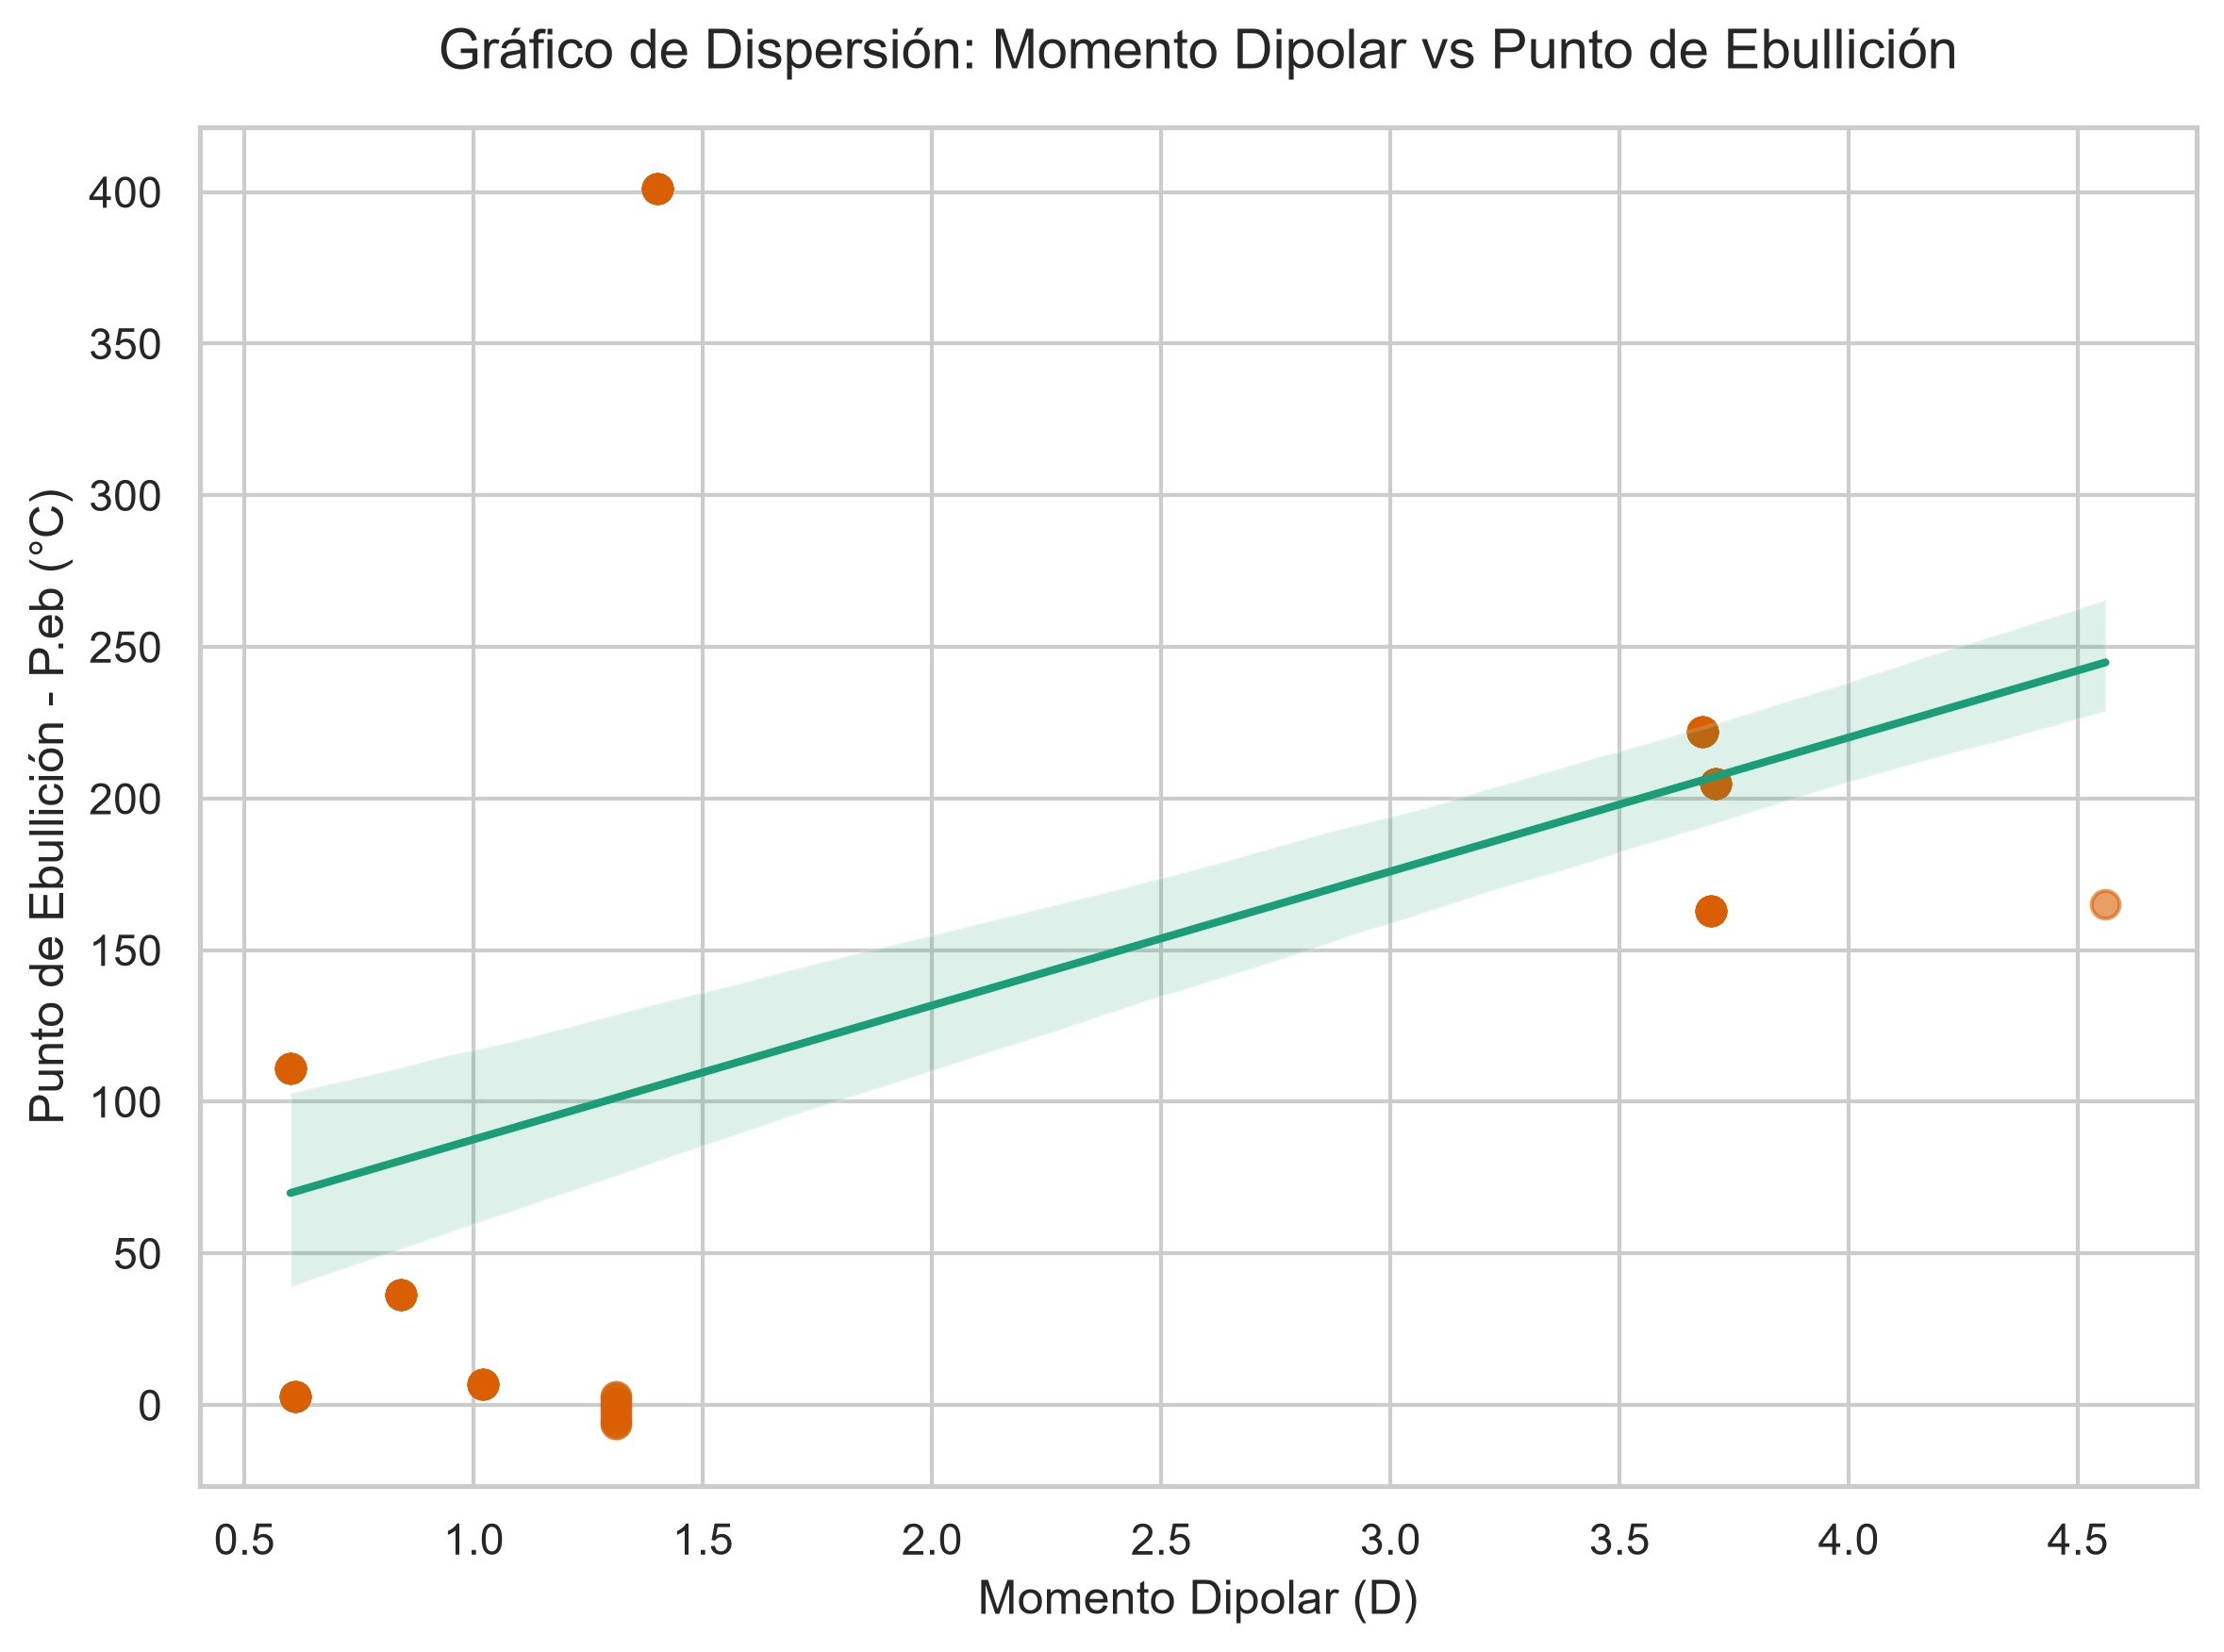
\includegraphics[width=\columnwidth]{06_reg_dipolo_vs_peb.png}
	\caption{Momento dipolar frente a punto de ebullición.}
	\label{fig:dip-peb}
\end{figure}

\subsection{Exploración interactiva con Plotly}
% TODO (Valentina): interpretar; idea central: a igual PM, los compuestos con
% enlace N--H (donadores de puente de H) hierven mucho más alto.
Las Figuras~\ref{fig:burbujas}--\ref{fig:dens-sol} se generaron con Plotly,
una fila por compuesto; sus versiones HTML permiten inspeccionar cada molécula
con el cursor. En la Figura~\ref{fig:burbujas}, trimetilamina
(\SI{2.8}{\degreeCelsius}) y N-metiletanamina (\SI{36.5}{\degreeCelsius}) tienen
el mismo peso molecular (\SI{59.11}{\gram\per\mole}): la diferencia se debe a que
sólo la segunda posee enlace N--H y forma puentes de hidrógeno.
\textit{[Interpretación pendiente.]}

\begin{figure}[htbp]
	\centering
	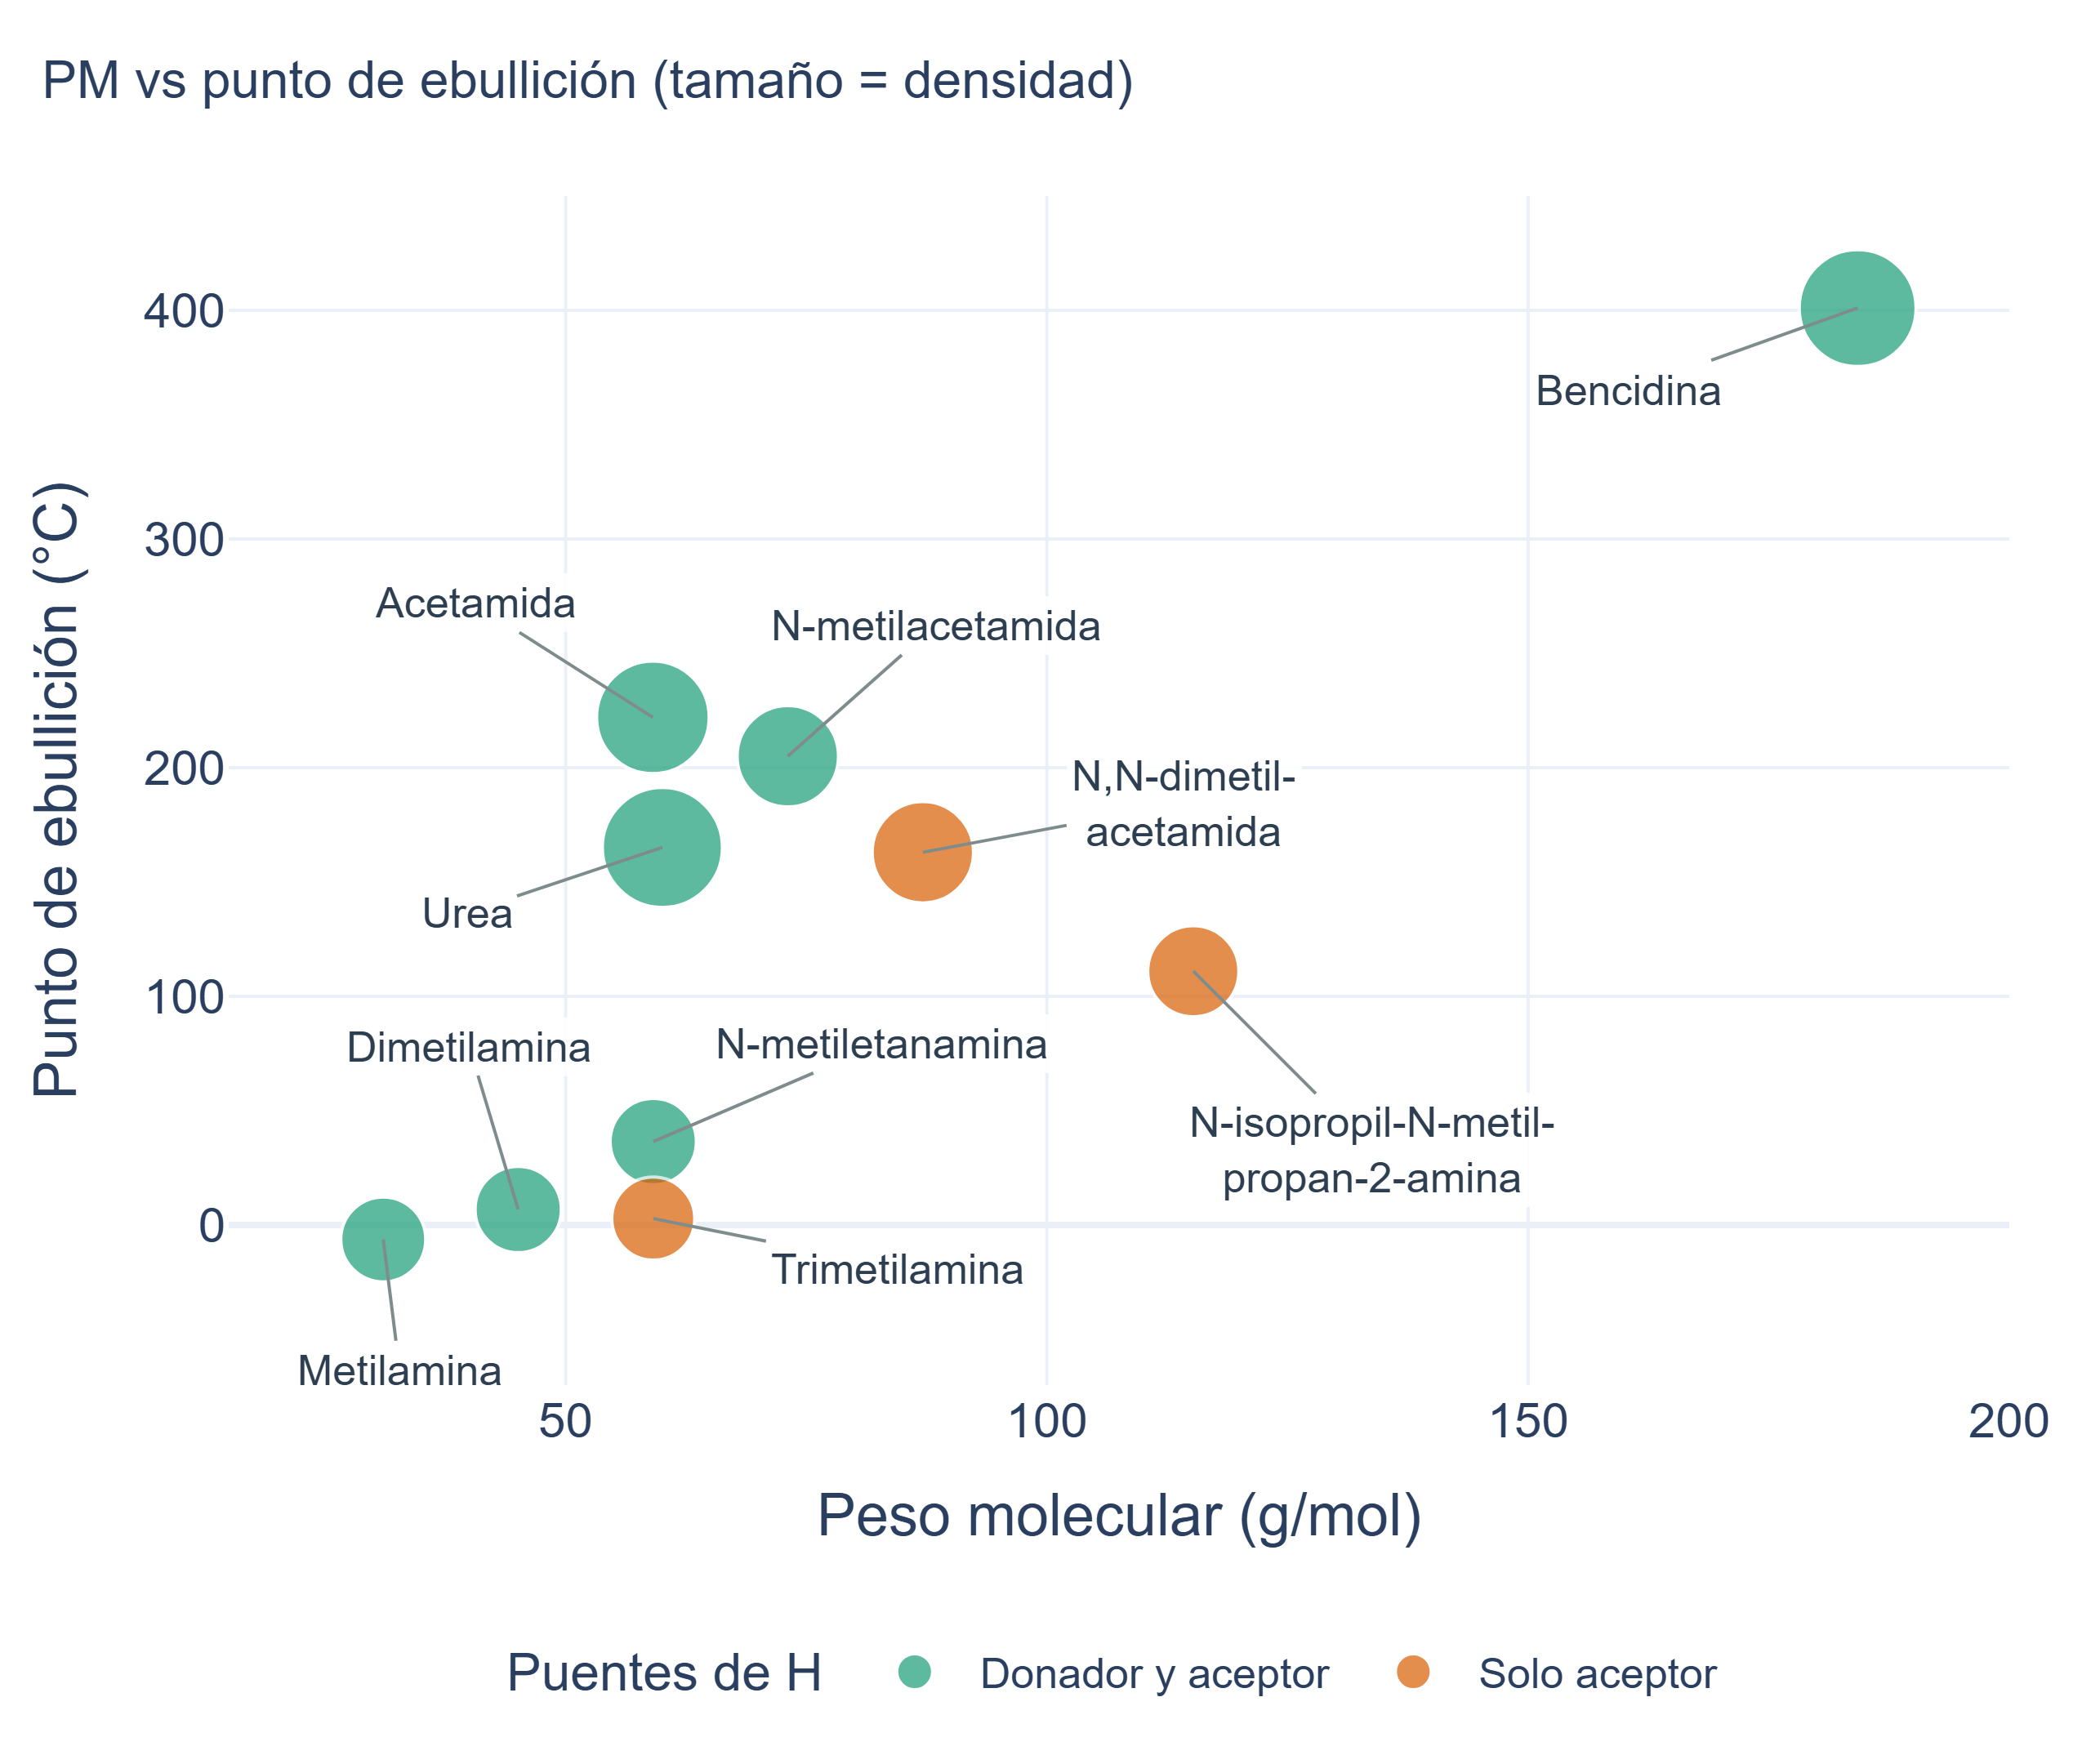
\includegraphics[width=\columnwidth]{11_plotly_burbujas_pm_peb.png}
	\caption{Peso molecular frente a punto de ebullición; el tamaño representa la densidad y el color la capacidad de formar puentes de hidrógeno.}
	\label{fig:burbujas}
\end{figure}

\begin{figure}[htbp]
	\centering
	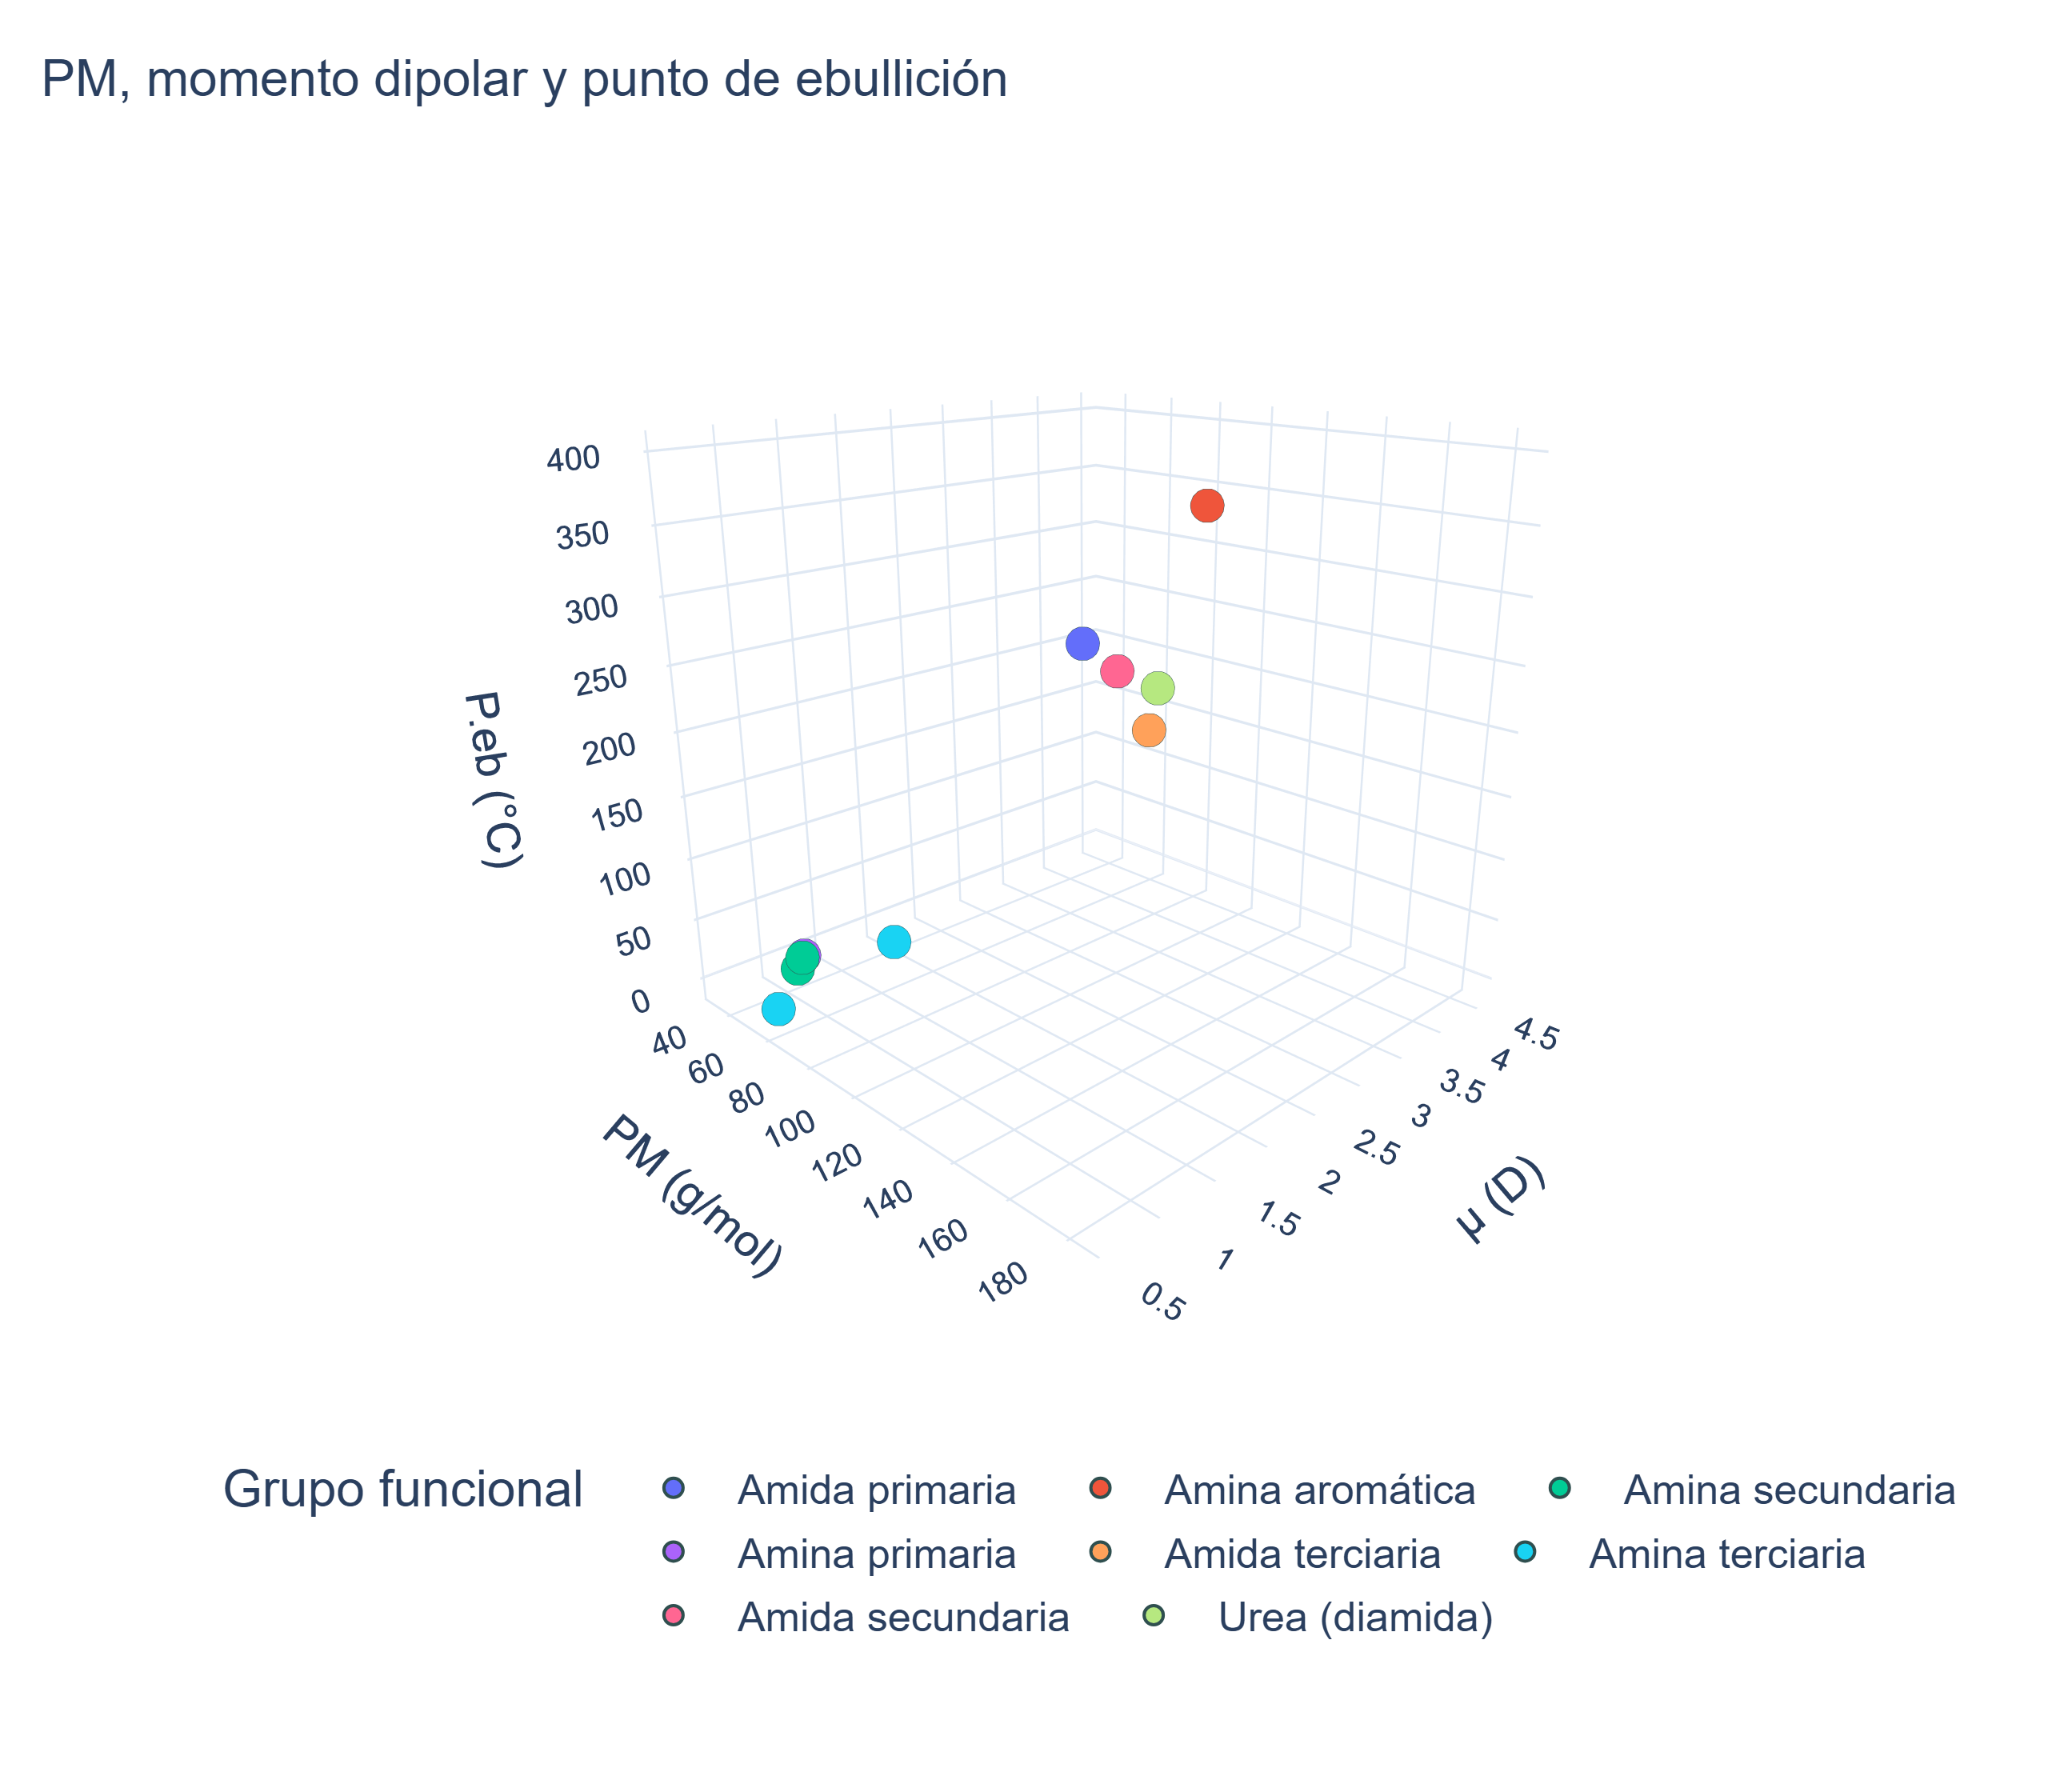
\includegraphics[width=\columnwidth]{12_plotly_3d_pm_dipolo_peb.png}
	\caption{Espacio tridimensional de peso molecular, momento dipolar y punto de ebullición por grupo funcional.}
	\label{fig:3d}
\end{figure}

\begin{figure}[htbp]
	\centering
	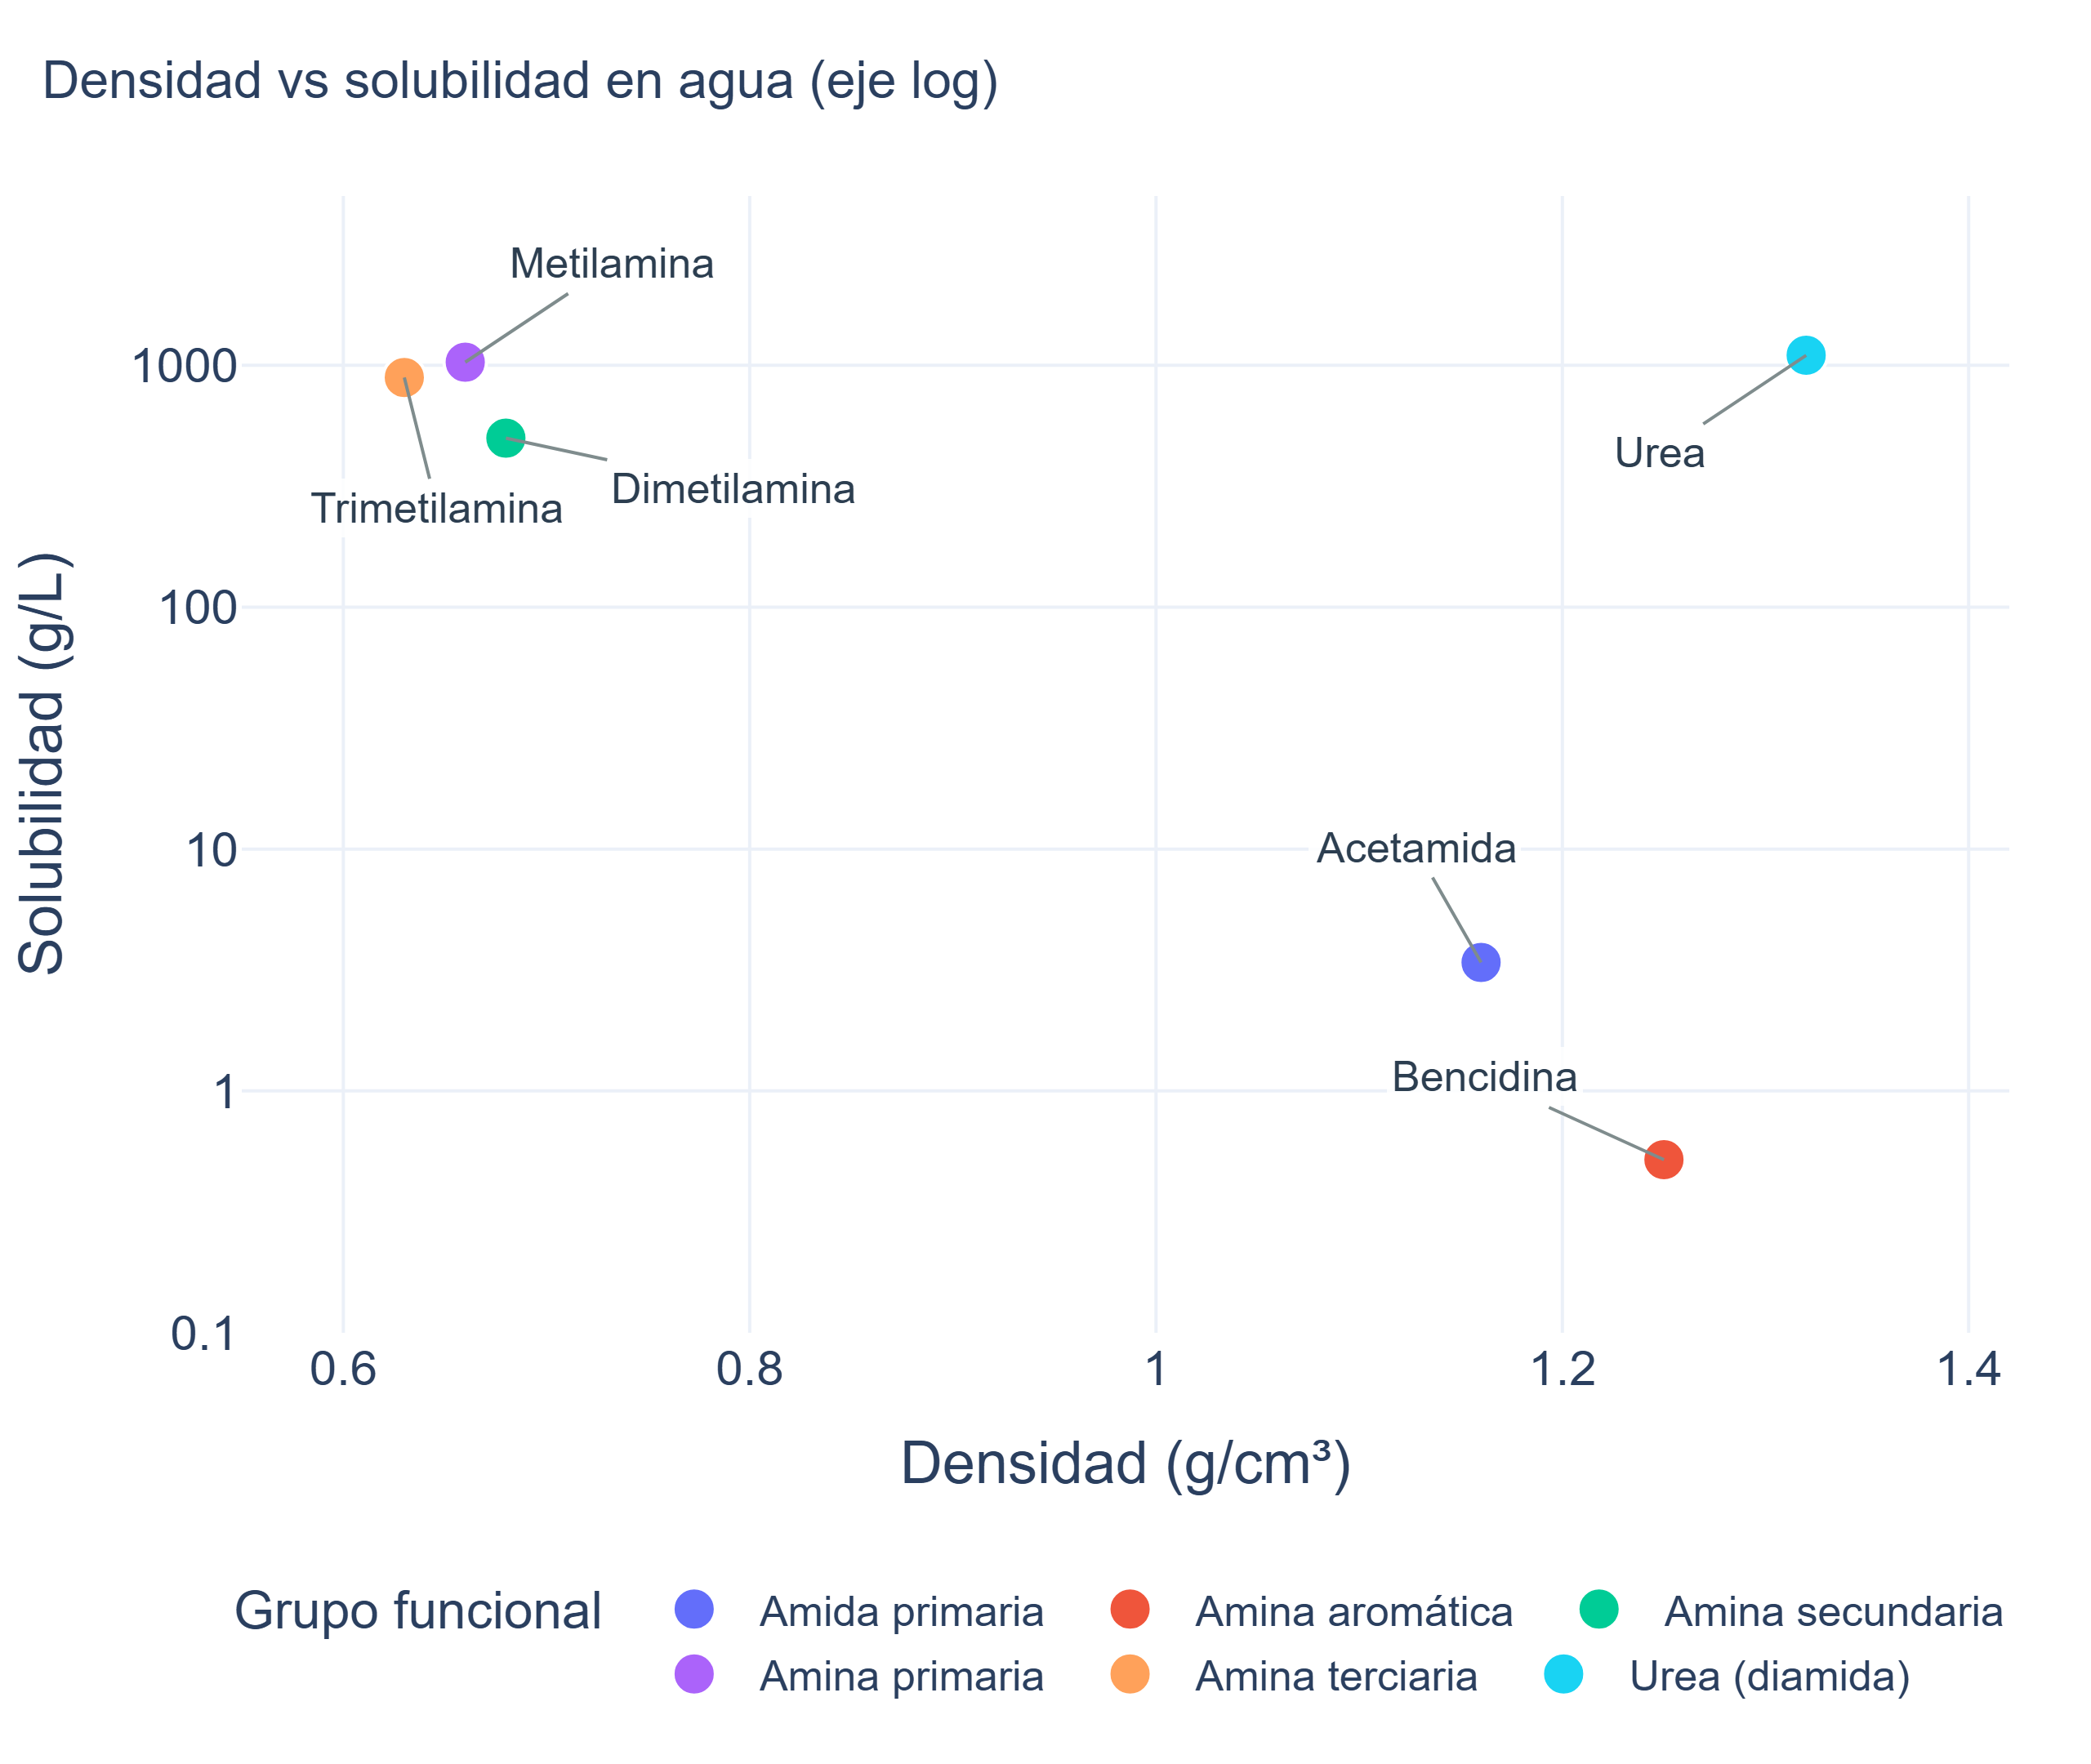
\includegraphics[width=\columnwidth]{13_plotly_densidad_solubilidad.png}
	\caption{Densidad frente a solubilidad en agua (eje logarítmico).}
	\label{fig:dens-sol}
\end{figure}

\subsection{Distribución por tipo de reacción y medio}
% TODO (Valentina): explicar qué representa TR y comparar medianas/dispersiones.
La Figura~\ref{fig:frecuencias} compara la frecuencia de cada mecanismo de
reacción y de cada medio; la sustitución nucleofílica (SN) domina, coherente con
el carácter nucleófilo del par libre del nitrógeno. Las
Figuras~\ref{fig:violin}--\ref{fig:dona} describen la distribución de
probabilidad de TR según el tipo de reacción y el medio.
\textit{[Interpretación pendiente.]}

\begin{figure}[htbp]
	\centering
	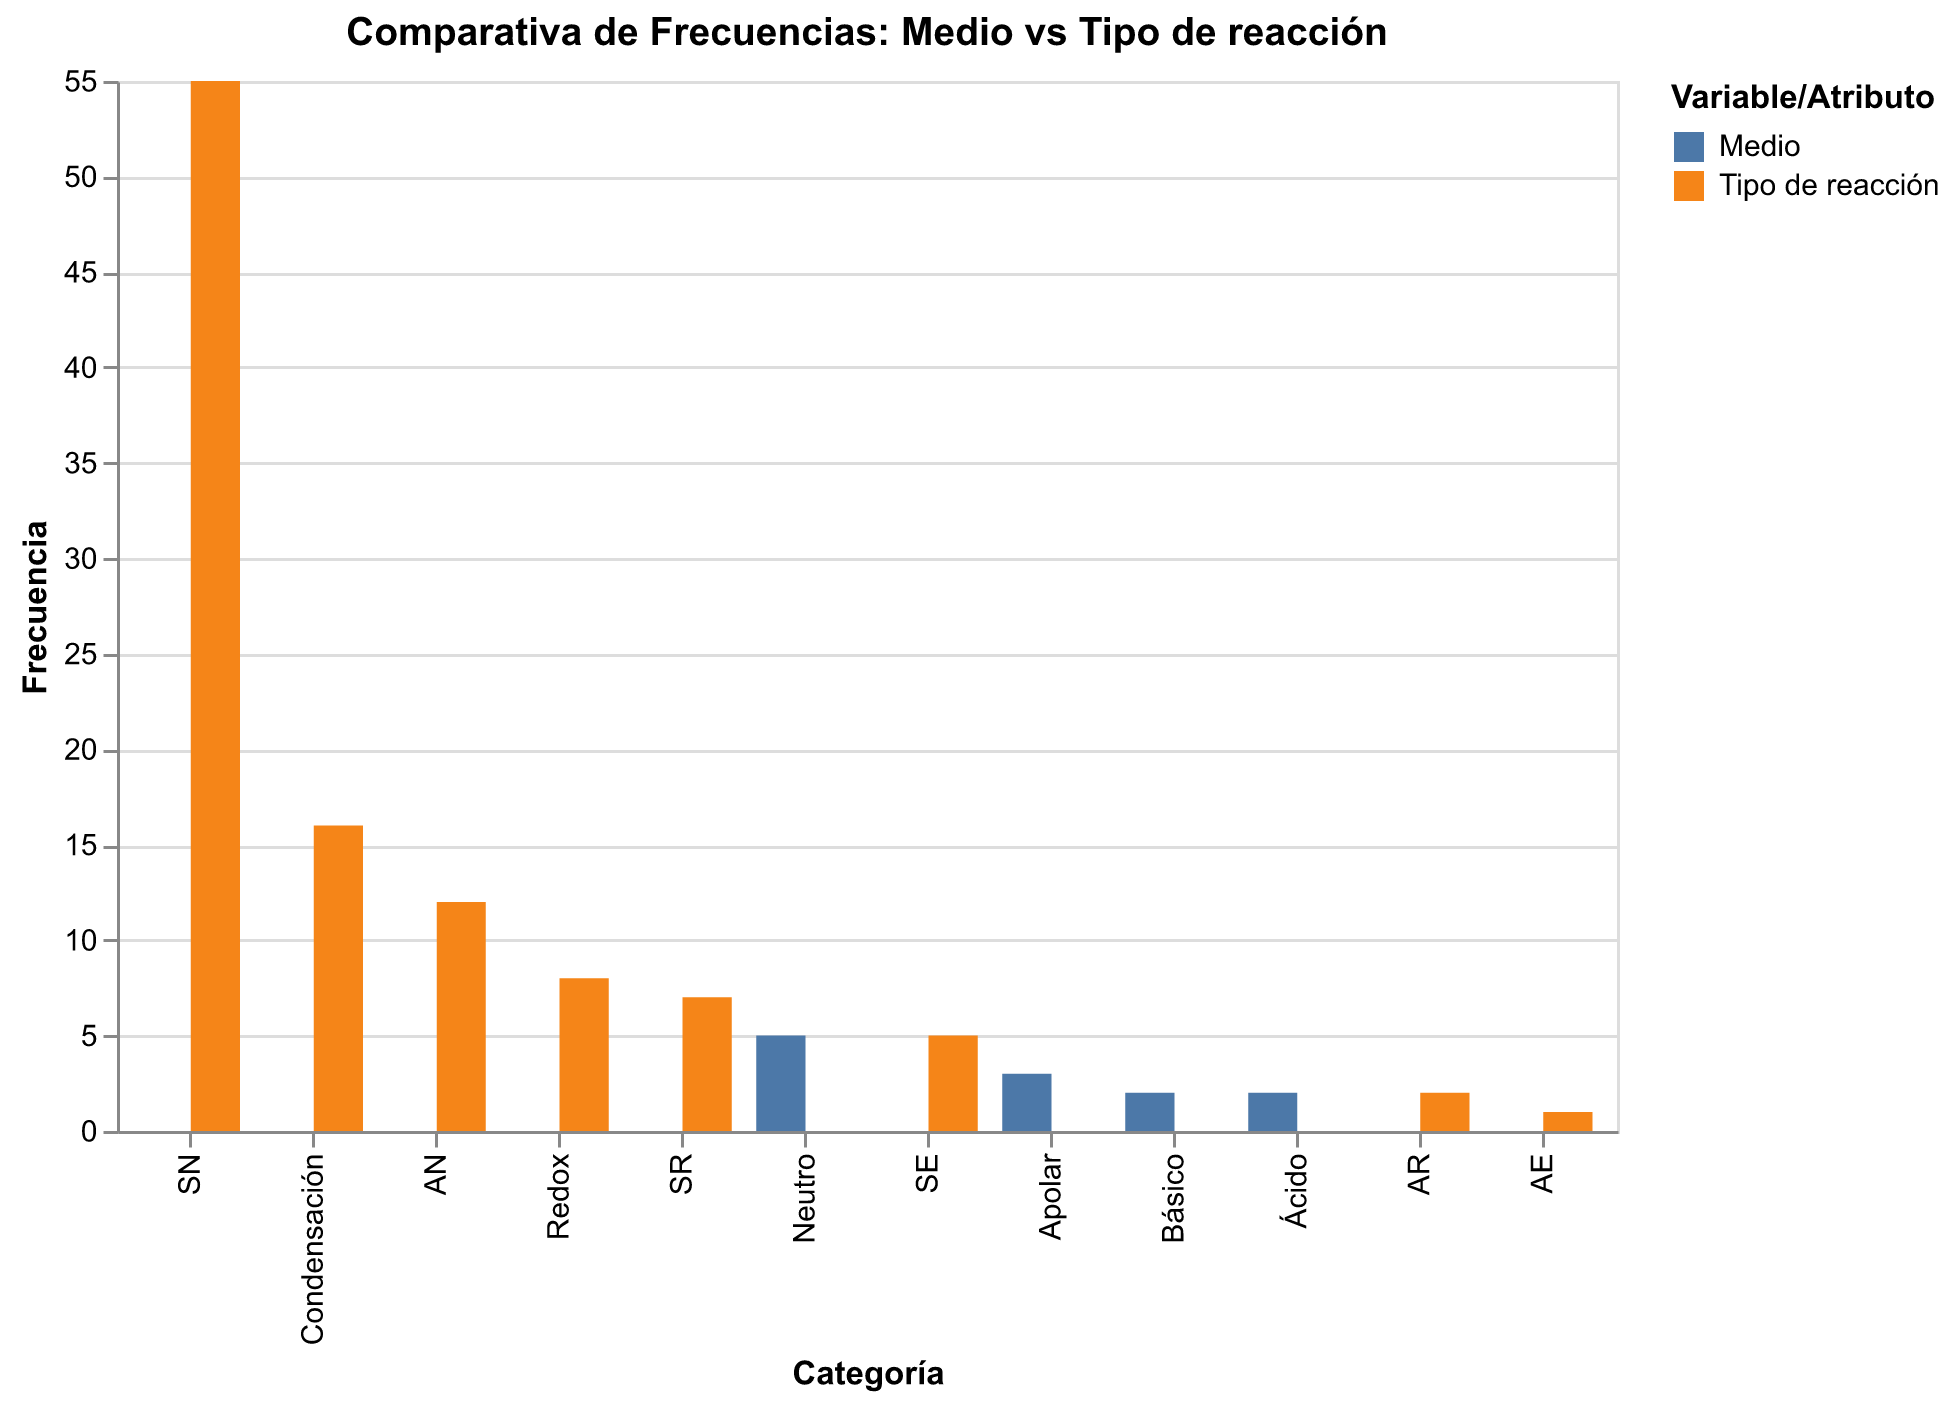
\includegraphics[width=\columnwidth]{09_frecuencias_medio_tipo.png}
	\caption{Frecuencia de los tipos de reacción y de los medios reportados.}
	\label{fig:frecuencias}
\end{figure}

\begin{figure}[htbp]
	\centering
	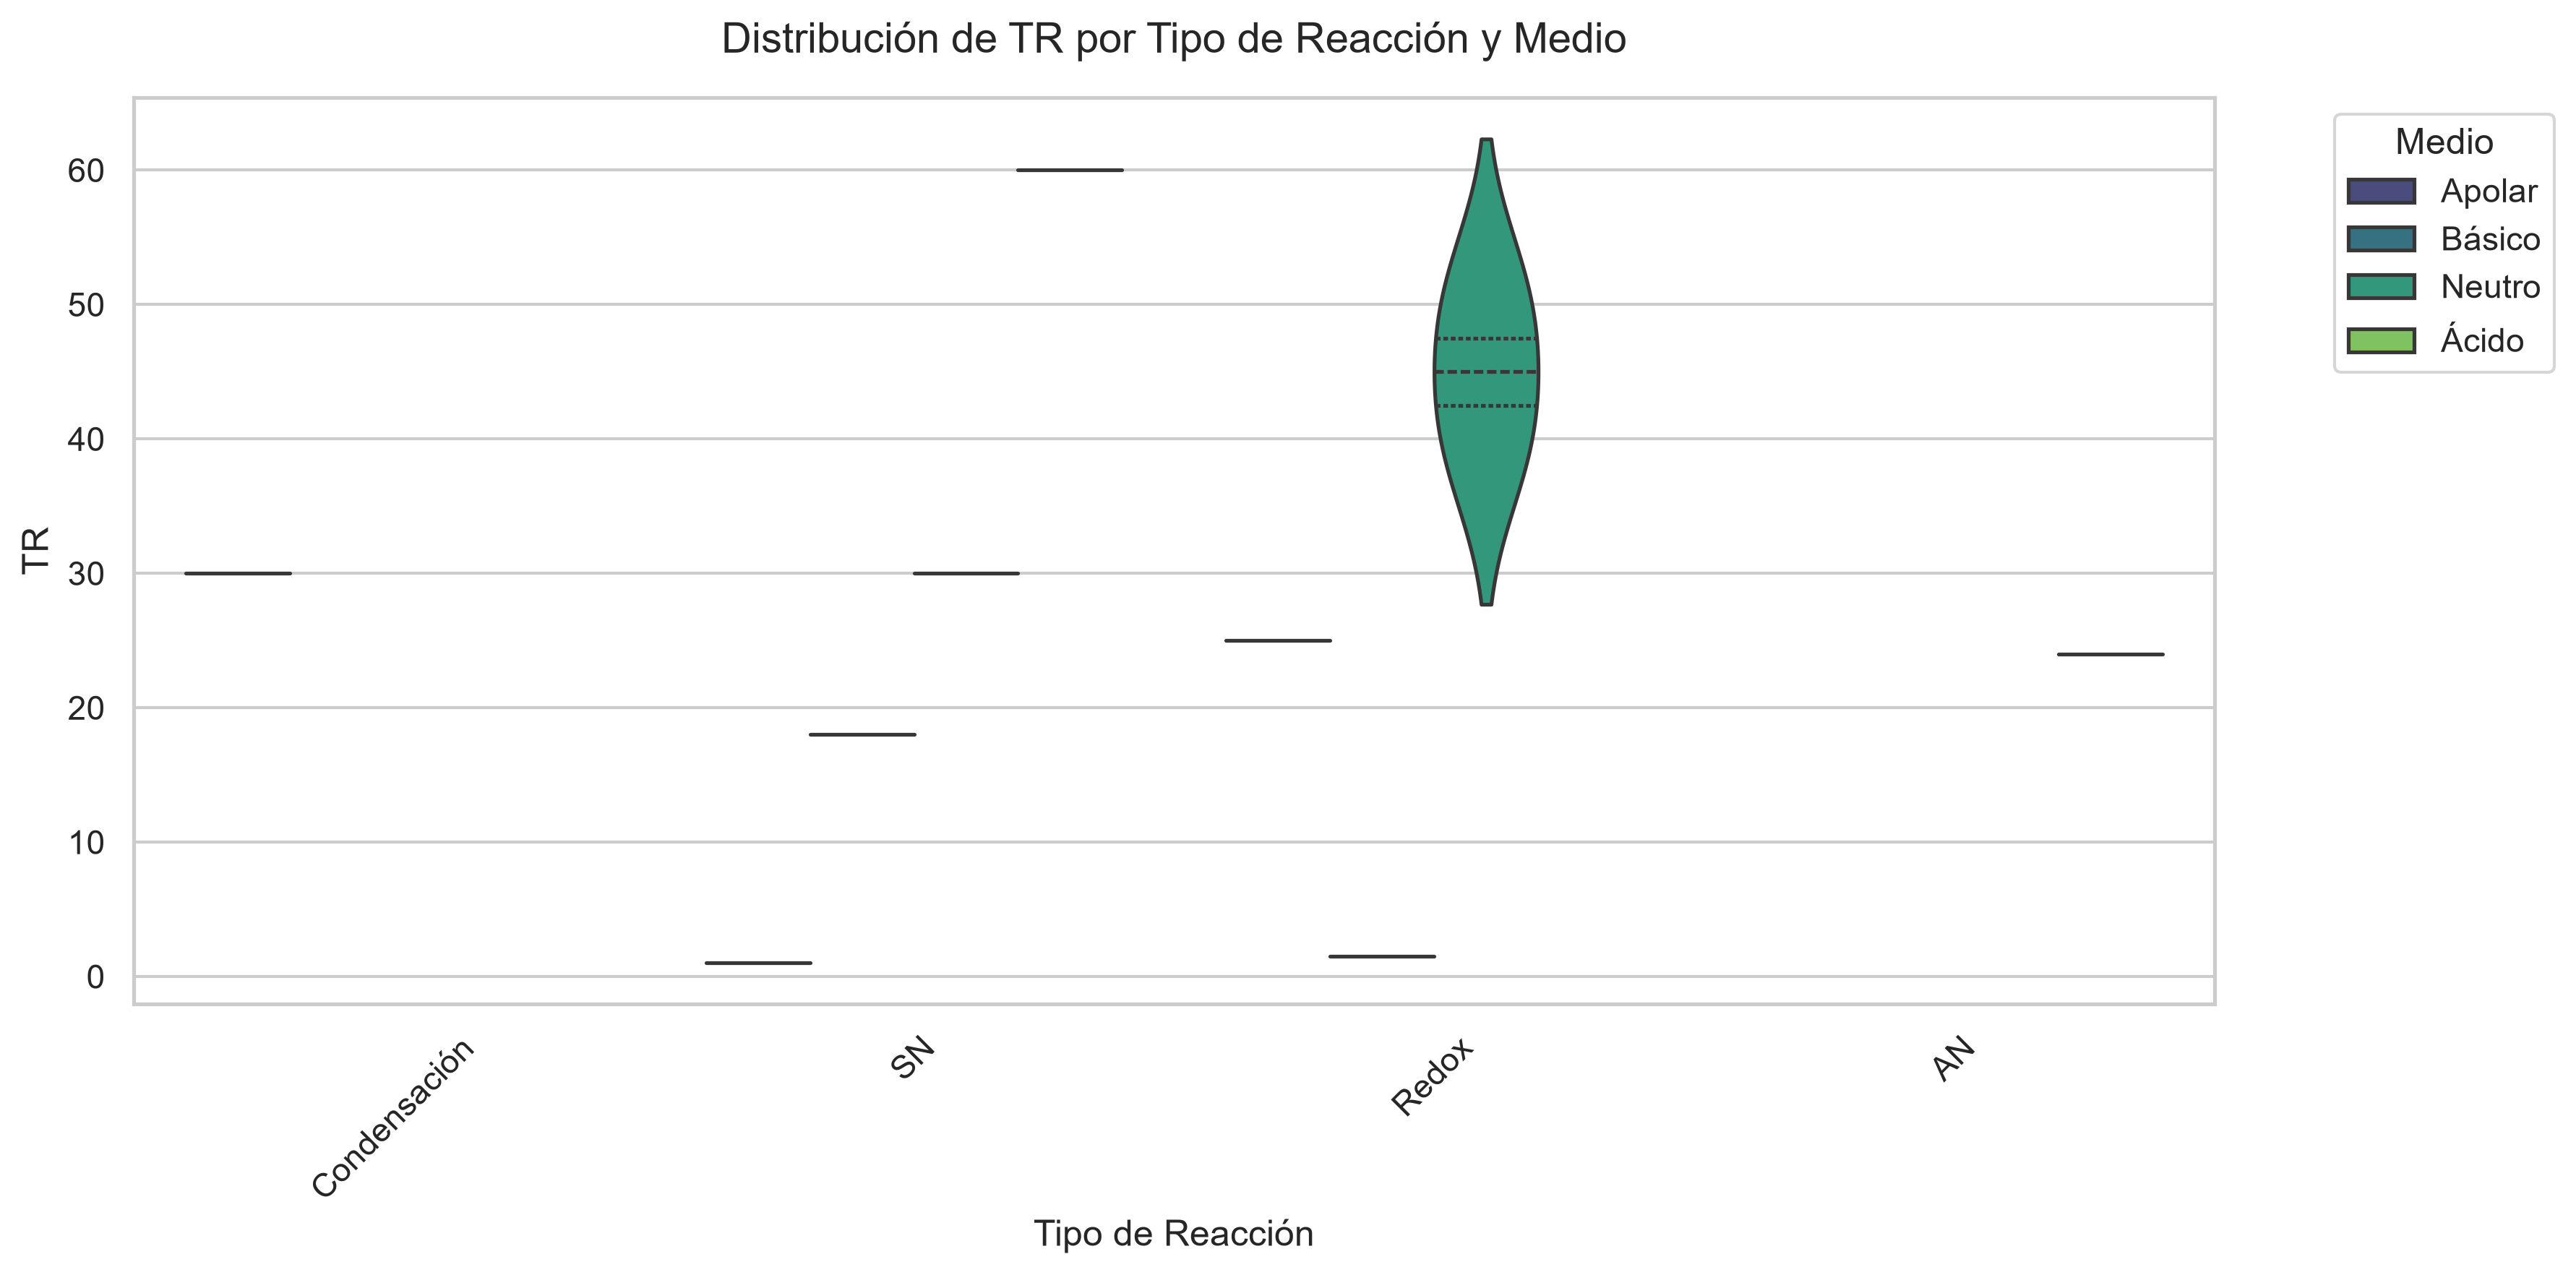
\includegraphics[width=\columnwidth]{07_violin_TR_tipo_medio.png}
	\caption{Distribución (violín) de TR por tipo de reacción y medio.}
	\label{fig:violin}
\end{figure}

\begin{figure}[htbp]
	\centering
	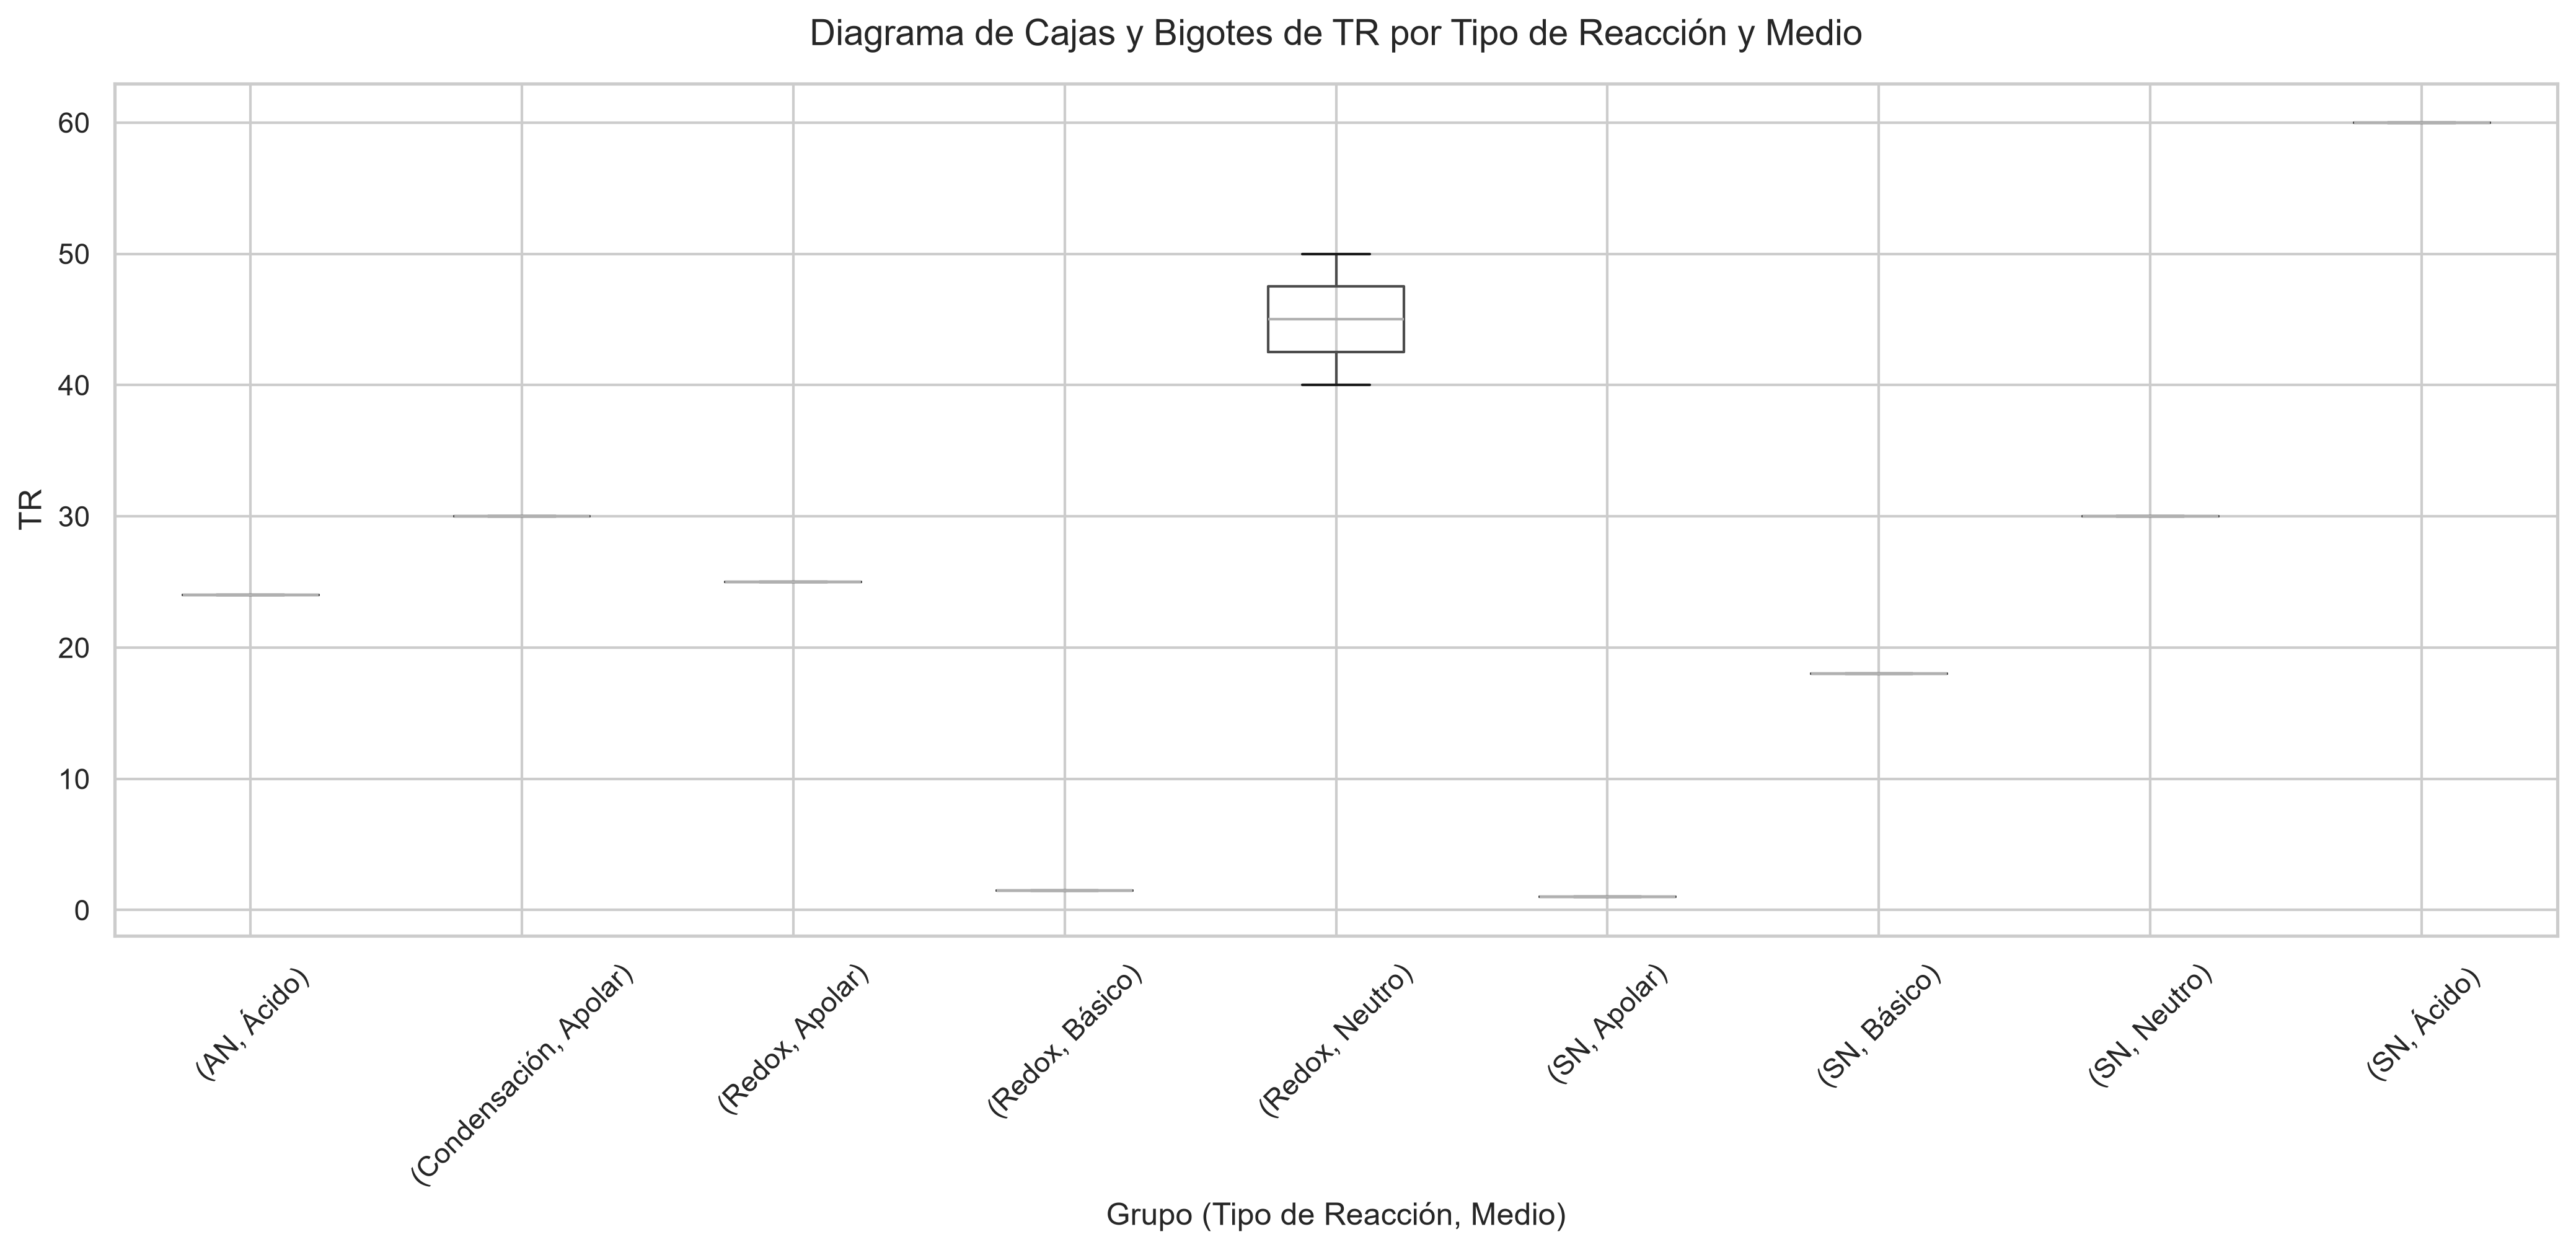
\includegraphics[width=\columnwidth]{08_boxplot_TR_tipo_medio.png}
	\caption{Diagrama de cajas y bigotes de TR por tipo de reacción y medio.}
	\label{fig:boxplot}
\end{figure}

\begin{figure}[htbp]
	\centering
	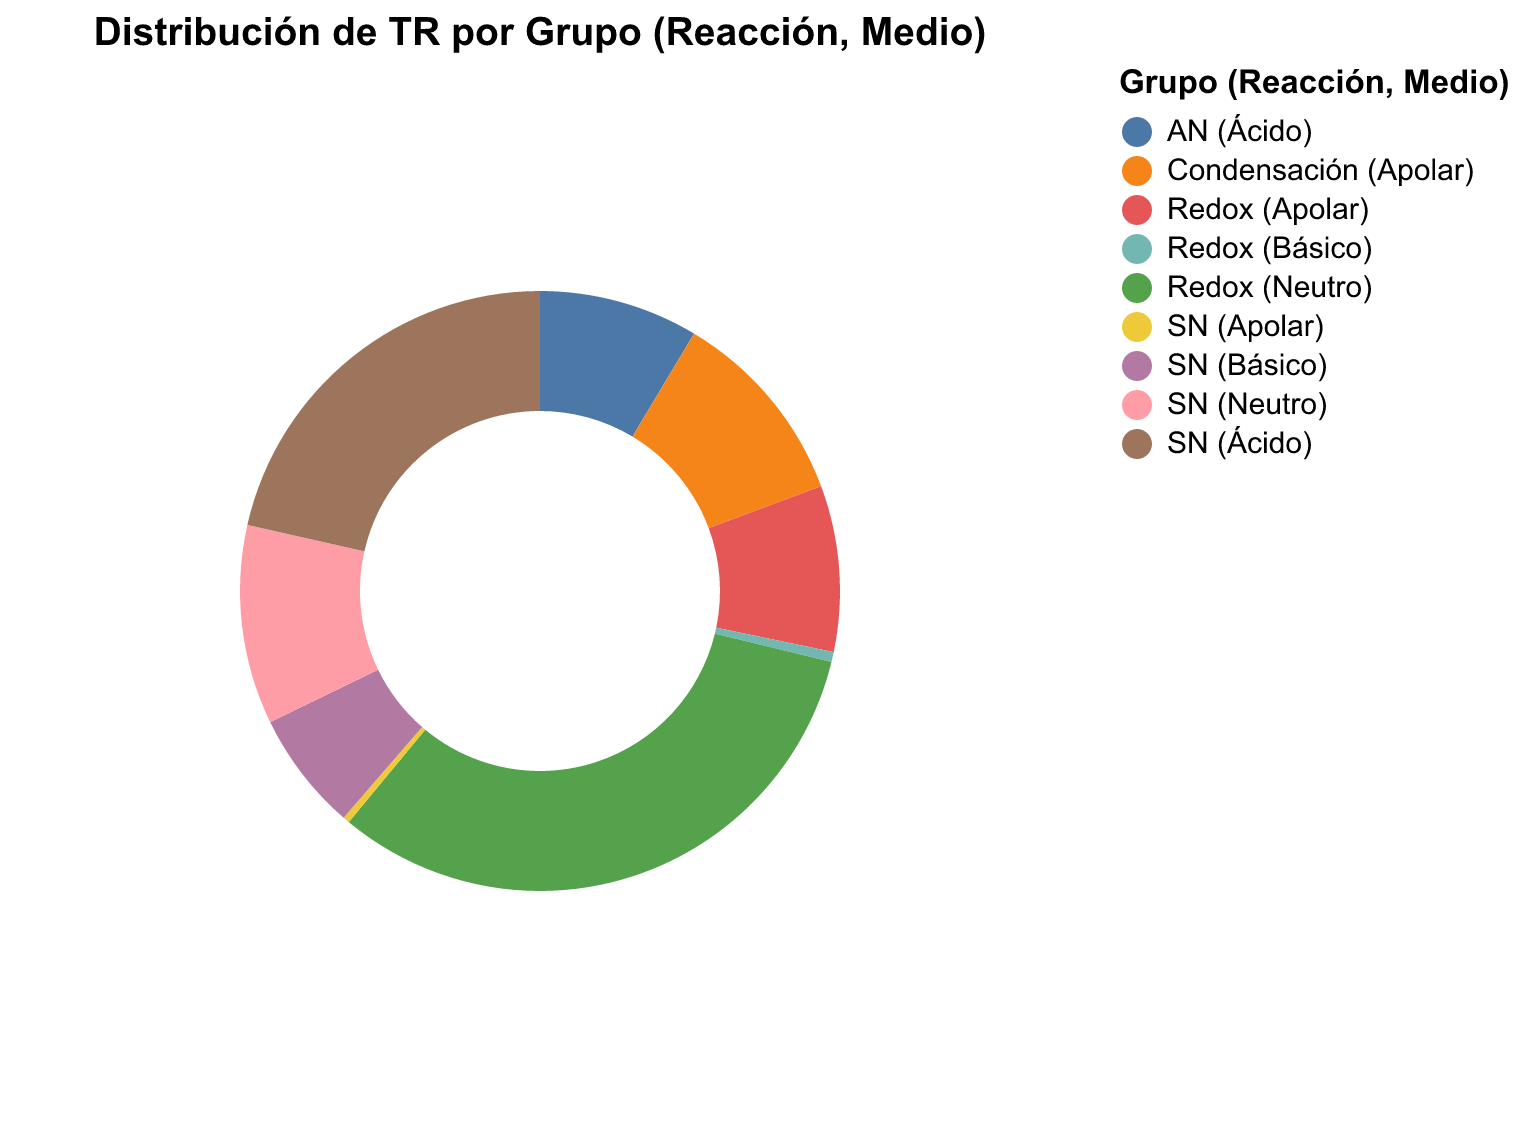
\includegraphics[width=0.9\columnwidth]{10_dona_TR_grupo.png}
	\caption{Participación de TR por grupo (tipo de reacción, medio).}
	\label{fig:dona}
\end{figure}

\section{Conclusiones y Perspectiva}
\fontsize{12}{14}\selectfont
% TODO (Valentina): 3--5 conclusiones que respondan al objetivo de la introducción,
% cada una sustentada en una figura o en la Tabla~\ref{tab:propiedades}.
\textit{[Redacción pendiente.]}

%  Contenido: Metodología, Análisis Gráfico (Colab/Conda) y Conclusiones
%
%  Reglas para editar sin romper la compilación:
%   * NO escribir \documentclass, \begin{document} ni \end{document} aquí.
%   * Las figuras están en ../imagenes/ y se llaman sólo por su nombre
%     (main.tex ya define \graphicspath{{imagenes/}}).
%   * Referenciar figuras con Figura~\ref{fig:...}, nunca "la figura de abajo".
% =====================================================================

\section{Metodología}
\fontsize{12}{14}\selectfont
% TODO (Valentina): pegar aquí la redacción de la metodología.

\subsection{Recolección de datos}
\textit{[Redacción pendiente: búsqueda en CAS-SciFinder, compuestos e indicadores asignados, consolidación en Excel con formato Tabla.]}

\subsection{Limpieza y procesamiento en Python}
\textit{[Redacción pendiente: Google Colab con Pandas, NumPy, Matplotlib, Seaborn y Plotly; filtrado de los compuestos de interés, conversión de comas decimales, tratamiento de valores nulos y atípicos.]}

\subsection{Análisis estadístico}
\textit{[Redacción pendiente: correlación de Spearman (no paramétrica, robusta a valores atípicos y relaciones monótonas no lineales), regresiones lineales con intervalo de confianza del 95\,\% y distribuciones por tipo de reacción y medio.]}

\section{Resultados y Discusión}
\fontsize{12}{14}\selectfont

\subsection{Correlación entre propiedades}
% TODO (Valentina): interpretar los coeficientes más fuertes (positivos y negativos).
La Figura~\ref{fig:heatmap} presenta la matriz de correlación de Spearman entre
las propiedades fisicoquímicas, y la Figura~\ref{fig:clustermap} agrupa
jerárquicamente las variables con comportamiento similar.
\textit{[Interpretación pendiente.]}

\begin{figure}[htbp]
	\centering
	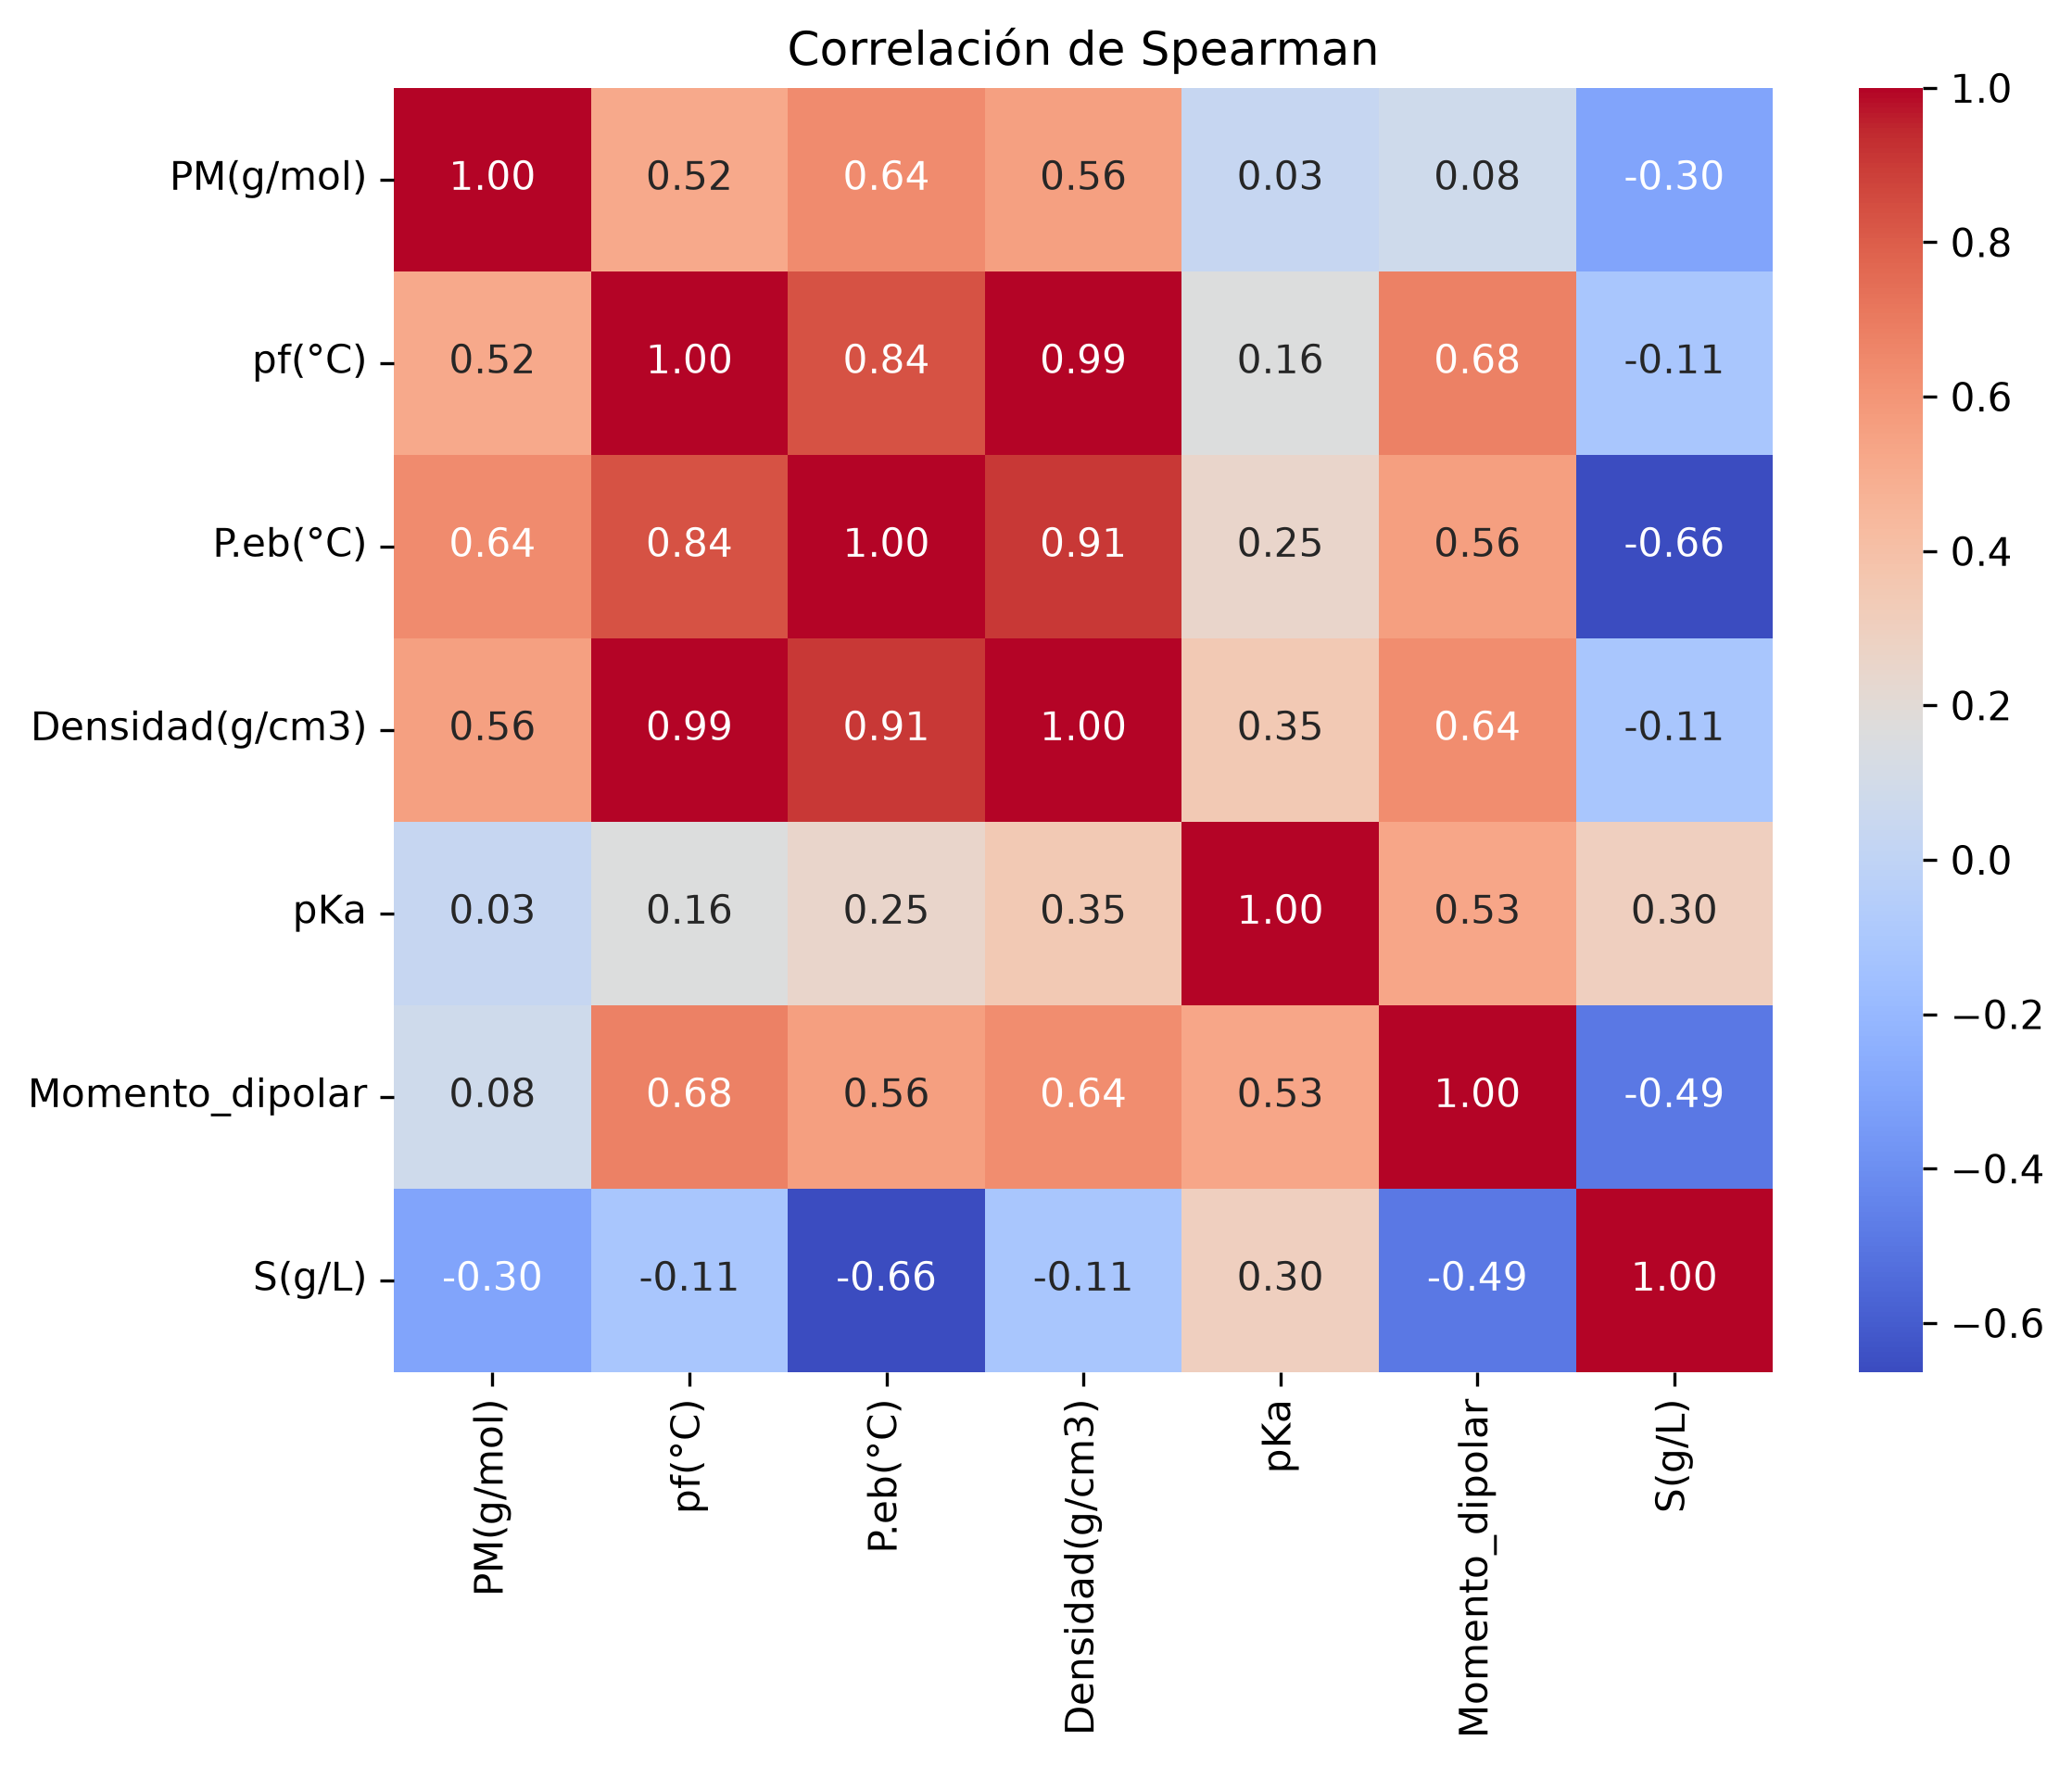
\includegraphics[width=\columnwidth]{01_heatmap_spearman.png}
	\caption{Matriz de correlación de Spearman entre las propiedades fisicoquímicas.}
	\label{fig:heatmap}
\end{figure}

\begin{figure}[htbp]
	\centering
	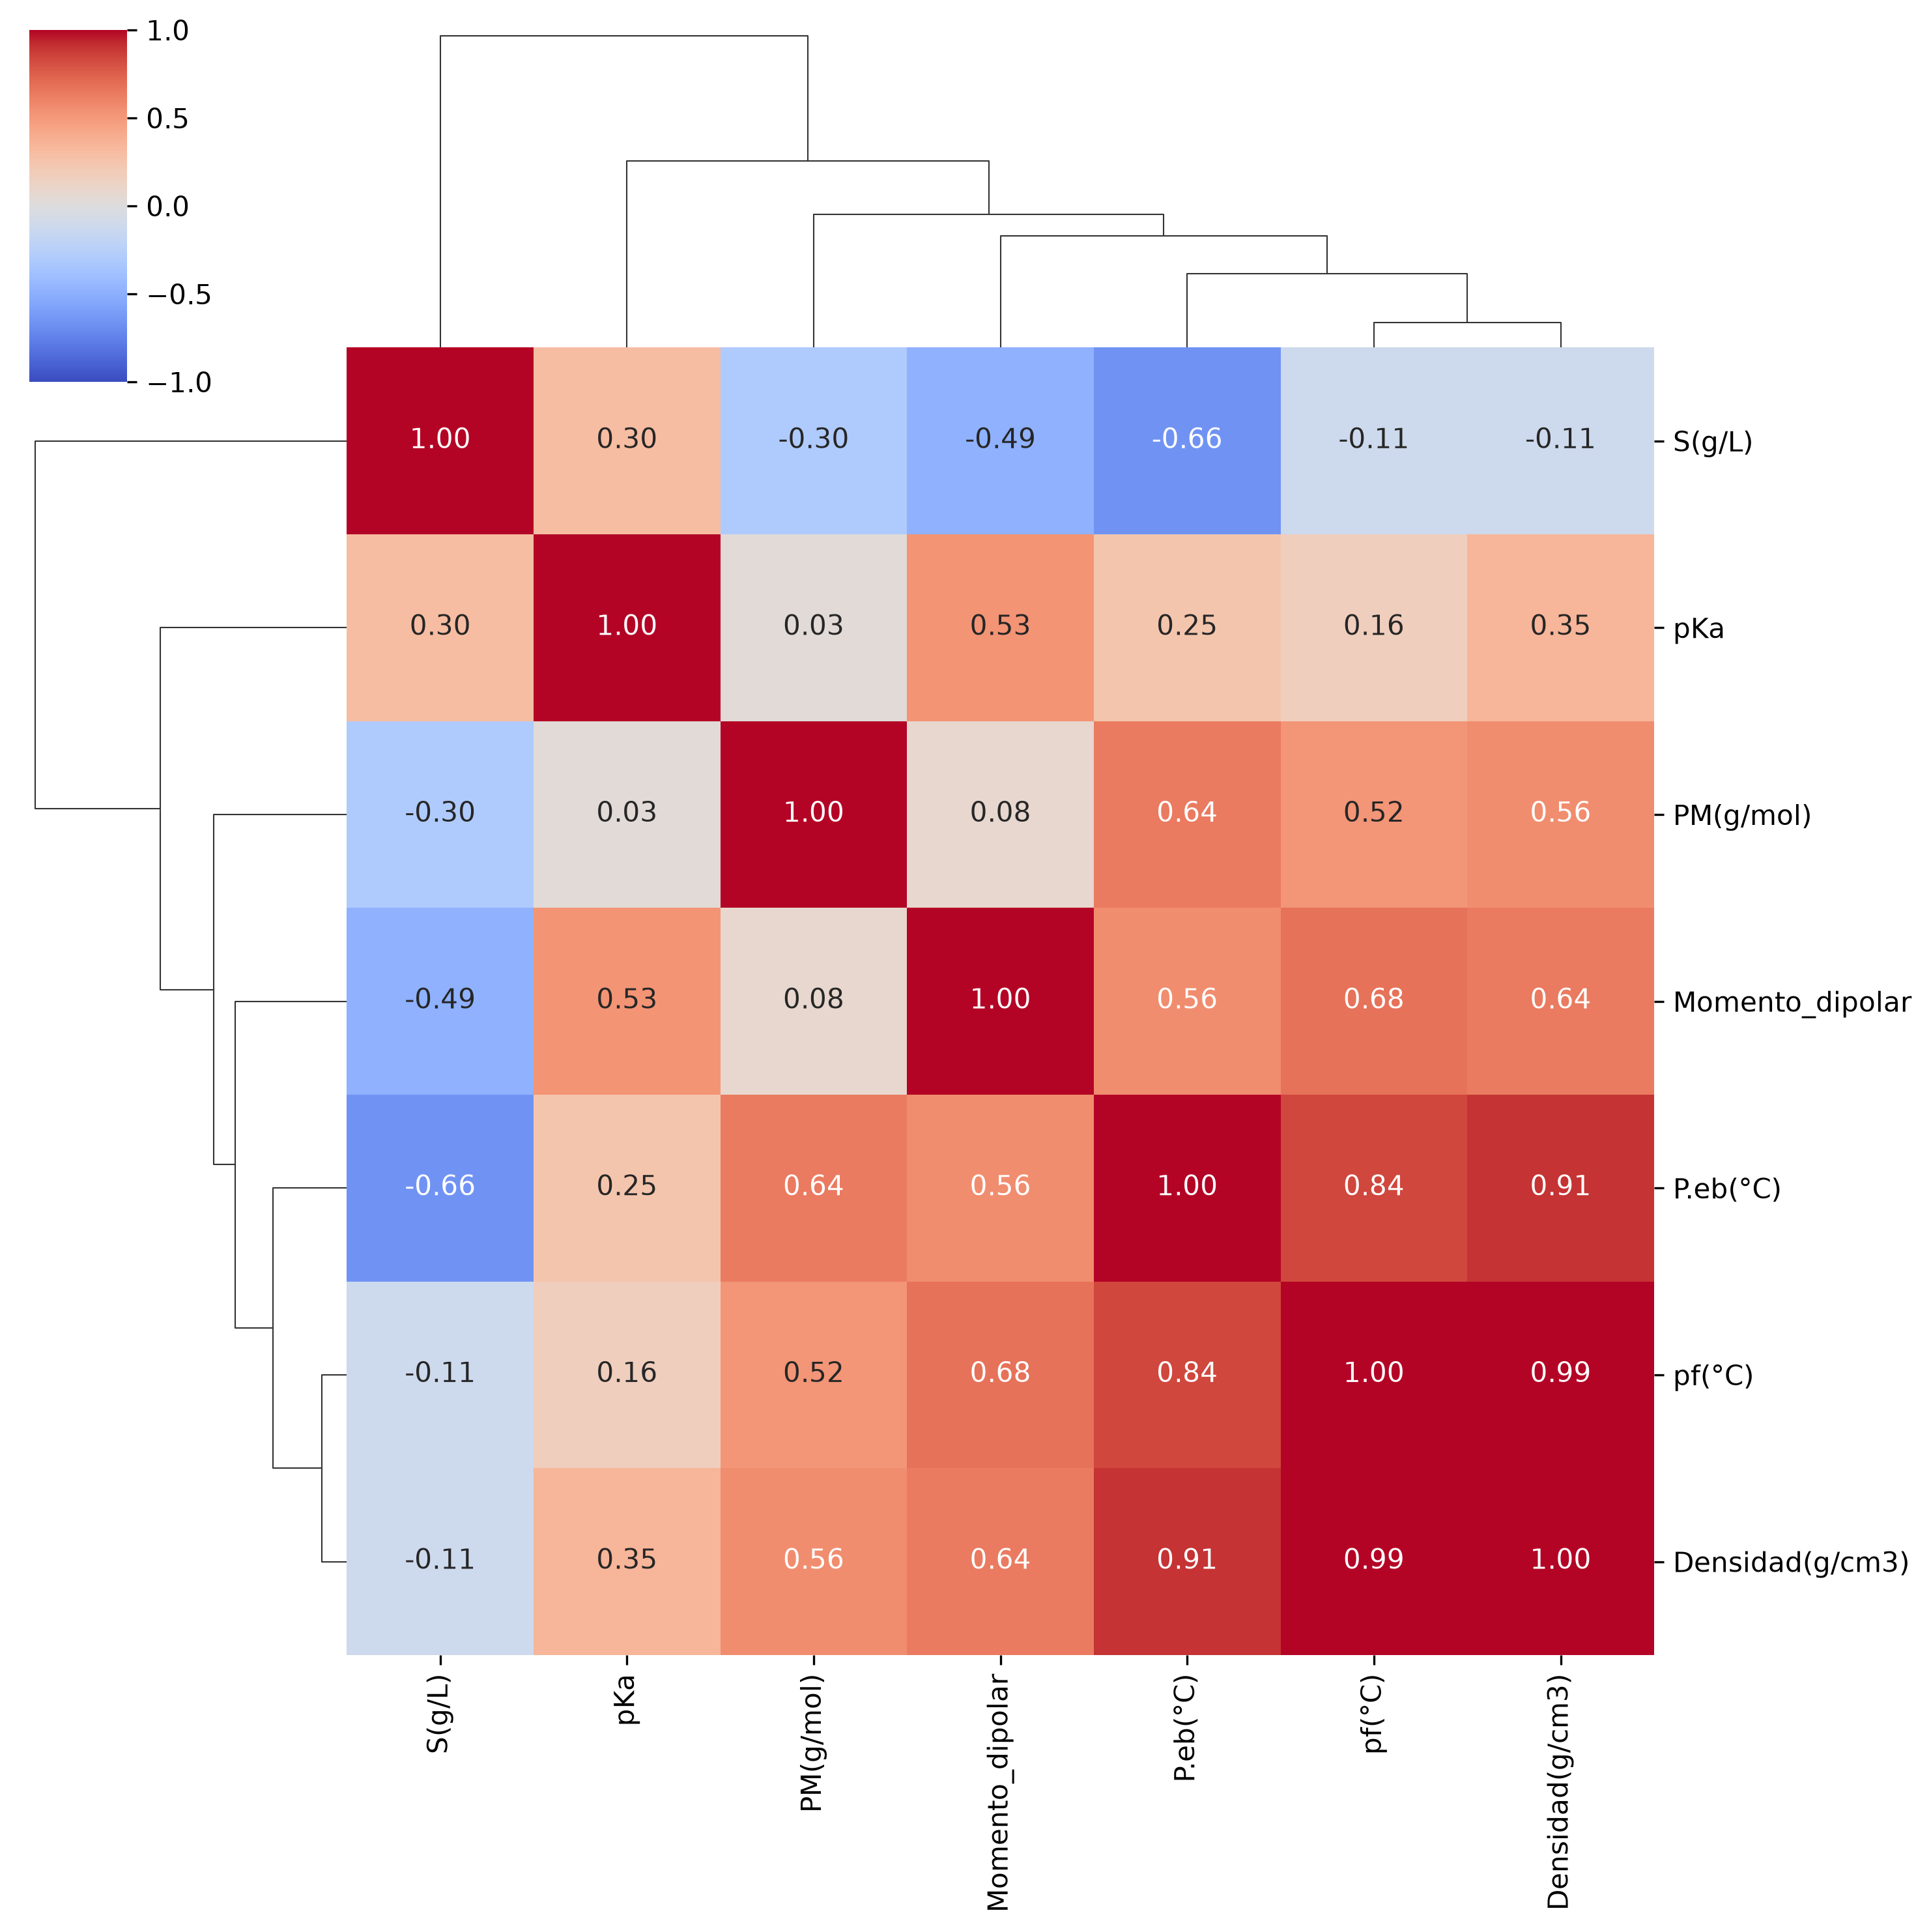
\includegraphics[width=\columnwidth]{02_clustermap_spearman.png}
	\caption{Mapa de agrupamiento jerárquico de la correlación de Spearman.}
	\label{fig:clustermap}
\end{figure}

\subsection{Tendencias entre propiedades}
% TODO (Valentina): discutir cada regresión en términos de fuerzas intermoleculares.
Las Figuras~\ref{fig:pf-dens}--\ref{fig:dip-peb} muestran las regresiones
lineales entre pares de propiedades, con su intervalo de confianza.
\textit{[Interpretación pendiente.]}

\begin{figure}[htbp]
	\centering
	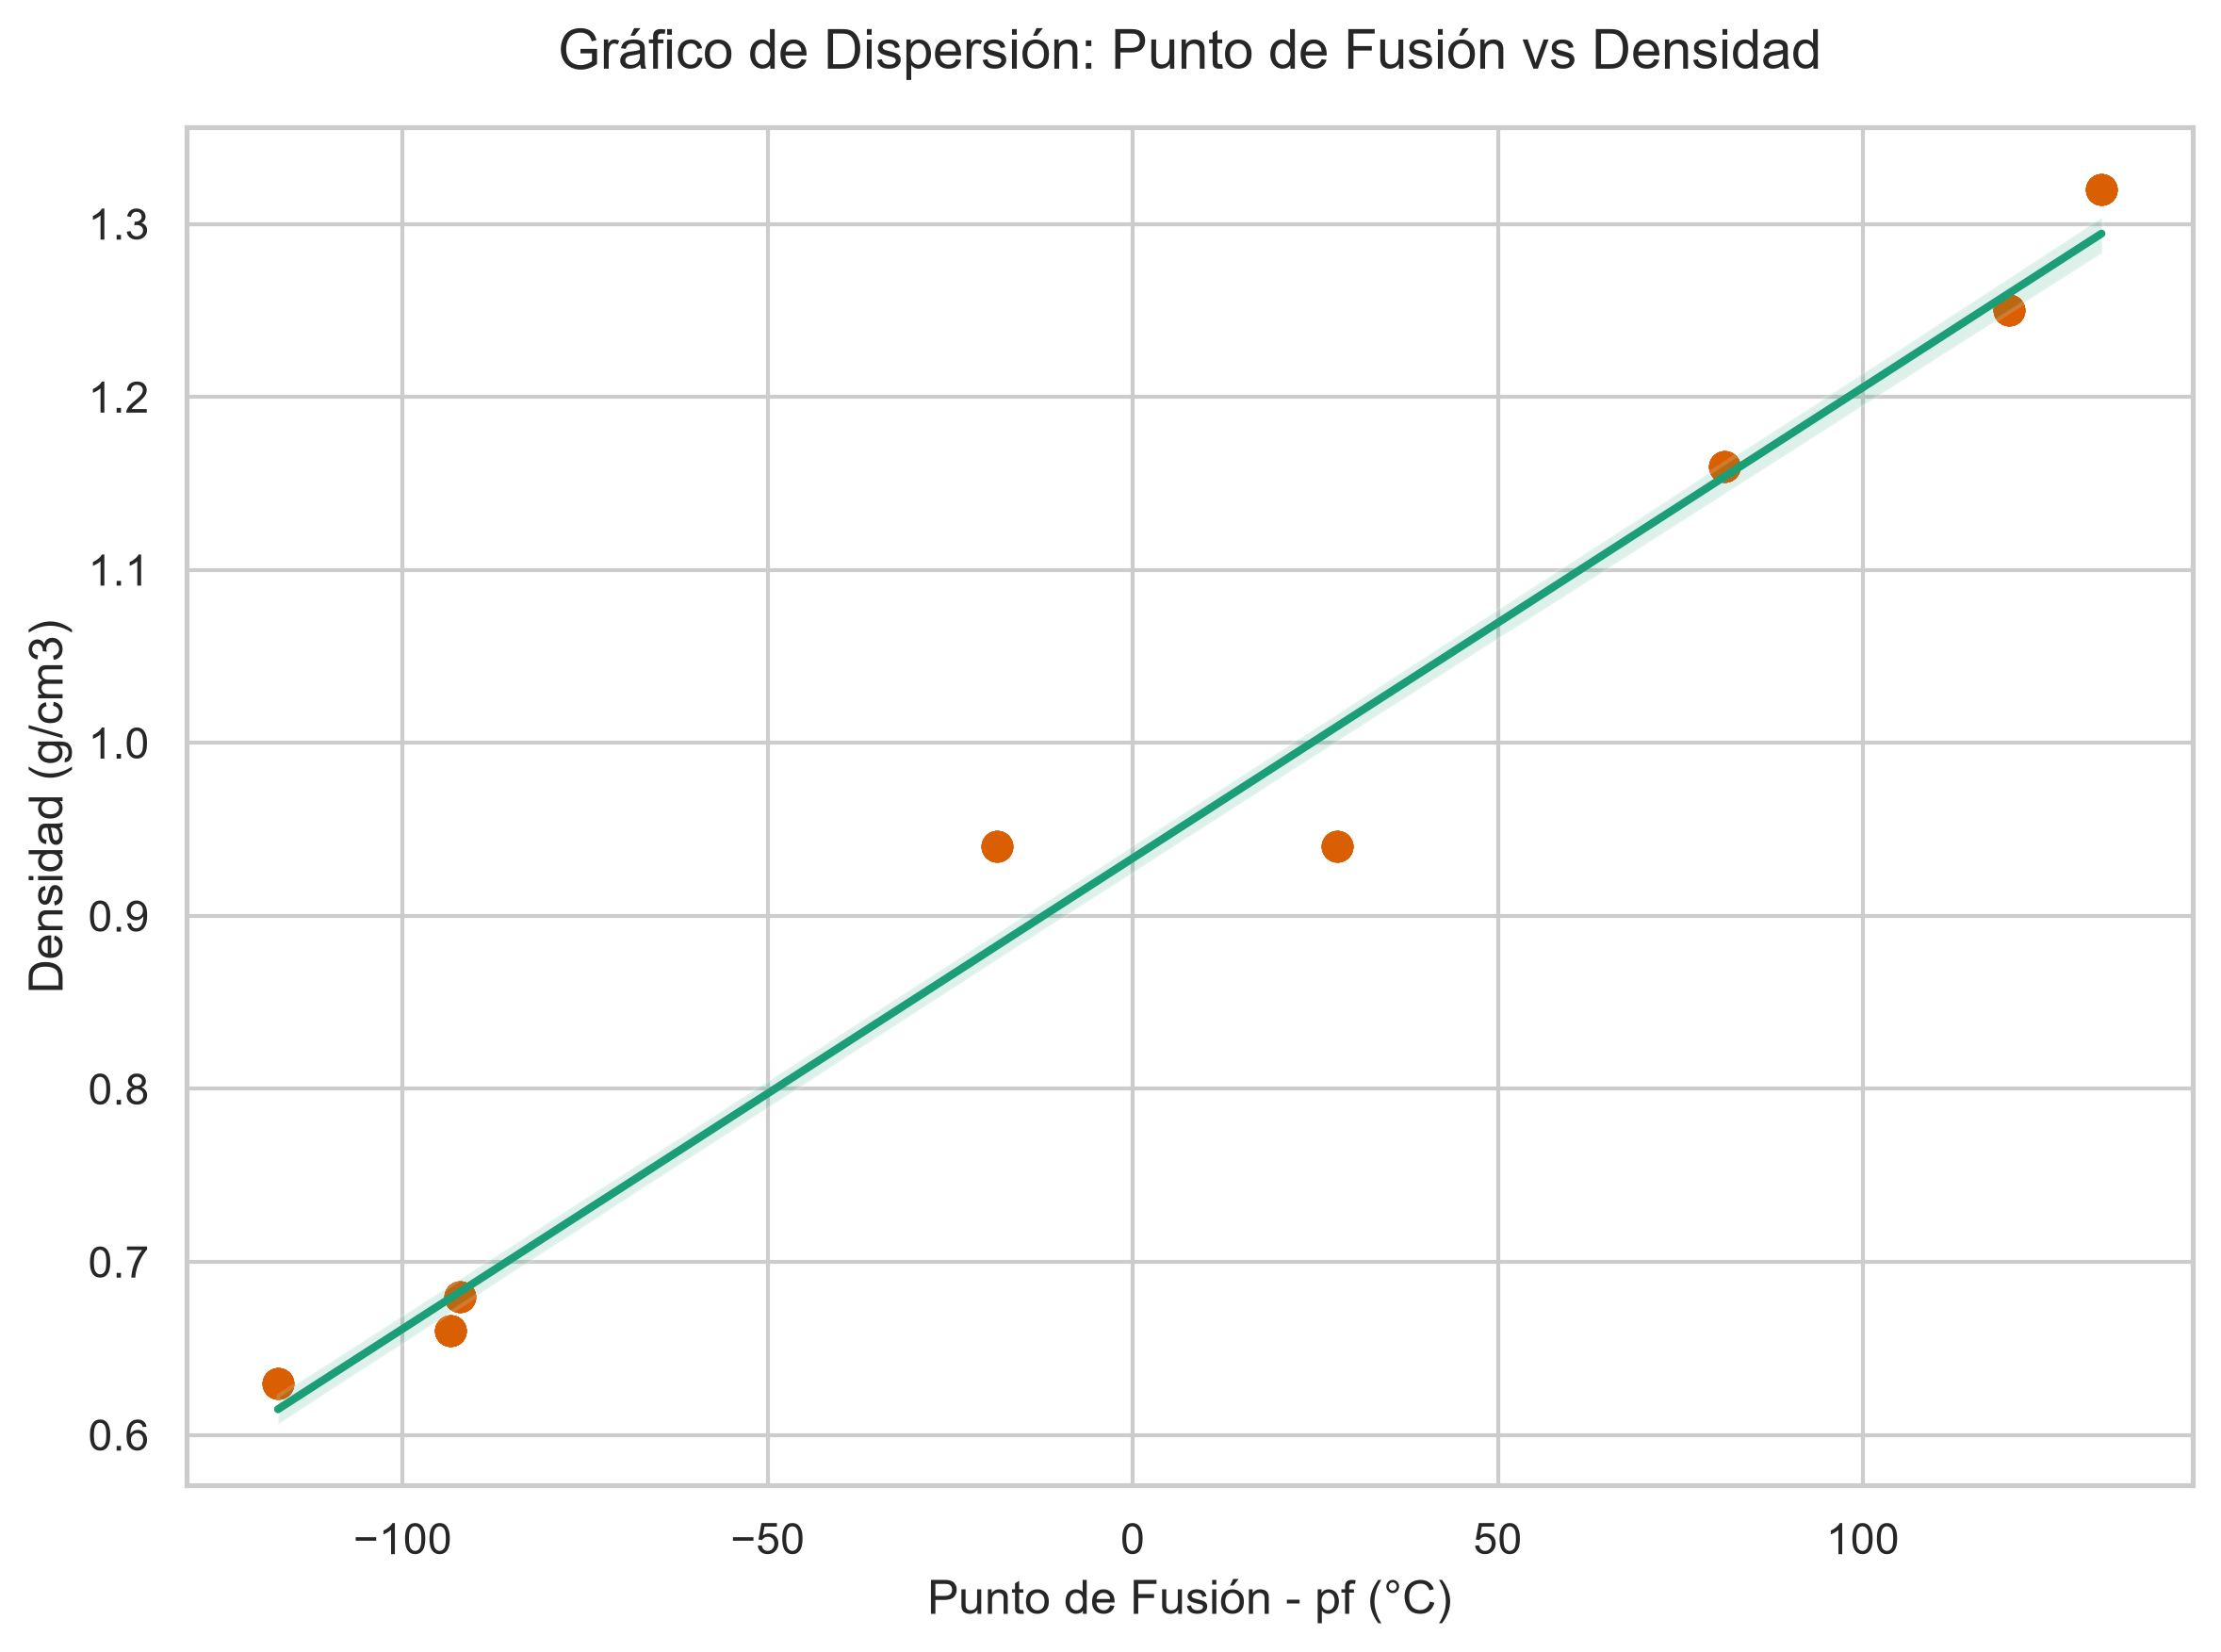
\includegraphics[width=\columnwidth]{03_reg_pf_vs_densidad.png}
	\caption{Punto de fusión frente a densidad.}
	\label{fig:pf-dens}
\end{figure}

\begin{figure}[htbp]
	\centering
	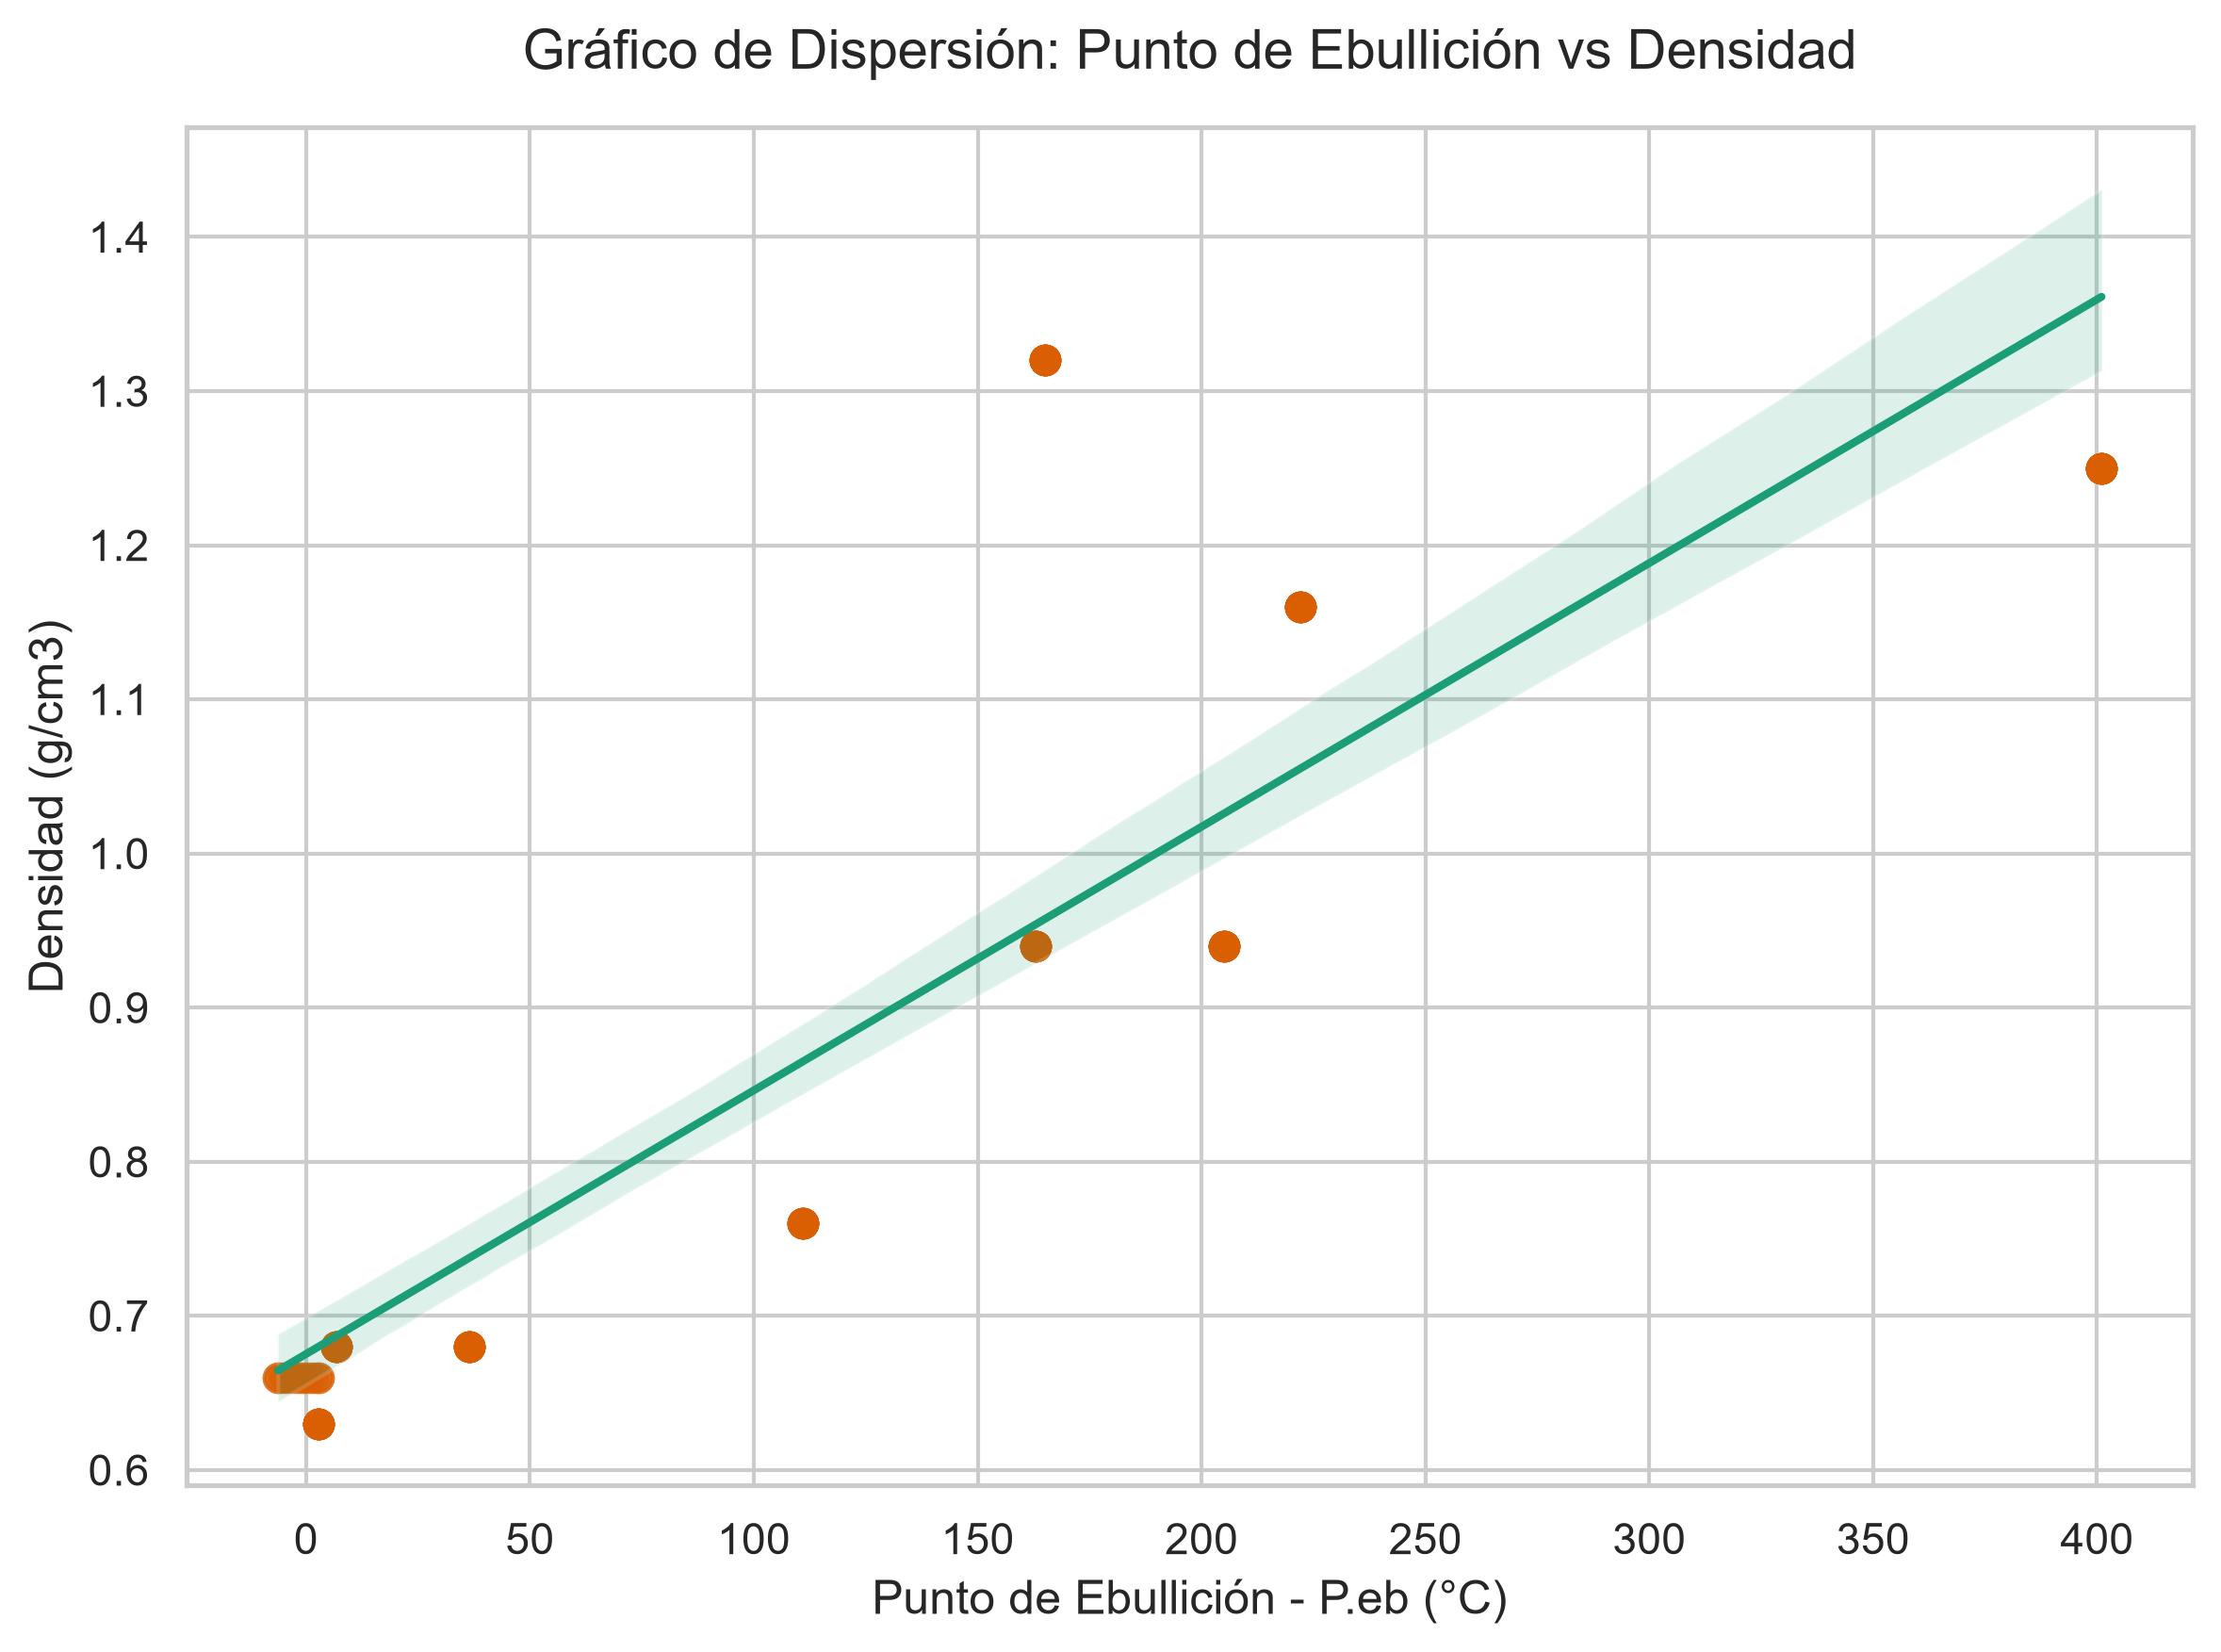
\includegraphics[width=\columnwidth]{04_reg_peb_vs_densidad.png}
	\caption{Punto de ebullición frente a densidad.}
	\label{fig:peb-dens}
\end{figure}

\begin{figure}[htbp]
	\centering
	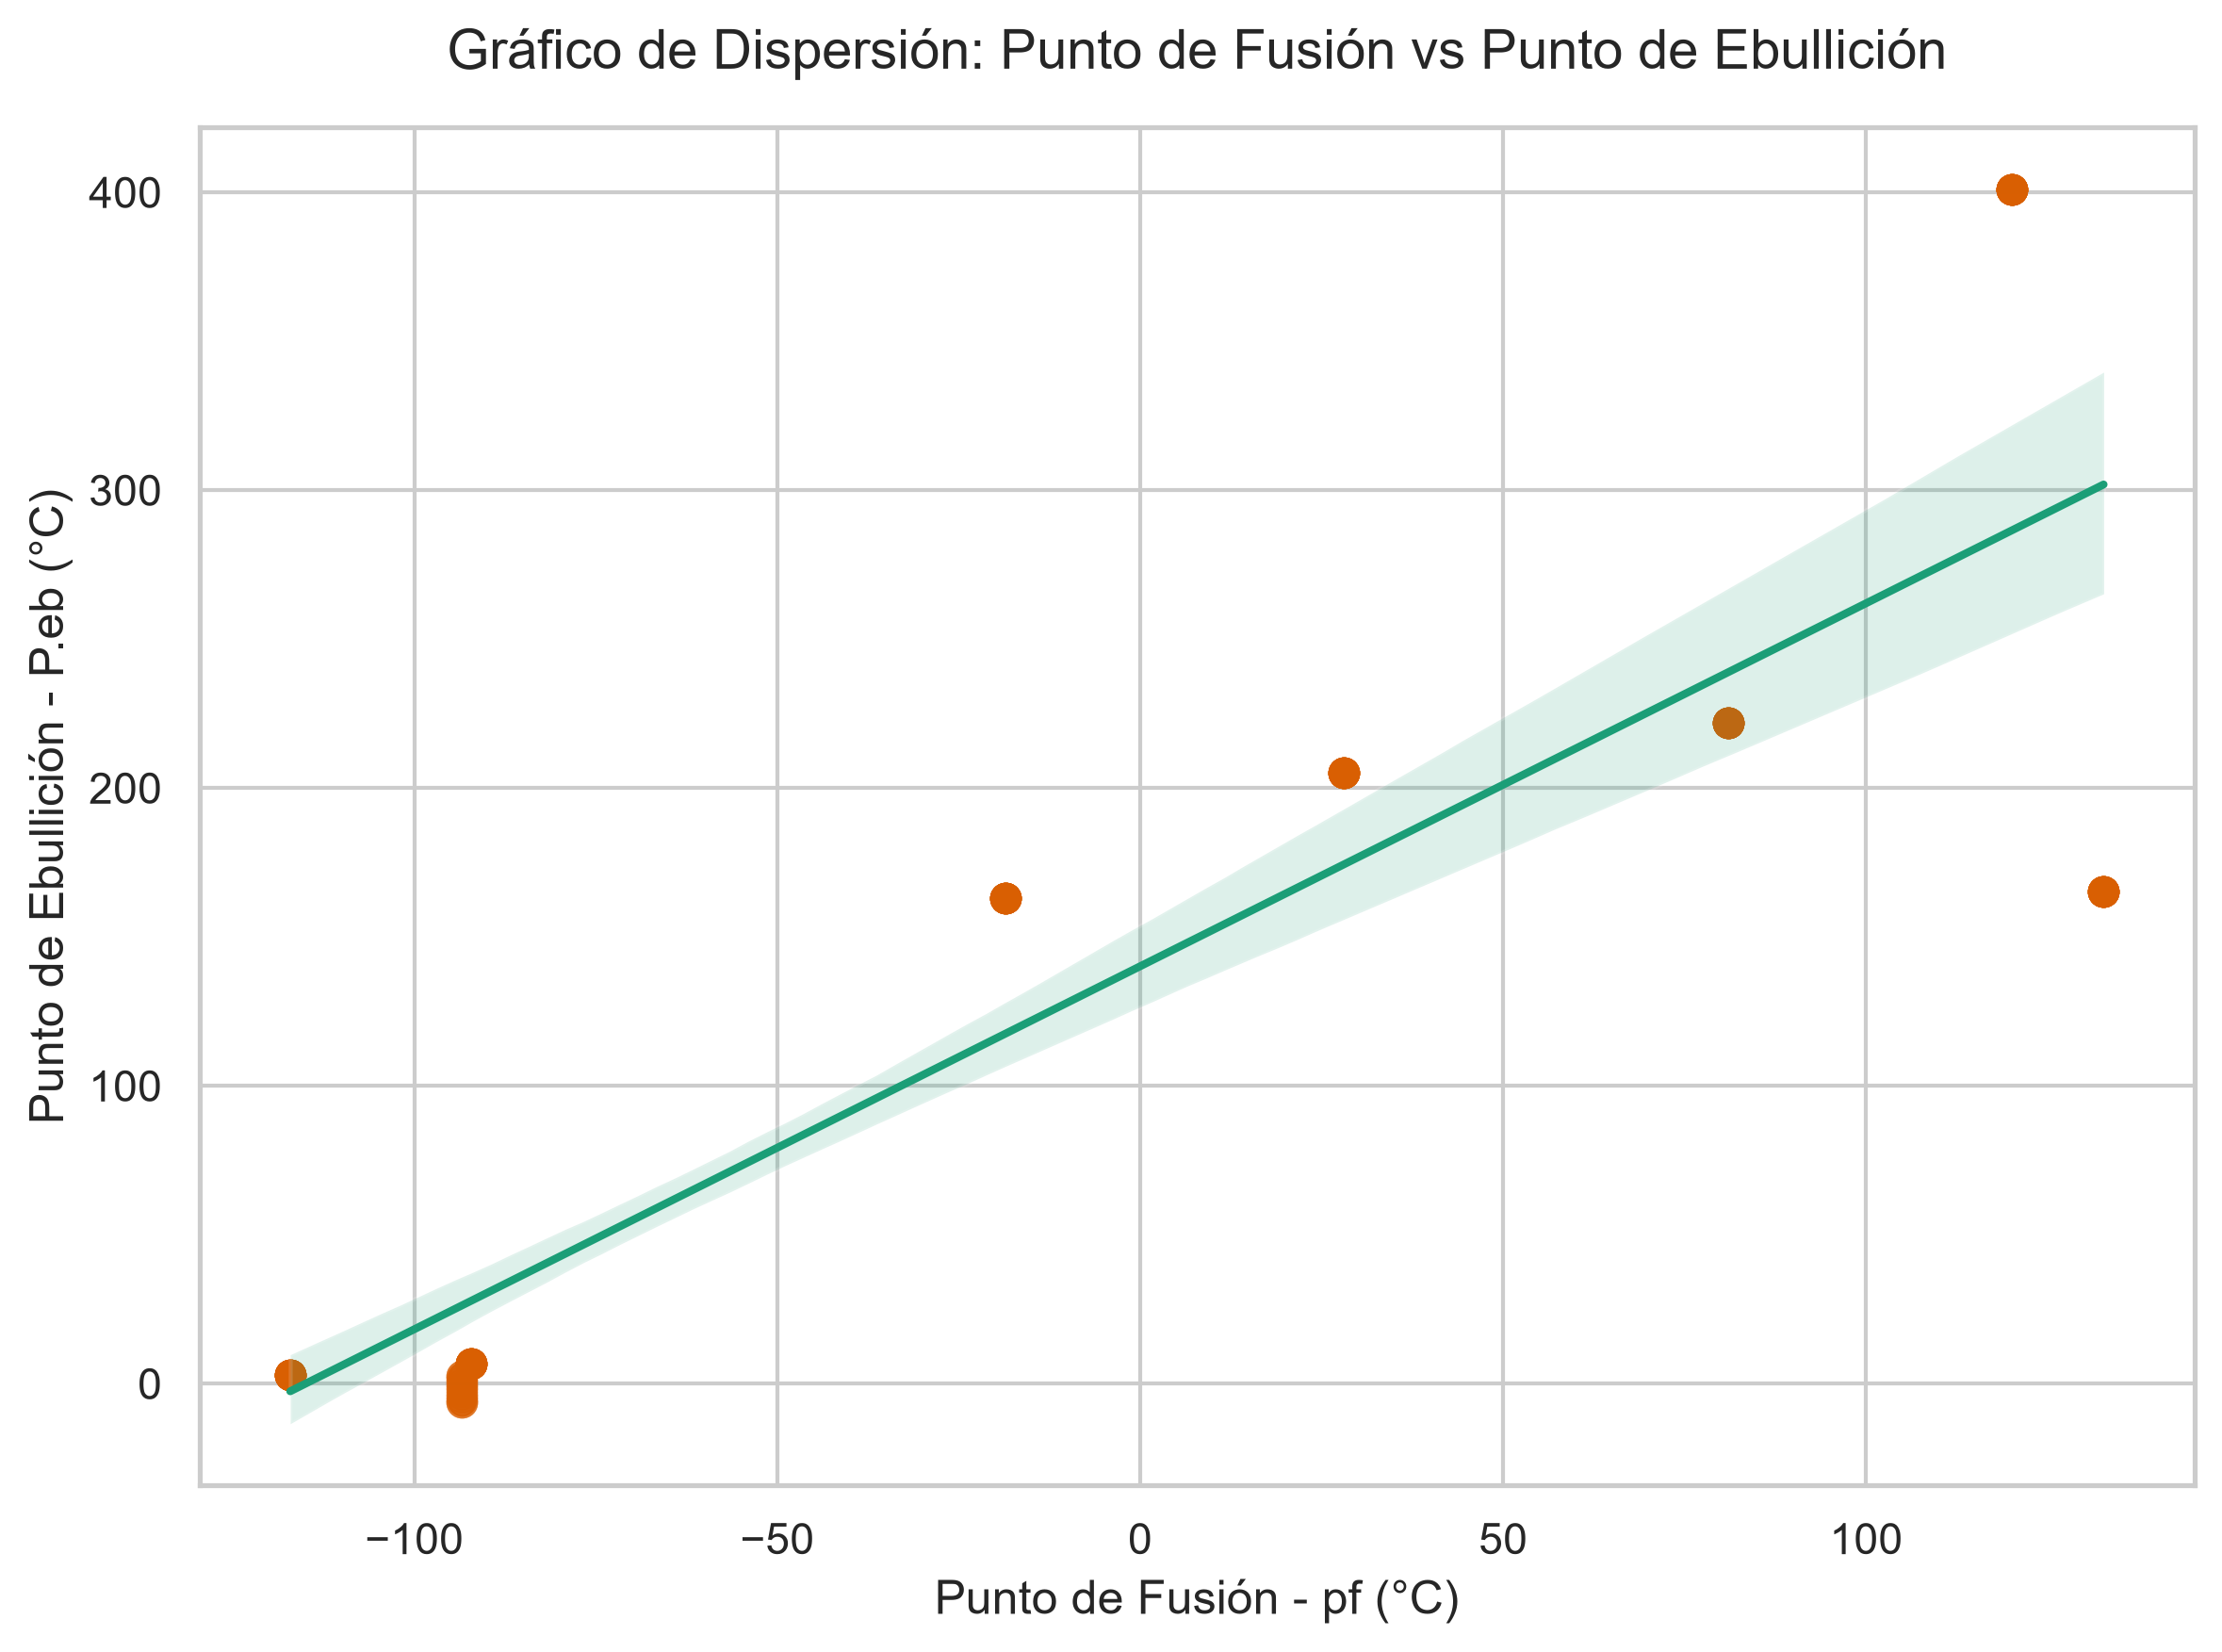
\includegraphics[width=\columnwidth]{05_reg_pf_vs_peb.png}
	\caption{Punto de fusión frente a punto de ebullición.}
	\label{fig:pf-peb}
\end{figure}

\begin{figure}[htbp]
	\centering
	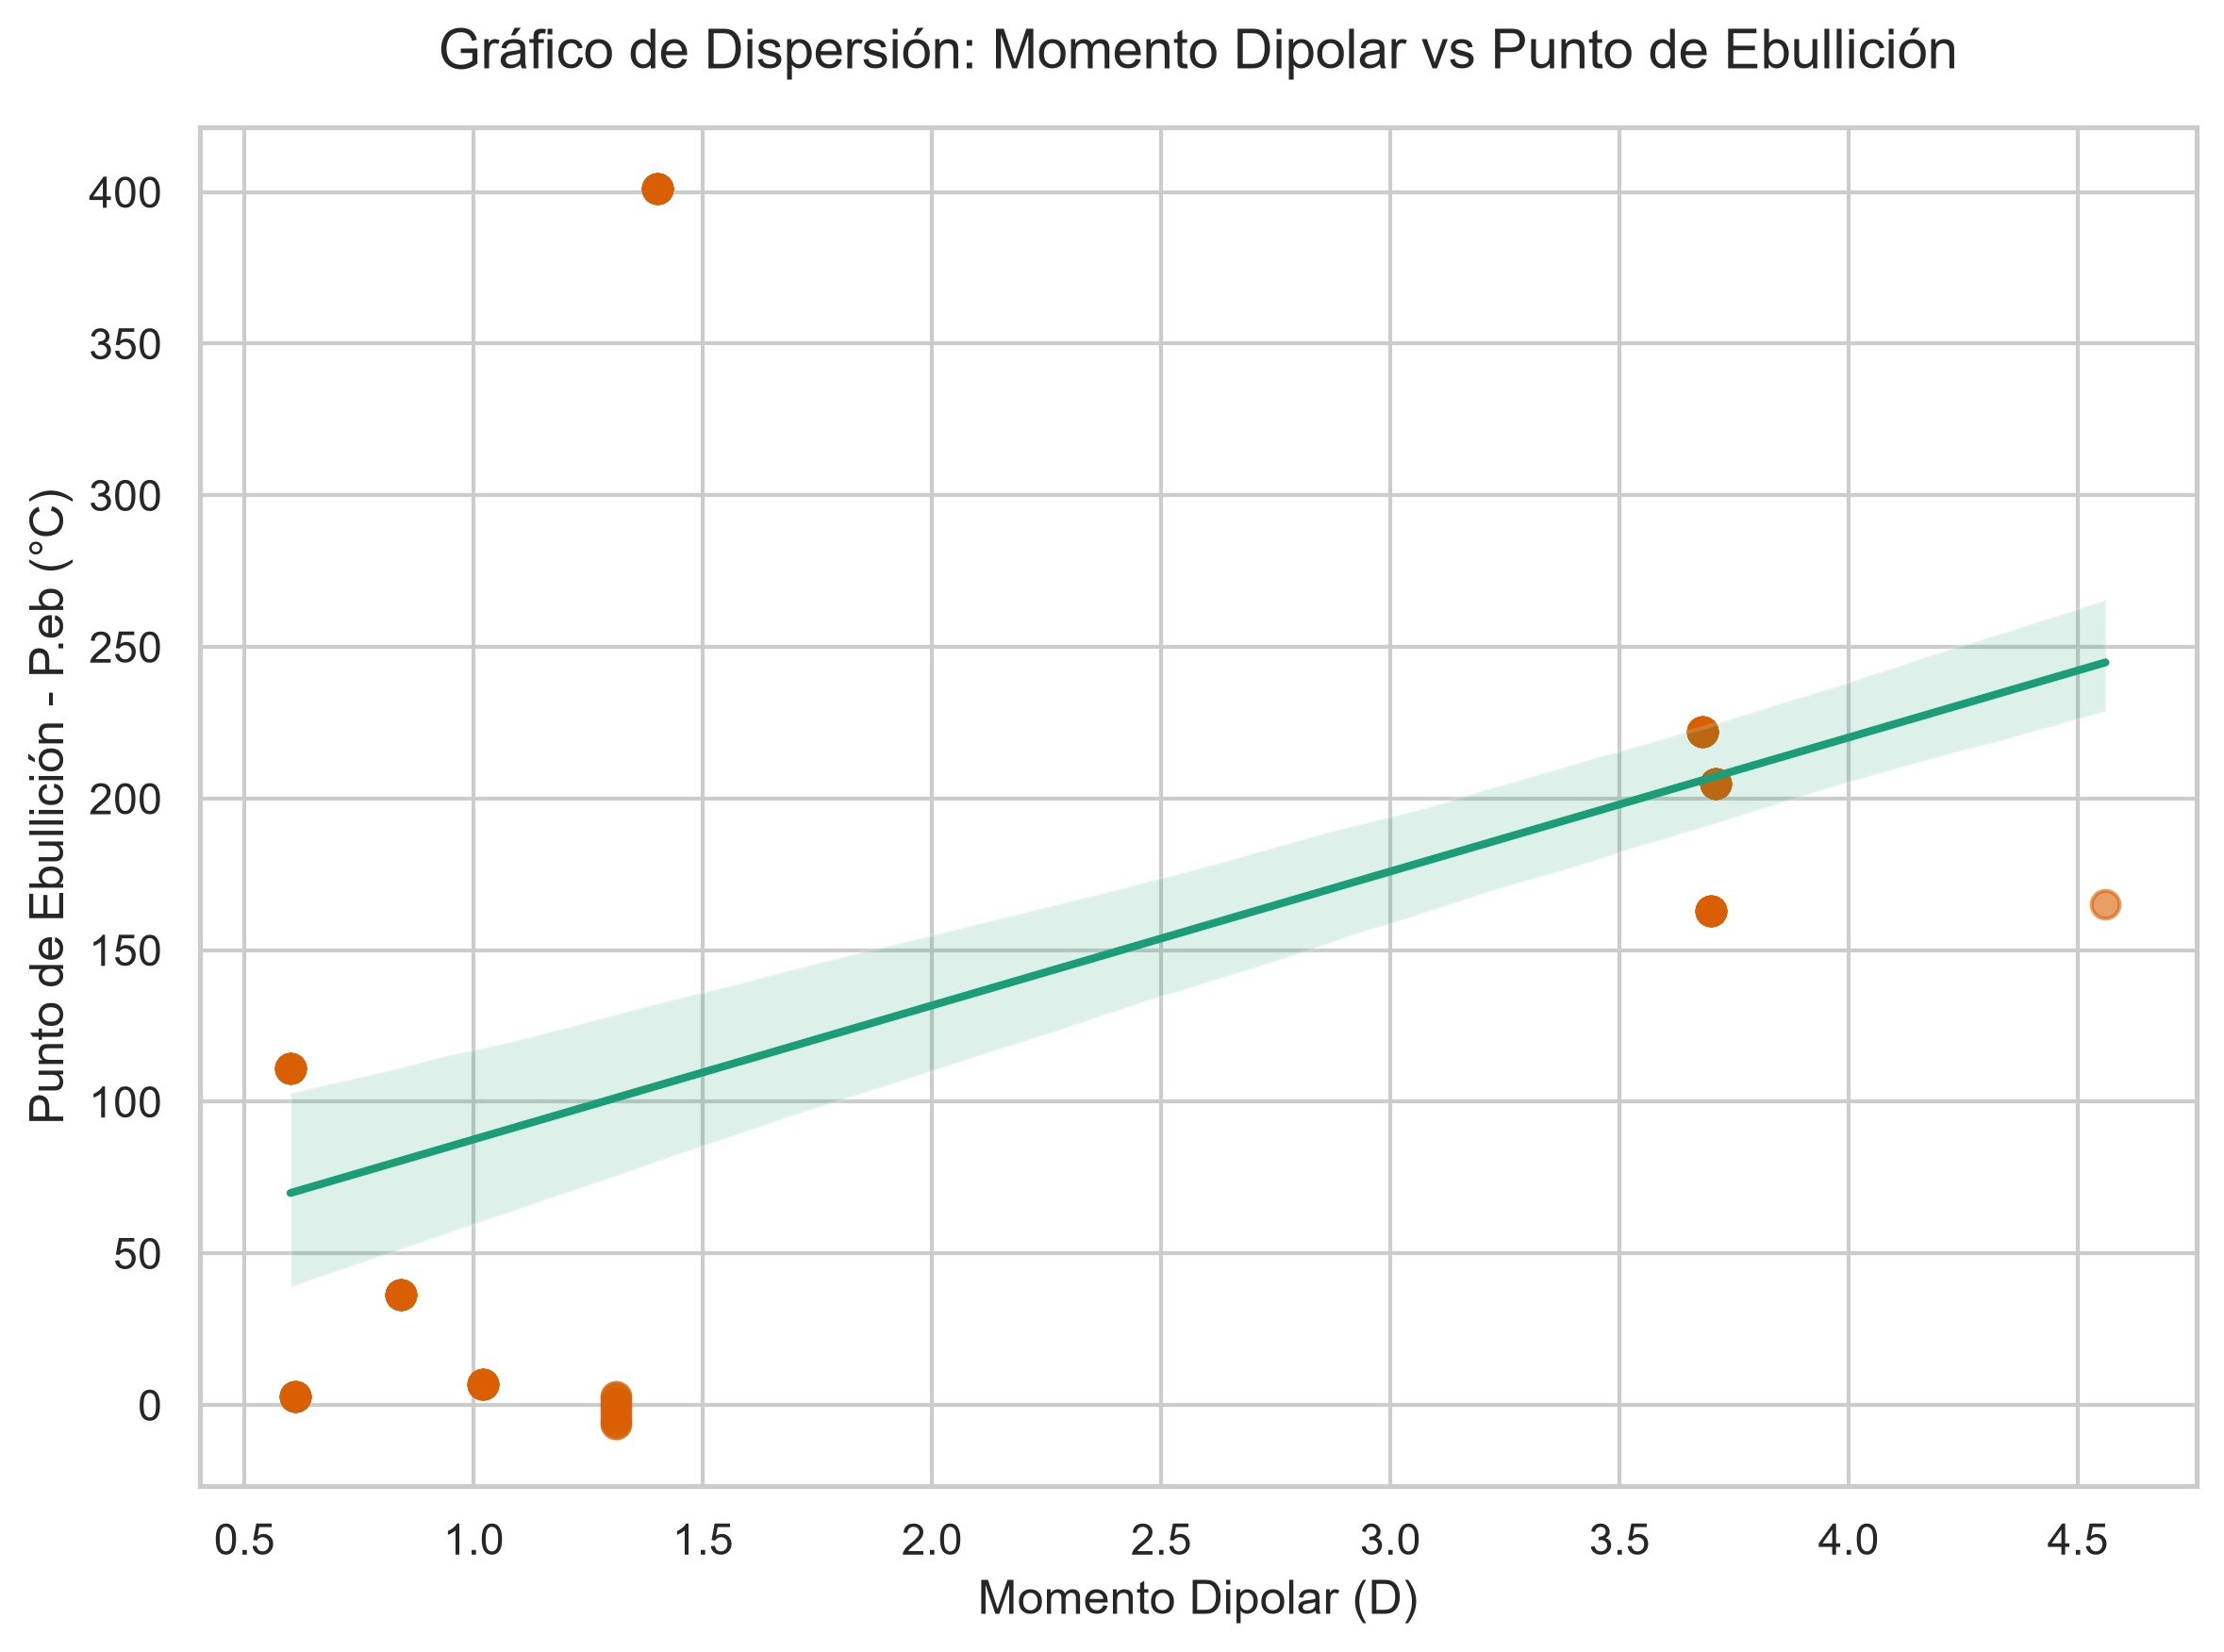
\includegraphics[width=\columnwidth]{06_reg_dipolo_vs_peb.png}
	\caption{Momento dipolar frente a punto de ebullición.}
	\label{fig:dip-peb}
\end{figure}

\subsection{Exploración interactiva con Plotly}
% TODO (Valentina): interpretar; idea central: a igual PM, los compuestos con
% enlace N--H (donadores de puente de H) hierven mucho más alto.
Las Figuras~\ref{fig:burbujas}--\ref{fig:dens-sol} se generaron con Plotly,
una fila por compuesto; sus versiones HTML permiten inspeccionar cada molécula
con el cursor. En la Figura~\ref{fig:burbujas}, trimetilamina
(\SI{2.8}{\degreeCelsius}) y N-metiletanamina (\SI{36.5}{\degreeCelsius}) tienen
el mismo peso molecular (\SI{59.11}{\gram\per\mole}): la diferencia se debe a que
sólo la segunda posee enlace N--H y forma puentes de hidrógeno.
\textit{[Interpretación pendiente.]}

\begin{figure}[htbp]
	\centering
	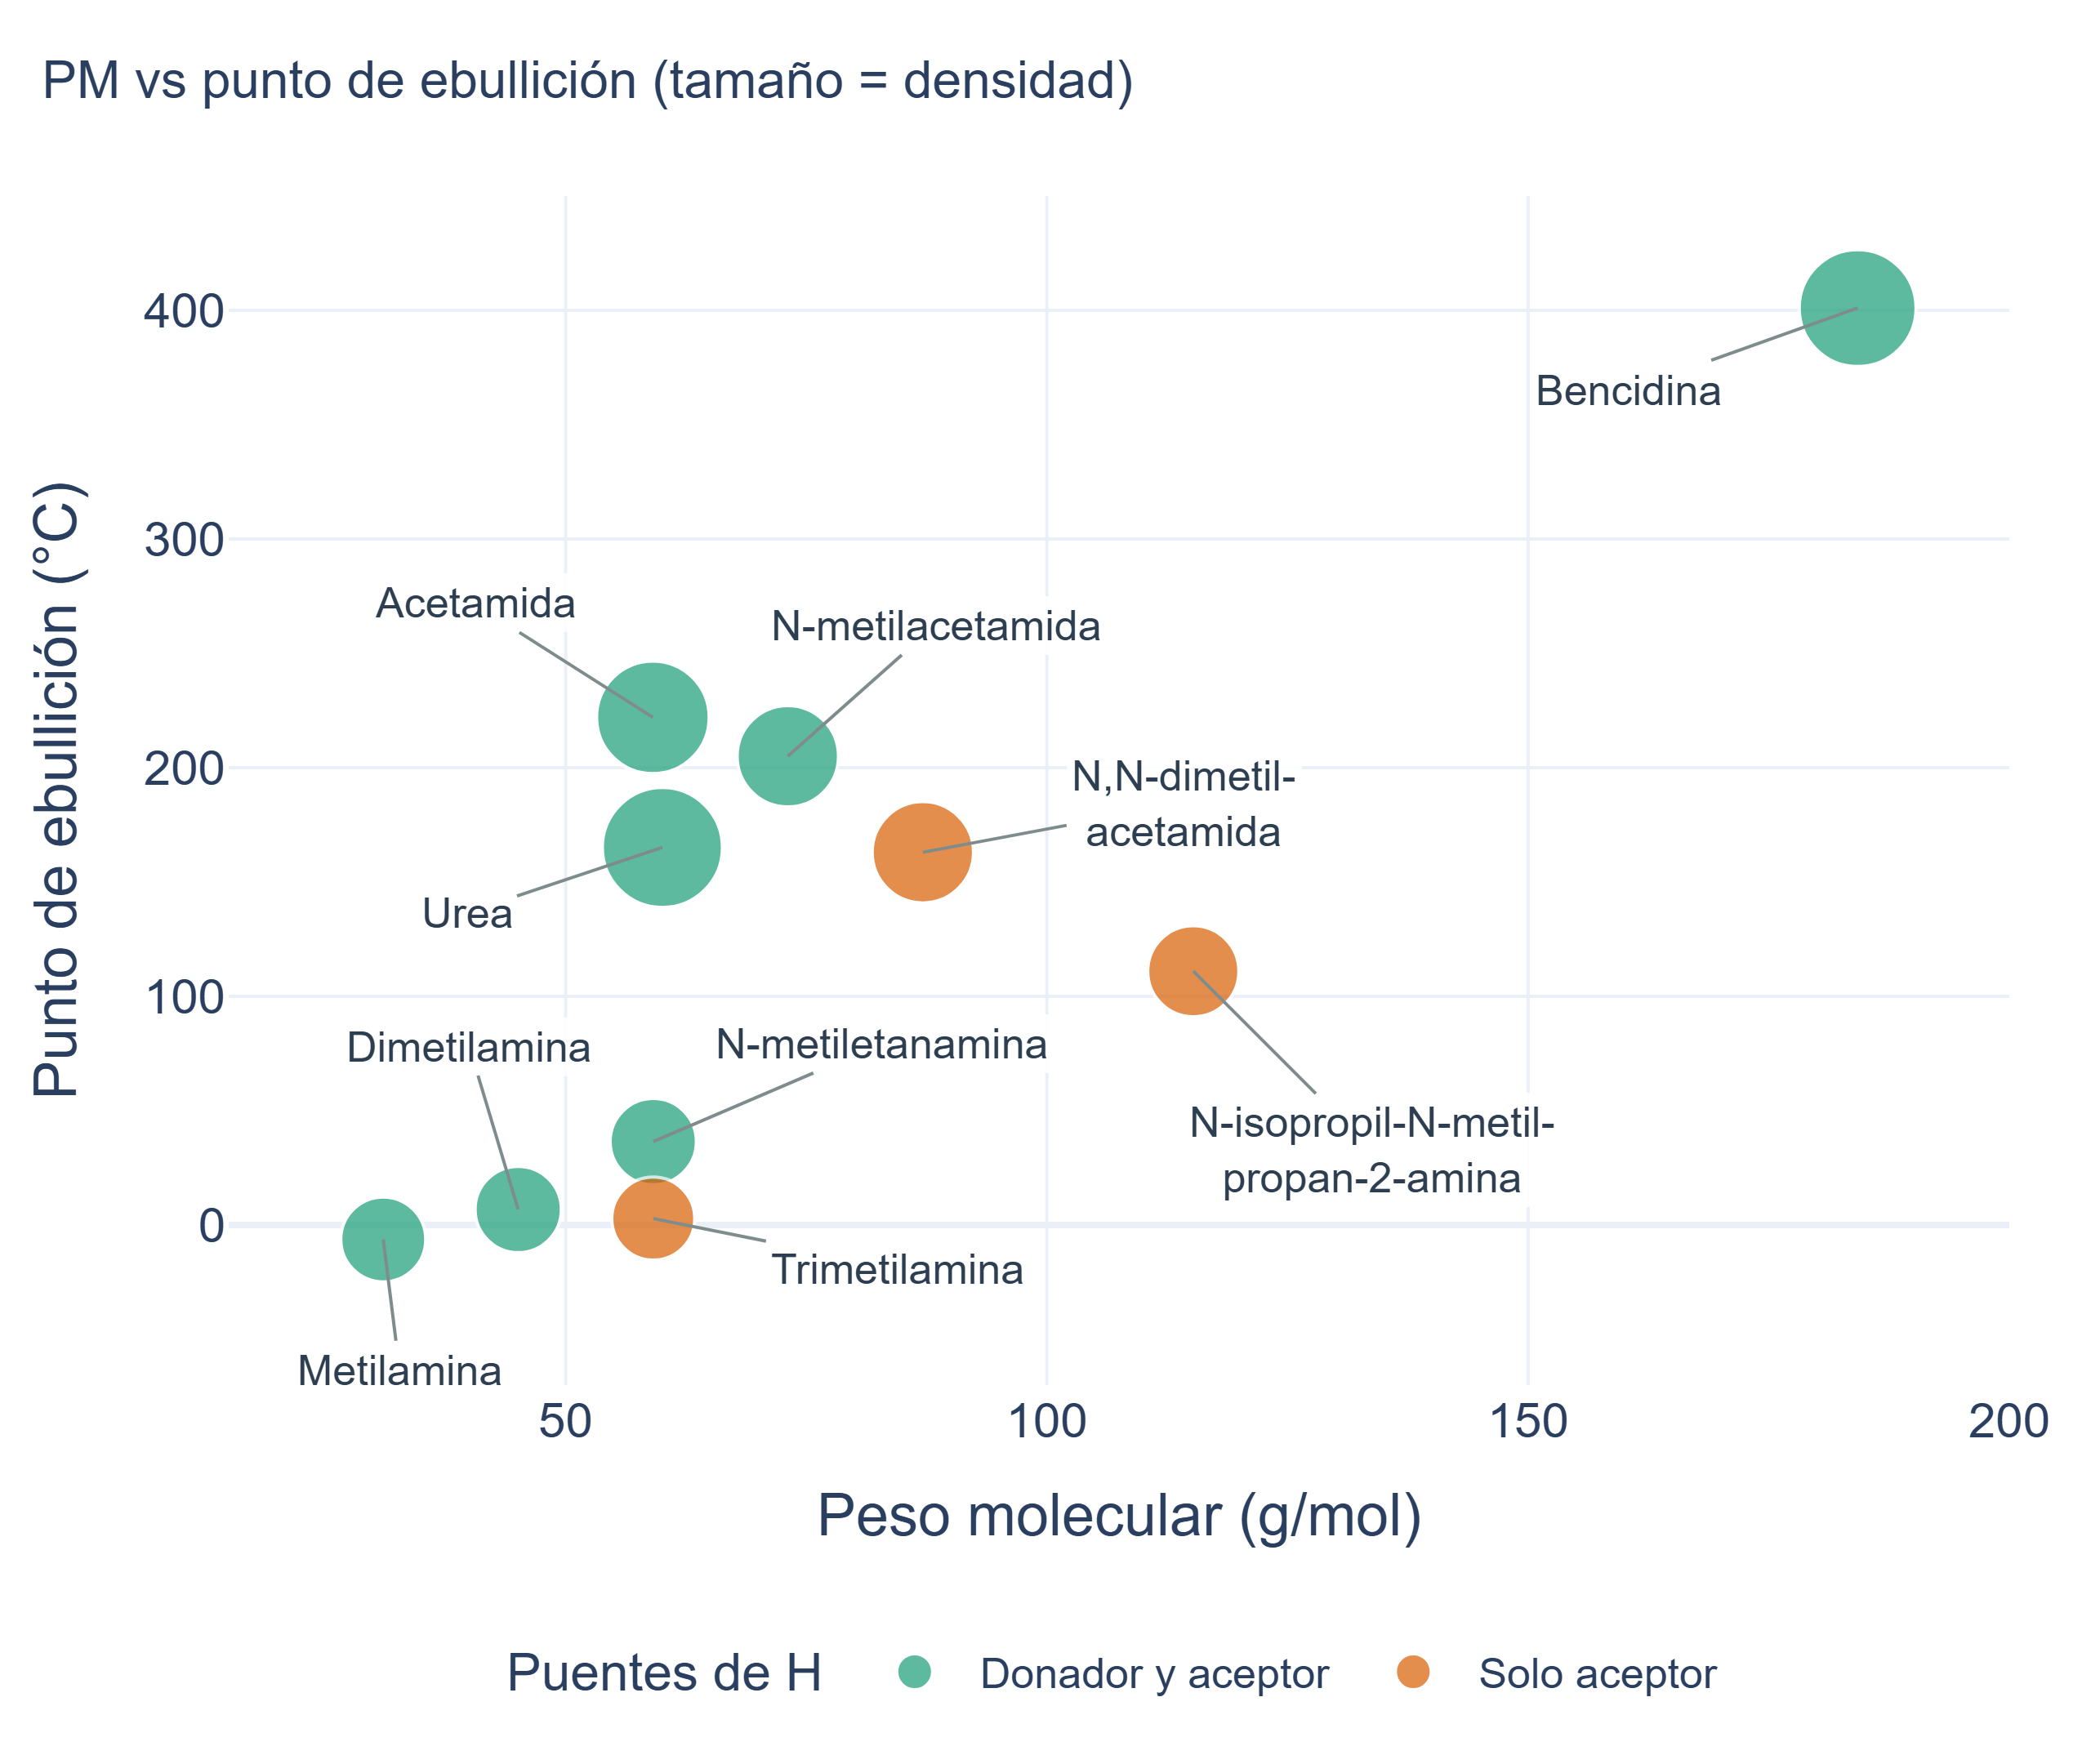
\includegraphics[width=\columnwidth]{11_plotly_burbujas_pm_peb.png}
	\caption{Peso molecular frente a punto de ebullición; el tamaño representa la densidad y el color la capacidad de formar puentes de hidrógeno.}
	\label{fig:burbujas}
\end{figure}

\begin{figure}[htbp]
	\centering
	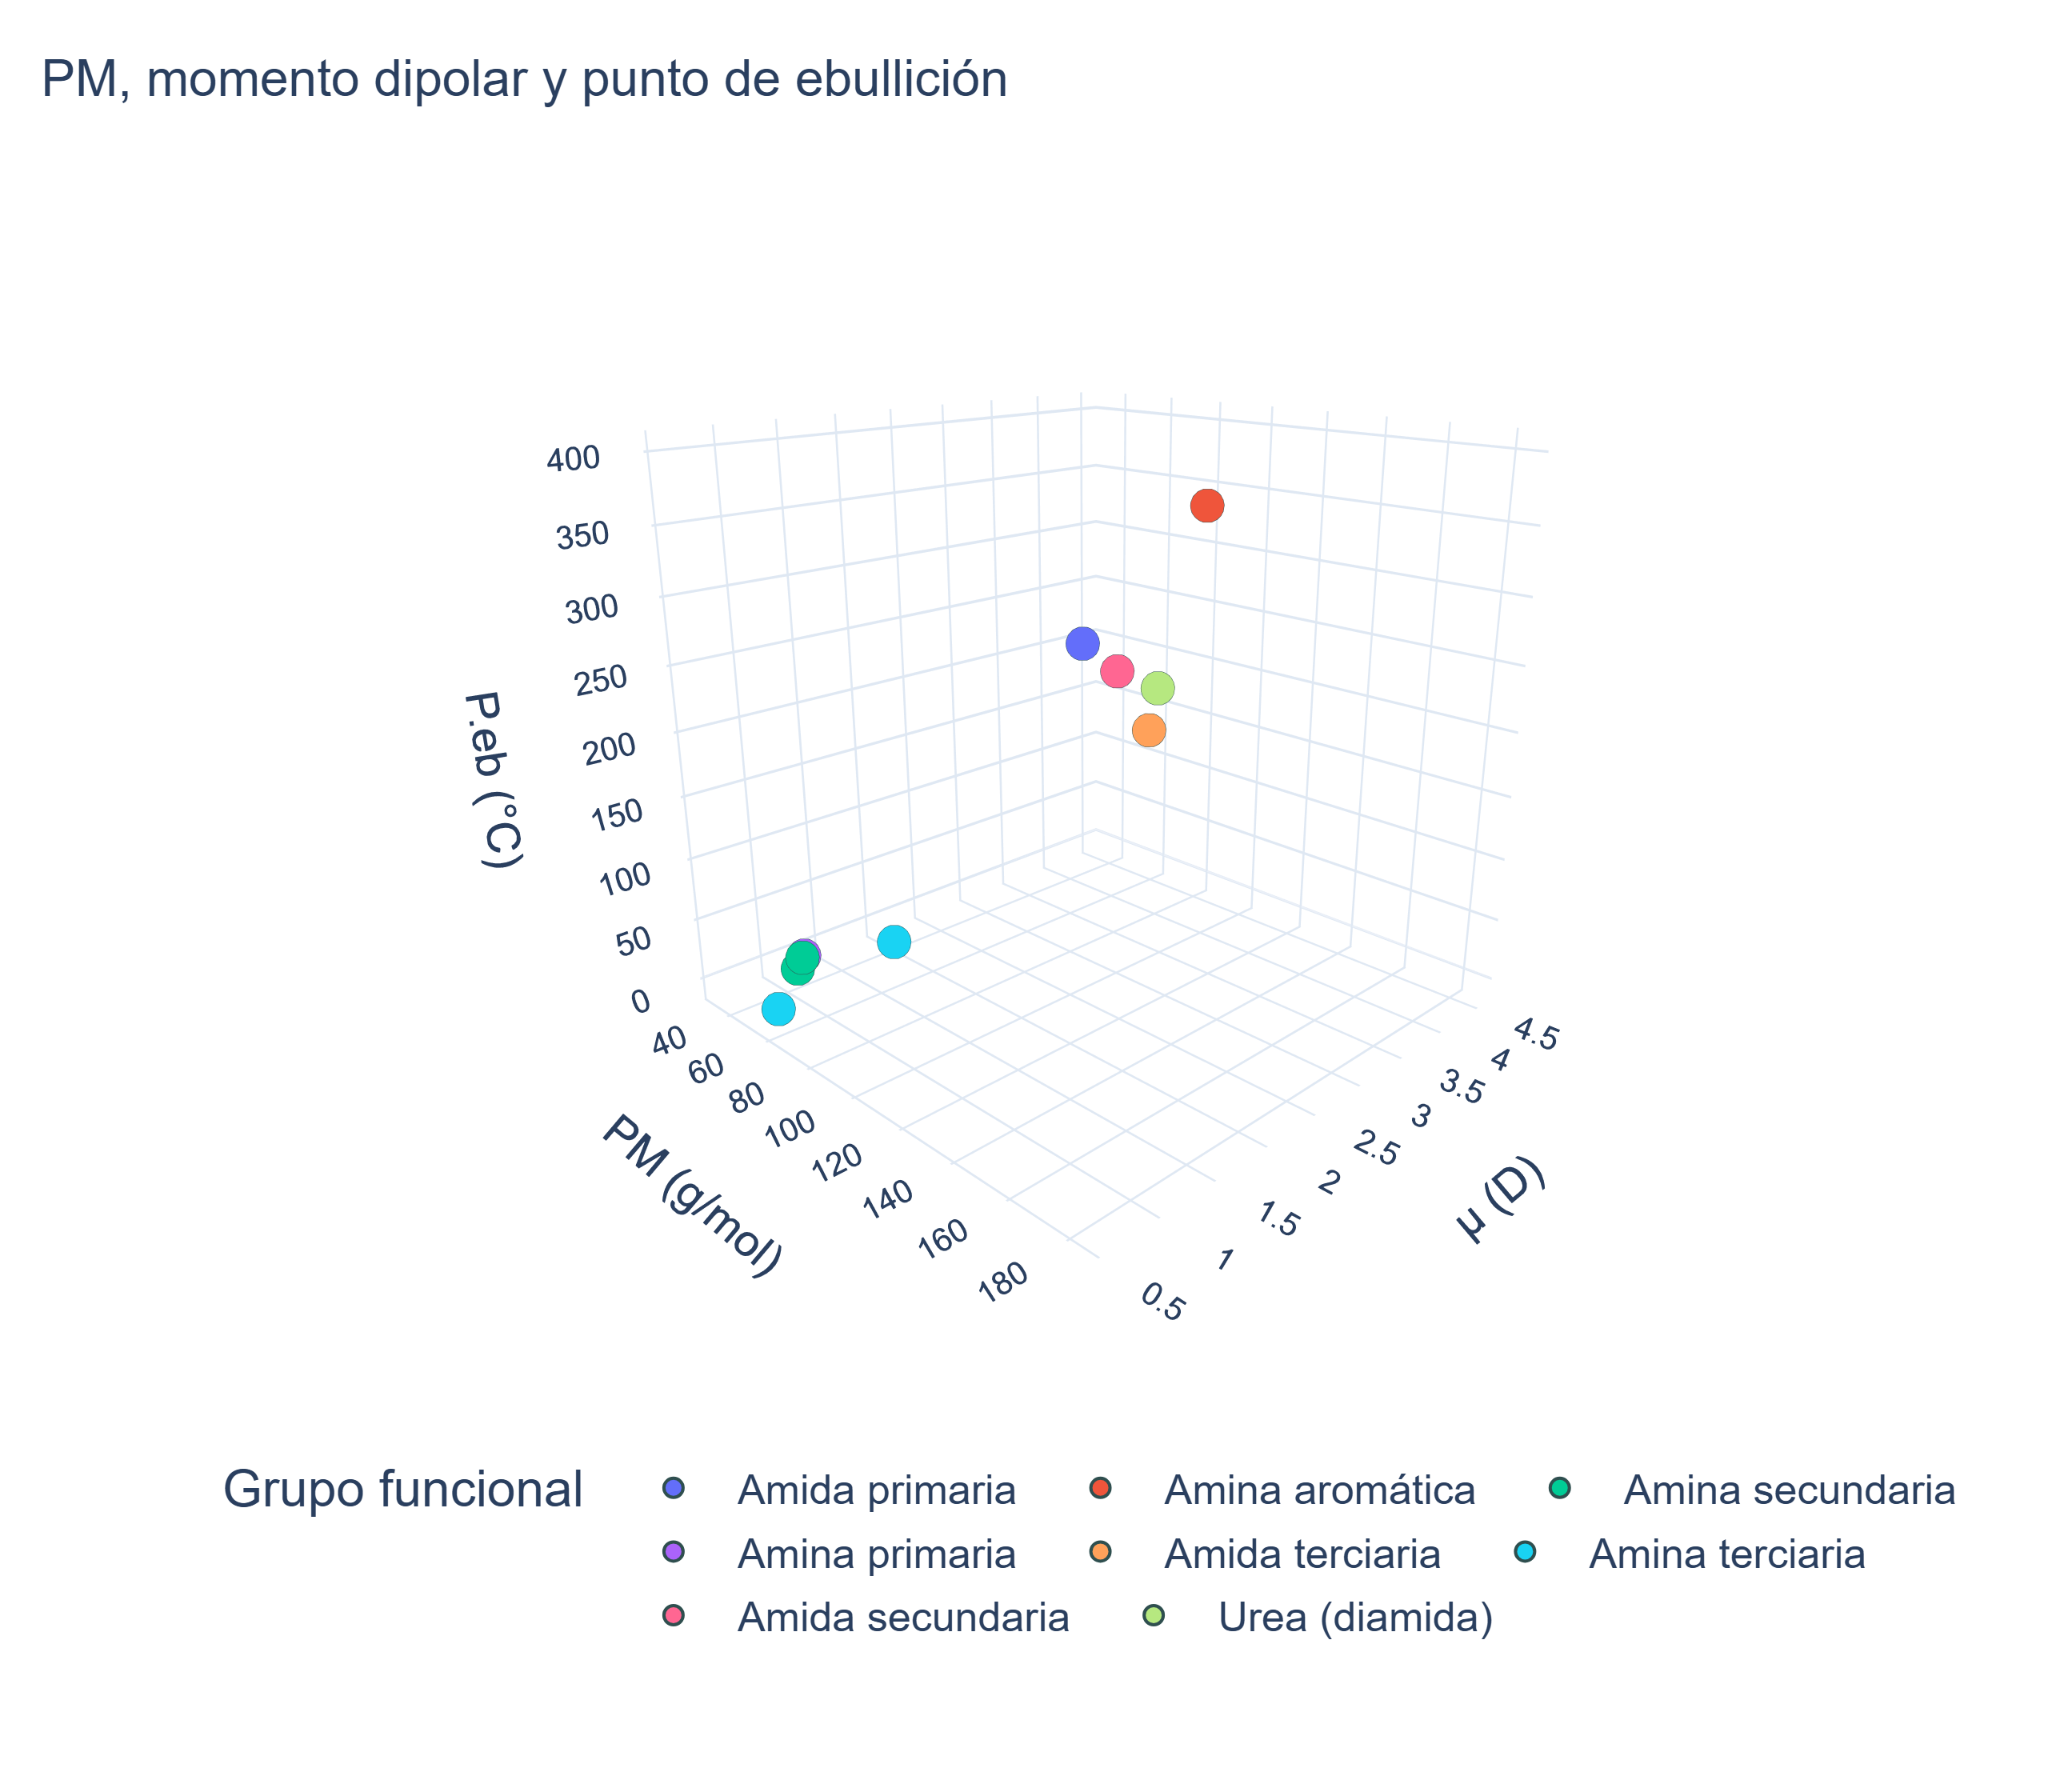
\includegraphics[width=\columnwidth]{12_plotly_3d_pm_dipolo_peb.png}
	\caption{Espacio tridimensional de peso molecular, momento dipolar y punto de ebullición por grupo funcional.}
	\label{fig:3d}
\end{figure}

\begin{figure}[htbp]
	\centering
	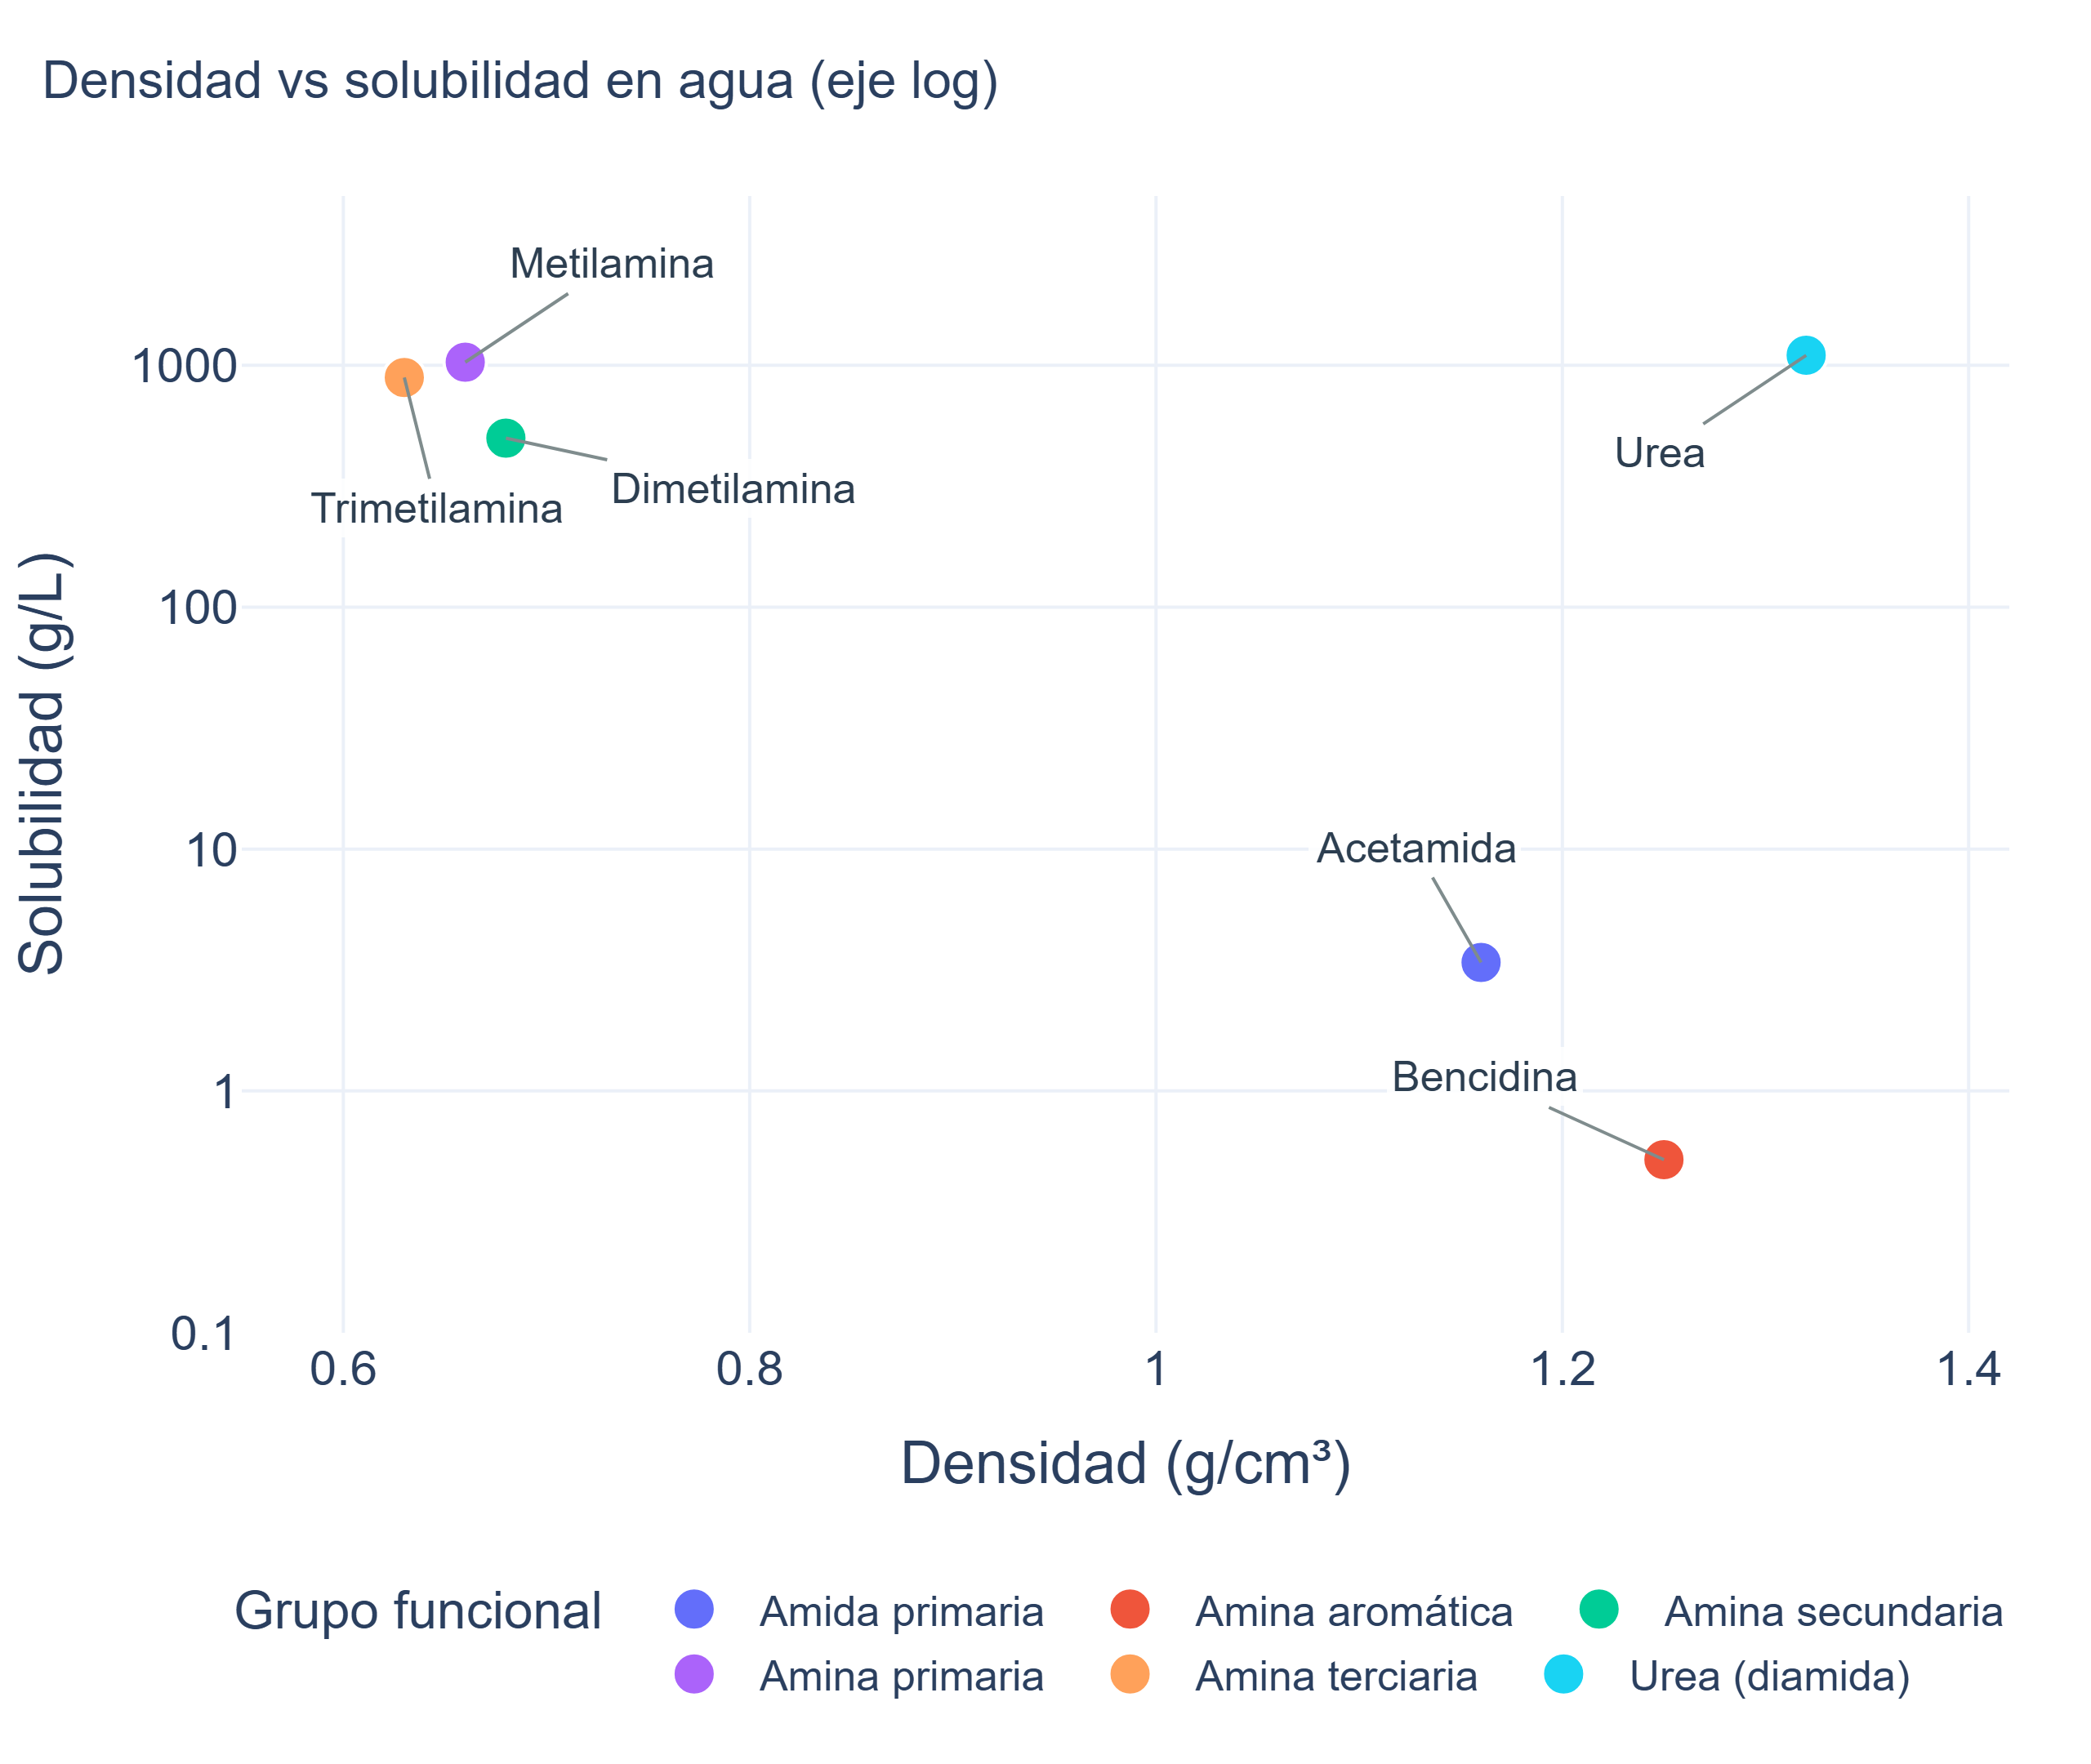
\includegraphics[width=\columnwidth]{13_plotly_densidad_solubilidad.png}
	\caption{Densidad frente a solubilidad en agua (eje logarítmico).}
	\label{fig:dens-sol}
\end{figure}

\subsection{Distribución por tipo de reacción y medio}
% TODO (Valentina): explicar qué representa TR y comparar medianas/dispersiones.
La Figura~\ref{fig:frecuencias} compara la frecuencia de cada mecanismo de
reacción y de cada medio; la sustitución nucleofílica (SN) domina, coherente con
el carácter nucleófilo del par libre del nitrógeno. Las
Figuras~\ref{fig:violin}--\ref{fig:dona} describen la distribución de
probabilidad de TR según el tipo de reacción y el medio.
\textit{[Interpretación pendiente.]}

\begin{figure}[htbp]
	\centering
	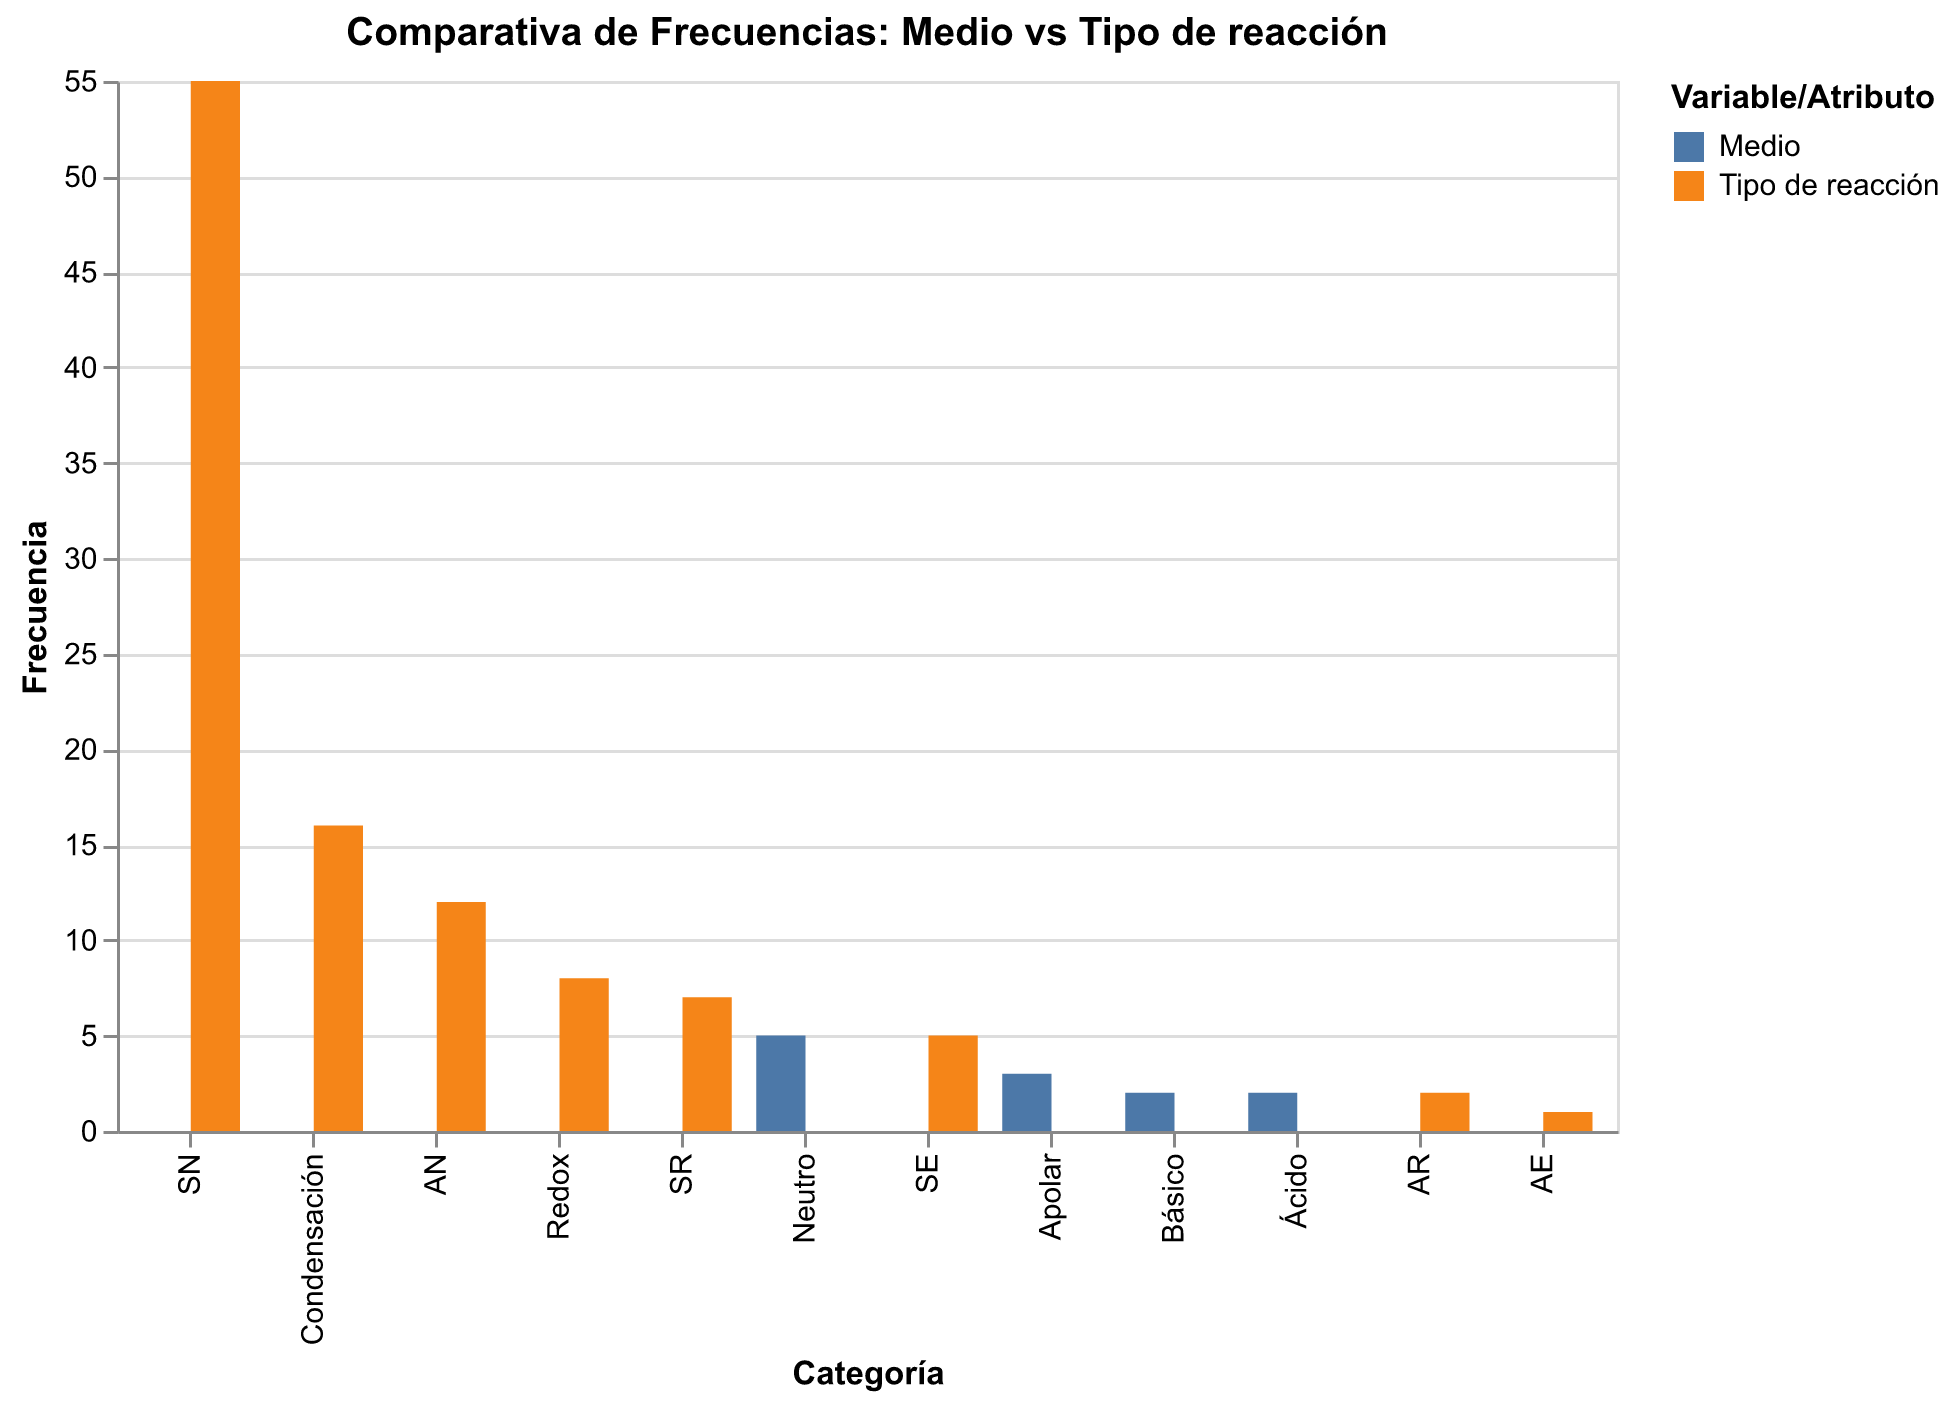
\includegraphics[width=\columnwidth]{09_frecuencias_medio_tipo.png}
	\caption{Frecuencia de los tipos de reacción y de los medios reportados.}
	\label{fig:frecuencias}
\end{figure}

\begin{figure}[htbp]
	\centering
	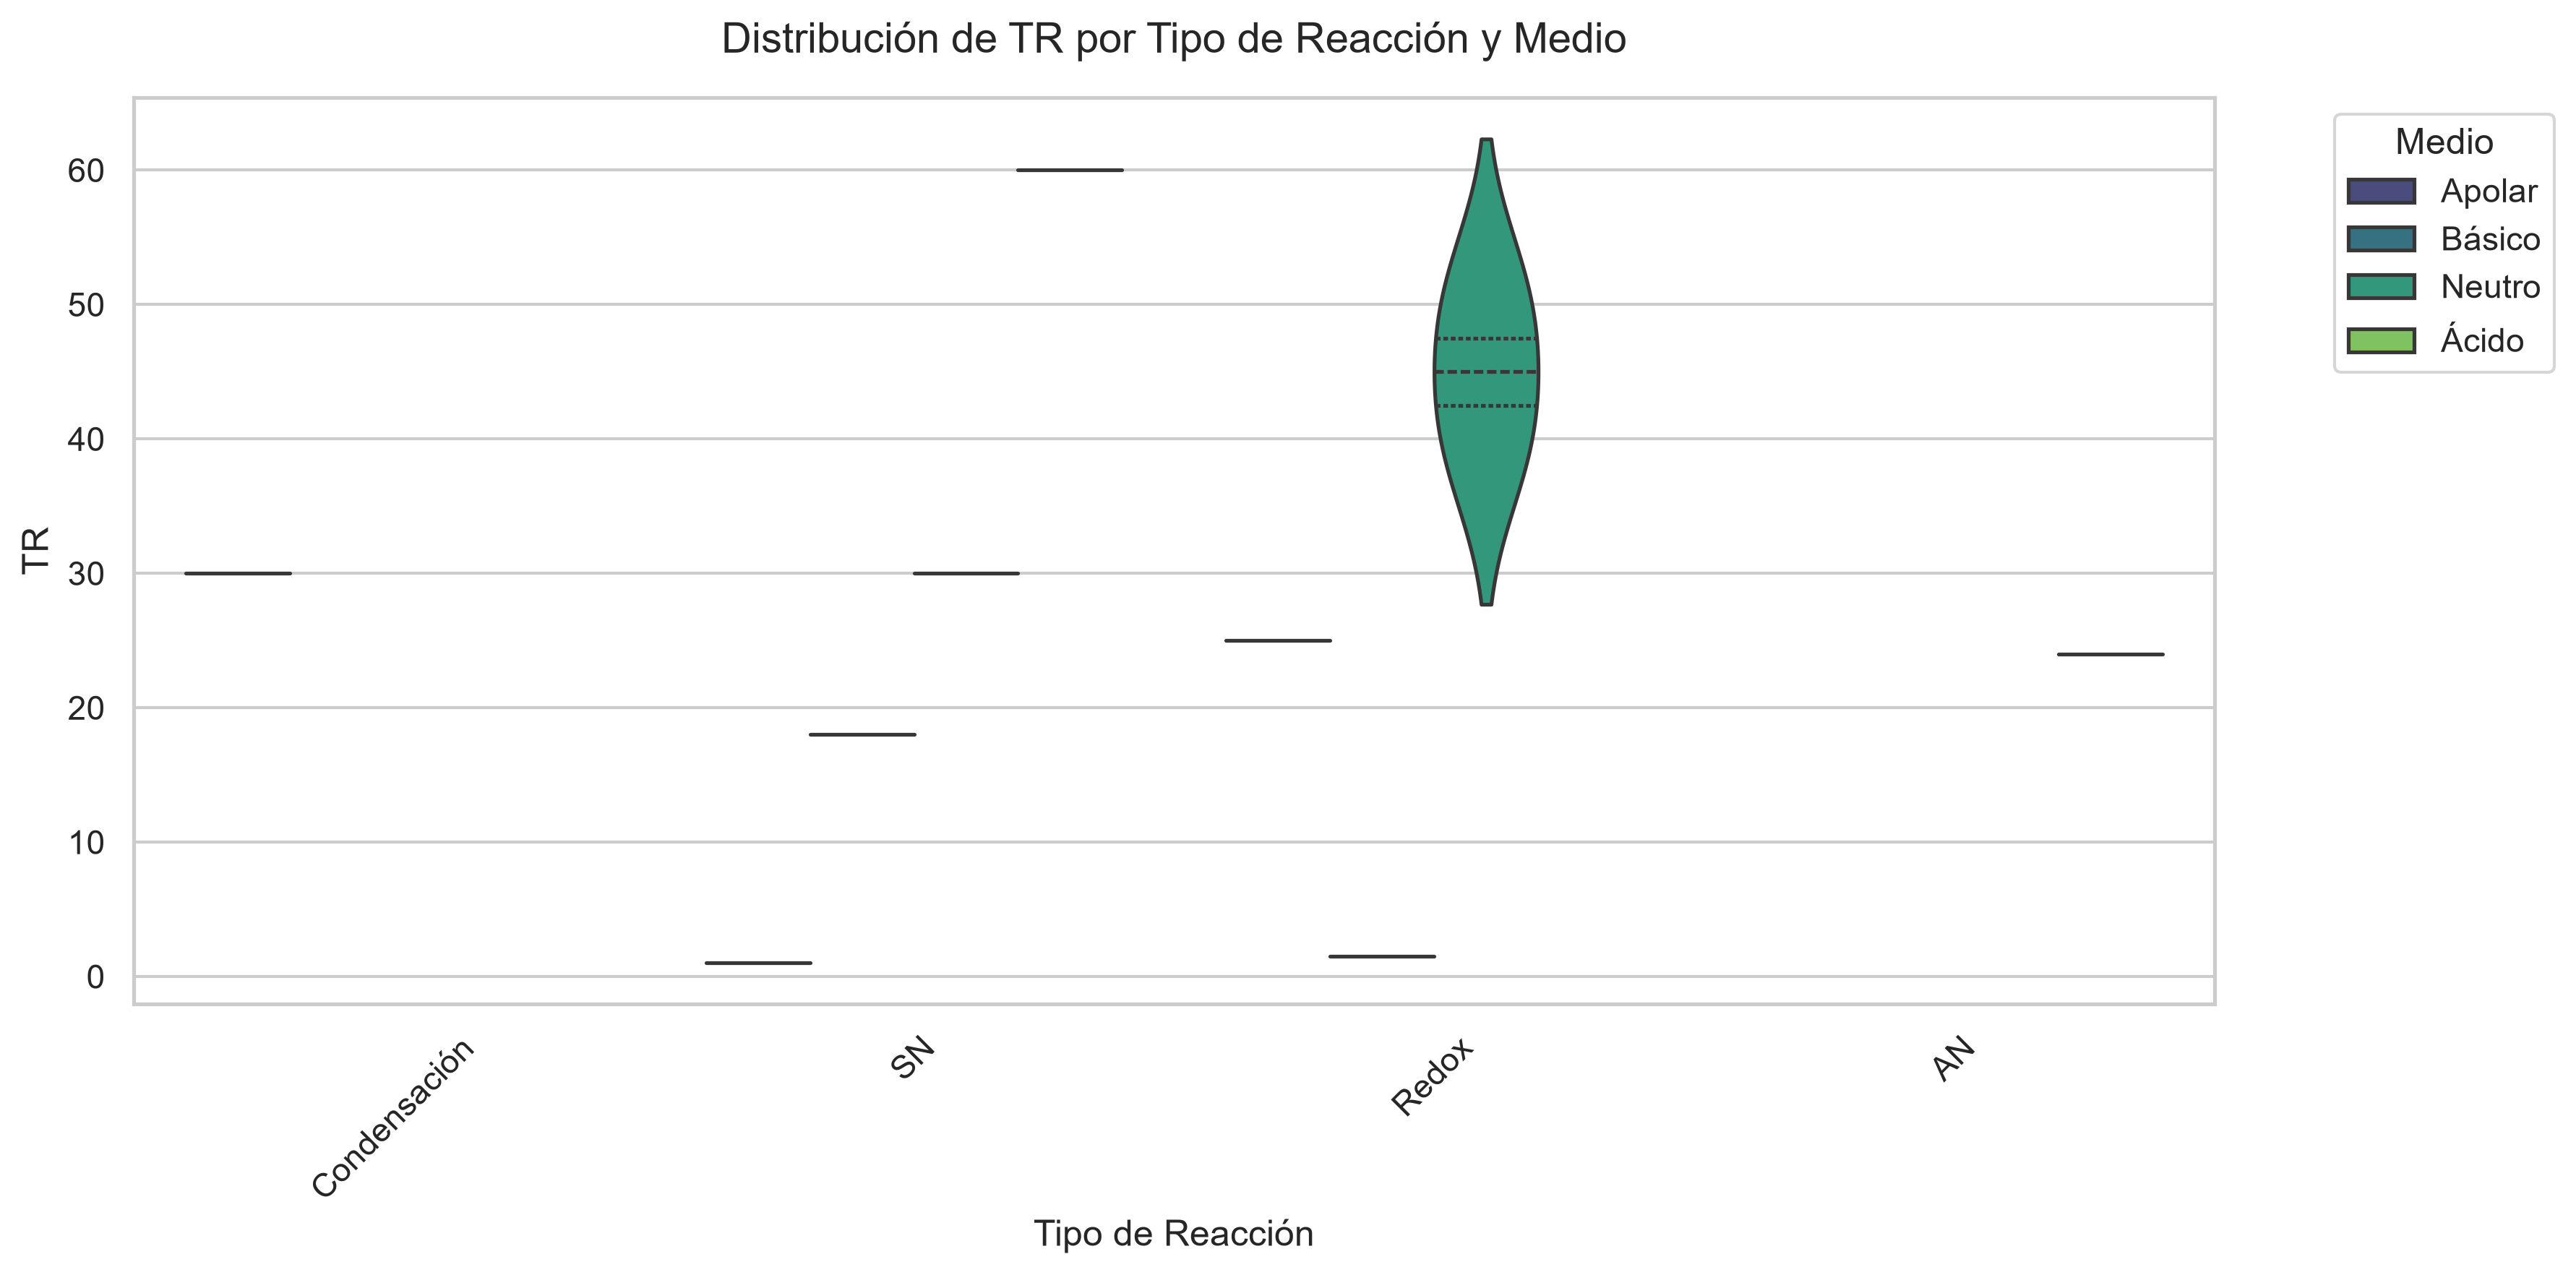
\includegraphics[width=\columnwidth]{07_violin_TR_tipo_medio.png}
	\caption{Distribución (violín) de TR por tipo de reacción y medio.}
	\label{fig:violin}
\end{figure}

\begin{figure}[htbp]
	\centering
	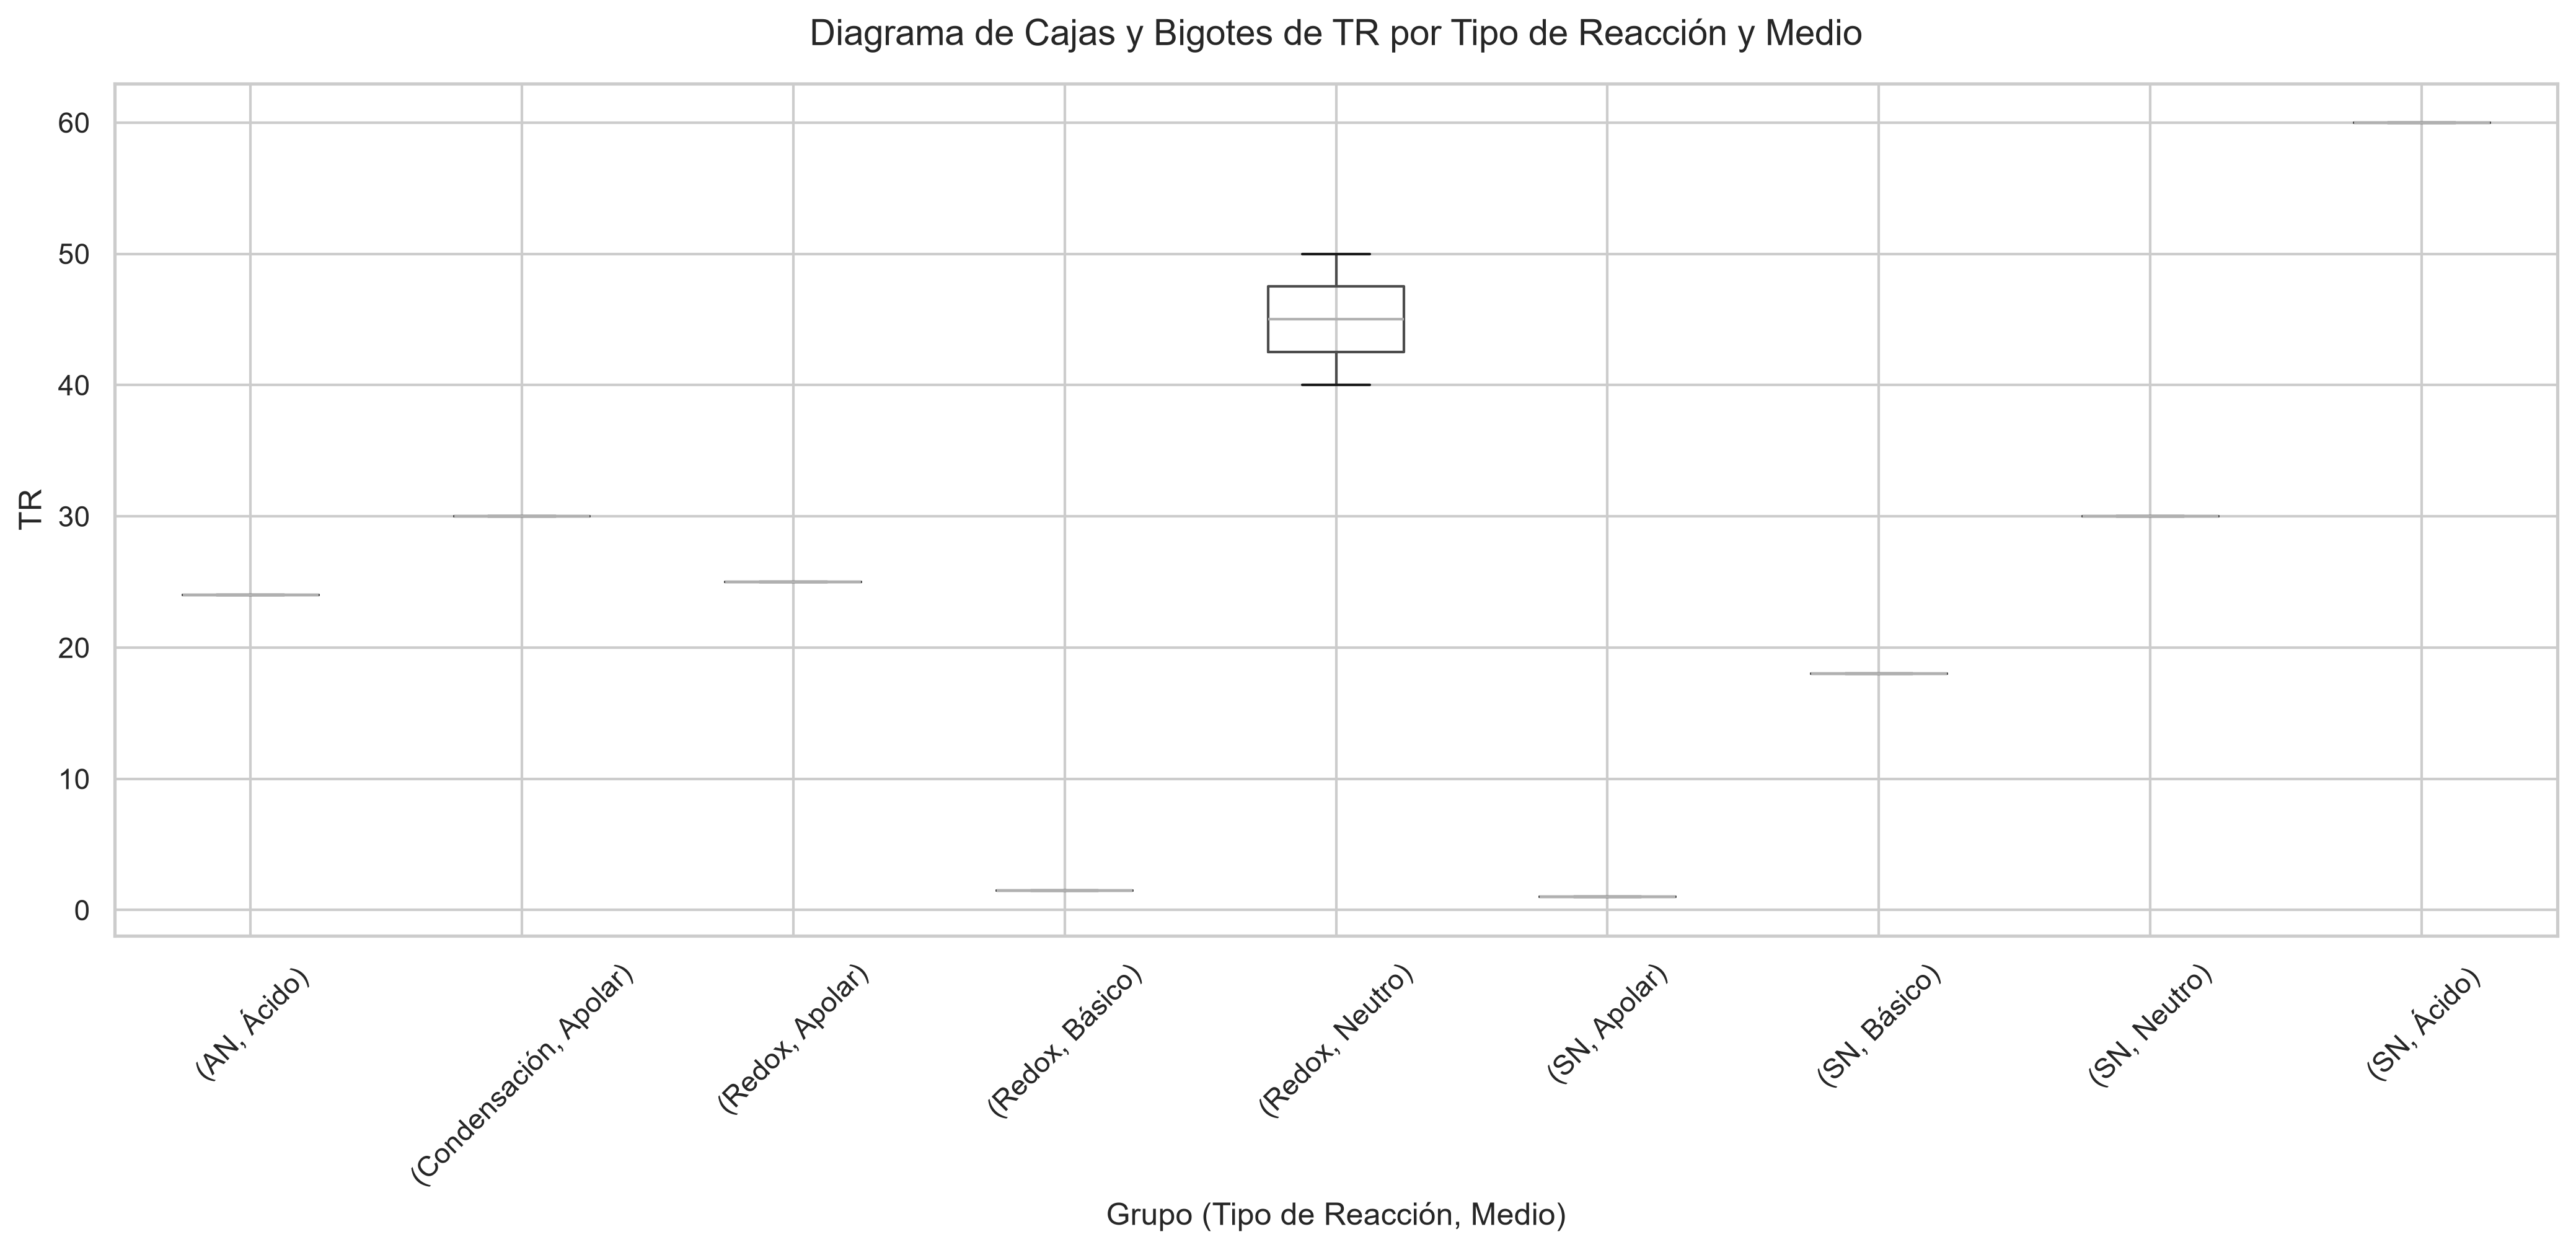
\includegraphics[width=\columnwidth]{08_boxplot_TR_tipo_medio.png}
	\caption{Diagrama de cajas y bigotes de TR por tipo de reacción y medio.}
	\label{fig:boxplot}
\end{figure}

\begin{figure}[htbp]
	\centering
	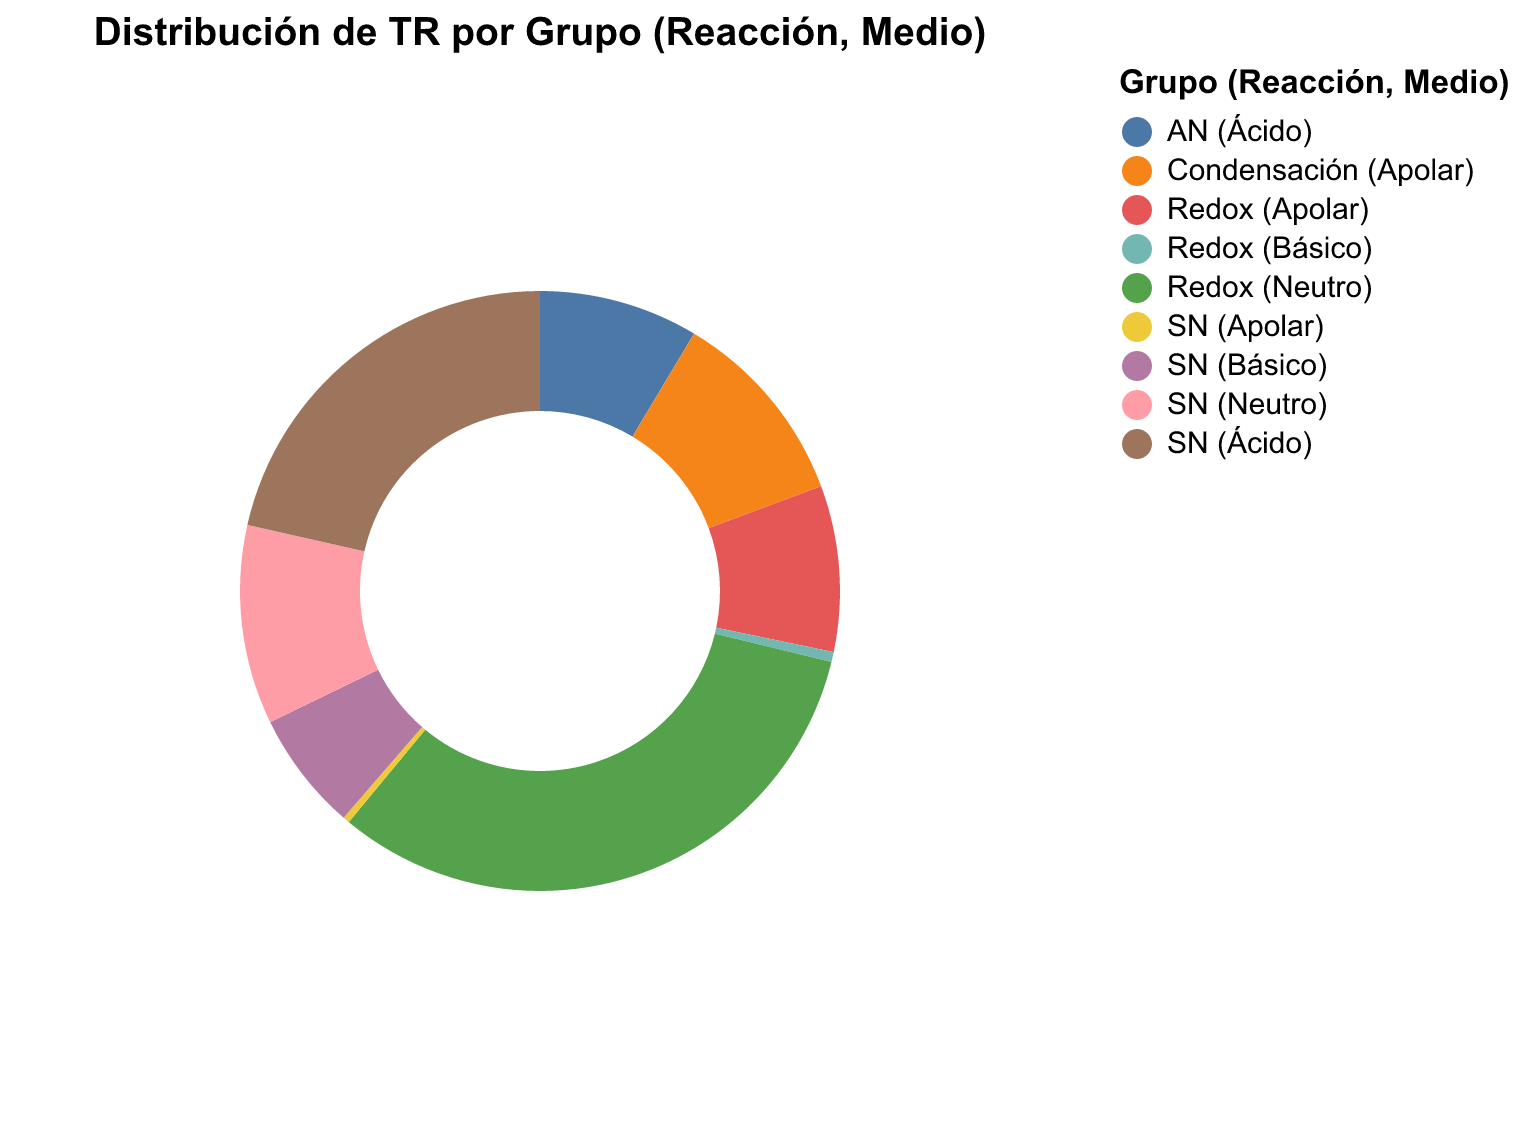
\includegraphics[width=0.9\columnwidth]{10_dona_TR_grupo.png}
	\caption{Participación de TR por grupo (tipo de reacción, medio).}
	\label{fig:dona}
\end{figure}

\section{Conclusiones y Perspectiva}
\fontsize{12}{14}\selectfont
% TODO (Valentina): 3--5 conclusiones que respondan al objetivo de la introducción,
% cada una sustentada en una figura o en la Tabla~\ref{tab:propiedades}.
\textit{[Redacción pendiente.]}
